\documentclass[10pt, final, openany, twoside]{memoir}

%\usepackage[utf8x]{inputenc}
\usepackage{discretebook-small}
\makeindex

\pagestyle{mypagestyle}
\chapterstyle{mychapstyle}

%\showinstnotes
\hideinstnotes

\finishhwsol %initially, any solution environment is not a homework solution.

% % % % Set up file for answers to practice problems: % % % % %
\def\ansfilename{practice-answers}
\Opensolutionfile{\ansfilename}
\Newassociation{answer}{ans}{\ansfilename}

%glossaries:
\glsdisablehyper
\loadglsentries{symbols}
\makenoidxglossaries


% % % % % % % % % % % % % % % % % % % % % % % % % % % % % % % % % % % % %
% % % % % % % % 					% % % % % % % % % % % % % % % % % % %
% % % % % % % % Begin main document % % % % % % % % % % % % % % % % % % %
% % % % % % % %                     % % % % % % % % % % % % % % % % % % %
% % % % % % % % % % % % % % % % % % % % % % % % % % % % % % % % % % % % %


\begin{document}



\frontmatter
\input{frontmatter/cover}

\clearpage

\input{frontmatter/title-page}

{\small \input{frontmatter/copyright-page}}

\tableofcontents

\input{frontmatter/preface}



\mainmatter

\setcounter{chapter}{-1}
\chapter[Introduction]{Introduction and Preliminaries}

	\input{chapters/Introduction}

	\section{Sets}\label{sec:sets}
	\input{chapters/Sets}
	\withanswers\input{exercises/Sets}

	\section{Functions}\label{sec:functions}
	\input{chapters/Functions}
	\withanswers\input{exercises/Functions}

\chapter[Counting]{Counting}\label{ch:counting}

	\input{chapters/Counting-Intro}

	\documentclass[12pt]{article}

\usepackage{discrete}

\def\thetitle{Introduction to Counting} % will be put in the center header on the first page only.
\def\lefthead{Math 228 Notes} % will be put in the left header
\def\righthead{Counting} % will be put in the right header


\begin{document}

\section{Additive and Multiplicative Principles}\label{sec:additiveMultiplicative}

\begin{activity}
\begin{questions}
\question A restaurant offers 8 appetizers and 14 entr\'ees.  How many choices do you have if:
\begin{parts}
 \part you will eat one dish, either an appetizer or an entr\'ee?
 \part you are extra hungry and want to eat both an appetizer and an entr\'ee?
\end{parts}
\question Think about the methods you used to solve question 1.  Write down the rules for these methods.
\question Do your rules work?  A standard deck of playing cards has 26 red cards and 12 face cards.

\begin{parts}
 \part How many ways can you select a card which is either red or a face card?
 \part How many ways can you select a card which is both red and a face card?
 \part How many ways can you select two cards so that the first one is red and the second one is a face card?
\end{parts}
\end{questions}

\end{activity}


Consider this rather simple counting problem: at Red Dogs and Donuts, there are 14 varieties of donuts, and 16 types of hot dogs.  If you want either a donut or a dog, how many options do you have?  This isn't too hard, you just add 14 and 16.  Will that always work?  What is important here?


\begin{defbox}{Additive Principle}
  The {\em additive principle}\index{additive principle} states that if event $A$ can occur in $m$ ways, and event $B$ can occur in $n$ {\em disjoint}\index{disjoint} ways, then the event ``$A$ or $B$'' can occur in $m + n$ ways.
\end{defbox}

It is important that the events be disjoint.  For example, a standard deck of 52 cards contains $26$ red cards and $12$ face cards.  However, the number of ways to select a card which is either red or a face card is not $26 + 12 = 38$.  This is because there are 6 cards which are both red and face cards.

The additive principle works with more than two events.  Say, in addition to your 14 choices for donuts and 16 for dogs, you would also consider eating one of 15 waffles?  How many choices do you have now?  You would have $14 + 16 + 15 = 45$ options.

\begin{example}
  How many two letter ``words''\index{words} start with either A or B?  How many start with one of the 5 vowels?  (A word is just a strings of letters; it doesn't have to be English, or even pronounceable.)

  \begin{solution}
    First, how many two letter words start with A?  We just need to select the second letter, which can be accomplished in 26 ways.  So there are 26 words starting with A.  There are also 26 words that start with B.  To select a word which starts with either A or B, we can pick the word from the first 26 or the second 26, for a total of 52 words.  The additive principle is at work here.

    Now what about all the two letter words starting with a vowel?  There are 26 starting with A, another 26 starting with E, and so on.  We will have 5 groups of 26.  So we add 26 to itself 5 times.  Of course it would be easier to just multiply $5\cdot 26$.  We are really using the additive principle again, just using multiplication as a shortcut.
  \end{solution}

\end{example}

\begin{example}
  Suppose you are going for some fro-yo.  You can pick one of 6 yogurt choices, and one of 4 toppings.  How many choices do you have?

  \begin{solution}
    Break your choices up into disjoint events:  $A$ are the choices with the first topping, $B$ the choices featuring the second topping, and so on.  There are four events; each can occur in 6 ways (one for each yogurt flavor).  The events are disjoint, so the total number of choices is $6 + 6 + 6 + 6 = 24$.
  \end{solution}


\end{example}

Note that in both of the previous examples, when using the additive principle on a bunch of events all the same size, it is quicker to multiply.  This really is the same, and not just because $6 + 6 + 6 + 6 = 4\cdot 6$.  We can first select the topping in 4 ways (that is, we first select which of the disjoint events we will take).  For each of those first 4 choices, we now have 6 choices of yogurt.  We have:

\begin{defbox}{Multiplicative Principle}
  The {\em multiplicative principle}\index{multiplicative principle} states that if event $A$ can occur in $m$ ways, and each possibility for $A$ allows for exactly $n$ ways for event $B$, then the event ``$A$ and $B$'' can occur in $m \cdot n$ ways.
\end{defbox}

The multiplicative principle generalizes to more than two events as well.

\begin{example}
  How many license plates can you make out of three letters followed by three numerical digits?

  \begin{solution}
    Here we have six events: the first letter, the second letter, the third letter, the first digit, the second digit, and the third digit.  The first three events can each happen in 26 ways; the last three can each happen in 10 ways.  So the total number of license plates will be $26\cdot 26\cdot 26 \cdot 10 \cdot 10 \cdot 10$, using the multiplicative principle.

    Does this make sense?  Think about how we would pick a license plate. How many choices we would have?  First, we need to pick the first letter.  There are 26 choices.  Now for each of those, there are 26 choices for the second letter: 26 second letters with first letter A, 26 second letters with first letter B, and so on.  We add 26 to itself 26 times.  Or quicker: there are $26 \cdot 26$ choices for the first two letters.

    Now for each choice of the first two letters, we have 26 choices for the third letter.  That is, 26 third letters for the first two letters AA, 26 choices for the third letter after starting AB, and so on.  There are $26 \cdot 26$ of these $26$ third letter choices, for a total of $(26\cdot26)\cdot 26$ choices for the first three letters.  And for each of these $26\cdot26\cdot26$ choices of letters, we have a bunch of choices for the remaining digits.

    In fact, there are going to be exactly 1000 choices for the numbers.  We can see this because there are 1000 three-digit numbers (000 through 999).  This is 10 choices for the first digit, 10 for the second, and 10 for the third.  The multiplicative principle says we multiply: $10\cdot 10 \cdot 10 = 1000$.

    All together, there were $26^3$ choices for the three letters, and $10^3$ choices for the numbers, so we have a total of $26^3 \cdot 10^3$ choices of license plates.
  \end{solution}

\end{example}


 Careful: ``and'' doesn't mean ``times.''  For example, how many playing cards are both red and a face card?  Not $26 \cdot 12$.  The answer is 6, and we needed to know something about cards to answer that question.

 Another caution: how many ways can you select two cards, so that the first one is a red card and the second one is a face card?  This looks more like the multiplicative principle (you are counting two separate events) but the answer is not $26 \cdot 12$ here either.  The problem is that while there are 26 ways for the first card to be selected, it is not the case that {\em for each} of those there are 12 ways to select the second card.  If the first card was both red and a face card, then there would be only 11 choices for the second card.  The moral of this story is that the multiplicative principle only works if the events are independent.\footnote{To solve this problem, you could break it into two cases. First, count how many ways there are to select the two cards when the first card is a red non-face card. Second, count how many ways when the first card is a red face card.  Doing so makes the events in each separate case independent, so the multiplicative principle can be applied.}

\subsection{Counting With Sets}\label{subsec:countingWithSets}


Do you believe the additive and multiplicative principles?  How would you convince someone they are correct?  This is surprisingly difficult.  They seem so simple, so obvious.  But why do they work?

To make things clearer, and more mathematically rigorous, we will use sets.  Do not skip this section!  It might seem like we are just trying to give a proof of these principles, but we are doing a lot more.  If we understand the additive and multiplicative principles rigorously, we will be better at applying them, and knowing when and when not to apply them at all.

We will look at the additive and multiplicative principles in a slightly different way.  Instead of thinking about event $A$ and event $B$, we want to think of a set $A$ and a set $B$.  The sets will contain all the different ways the event can happen.  (It will be helpful to be able to switch back and forth between these two models when checking that we have counted correctly.)  Here's what we mean:

\begin{example}
 Suppose you own 9 shirts and 5 pairs of pants.
 \begin{enumerate}
  \item How many outfits can you make?
  \item If today is half-naked-day, and you will wear only a shirt or only a pair of pants, how many choices do you have?
 \end{enumerate}
\begin{solution}
 By now you should agree that the answer to the first question is $9 \cdot 5 = 45$ and the answer to the second question is $9 + 5 = 14$.  These are the multiplicative and additive principles.  There are two events: picking a shirt and picking a pair of pants.  The first event can happen in 9 ways and the second event can happen in 5 ways.  To get both a shirt and a pair of pants, you multiply.  To get just one article of clothing, you add.

 Now look at this using sets.  There are two sets, call them $S$ and $P$.  The set $S$ contains all 9 shirts so $|S| = 9$ while $|P| = 5$, since there are 5 elements in the set $P$ (namely your 5 pairs of pants).  What are we asking in terms of these sets?  Well in question 2, we really want $|S \cup P|$, the number of elements in the union of shirts and pants.  This is just $|S| + |P|$ (since there is no overlap; $|S \cap P| = 0$).  Question 1 is slightly more complicated.  Your first guess might be to find $|S \cap P|$, but this is not right (there is nothing in the intersection).  We are not asking for how many clothing items are both a shirt and a pair of pants.  Instead, we want one of each.  We could think of this as asking how many pairs $(x,y)$ there are, where $x$ is a shirt and $y$ is a pair of pants.  As we will soon verify, this number is $|S| \cdot |P|$.
\end{solution}
\end{example}

From this example we can see right away how to rephrase our additive principle in terms of sets:

\begin{defbox}{Additive Principle (with sets)\index{additive principle}}
Given two sets $A$ and $B$, if $A \cap B = \emptyset$ (that is, if there is no element in common to both $A$ and $B$), then
\[|A \cup B| = |A| + |B|.\]
\end{defbox}

This hardly needs a proof.  To find $A \cup B$, you take everything in $A$ and throw in everything in $B$.  Since there is no element in both sets already, you will have $|A|$ things and add $|B|$ new things to it.  This is what adding does!  Of course, we can easily extend this to any number of disjoint sets.

From the example above, we see that in order to investigate the multiplicative principle carefully, we need to consider ordered pairs.  We should define this carefully:

\begin{defbox}{Cartesian Product}
 Given sets $A$ and $B$, we can form the \emph{set} $A \times B = \{(x,y) \st x \in A \wedge y \in B\}$ to be the set of all ordered pairs $(x,y)$ where $x$ is an element of $A$ and $y$ is an element of $B$.  We call $A \times B$ the \emph{Cartesian product}\index{Cartesian product} of $A$ and $B$.
\end{defbox}

The question is, what is $|A \times B|$?  To figure this out, write out $A \times B$.

Let $A = \{a_1,a_2, a_3, \ldots, a_m\}$ and $B = \{b_1,b_2, b_3, \ldots, b_n\}$  (so $|A| = m$ and $|B| = n$).  The set $A \times B$ contains all pairs with the first half of the pair being $a_i$ for some $i$ and the second being $b_j$ for some $j$.  In other words:
\begin{align*}
 A \times B = \{ & (a_1, b_1), (a_1, b_2), (a_1, b_3), \ldots (a_1, b_n), \\
  & (a_2, b_1), (a_2, b_2), (a_2, b_3), \ldots, (a_2, b_n), \\
  & (a_3, b_1), (a_3, b_2), (a_3, b_3), \ldots, (a_3, b_n), \\
  & \vdots \\
  & (a_m, b_1), (a_m, b_2), (a_m, b_3), \ldots, (a_m, b_n)\}.
\end{align*}

Notice what we have done here: we made $m$ rows of $n$ pairs, for a total of $m \cdot n$ pairs.

Each row above is really $\{a_i\} \times B$ for some $a_i \in A$.  That is, we fixed the $A$-element.  Broken up this way, we have
\[A \times B = (\{a_1\} \times B) \cup (\{a_2\} \times B) \cup (\{a_3\}\times B) \cup \cdots \cup (\{a_m\} \times B).\]
So $A \times B$ is really the union of $m$ disjoint sets.  Each of those sets has $n$ elements in them.  The total (using the additive principle) is $n + n + n + \cdots + n = m \cdot n$.

To summarize:

\begin{defbox}{Multiplicative Principle (with sets)\index{multiplicative principle}}
 Given two sets $A$ and $B$, we have $|A \times B| = |A| \cdot |B|$.
\end{defbox}

Again, we can easily extend this to any number of sets.

\subsection{Principle of Inclusion/Exclusion\index{principle of inclusion/exclusion}\index{PIE}}\label{sec:PIE}
%TODO: add investigate activity (perhaps the pie survey?)

While we are thinking about sets, consider what happens to the additive principle when the sets are NOT disjoint. Suppose we want to find $|A \cup B|$ and know that $|A| = 10$ and $|B| = 8$.  This is not enough information though.  We do not know how many of the 8 elements in $B$ are also elements of $A$.  However, if we also know that $|A \cap B| = 6$, then we can say exactly how many elements are in $A$, and, of those, how many are in $B$ and how many are not (6 of the 10 elements are in $B$, so 4 are in $A$ but not in $B$).  We could fill in a Venn diagram \index{Venn diagram} as follows:

\begin{center}

     \begin{tikzpicture}
   \draw[thick] \circleA \circleAlabel \circleB \circleBlabel \twosetbox;
   \draw (0,0) node{6} (-1,0) node{4} (1,0) node{2};
 \end{tikzpicture}


\end{center}

This says there are 6 elements in $A \cap B$, 4 elements in $A \setminus B$ and 2 elements in $B \setminus A$.  Now \emph{these} three sets \emph{are} disjoint, so we can use the additive principle to find the number of elements in $A \cup B$.  It is $6 + 4 + 2 = 12$.

This will always work, but drawing a Venn diagram is more than we need to do.  In fact, it would be nice to relate this problem to the case where $A$ and $B$ are disjoint.  Is there one rule we can make that works in either case?

\todo[inline]{Alees suggests a GCD or LCM question to draw a connection to the other place they have seen this, perhaps as an exercise.  This is a great idea.}

Here is another way to get the answer to the problem above.  Start by just adding $|A| + |B|$.  This is $10 + 8 = 18$, which would be the answer if $|A \cap B| = 0$.  We see that we are off by exactly 6, which just so happens to be $|A \cap B|$.  So perhaps we guess,
\[|A \cup B| = |A| + |B| - |A \cap B|.\]
This works for this one example.  Will it always work?  Think about what we are doing here.  We want to know how many things are either in $A$ or $B$ (or both).  We can throw in everything in $A$, and everything in $B$.  This would give $|A| + |B|$ many elements.  But of course when you actually take the union, you do not repeat elements that are in both.  So far we have counted every element in $A \cap B$ exactly twice: once when we put in the elements from $A$ and once when we included the elements from $B$.  We correct by subtracting out the number of elements we have counted twice.  So we added them in twice, subtracted once, leaving them counted only one time.

In other words, we have:


\begin{defbox}{Cardinality of a union (2 sets)}
  For any finite sets $A$ and $B$,
  \[|A \cup B| = |A| + |B| - |A \cap B|.\]
\end{defbox}


We can do something similar with three sets.

\begin{example}
An examination in three subjects, Algebra, Biology, and Chemistry, was taken
by 41 students. The following table shows how many students failed in each
single subject and in their various combinations:
\vskip 1ex
\begin{center}
\begin{tabular}{|l|c|c|c|c|c|c|c|}
\hline
 Subject: & A & B & C & AB & AC & BC & ABC\\
\hline
Failed: & 12 & 5 & 8 & 2 & 6 & 3 & 1\\
\hline
\end{tabular}
\end{center}
\vskip 1ex
How many students failed at least one subject?

 \begin{solution}

The answer is not 37, even though the sum of the numbers above is 37.  For example, while 12 students failed Algebra, 2 of those students also failed Biology, 6 also failed Chemestry, and 1 of those failed all three subjects.  In fact, that 1 student who failed all three subjects is counted a total of 7 times in the total 37.  To clarify things, let us think of the students who failed Algebra as the elements of the set $A$, and similarly for sets $B$ and $C$.  The one student who failed all three subjects is the lone element of the set $A \cap B \cap C$.  Thus, in Venn diagrams:

\begin{center}
 \begin{tikzpicture}[scale=0.9]
   \draw[thick] \circleA \circleAlabel \circleB \circleBlabel \circleC \circleClabel \threesetbox;
   \draw (0,-.35) node{1};
 \end{tikzpicture}

\end{center}

Now let's fill in the other intersections.  We know $A\cap B$ contains 2 elements, but 1 element has already been counted.  So we should put a 1 in the region where $A$ and $B$ intersect (but $C$ does not).  Similarly, we calculate the cardinality of $(A\cap C) \setminus B$, and $(B \cap C) \setminus A$:

\begin{center}
  \begin{tikzpicture}[scale=0.9]
   \draw[thick] \circleA \circleAlabel \circleB \circleBlabel \circleC \circleClabel \threesetbox;
   \draw (0,-.35) node{1} (0,.4) node{1} (-.6,-.65) node{5} (.6,-.65) node{2};
 \end{tikzpicture}
\end{center}

Next, we determine the numbers which should go in the remaining regions, including outside of all three circles.  This last number is the number of students who did not fail any subject:

\begin{center}
   \begin{tikzpicture}[scale=0.9]
   \draw[thick] \circleA \circleAlabel \circleB \circleBlabel \circleC \circleClabel \threesetbox;
   \draw (0,-.35) node{1} (0,.4) node{1} (-.6,-.65) node{5} (.6,-.65) node{2};
   \draw (-1,.3) node{5} (1,.3) node{1} (0,-1.5) node{0} (-1.5,-1.75) node{26};
 \end{tikzpicture}
\end{center}

We found 5 goes in the ``$A$ only'' region because the entire circle for $A$ needed to have a total of 12, and 7 were already accounted for.

Thus the number of students who passed all three classes is 26.  The number who failed at least one class is 15.

Note that we can also answer other questions.  For example, now many students failed just Chemistry?  None.  How many passed Biology but failed both Algebra and Chemistry? 5.

 \end{solution}
\end{example}

Could we have solved the problem above in an algebraic way?  While the additive principle generalizes to any number of sets, when we add a third set here, we must be careful. With two sets, we needed to know the cardinalities of $A$, $B$, and $A \cap B$ in order to find the cardinality of $A \cup B$.  With three sets we need more information.  There are more ways the sets can combine.  Not surprisingly then, the formula for cardinality of the union of three non-disjoint sets is more complicated:


\begin{defbox}{Cardinality of a union (3 sets)}
  For any finite sets $A$, $B$, and $C$,
  \[|A \cup B \cup C| = |A| + |B| + |C| - |A \cap B| - |A \cap C| - |B \cap C| + |A \cap B \cap C|\]
\end{defbox}

To determine how many elements are in at least one of $A$, $B$, or $C$ we add up all the elements in each of those sets.  However, when we do that, any element in both $A$ and $B$ is counted twice.  Also, each element in both $A$ and $C$ is counted twice, as are elements in $B$ and $C$, so we take each of those out of our sum once.  But now what about the elements which are in $A \cap B \cap C$ (in all three sets)?  We added them in three times, but also removed them three times.  They have not yet been counted.  Thus we add those elements back in at the end.

Returning to our example above, we have $|A| = 12$, $|B| = 5$, $|C| = 8$.  We also have $|A \cap B| = 2$, $|A \cap C| = 6$, $|B \cap C| = 3$, and $|A \cap B \cap C| = 1$.  Therefore:
\[|A \cup B \cup C| = 12 + 5 + 8 - 2 - 6 - 3 + 1 = 15\]
This is what we got when we solved the problem using Venn diagrams.

This process of adding in, then taking out, then adding back in, and so on is called the {\em Principle of Inclusion/Exclusion}, or simply PIE.  We will return to this counting technique later to solve for more complicated problems (involving more than 3 sets).




\end{document}

	\withanswers\documentclass[12pt]{article}

\usepackage{discrete}

\def\thetitle{Introduction to Counting} % will be put in the center header on the first page only.
\def\lefthead{Math 228 Notes} % will be put in the left header
\def\righthead{Counting} % will be put in the right header


\begin{document}

\section{Additive and Multiplicative Principles}\label{sec:additiveMultiplicative}

\begin{activity}
\begin{questions}
\question A restaurant offers 8 appetizers and 14 entr\'ees.  How many choices do you have if:
\begin{parts}
 \part you will eat one dish, either an appetizer or an entr\'ee?
 \part you are extra hungry and want to eat both an appetizer and an entr\'ee?
\end{parts}
\question Think about the methods you used to solve question 1.  Write down the rules for these methods.
\question Do your rules work?  A standard deck of playing cards has 26 red cards and 12 face cards.

\begin{parts}
 \part How many ways can you select a card which is either red or a face card?
 \part How many ways can you select a card which is both red and a face card?
 \part How many ways can you select two cards so that the first one is red and the second one is a face card?
\end{parts}
\end{questions}

\end{activity}


Consider this rather simple counting problem: at Red Dogs and Donuts, there are 14 varieties of donuts, and 16 types of hot dogs.  If you want either a donut or a dog, how many options do you have?  This isn't too hard, you just add 14 and 16.  Will that always work?  What is important here?


\begin{defbox}{Additive Principle}
  The {\em additive principle}\index{additive principle} states that if event $A$ can occur in $m$ ways, and event $B$ can occur in $n$ {\em disjoint}\index{disjoint} ways, then the event ``$A$ or $B$'' can occur in $m + n$ ways.
\end{defbox}

It is important that the events be disjoint.  For example, a standard deck of 52 cards contains $26$ red cards and $12$ face cards.  However, the number of ways to select a card which is either red or a face card is not $26 + 12 = 38$.  This is because there are 6 cards which are both red and face cards.

The additive principle works with more than two events.  Say, in addition to your 14 choices for donuts and 16 for dogs, you would also consider eating one of 15 waffles?  How many choices do you have now?  You would have $14 + 16 + 15 = 45$ options.

\begin{example}
  How many two letter ``words''\index{words} start with either A or B?  How many start with one of the 5 vowels?  (A word is just a strings of letters; it doesn't have to be English, or even pronounceable.)

  \begin{solution}
    First, how many two letter words start with A?  We just need to select the second letter, which can be accomplished in 26 ways.  So there are 26 words starting with A.  There are also 26 words that start with B.  To select a word which starts with either A or B, we can pick the word from the first 26 or the second 26, for a total of 52 words.  The additive principle is at work here.

    Now what about all the two letter words starting with a vowel?  There are 26 starting with A, another 26 starting with E, and so on.  We will have 5 groups of 26.  So we add 26 to itself 5 times.  Of course it would be easier to just multiply $5\cdot 26$.  We are really using the additive principle again, just using multiplication as a shortcut.
  \end{solution}

\end{example}

\begin{example}
  Suppose you are going for some fro-yo.  You can pick one of 6 yogurt choices, and one of 4 toppings.  How many choices do you have?

  \begin{solution}
    Break your choices up into disjoint events:  $A$ are the choices with the first topping, $B$ the choices featuring the second topping, and so on.  There are four events; each can occur in 6 ways (one for each yogurt flavor).  The events are disjoint, so the total number of choices is $6 + 6 + 6 + 6 = 24$.
  \end{solution}


\end{example}

Note that in both of the previous examples, when using the additive principle on a bunch of events all the same size, it is quicker to multiply.  This really is the same, and not just because $6 + 6 + 6 + 6 = 4\cdot 6$.  We can first select the topping in 4 ways (that is, we first select which of the disjoint events we will take).  For each of those first 4 choices, we now have 6 choices of yogurt.  We have:

\begin{defbox}{Multiplicative Principle}
  The {\em multiplicative principle}\index{multiplicative principle} states that if event $A$ can occur in $m$ ways, and each possibility for $A$ allows for exactly $n$ ways for event $B$, then the event ``$A$ and $B$'' can occur in $m \cdot n$ ways.
\end{defbox}

The multiplicative principle generalizes to more than two events as well.

\begin{example}
  How many license plates can you make out of three letters followed by three numerical digits?

  \begin{solution}
    Here we have six events: the first letter, the second letter, the third letter, the first digit, the second digit, and the third digit.  The first three events can each happen in 26 ways; the last three can each happen in 10 ways.  So the total number of license plates will be $26\cdot 26\cdot 26 \cdot 10 \cdot 10 \cdot 10$, using the multiplicative principle.

    Does this make sense?  Think about how we would pick a license plate. How many choices we would have?  First, we need to pick the first letter.  There are 26 choices.  Now for each of those, there are 26 choices for the second letter: 26 second letters with first letter A, 26 second letters with first letter B, and so on.  We add 26 to itself 26 times.  Or quicker: there are $26 \cdot 26$ choices for the first two letters.

    Now for each choice of the first two letters, we have 26 choices for the third letter.  That is, 26 third letters for the first two letters AA, 26 choices for the third letter after starting AB, and so on.  There are $26 \cdot 26$ of these $26$ third letter choices, for a total of $(26\cdot26)\cdot 26$ choices for the first three letters.  And for each of these $26\cdot26\cdot26$ choices of letters, we have a bunch of choices for the remaining digits.

    In fact, there are going to be exactly 1000 choices for the numbers.  We can see this because there are 1000 three-digit numbers (000 through 999).  This is 10 choices for the first digit, 10 for the second, and 10 for the third.  The multiplicative principle says we multiply: $10\cdot 10 \cdot 10 = 1000$.

    All together, there were $26^3$ choices for the three letters, and $10^3$ choices for the numbers, so we have a total of $26^3 \cdot 10^3$ choices of license plates.
  \end{solution}

\end{example}


 Careful: ``and'' doesn't mean ``times.''  For example, how many playing cards are both red and a face card?  Not $26 \cdot 12$.  The answer is 6, and we needed to know something about cards to answer that question.

 Another caution: how many ways can you select two cards, so that the first one is a red card and the second one is a face card?  This looks more like the multiplicative principle (you are counting two separate events) but the answer is not $26 \cdot 12$ here either.  The problem is that while there are 26 ways for the first card to be selected, it is not the case that {\em for each} of those there are 12 ways to select the second card.  If the first card was both red and a face card, then there would be only 11 choices for the second card.  The moral of this story is that the multiplicative principle only works if the events are independent.\footnote{To solve this problem, you could break it into two cases. First, count how many ways there are to select the two cards when the first card is a red non-face card. Second, count how many ways when the first card is a red face card.  Doing so makes the events in each separate case independent, so the multiplicative principle can be applied.}

\subsection{Counting With Sets}\label{subsec:countingWithSets}


Do you believe the additive and multiplicative principles?  How would you convince someone they are correct?  This is surprisingly difficult.  They seem so simple, so obvious.  But why do they work?

To make things clearer, and more mathematically rigorous, we will use sets.  Do not skip this section!  It might seem like we are just trying to give a proof of these principles, but we are doing a lot more.  If we understand the additive and multiplicative principles rigorously, we will be better at applying them, and knowing when and when not to apply them at all.

We will look at the additive and multiplicative principles in a slightly different way.  Instead of thinking about event $A$ and event $B$, we want to think of a set $A$ and a set $B$.  The sets will contain all the different ways the event can happen.  (It will be helpful to be able to switch back and forth between these two models when checking that we have counted correctly.)  Here's what we mean:

\begin{example}
 Suppose you own 9 shirts and 5 pairs of pants.
 \begin{enumerate}
  \item How many outfits can you make?
  \item If today is half-naked-day, and you will wear only a shirt or only a pair of pants, how many choices do you have?
 \end{enumerate}
\begin{solution}
 By now you should agree that the answer to the first question is $9 \cdot 5 = 45$ and the answer to the second question is $9 + 5 = 14$.  These are the multiplicative and additive principles.  There are two events: picking a shirt and picking a pair of pants.  The first event can happen in 9 ways and the second event can happen in 5 ways.  To get both a shirt and a pair of pants, you multiply.  To get just one article of clothing, you add.

 Now look at this using sets.  There are two sets, call them $S$ and $P$.  The set $S$ contains all 9 shirts so $|S| = 9$ while $|P| = 5$, since there are 5 elements in the set $P$ (namely your 5 pairs of pants).  What are we asking in terms of these sets?  Well in question 2, we really want $|S \cup P|$, the number of elements in the union of shirts and pants.  This is just $|S| + |P|$ (since there is no overlap; $|S \cap P| = 0$).  Question 1 is slightly more complicated.  Your first guess might be to find $|S \cap P|$, but this is not right (there is nothing in the intersection).  We are not asking for how many clothing items are both a shirt and a pair of pants.  Instead, we want one of each.  We could think of this as asking how many pairs $(x,y)$ there are, where $x$ is a shirt and $y$ is a pair of pants.  As we will soon verify, this number is $|S| \cdot |P|$.
\end{solution}
\end{example}

From this example we can see right away how to rephrase our additive principle in terms of sets:

\begin{defbox}{Additive Principle (with sets)\index{additive principle}}
Given two sets $A$ and $B$, if $A \cap B = \emptyset$ (that is, if there is no element in common to both $A$ and $B$), then
\[|A \cup B| = |A| + |B|.\]
\end{defbox}

This hardly needs a proof.  To find $A \cup B$, you take everything in $A$ and throw in everything in $B$.  Since there is no element in both sets already, you will have $|A|$ things and add $|B|$ new things to it.  This is what adding does!  Of course, we can easily extend this to any number of disjoint sets.

From the example above, we see that in order to investigate the multiplicative principle carefully, we need to consider ordered pairs.  We should define this carefully:

\begin{defbox}{Cartesian Product}
 Given sets $A$ and $B$, we can form the \emph{set} $A \times B = \{(x,y) \st x \in A \wedge y \in B\}$ to be the set of all ordered pairs $(x,y)$ where $x$ is an element of $A$ and $y$ is an element of $B$.  We call $A \times B$ the \emph{Cartesian product}\index{Cartesian product} of $A$ and $B$.
\end{defbox}

The question is, what is $|A \times B|$?  To figure this out, write out $A \times B$.

Let $A = \{a_1,a_2, a_3, \ldots, a_m\}$ and $B = \{b_1,b_2, b_3, \ldots, b_n\}$  (so $|A| = m$ and $|B| = n$).  The set $A \times B$ contains all pairs with the first half of the pair being $a_i$ for some $i$ and the second being $b_j$ for some $j$.  In other words:
\begin{align*}
 A \times B = \{ & (a_1, b_1), (a_1, b_2), (a_1, b_3), \ldots (a_1, b_n), \\
  & (a_2, b_1), (a_2, b_2), (a_2, b_3), \ldots, (a_2, b_n), \\
  & (a_3, b_1), (a_3, b_2), (a_3, b_3), \ldots, (a_3, b_n), \\
  & \vdots \\
  & (a_m, b_1), (a_m, b_2), (a_m, b_3), \ldots, (a_m, b_n)\}.
\end{align*}

Notice what we have done here: we made $m$ rows of $n$ pairs, for a total of $m \cdot n$ pairs.

Each row above is really $\{a_i\} \times B$ for some $a_i \in A$.  That is, we fixed the $A$-element.  Broken up this way, we have
\[A \times B = (\{a_1\} \times B) \cup (\{a_2\} \times B) \cup (\{a_3\}\times B) \cup \cdots \cup (\{a_m\} \times B).\]
So $A \times B$ is really the union of $m$ disjoint sets.  Each of those sets has $n$ elements in them.  The total (using the additive principle) is $n + n + n + \cdots + n = m \cdot n$.

To summarize:

\begin{defbox}{Multiplicative Principle (with sets)\index{multiplicative principle}}
 Given two sets $A$ and $B$, we have $|A \times B| = |A| \cdot |B|$.
\end{defbox}

Again, we can easily extend this to any number of sets.

\subsection{Principle of Inclusion/Exclusion\index{principle of inclusion/exclusion}\index{PIE}}\label{sec:PIE}
%TODO: add investigate activity (perhaps the pie survey?)

While we are thinking about sets, consider what happens to the additive principle when the sets are NOT disjoint. Suppose we want to find $|A \cup B|$ and know that $|A| = 10$ and $|B| = 8$.  This is not enough information though.  We do not know how many of the 8 elements in $B$ are also elements of $A$.  However, if we also know that $|A \cap B| = 6$, then we can say exactly how many elements are in $A$, and, of those, how many are in $B$ and how many are not (6 of the 10 elements are in $B$, so 4 are in $A$ but not in $B$).  We could fill in a Venn diagram \index{Venn diagram} as follows:

\begin{center}

     \begin{tikzpicture}
   \draw[thick] \circleA \circleAlabel \circleB \circleBlabel \twosetbox;
   \draw (0,0) node{6} (-1,0) node{4} (1,0) node{2};
 \end{tikzpicture}


\end{center}

This says there are 6 elements in $A \cap B$, 4 elements in $A \setminus B$ and 2 elements in $B \setminus A$.  Now \emph{these} three sets \emph{are} disjoint, so we can use the additive principle to find the number of elements in $A \cup B$.  It is $6 + 4 + 2 = 12$.

This will always work, but drawing a Venn diagram is more than we need to do.  In fact, it would be nice to relate this problem to the case where $A$ and $B$ are disjoint.  Is there one rule we can make that works in either case?

\todo[inline]{Alees suggests a GCD or LCM question to draw a connection to the other place they have seen this, perhaps as an exercise.  This is a great idea.}

Here is another way to get the answer to the problem above.  Start by just adding $|A| + |B|$.  This is $10 + 8 = 18$, which would be the answer if $|A \cap B| = 0$.  We see that we are off by exactly 6, which just so happens to be $|A \cap B|$.  So perhaps we guess,
\[|A \cup B| = |A| + |B| - |A \cap B|.\]
This works for this one example.  Will it always work?  Think about what we are doing here.  We want to know how many things are either in $A$ or $B$ (or both).  We can throw in everything in $A$, and everything in $B$.  This would give $|A| + |B|$ many elements.  But of course when you actually take the union, you do not repeat elements that are in both.  So far we have counted every element in $A \cap B$ exactly twice: once when we put in the elements from $A$ and once when we included the elements from $B$.  We correct by subtracting out the number of elements we have counted twice.  So we added them in twice, subtracted once, leaving them counted only one time.

In other words, we have:


\begin{defbox}{Cardinality of a union (2 sets)}
  For any finite sets $A$ and $B$,
  \[|A \cup B| = |A| + |B| - |A \cap B|.\]
\end{defbox}


We can do something similar with three sets.

\begin{example}
An examination in three subjects, Algebra, Biology, and Chemistry, was taken
by 41 students. The following table shows how many students failed in each
single subject and in their various combinations:
\vskip 1ex
\begin{center}
\begin{tabular}{|l|c|c|c|c|c|c|c|}
\hline
 Subject: & A & B & C & AB & AC & BC & ABC\\
\hline
Failed: & 12 & 5 & 8 & 2 & 6 & 3 & 1\\
\hline
\end{tabular}
\end{center}
\vskip 1ex
How many students failed at least one subject?

 \begin{solution}

The answer is not 37, even though the sum of the numbers above is 37.  For example, while 12 students failed Algebra, 2 of those students also failed Biology, 6 also failed Chemestry, and 1 of those failed all three subjects.  In fact, that 1 student who failed all three subjects is counted a total of 7 times in the total 37.  To clarify things, let us think of the students who failed Algebra as the elements of the set $A$, and similarly for sets $B$ and $C$.  The one student who failed all three subjects is the lone element of the set $A \cap B \cap C$.  Thus, in Venn diagrams:

\begin{center}
 \begin{tikzpicture}[scale=0.9]
   \draw[thick] \circleA \circleAlabel \circleB \circleBlabel \circleC \circleClabel \threesetbox;
   \draw (0,-.35) node{1};
 \end{tikzpicture}

\end{center}

Now let's fill in the other intersections.  We know $A\cap B$ contains 2 elements, but 1 element has already been counted.  So we should put a 1 in the region where $A$ and $B$ intersect (but $C$ does not).  Similarly, we calculate the cardinality of $(A\cap C) \setminus B$, and $(B \cap C) \setminus A$:

\begin{center}
  \begin{tikzpicture}[scale=0.9]
   \draw[thick] \circleA \circleAlabel \circleB \circleBlabel \circleC \circleClabel \threesetbox;
   \draw (0,-.35) node{1} (0,.4) node{1} (-.6,-.65) node{5} (.6,-.65) node{2};
 \end{tikzpicture}
\end{center}

Next, we determine the numbers which should go in the remaining regions, including outside of all three circles.  This last number is the number of students who did not fail any subject:

\begin{center}
   \begin{tikzpicture}[scale=0.9]
   \draw[thick] \circleA \circleAlabel \circleB \circleBlabel \circleC \circleClabel \threesetbox;
   \draw (0,-.35) node{1} (0,.4) node{1} (-.6,-.65) node{5} (.6,-.65) node{2};
   \draw (-1,.3) node{5} (1,.3) node{1} (0,-1.5) node{0} (-1.5,-1.75) node{26};
 \end{tikzpicture}
\end{center}

We found 5 goes in the ``$A$ only'' region because the entire circle for $A$ needed to have a total of 12, and 7 were already accounted for.

Thus the number of students who passed all three classes is 26.  The number who failed at least one class is 15.

Note that we can also answer other questions.  For example, now many students failed just Chemistry?  None.  How many passed Biology but failed both Algebra and Chemistry? 5.

 \end{solution}
\end{example}

Could we have solved the problem above in an algebraic way?  While the additive principle generalizes to any number of sets, when we add a third set here, we must be careful. With two sets, we needed to know the cardinalities of $A$, $B$, and $A \cap B$ in order to find the cardinality of $A \cup B$.  With three sets we need more information.  There are more ways the sets can combine.  Not surprisingly then, the formula for cardinality of the union of three non-disjoint sets is more complicated:


\begin{defbox}{Cardinality of a union (3 sets)}
  For any finite sets $A$, $B$, and $C$,
  \[|A \cup B \cup C| = |A| + |B| + |C| - |A \cap B| - |A \cap C| - |B \cap C| + |A \cap B \cap C|\]
\end{defbox}

To determine how many elements are in at least one of $A$, $B$, or $C$ we add up all the elements in each of those sets.  However, when we do that, any element in both $A$ and $B$ is counted twice.  Also, each element in both $A$ and $C$ is counted twice, as are elements in $B$ and $C$, so we take each of those out of our sum once.  But now what about the elements which are in $A \cap B \cap C$ (in all three sets)?  We added them in three times, but also removed them three times.  They have not yet been counted.  Thus we add those elements back in at the end.

Returning to our example above, we have $|A| = 12$, $|B| = 5$, $|C| = 8$.  We also have $|A \cap B| = 2$, $|A \cap C| = 6$, $|B \cap C| = 3$, and $|A \cap B \cap C| = 1$.  Therefore:
\[|A \cup B \cup C| = 12 + 5 + 8 - 2 - 6 - 3 + 1 = 15\]
This is what we got when we solved the problem using Venn diagrams.

This process of adding in, then taking out, then adding back in, and so on is called the {\em Principle of Inclusion/Exclusion}, or simply PIE.  We will return to this counting technique later to solve for more complicated problems (involving more than 3 sets).




\end{document}


	\documentclass[12pt]{article}

\usepackage{discrete}

\def\thetitle{Introduction to Counting} % will be put in the center header on the first page only.
\def\lefthead{Math 228 Notes} % will be put in the left header
\def\righthead{Counting} % will be put in the right header


\begin{document}

\section{Binomial Coefficients}\label{sec:binom}

\begin{activity}

In Chess, a rook can move only in straight lines (not diagonally).  Fill in each square of the chess board below with the number of different shortest paths the rook, in the upper left corner, can take to get to that square.  For example, one square is already filled in. There are six different paths from the rook to the square: DDRR (down down right right), DRDR, DRRD, RDDR, RDRD and RRDD.

 \cbDefineNewPiece{white}{x}{$6$}{$6$}
 \centerline{\chessboard[smallboard, borderwidth=.5px, showmover=false, labelleft=false, labelbottom=false, color=blue, setpieces={ra8, xc6}, blackfieldcolor=gray, setfontcolors]}

\end{activity}

Here are some apparently different discrete objects we can count: subsets, bit strings, lattice paths, and binomial coefficients.  We will give an example of each type of counting problem (and say what these things even are).  As we will see, these counting problems are surprisingly similar.

\subsubsection*{Subsets}\label{subsec:subsets}

Subsets should be familiar, otherwise read over \Cref{sec:sets} again.  Suppose we look at the set $A = \{1,2,3,4,5\}$.  How many subsets of $A$ contain exactly 3 elements?

First, a simpler question.  How many subsets of $A$ are there total?  In other words, what is $|\pow(A)|$ (the cardinality of the power set of $A$)?  Think about how we would build a subset. We need to decide, for each of the elements of $A$, whether or not to include the element in our subset.  So we need to decide ``yes'' or ``no'' for the element 1.  And for each choice we make, we need to decide ``yes'' or ``no'' for the element 2.  And so on.  For each of the 5 elements, we have 2 choices.  Therefore the number of subsets is simply $2^5$ (by the multiplicative principle).

Of those 32 subsets, how many have 3 elements?  This is not obvious.  Note that we cannot just use the multiplicative principle.  Maybe we want to say we have 2 choices for the first element, 2 choices for the second, 2 choices for the third, and then only 1 choice for the other two.  But what if we said ``no'' to one of the first three elements?  Then we would have two choices for the 4th element.  What a mess!

Another (bad) idea: we need to pick three elements to be in our subset.  There are 5 elements to choose from.  So there are 5 choices for the first element, and for each of those 4 choices for the second, and then 3 for the third (last) element.  The multiplicative principle would say then that there are a total of $5 \cdot 4 \cdot 3 = 60$ ways to select the 3 element subset.  But this cannot be correct ($60 > 32$ for one thing).  One of the outcomes we would get from these choices would be the set $\{3,2,5\}$, by choosing the element 3 first, then the element 2, then the element 5.  Another outcome would be $\{5,2,3\}$ by choosing the element 5 first, then the element 2, then the element 3.  But these are the same set!  We can correct this by dividing the supposed 60 outcomes by the number of different outcomes which count as the same for each three elements. There happen to be 6 of these.  So we expect there to be 10 3-element subsets of $A$.

Is this right?  Well, we could list out all 10 of them, being very systematic in doing so, to make sure we don't miss any or list any twice.  Or we could try to count how many subsets of $A$ {\em don't} have 3 elements in them.  How many have no elements?  Just 1 (the empty set).  How many have 5?  Again, just 1.  These are the cases in which we say ``no'' to all elements, or ``yes'' to all elements.  Okay, what about the subsets which contain a single element?  There are 5 of these.  We must say ``yes'' to exactly one element, and there are 5 to choose from.  This is also the number of subsets containing 4 elements.  Those are the ones for which we must say ``no'' to exactly one element.

So far we have counted 12 of the 32 subsets.  We have not yet counted the subsets with cardinality 2 and with cardinality 3.  There are a total of 20 subsets left to split up between these two groups.  But the number of each must be the same!  If we say ``yes'' to exactly two elements, that can be accomplished in exactly the same number of ways as the number of ways we can say ``no'' to exactly two elements.  So the number of 2-element subsets is equal to the number of 3-element subsets.  Together there are 20 of these subsets, so 10 each.

\begin{center}
\begin{tabular}{l|c|c|c|c|c|c}
  Number of elements: & 0 & 1 & 2 & 3 & 4 & 5 \\ \hline
  Number of subsets: & 1 & 5 & 10 & 10 & 5 & 1
\end{tabular}
\end{center}


\subsubsection*{Bit Strings}\label{subsec:bitstrings}

``Bit'' is short for ``binary digit,'' so a bit string is a string of binary digits.  The binary digits are simply the numbers 0 and 1.  All of the following are bit strings:
\[1001 \quad 0 \quad 1111 \quad 1010101010\]
The number of bits (0's or 1's) in the string is the {\em length} of the string;  the strings above have lengths 4, 1, 4, and 10 respectively.  We also can ask how many of the bits are 1's.  The number of 1's in a bit string is the {\em weight} of the string; the weights of the above strings are 2, 0, 4, and 5 respectively.

\begin{defbox}{Bit Strings\index{bit string}}
  \begin{itemize}
    \item A $n$-bit string is a bit string of length $n$.  That is, it is a string containing $n$ symbols, each of which is a bit, either 0 or 1.
    \item The {\em weight}\index{weight, of a string} of a bit string is the number of 1's in it.
    \item \gls{Bn} is the {\em set} of all $n$-bit strings.
    \item \gls{Bnk} is the set of all $n$-bit strings of weight $k$.
  \end{itemize}
\end{defbox}

For example, the elements of the set $\b B^3_2$ are the bit strings 011, 101, and 110.  Those are the only strings containing three bits exactly two of which are 1's.

The counting questions: How many bit strings have length 5?  How many of those have weight 3?  In other words, we are asking for the cardinalities $|\b B^5|$ and $|\b B^5_3|$.

To find the number of 5-bit strings is straight forward.  We have 5 bits, and each can either be a 0 or a 1.  So there are 2 choices for the first bit, 2 choices for the second, and so on.  By the multiplicative principle, there are $2 \cdot 2 \cdot 2\cdot 2 \cdot 2 = 2^5 = 32$ such strings.

Finding the number of 5-bit strings of weight 3 is harder.  Think about how such a string could start.  The first bit must be either a 0 or a 1.  In the first case (the string starts with a 0), we must then decide on four more bits.  To have a total of three 1's, among those four remaining bits there must be three 1's.  In other words, we must include all 4-bit strings of weight 3.  In the second case (the string starts with a 1), we still have four bits to choose, but now only two of them can be 1's, so we should look at all the 4-bit strings of weight 2.  In other words:
\[|\b B^5_3| = |\b B^4_2| + |\b B^4_3|.\]
This is an example of a {\em recurrence relation}.  We represented one instance of our counting problem in terms of two simpler instances of the problem.  It holds because the strings in $\b B^5_3$ all have the form $1\b B^4_2$ (that is, a 1 followed by a string from $\b B^4_2$) or $0\b B^4_3$.  If only we knew the cardinalities of $\b B^4_2$ and $\b B^4_3$.  Repeating the same reasoning,
\[|\b B^4_2| = |\b B^3_1| + |\b B^3_2| \quad \mbox{and}\quad |\b B^4_3| = |\b B^3_2| + |\b B^3_3|.\]
We can keep going down, but this should be good enough. Both $\b B^3_1$ and $\b B^3_2$ contain 3 bit strings: we must pick one of the three bits to be a 1 (three ways to do that) or one of the three bits to be a 0 (three ways to do that).  Also, $\b B^3_3$ contains just one string: 111.  Thus $|\b B^4_2| = 6$ and $|\b B^4_3| = 4$, which puts $\b B^5_3$ at a total of 10 strings.

But wait -- 32 and 10 were the answers to the counting questions about subsets.  Coincidence?  Not at all.  Each bit string can be thought of as a {\em code} for a subset.  For the set $A = \{1,2,3,4,5\}$, we would use 5-bit strings, one bit for each element of $A$.  Each bit in the string is a 0 if its corresponding element of $A$ is not in the subset, and a 1 if the element of $A$ is in the subset.  Remember, deciding the subset amounted to a sequence of five yes/no votes for the elements of $A$.  Instead of yes, we put a 1; instead of no, we put a 0.

For example, the bit string $11001$ represents the subset $\{1,2,5\}$ since the first, second and fifth bits are 1's.  The subset $\{3,5\}$ would be coded by the string $00101$.  What we really have here is a bijection from $\pow(A)$ to $\b B^5$.

Now for a subset to contain exactly three elements, the corresponding bit string must contain exactly three 1's.  In other words, the weight must be 3.  Thus counting the number of 3-element subsets of $A$ is the same as counting the number 5-bit strings of weight 3.
%Add something about a function here?

\subsubsection*{Lattice Paths}

The \emph{integer lattice} is the set of all points in the Cartesian plane for which both the $x$ and $y$ coordinates are integers.  If you like to draw graphs on graph paper, the lattice is the set of all the intersections of the grid lines.

A {\em lattice path}\index{lattice path} is one of the shortest possible paths connecting two points on the lattice, moving only horizontally and vertically.  For example, here are three possible lattice paths from the points $(0,0)$ to $(3,2)$:

\begin{multicols}{3}
  \begin{center}
    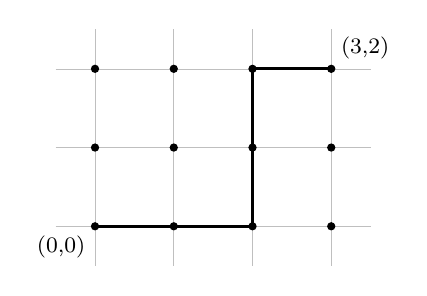
\begin{tikzpicture}
      \draw[very thin, color=gray!50] (-.5,-.5) grid (3.5, 2.5);
      \foreach \x in {0,...,3}
      \foreach \y in {0,...,2}
      \fill (\x,\y) circle (1.5pt);
      \draw (0,0) node[below left] {\footnotesize (0,0)} (3,2) node[above right] {\footnotesize (3,2)};
      \draw[very thick] (0,0) -- (2,0) -- (2,2) -- (3,2);
    \end{tikzpicture}

  \end{center}

  \begin{center}
    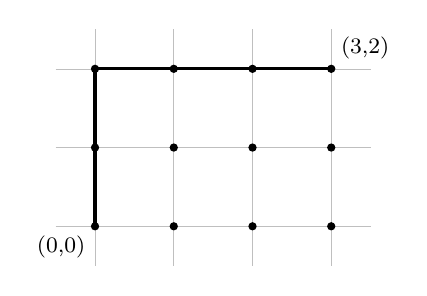
\begin{tikzpicture}
      \draw[very thin, color=gray!50] (-.5,-.5) grid (3.5, 2.5);
      \foreach \x in {0,...,3}
      \foreach \y in {0,...,2}
      \fill (\x,\y) circle (1.5pt);
      \draw (0,0) node[below left] {\footnotesize (0,0)} (3,2) node[above right] {\footnotesize (3,2)};
      \draw[very thick] (0,0) -- (0,2) -- (3,2);
    \end{tikzpicture}

  \end{center}

    \begin{center}
    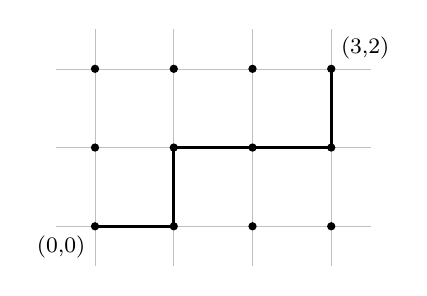
\begin{tikzpicture}
      \draw[very thin, color=gray!50] (-.5,-.5) grid (3.5, 2.5);
      \foreach \x in {0,...,3}
      \foreach \y in {0,...,2}
      \fill (\x,\y) circle (1.5pt);
      \draw (0,0) node[below left] {\footnotesize (0,0)} (3,2) node[above right] {\footnotesize (3,2)};
      \draw[very thick] (0,0) -- (1,0) -- (1,1) -- (3,1) -- (3,2);
    \end{tikzpicture}

  \end{center}
\end{multicols}

Notice to ensure the path is the {\em shortest} possible, each move must be either to the right or up.  Additionally, in this case, each path has {\em length} 5 as no matter what order we take them in, we must take three steps right and two steps up.

The counting question: how many lattice paths are there between $(0,0)$ and $(3,2)$?  We could try to draw all of these, or instead of drawing them, maybe just list which direction we travel on each of the 5 steps.  One path might be RRUUR, or maybe UURRR, or perhaps RURRU (those correspond to the three paths drawn above).  So how many such strings of R's and U's are there?

Notice that each of these strings must contain 5 symbols.  Exactly 3 of them must be R's (since our destination is 3 units to the right).  This seems awfully familiar.  In fact, what if we used $1$'s instead of R's and 0's instead of U's?  Then we would just have 5-bit strings of weight 3.  There are 10 of those, so there are 10 lattice paths from (0,0) to (3,2).

The correspondence between bit strings and lattice paths does not stop there.  Here is another way to count lattice paths.  Consider the lattice shown below:

  \begin{center}
    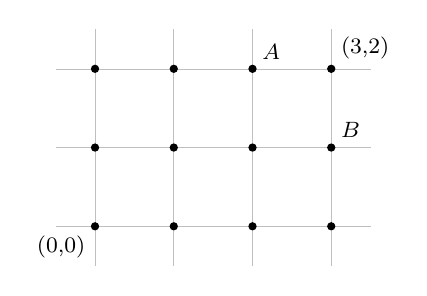
\begin{tikzpicture}
      \draw[very thin, color=gray!50] (-.5,-.5) grid (3.5, 2.5);
      \foreach \x in {0,...,3}
      \foreach \y in {0,...,2}
      \fill (\x,\y) circle (1.5pt);
      \draw (0,0) node[below left] {\footnotesize (0,0)} (3,2) node[above right] {\footnotesize (3,2)};
      \draw (3,1) node[above right] {\footnotesize $B$} (2,2) node[above right]{\footnotesize $A$};
    \end{tikzpicture}

  \end{center}

Any lattice path from (0,0) to (3,2) must pass through exactly one of $A$ and $B$.  The point $A$ is 4 steps away from (0,0) and two of them are right.  The number of lattice paths to $A$ is the same as the number of 4-bit strings of weight 2, namely 6.  The point $B$ is 4 steps away from (0,0), but now 3 of them are right.  So the number of paths to point $B$ is the same as the number of 4-bit strings of weight 3, namely 4.  So the total number of paths to (3,2) is just $6+4$.  This is the same way we calculated the number of 5-bit strings of weight 3.  The point: the exact same recurrence relation exists for bit strings and for lattice paths.


\subsubsection*{Binomial Coefficients}

Binomial coefficients are the coefficients in the expanded version of a binomial, such as $(x+y)^5$.  What happens when we multiply such a binomial out?  We will expand $(x+y)^n$ for various values of $n$.  Each of these are done by multiplying everything out (i.e., FOIL-ing) and then collecting like terms.

\[(x+y)^1 = x + y\]
\[(x+y)^2 = x^2 + 2xy + y^2\]
\[(x+y)^3 = x^3 + 3x^2y + 3xy^2 + y^3\]
\[(x+y)^4 = x^4 + 4x^3y + 6x^2y^2 + 4xy^3 + y^4.\]

In fact, there is a quicker way to expand the above binomials.  For example, consider the next one, $(x+y)^5$.  What we are really doing is multiplying out,
\[(x+y)(x+y)(x+y)(x+y)(x+y).\]
In the expansion, there will be only one $x^5$ term and one $y^5$ term.  This is because to get an $x^5$, we need to use the $x$ term in each of the copies of the binomial $(x+y)$, and similarly for $y^5$.  What about $x^4y$?  To get terms like this, we need to use four $x$'s and one $y$, so we need exactly one of the five binomials to contribute a $y$.  There are 5 choices for this, so there are 5 ways to get $x^4y$, so the coefficient of $x^4y$ is 5.  This is also the coefficient for $xy^4$ for the same (but opposite) reason: there are 5 ways to pick which of the 5 binomials contribute the single $x$.  So far we have
\[(x+y)^5 = x^5 + 5x^4y + \underline{~?~}~x^3y^2 + \underline{~?~}~x^2y^3 + 5 xy^4 + y^5.\]
We still need the coefficients of $x^3y^2$ and $x^2y^3$.  In both cases, we need to pick exactly 3 of the 5 binomials to contribute one variable, the other two to contribute the other.  Wait.  This sounds familiar.   We have 5 things, each can be one of two things, and we need a total of 3 of one of them.  That's just like taking 5 bits and making sure exactly 3 of them are 1's.  So the coefficient of $x^3y^2$ (and also $x^2y^3$) will be exactly the same as the number of bit strings of length 5 and weight 3, which we found earlier to be 10.  So we have:
\[(x+y)^5 = x^5 + 5x^4y + 10x^3y^2 + 10x^2y^3 + 5 xy^4 + y^5.\]

These numbers we keep seeing over and over again.  They are the number of subsets of a particular size, the number of bit strings of a particular weight, the number of lattice paths, and the coefficients of these binomial products.  We will call them {\em binomial coefficients}.  We even have a special symbol for them: ${n \choose k}$.

\begin{defbox}{Binomial Coefficients\index{binomial coefficients}}
  For each integer $n \ge 0$ and integer $k$ with $0 \le k \le n$ there is a number
  \[\gls{cnk} \]
  read ``$n$ choose $k$.''  We have:
  \begin{itemize}
    \item ${n\choose k} = |\b B^n_k|$, the number of $n$-bit strings of weight $k$.
    \item ${n \choose k}$ is the number of subsets of a set of size $n$ each with cardinality $k$.
    \item ${n \choose k}$ is the number of lattice paths of length $n$ containing $k$ steps to the right.
    \item ${n \choose k}$ is the coefficient of $x^ky^{n-k}$ in the expansion of $(x+y)^n$.
    \item ${n \choose k}$ is the number of ways to select $k$ objects from a total of $n$ objects.
  \end{itemize}
\end{defbox}

The last bullet point is usually taken as the definition of ${n \choose k}$.  Out of $n$ objects we must choose $k$ of them, so there are $n$ choose $k$ ways of doing this.  Each of our counting problems above can be viewed in this way:
\begin{itemize}
  \item How many subsets of $\{1,2,3,4,5\}$ contain exactly 3 elements?  We must choose $3$ of the 5 elements to be in our subset.  There are ${5 \choose 3}$ ways to do this, so there are ${5 \choose 3}$ such subsets.
  \item How many bit strings have length 5 and weight 3?  We must choose $3$ of the 5 bits to be 1's.  There are ${5 \choose 3}$ ways to do this, so there are ${5 \choose 3}$ such bit strings.
  \item How many lattice paths are there from (0,0) to (3,2)?  We must choose 3 of the 5 steps to be towards the right.  There are ${5 \choose 3}$ ways to do this, so there are ${5 \choose 3}$ such lattice paths.
  \item What is the coefficient of $x^3y^2$ in the expansion of $(x+y)^5$?  We must choose 3 of the 5 copies of the binomial to contribute an $x$.  There are ${5 \choose 3}$ ways to do this, so the coefficient is ${5 \choose 3}$.
\end{itemize}

It should be clear that in each case above, we have the right answer.  All we had to do is phrase the question correctly and it became obvious that ${5 \choose 3}$ is correct.  However, this does not tell us that the answer is in fact 10 in each case.  We will eventually find a formula for ${n \choose k}$, but for now, look back at how we arrived at the answer 10 in our counting problems above.  It all came down to bit strings, and we have a recurrence relation for bit strings:
\[|\b B^n_k| = |\b B^{n-1}_{k-1}| + |\b B^{n-1}_k|.\]
Remember, this is because we can start the bit string with either a 1 or a 0.  In both cases, we have $n-1$ more bits to pick.  The strings starting with 1 must contain $k-1$ more 1's, while the strings starting with 0 still need $k$ more 1's.

Since $|\b B^n_k| = {n \choose k}$, the same recurrence relation holds for binomial coefficients:

\begin{defbox}{Recurrence relation for ${n \choose k}$}
  \[{n \choose k} = {n-1 \choose k-1} + {n-1 \choose k}\]
\end{defbox}

\subsection{Pascal's Triangle}\label{subsec:Pascal}

Let's arrange the binomial coefficients ${n \choose k}$ into a triangle like follows:

\begin{center}
  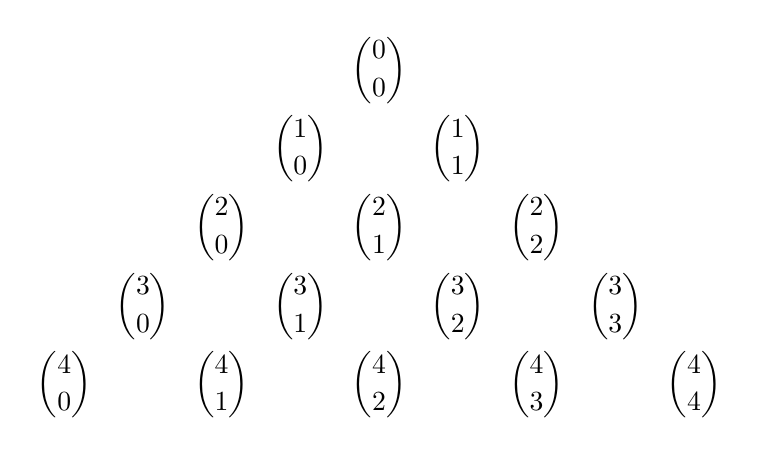
\begin{tikzpicture}
    \foreach \n in {0,...,4}
    \foreach \k in {0,...,\n}
    \draw (-\n+2*\k, -\n) node {$\displaystyle{\n \choose \k}$};
  \end{tikzpicture}

\end{center}

This can continue as far down as we like.  The recurrence relation for ${n \choose k}$ tells us that each entry in the triangle is the sum of the two entries above it.  The entries on the sides of the triangle are always 1.  This is because ${n \choose 0} = 1$ for all $n$ since there is only one way to pick 0 of $n$ objects and ${n \choose n} = 1$ since there is one way to select all $n$ out of $n$ objects.  Using the recurrence relation, and the fact that the sides of the triangle are 1's, we can easily replace all the entries above with the correct values of ${n \choose k}$.  Doing so gives us \emph{Pascal's triangle}.

We can use Pascal's triangle to calculate binomial coefficients.  For example, using the triangle on the next page, we can find ${12 \choose 6} = 924$.


\newpage
\thispagestyle{empty}
~
\vskip 1in
\begin{center}
\hspace*{-1.5em}{\Huge \textsc{Pascal's Triangle}\index{Pascal's triangle}}
\end{center}
\vskip 2cm
\hspace*{-1.5em}
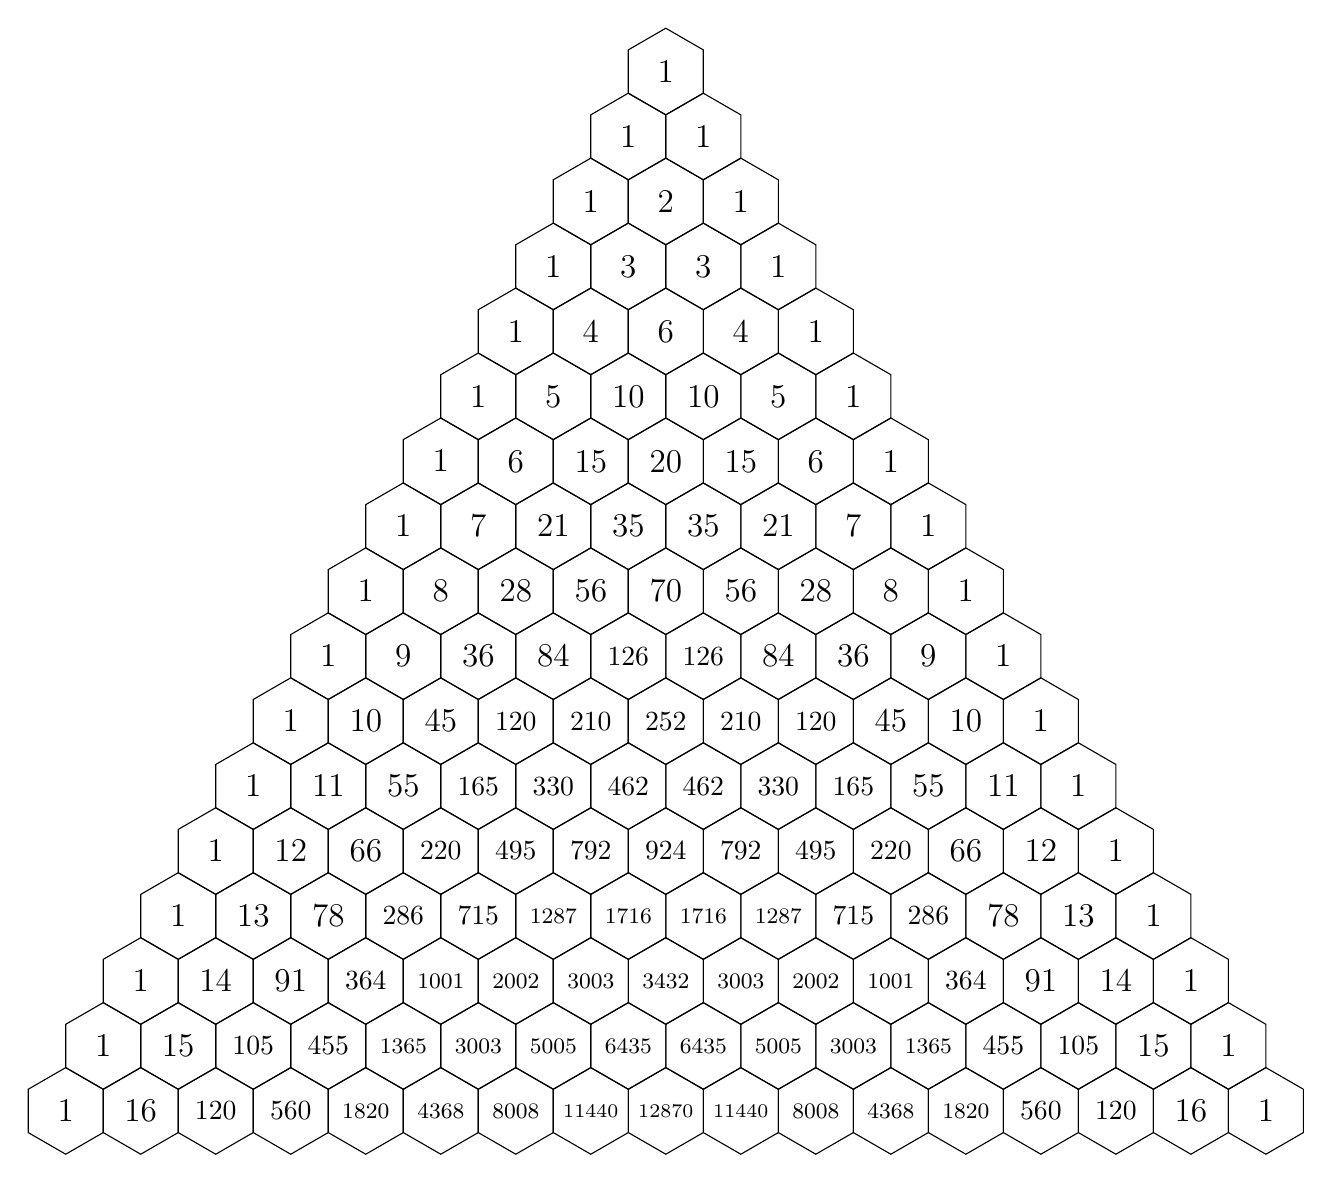
\begin{tikzpicture}
\def\r{.55}
\newcommand{\hexbox}[3]{
  \def\x{-cos{30}*\r*#1+cos{30}*#2*\r*2}
  \def\y{-\r*#1-sin{30}*\r*#1}
  \draw (\x,\y) +(90:\r) -- +(30:\r) -- +(-30:\r) -- +(-90:\r) -- +(-150:\r) -- +(150:\r) -- cycle;
  \draw (\x,\y) node{#3};
}


% Pascal's triangle
%put row of 1's down left side:
  \foreach \row in {0,...,16} {
    \hexbox{\row}{0}{\large 1}
  }
%fill in the rest of the triangle:
  \foreach \row in {1,...,16} {
    \pgfmathsetmacro{\entry}{1};
    \foreach \col in {1,...,\row} {
      % iterative formula : val = precval * (row-col+1)/col
      % (+ 0.5 to bypass rounding errors)
      \pgfmathtruncatemacro{\entry}{\entry*((\row-\col+1)/\col)+0.5};
      \global\let\entry=\entry
      \ifnum \entry<100
	\hexbox{\row}{\col}{\large \entry}
      \else \ifnum \entry<1000
	\hexbox{\row}{\col}{\entry}
      \else \ifnum \entry<10000
	\hexbox{\row}{\col}{\footnotesize \entry}
	\else
	\hexbox{\row}{\col}{\scriptsize \entry}
	\fi
      \fi
      \fi
    }
  }
\end{tikzpicture}

\newpage




\end{document}

	\withanswers\documentclass[12pt]{article}

\usepackage{discrete}

\def\thetitle{Introduction to Counting} % will be put in the center header on the first page only.
\def\lefthead{Math 228 Notes} % will be put in the left header
\def\righthead{Counting} % will be put in the right header


\begin{document}

\section{Binomial Coefficients}\label{sec:binom}

\begin{activity}

In Chess, a rook can move only in straight lines (not diagonally).  Fill in each square of the chess board below with the number of different shortest paths the rook, in the upper left corner, can take to get to that square.  For example, one square is already filled in. There are six different paths from the rook to the square: DDRR (down down right right), DRDR, DRRD, RDDR, RDRD and RRDD.

 \cbDefineNewPiece{white}{x}{$6$}{$6$}
 \centerline{\chessboard[smallboard, borderwidth=.5px, showmover=false, labelleft=false, labelbottom=false, color=blue, setpieces={ra8, xc6}, blackfieldcolor=gray, setfontcolors]}

\end{activity}

Here are some apparently different discrete objects we can count: subsets, bit strings, lattice paths, and binomial coefficients.  We will give an example of each type of counting problem (and say what these things even are).  As we will see, these counting problems are surprisingly similar.

\subsubsection*{Subsets}\label{subsec:subsets}

Subsets should be familiar, otherwise read over \Cref{sec:sets} again.  Suppose we look at the set $A = \{1,2,3,4,5\}$.  How many subsets of $A$ contain exactly 3 elements?

First, a simpler question.  How many subsets of $A$ are there total?  In other words, what is $|\pow(A)|$ (the cardinality of the power set of $A$)?  Think about how we would build a subset. We need to decide, for each of the elements of $A$, whether or not to include the element in our subset.  So we need to decide ``yes'' or ``no'' for the element 1.  And for each choice we make, we need to decide ``yes'' or ``no'' for the element 2.  And so on.  For each of the 5 elements, we have 2 choices.  Therefore the number of subsets is simply $2^5$ (by the multiplicative principle).

Of those 32 subsets, how many have 3 elements?  This is not obvious.  Note that we cannot just use the multiplicative principle.  Maybe we want to say we have 2 choices for the first element, 2 choices for the second, 2 choices for the third, and then only 1 choice for the other two.  But what if we said ``no'' to one of the first three elements?  Then we would have two choices for the 4th element.  What a mess!

Another (bad) idea: we need to pick three elements to be in our subset.  There are 5 elements to choose from.  So there are 5 choices for the first element, and for each of those 4 choices for the second, and then 3 for the third (last) element.  The multiplicative principle would say then that there are a total of $5 \cdot 4 \cdot 3 = 60$ ways to select the 3 element subset.  But this cannot be correct ($60 > 32$ for one thing).  One of the outcomes we would get from these choices would be the set $\{3,2,5\}$, by choosing the element 3 first, then the element 2, then the element 5.  Another outcome would be $\{5,2,3\}$ by choosing the element 5 first, then the element 2, then the element 3.  But these are the same set!  We can correct this by dividing the supposed 60 outcomes by the number of different outcomes which count as the same for each three elements. There happen to be 6 of these.  So we expect there to be 10 3-element subsets of $A$.

Is this right?  Well, we could list out all 10 of them, being very systematic in doing so, to make sure we don't miss any or list any twice.  Or we could try to count how many subsets of $A$ {\em don't} have 3 elements in them.  How many have no elements?  Just 1 (the empty set).  How many have 5?  Again, just 1.  These are the cases in which we say ``no'' to all elements, or ``yes'' to all elements.  Okay, what about the subsets which contain a single element?  There are 5 of these.  We must say ``yes'' to exactly one element, and there are 5 to choose from.  This is also the number of subsets containing 4 elements.  Those are the ones for which we must say ``no'' to exactly one element.

So far we have counted 12 of the 32 subsets.  We have not yet counted the subsets with cardinality 2 and with cardinality 3.  There are a total of 20 subsets left to split up between these two groups.  But the number of each must be the same!  If we say ``yes'' to exactly two elements, that can be accomplished in exactly the same number of ways as the number of ways we can say ``no'' to exactly two elements.  So the number of 2-element subsets is equal to the number of 3-element subsets.  Together there are 20 of these subsets, so 10 each.

\begin{center}
\begin{tabular}{l|c|c|c|c|c|c}
  Number of elements: & 0 & 1 & 2 & 3 & 4 & 5 \\ \hline
  Number of subsets: & 1 & 5 & 10 & 10 & 5 & 1
\end{tabular}
\end{center}


\subsubsection*{Bit Strings}\label{subsec:bitstrings}

``Bit'' is short for ``binary digit,'' so a bit string is a string of binary digits.  The binary digits are simply the numbers 0 and 1.  All of the following are bit strings:
\[1001 \quad 0 \quad 1111 \quad 1010101010\]
The number of bits (0's or 1's) in the string is the {\em length} of the string;  the strings above have lengths 4, 1, 4, and 10 respectively.  We also can ask how many of the bits are 1's.  The number of 1's in a bit string is the {\em weight} of the string; the weights of the above strings are 2, 0, 4, and 5 respectively.

\begin{defbox}{Bit Strings\index{bit string}}
  \begin{itemize}
    \item A $n$-bit string is a bit string of length $n$.  That is, it is a string containing $n$ symbols, each of which is a bit, either 0 or 1.
    \item The {\em weight}\index{weight, of a string} of a bit string is the number of 1's in it.
    \item \gls{Bn} is the {\em set} of all $n$-bit strings.
    \item \gls{Bnk} is the set of all $n$-bit strings of weight $k$.
  \end{itemize}
\end{defbox}

For example, the elements of the set $\b B^3_2$ are the bit strings 011, 101, and 110.  Those are the only strings containing three bits exactly two of which are 1's.

The counting questions: How many bit strings have length 5?  How many of those have weight 3?  In other words, we are asking for the cardinalities $|\b B^5|$ and $|\b B^5_3|$.

To find the number of 5-bit strings is straight forward.  We have 5 bits, and each can either be a 0 or a 1.  So there are 2 choices for the first bit, 2 choices for the second, and so on.  By the multiplicative principle, there are $2 \cdot 2 \cdot 2\cdot 2 \cdot 2 = 2^5 = 32$ such strings.

Finding the number of 5-bit strings of weight 3 is harder.  Think about how such a string could start.  The first bit must be either a 0 or a 1.  In the first case (the string starts with a 0), we must then decide on four more bits.  To have a total of three 1's, among those four remaining bits there must be three 1's.  In other words, we must include all 4-bit strings of weight 3.  In the second case (the string starts with a 1), we still have four bits to choose, but now only two of them can be 1's, so we should look at all the 4-bit strings of weight 2.  In other words:
\[|\b B^5_3| = |\b B^4_2| + |\b B^4_3|.\]
This is an example of a {\em recurrence relation}.  We represented one instance of our counting problem in terms of two simpler instances of the problem.  It holds because the strings in $\b B^5_3$ all have the form $1\b B^4_2$ (that is, a 1 followed by a string from $\b B^4_2$) or $0\b B^4_3$.  If only we knew the cardinalities of $\b B^4_2$ and $\b B^4_3$.  Repeating the same reasoning,
\[|\b B^4_2| = |\b B^3_1| + |\b B^3_2| \quad \mbox{and}\quad |\b B^4_3| = |\b B^3_2| + |\b B^3_3|.\]
We can keep going down, but this should be good enough. Both $\b B^3_1$ and $\b B^3_2$ contain 3 bit strings: we must pick one of the three bits to be a 1 (three ways to do that) or one of the three bits to be a 0 (three ways to do that).  Also, $\b B^3_3$ contains just one string: 111.  Thus $|\b B^4_2| = 6$ and $|\b B^4_3| = 4$, which puts $\b B^5_3$ at a total of 10 strings.

But wait -- 32 and 10 were the answers to the counting questions about subsets.  Coincidence?  Not at all.  Each bit string can be thought of as a {\em code} for a subset.  For the set $A = \{1,2,3,4,5\}$, we would use 5-bit strings, one bit for each element of $A$.  Each bit in the string is a 0 if its corresponding element of $A$ is not in the subset, and a 1 if the element of $A$ is in the subset.  Remember, deciding the subset amounted to a sequence of five yes/no votes for the elements of $A$.  Instead of yes, we put a 1; instead of no, we put a 0.

For example, the bit string $11001$ represents the subset $\{1,2,5\}$ since the first, second and fifth bits are 1's.  The subset $\{3,5\}$ would be coded by the string $00101$.  What we really have here is a bijection from $\pow(A)$ to $\b B^5$.

Now for a subset to contain exactly three elements, the corresponding bit string must contain exactly three 1's.  In other words, the weight must be 3.  Thus counting the number of 3-element subsets of $A$ is the same as counting the number 5-bit strings of weight 3.
%Add something about a function here?

\subsubsection*{Lattice Paths}

The \emph{integer lattice} is the set of all points in the Cartesian plane for which both the $x$ and $y$ coordinates are integers.  If you like to draw graphs on graph paper, the lattice is the set of all the intersections of the grid lines.

A {\em lattice path}\index{lattice path} is one of the shortest possible paths connecting two points on the lattice, moving only horizontally and vertically.  For example, here are three possible lattice paths from the points $(0,0)$ to $(3,2)$:

\begin{multicols}{3}
  \begin{center}
    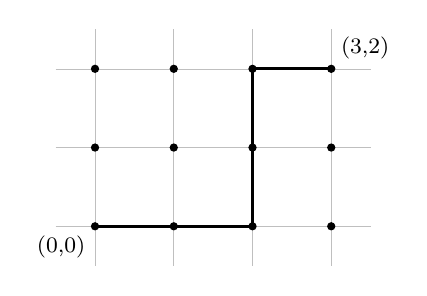
\begin{tikzpicture}
      \draw[very thin, color=gray!50] (-.5,-.5) grid (3.5, 2.5);
      \foreach \x in {0,...,3}
      \foreach \y in {0,...,2}
      \fill (\x,\y) circle (1.5pt);
      \draw (0,0) node[below left] {\footnotesize (0,0)} (3,2) node[above right] {\footnotesize (3,2)};
      \draw[very thick] (0,0) -- (2,0) -- (2,2) -- (3,2);
    \end{tikzpicture}

  \end{center}

  \begin{center}
    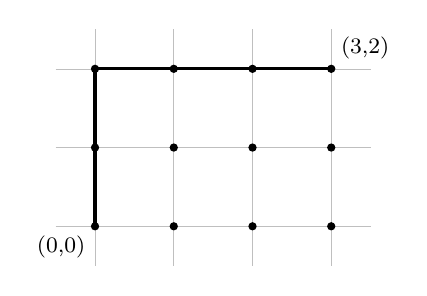
\begin{tikzpicture}
      \draw[very thin, color=gray!50] (-.5,-.5) grid (3.5, 2.5);
      \foreach \x in {0,...,3}
      \foreach \y in {0,...,2}
      \fill (\x,\y) circle (1.5pt);
      \draw (0,0) node[below left] {\footnotesize (0,0)} (3,2) node[above right] {\footnotesize (3,2)};
      \draw[very thick] (0,0) -- (0,2) -- (3,2);
    \end{tikzpicture}

  \end{center}

    \begin{center}
    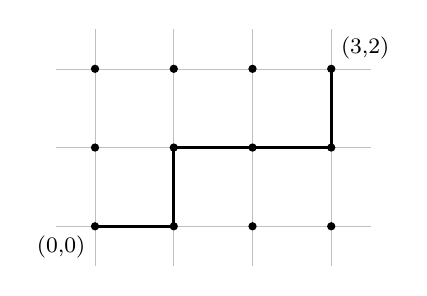
\begin{tikzpicture}
      \draw[very thin, color=gray!50] (-.5,-.5) grid (3.5, 2.5);
      \foreach \x in {0,...,3}
      \foreach \y in {0,...,2}
      \fill (\x,\y) circle (1.5pt);
      \draw (0,0) node[below left] {\footnotesize (0,0)} (3,2) node[above right] {\footnotesize (3,2)};
      \draw[very thick] (0,0) -- (1,0) -- (1,1) -- (3,1) -- (3,2);
    \end{tikzpicture}

  \end{center}
\end{multicols}

Notice to ensure the path is the {\em shortest} possible, each move must be either to the right or up.  Additionally, in this case, each path has {\em length} 5 as no matter what order we take them in, we must take three steps right and two steps up.

The counting question: how many lattice paths are there between $(0,0)$ and $(3,2)$?  We could try to draw all of these, or instead of drawing them, maybe just list which direction we travel on each of the 5 steps.  One path might be RRUUR, or maybe UURRR, or perhaps RURRU (those correspond to the three paths drawn above).  So how many such strings of R's and U's are there?

Notice that each of these strings must contain 5 symbols.  Exactly 3 of them must be R's (since our destination is 3 units to the right).  This seems awfully familiar.  In fact, what if we used $1$'s instead of R's and 0's instead of U's?  Then we would just have 5-bit strings of weight 3.  There are 10 of those, so there are 10 lattice paths from (0,0) to (3,2).

The correspondence between bit strings and lattice paths does not stop there.  Here is another way to count lattice paths.  Consider the lattice shown below:

  \begin{center}
    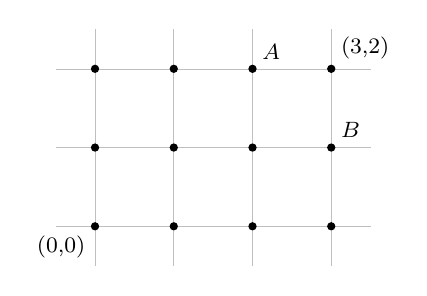
\begin{tikzpicture}
      \draw[very thin, color=gray!50] (-.5,-.5) grid (3.5, 2.5);
      \foreach \x in {0,...,3}
      \foreach \y in {0,...,2}
      \fill (\x,\y) circle (1.5pt);
      \draw (0,0) node[below left] {\footnotesize (0,0)} (3,2) node[above right] {\footnotesize (3,2)};
      \draw (3,1) node[above right] {\footnotesize $B$} (2,2) node[above right]{\footnotesize $A$};
    \end{tikzpicture}

  \end{center}

Any lattice path from (0,0) to (3,2) must pass through exactly one of $A$ and $B$.  The point $A$ is 4 steps away from (0,0) and two of them are right.  The number of lattice paths to $A$ is the same as the number of 4-bit strings of weight 2, namely 6.  The point $B$ is 4 steps away from (0,0), but now 3 of them are right.  So the number of paths to point $B$ is the same as the number of 4-bit strings of weight 3, namely 4.  So the total number of paths to (3,2) is just $6+4$.  This is the same way we calculated the number of 5-bit strings of weight 3.  The point: the exact same recurrence relation exists for bit strings and for lattice paths.


\subsubsection*{Binomial Coefficients}

Binomial coefficients are the coefficients in the expanded version of a binomial, such as $(x+y)^5$.  What happens when we multiply such a binomial out?  We will expand $(x+y)^n$ for various values of $n$.  Each of these are done by multiplying everything out (i.e., FOIL-ing) and then collecting like terms.

\[(x+y)^1 = x + y\]
\[(x+y)^2 = x^2 + 2xy + y^2\]
\[(x+y)^3 = x^3 + 3x^2y + 3xy^2 + y^3\]
\[(x+y)^4 = x^4 + 4x^3y + 6x^2y^2 + 4xy^3 + y^4.\]

In fact, there is a quicker way to expand the above binomials.  For example, consider the next one, $(x+y)^5$.  What we are really doing is multiplying out,
\[(x+y)(x+y)(x+y)(x+y)(x+y).\]
In the expansion, there will be only one $x^5$ term and one $y^5$ term.  This is because to get an $x^5$, we need to use the $x$ term in each of the copies of the binomial $(x+y)$, and similarly for $y^5$.  What about $x^4y$?  To get terms like this, we need to use four $x$'s and one $y$, so we need exactly one of the five binomials to contribute a $y$.  There are 5 choices for this, so there are 5 ways to get $x^4y$, so the coefficient of $x^4y$ is 5.  This is also the coefficient for $xy^4$ for the same (but opposite) reason: there are 5 ways to pick which of the 5 binomials contribute the single $x$.  So far we have
\[(x+y)^5 = x^5 + 5x^4y + \underline{~?~}~x^3y^2 + \underline{~?~}~x^2y^3 + 5 xy^4 + y^5.\]
We still need the coefficients of $x^3y^2$ and $x^2y^3$.  In both cases, we need to pick exactly 3 of the 5 binomials to contribute one variable, the other two to contribute the other.  Wait.  This sounds familiar.   We have 5 things, each can be one of two things, and we need a total of 3 of one of them.  That's just like taking 5 bits and making sure exactly 3 of them are 1's.  So the coefficient of $x^3y^2$ (and also $x^2y^3$) will be exactly the same as the number of bit strings of length 5 and weight 3, which we found earlier to be 10.  So we have:
\[(x+y)^5 = x^5 + 5x^4y + 10x^3y^2 + 10x^2y^3 + 5 xy^4 + y^5.\]

These numbers we keep seeing over and over again.  They are the number of subsets of a particular size, the number of bit strings of a particular weight, the number of lattice paths, and the coefficients of these binomial products.  We will call them {\em binomial coefficients}.  We even have a special symbol for them: ${n \choose k}$.

\begin{defbox}{Binomial Coefficients\index{binomial coefficients}}
  For each integer $n \ge 0$ and integer $k$ with $0 \le k \le n$ there is a number
  \[\gls{cnk} \]
  read ``$n$ choose $k$.''  We have:
  \begin{itemize}
    \item ${n\choose k} = |\b B^n_k|$, the number of $n$-bit strings of weight $k$.
    \item ${n \choose k}$ is the number of subsets of a set of size $n$ each with cardinality $k$.
    \item ${n \choose k}$ is the number of lattice paths of length $n$ containing $k$ steps to the right.
    \item ${n \choose k}$ is the coefficient of $x^ky^{n-k}$ in the expansion of $(x+y)^n$.
    \item ${n \choose k}$ is the number of ways to select $k$ objects from a total of $n$ objects.
  \end{itemize}
\end{defbox}

The last bullet point is usually taken as the definition of ${n \choose k}$.  Out of $n$ objects we must choose $k$ of them, so there are $n$ choose $k$ ways of doing this.  Each of our counting problems above can be viewed in this way:
\begin{itemize}
  \item How many subsets of $\{1,2,3,4,5\}$ contain exactly 3 elements?  We must choose $3$ of the 5 elements to be in our subset.  There are ${5 \choose 3}$ ways to do this, so there are ${5 \choose 3}$ such subsets.
  \item How many bit strings have length 5 and weight 3?  We must choose $3$ of the 5 bits to be 1's.  There are ${5 \choose 3}$ ways to do this, so there are ${5 \choose 3}$ such bit strings.
  \item How many lattice paths are there from (0,0) to (3,2)?  We must choose 3 of the 5 steps to be towards the right.  There are ${5 \choose 3}$ ways to do this, so there are ${5 \choose 3}$ such lattice paths.
  \item What is the coefficient of $x^3y^2$ in the expansion of $(x+y)^5$?  We must choose 3 of the 5 copies of the binomial to contribute an $x$.  There are ${5 \choose 3}$ ways to do this, so the coefficient is ${5 \choose 3}$.
\end{itemize}

It should be clear that in each case above, we have the right answer.  All we had to do is phrase the question correctly and it became obvious that ${5 \choose 3}$ is correct.  However, this does not tell us that the answer is in fact 10 in each case.  We will eventually find a formula for ${n \choose k}$, but for now, look back at how we arrived at the answer 10 in our counting problems above.  It all came down to bit strings, and we have a recurrence relation for bit strings:
\[|\b B^n_k| = |\b B^{n-1}_{k-1}| + |\b B^{n-1}_k|.\]
Remember, this is because we can start the bit string with either a 1 or a 0.  In both cases, we have $n-1$ more bits to pick.  The strings starting with 1 must contain $k-1$ more 1's, while the strings starting with 0 still need $k$ more 1's.

Since $|\b B^n_k| = {n \choose k}$, the same recurrence relation holds for binomial coefficients:

\begin{defbox}{Recurrence relation for ${n \choose k}$}
  \[{n \choose k} = {n-1 \choose k-1} + {n-1 \choose k}\]
\end{defbox}

\subsection{Pascal's Triangle}\label{subsec:Pascal}

Let's arrange the binomial coefficients ${n \choose k}$ into a triangle like follows:

\begin{center}
  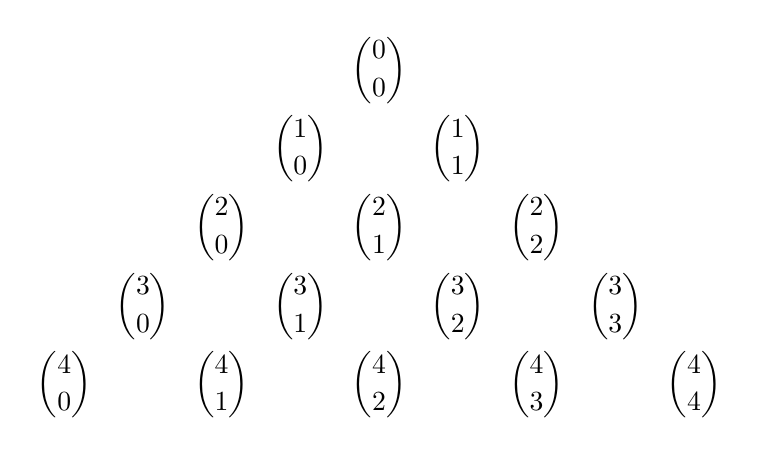
\begin{tikzpicture}
    \foreach \n in {0,...,4}
    \foreach \k in {0,...,\n}
    \draw (-\n+2*\k, -\n) node {$\displaystyle{\n \choose \k}$};
  \end{tikzpicture}

\end{center}

This can continue as far down as we like.  The recurrence relation for ${n \choose k}$ tells us that each entry in the triangle is the sum of the two entries above it.  The entries on the sides of the triangle are always 1.  This is because ${n \choose 0} = 1$ for all $n$ since there is only one way to pick 0 of $n$ objects and ${n \choose n} = 1$ since there is one way to select all $n$ out of $n$ objects.  Using the recurrence relation, and the fact that the sides of the triangle are 1's, we can easily replace all the entries above with the correct values of ${n \choose k}$.  Doing so gives us \emph{Pascal's triangle}.

We can use Pascal's triangle to calculate binomial coefficients.  For example, using the triangle on the next page, we can find ${12 \choose 6} = 924$.


\newpage
\thispagestyle{empty}
~
\vskip 1in
\begin{center}
\hspace*{-1.5em}{\Huge \textsc{Pascal's Triangle}\index{Pascal's triangle}}
\end{center}
\vskip 2cm
\hspace*{-1.5em}
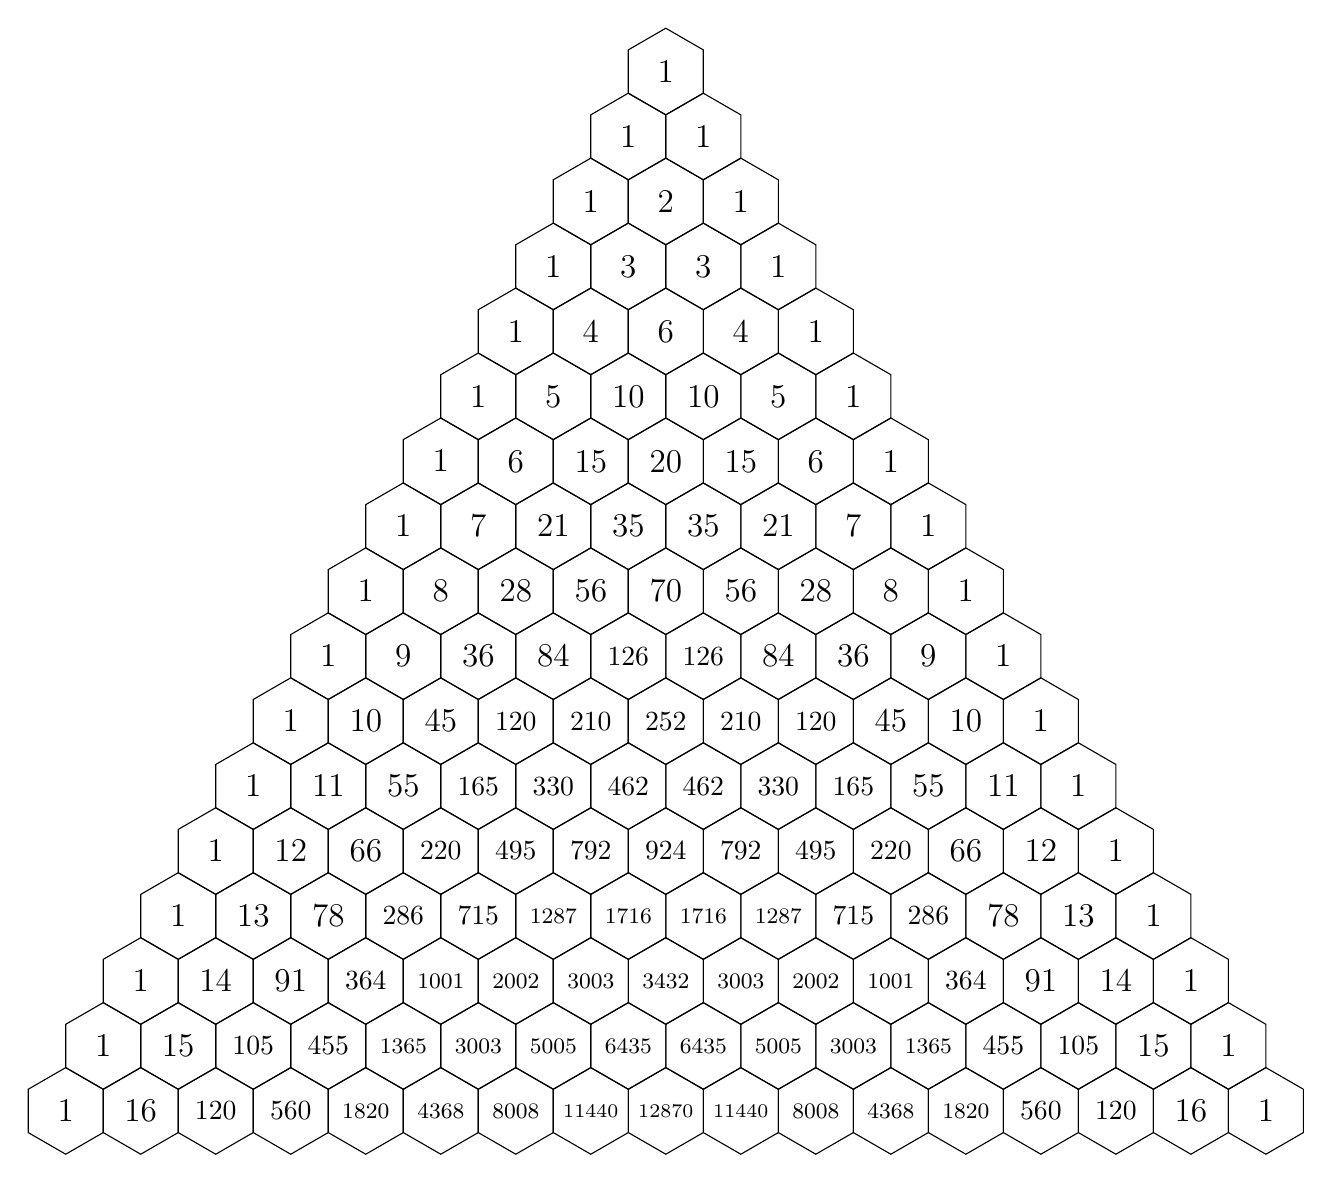
\begin{tikzpicture}
\def\r{.55}
\newcommand{\hexbox}[3]{
  \def\x{-cos{30}*\r*#1+cos{30}*#2*\r*2}
  \def\y{-\r*#1-sin{30}*\r*#1}
  \draw (\x,\y) +(90:\r) -- +(30:\r) -- +(-30:\r) -- +(-90:\r) -- +(-150:\r) -- +(150:\r) -- cycle;
  \draw (\x,\y) node{#3};
}


% Pascal's triangle
%put row of 1's down left side:
  \foreach \row in {0,...,16} {
    \hexbox{\row}{0}{\large 1}
  }
%fill in the rest of the triangle:
  \foreach \row in {1,...,16} {
    \pgfmathsetmacro{\entry}{1};
    \foreach \col in {1,...,\row} {
      % iterative formula : val = precval * (row-col+1)/col
      % (+ 0.5 to bypass rounding errors)
      \pgfmathtruncatemacro{\entry}{\entry*((\row-\col+1)/\col)+0.5};
      \global\let\entry=\entry
      \ifnum \entry<100
	\hexbox{\row}{\col}{\large \entry}
      \else \ifnum \entry<1000
	\hexbox{\row}{\col}{\entry}
      \else \ifnum \entry<10000
	\hexbox{\row}{\col}{\footnotesize \entry}
	\else
	\hexbox{\row}{\col}{\scriptsize \entry}
	\fi
      \fi
      \fi
    }
  }
\end{tikzpicture}

\newpage




\end{document}


	\input{chapters/Counting-CombinationsPermutations}
	\withanswers\input{exercises/Counting-CombinationsPermutations}

	\documentclass[12pt]{article}

\usepackage{discrete}

\def\thetitle{Combinatorial Proofs} % will be put in the center header on the first page only.
\def\lefthead{Math 228 Notes} % will be put in the left header
\def\righthead{\thetitle} % will be put in the right header





\begin{document}
\newpage
\section{Combinatorial Proofs}\label{sec:comb-proofs}

\begin{activity}
\begin{questions}
\question The Stanley Cup is decided in a best of 7 tournament between two teams.  In how many ways can your team win?  Let's answer this question two ways:
\begin{parts}
  \part How many of the 7 games does your team need to win?  How many ways can this happen?
  \part What if the tournament goes all 7 games?  So you win the last game.  How many ways can the first 6 games go down?
  \part What if the tournament goes just 6 games?  How many ways can this happen?  What about 5 games?  4 games?
  \part What are the two different ways to compute the number of ways your team can win?  Write down an equation involving binary coefficients (that is, ${n \choose k}$'s).  What pattern in Pascal's triangle is this an example of?
\end{parts}
\question Generalize.  What if the rules changed and you played a best of $9$ tournament (5 wins required)?  What if you played an $n$ game tournament with $k$ wins required to be named champion?
\end{questions}

\end{activity}



\subsection{Patterns in Pascal's Triangle}\label{subsec:patternsPascal}

Have a look again at Pascal's triangle.  Forget for a moment where it comes from - just look at it as a mathematical object.  What do you notice?

\begin{center}
\noindent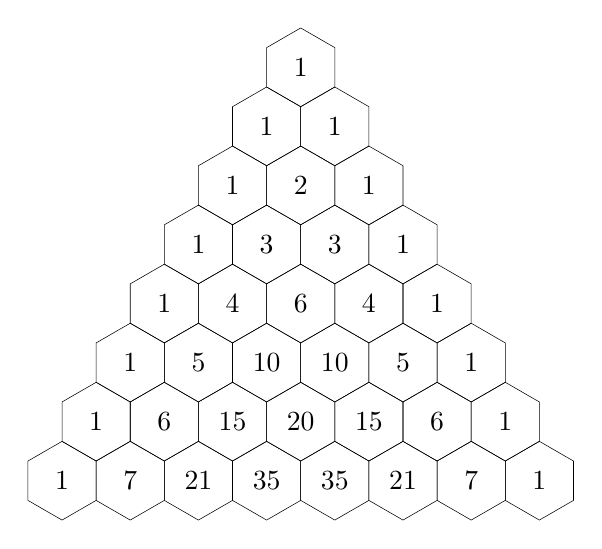
\begin{tikzpicture}
\def\r{.5}
\newcommand{\hexbox}[3]{
  \def\x{-cos{30}*\r*#1+cos{30}*#2*\r*2}
  \def\y{-\r*#1-sin{30}*\r*#1}
  \draw[very thin] (\x,\y) +(90:\r) -- +(30:\r) -- +(-30:\r) -- +(-90:\r) -- +(-150:\r) -- +(150:\r) -- cycle;
  \draw (\x,\y) node{ #3};
}


% Pascal's triangle
%put row of 1's down left side:
  \foreach \row in {0,...,7} {
    \hexbox{\row}{0}{ 1}
  }
%fill in the rest of the triangle:
  \foreach \row in {1,...,7} {
    \pgfmathsetmacro{\entry}{1};
    \foreach \col in {1,...,\row} {
      % iterative formula : val = precval * (row-col+1)/col
      % (+ 0.5 to bypass rounding errors)
     \pgfmathtruncatemacro{\entry}{\entry*((\row-\col+1)/\col)+0.5};
      \global\let\entry=\entry
      \ifnum \entry<100
	\hexbox{\row}{\col}{\entry}
      \else \ifnum \entry<1000
	\hexbox{\row}{\col}{\footnotesize \entry}
      \else \ifnum \entry<10000
	\hexbox{\row}{\col}{\footnotesize \entry}
	\else
	\hexbox{\row}{\col}{\scriptsize \entry}
	\fi
      \fi
      \fi
    }
  }
\end{tikzpicture}

\end{center}

There are lots of patterns hidden away in the triangle, enough to fill a reasonably sized book.  Here are just a few of the most obvious ones:
\begin{enumerate}
  \item The entries on the border of the triangle are all 1.
  \item Any entry not on the border is the sum of the two entries above it.
  \item The triangle is symmetric.  On any row, entries on the left side are mirrored on the right side.
  \item The sum of all entries on a given row is a power of 2. (You should check this!)
\end{enumerate}

We would like to state these observations in a more precise way, and then prove that they are correct.  Now each entry in Pascal's triangle is in fact a binomial coefficient.  The 1 on the very top of the triangle is ${0 \choose 0}$.  The next row (which we will call row 1, even though it is not the top-most row) consists of ${1 \choose 0}$ and ${1 \choose 1}$.  Row 4 (the row 1, 4, 6, 4, 1) consists of the binomial coefficients
\[{4 \choose 0} ~~ {4 \choose 1} ~~ {4 \choose 2} ~~ {4 \choose 3} ~~ {4 \choose 4}.\]
Given this description of the elements in Pascal's triangle, we can rewrite the above observations as follows:
\begin{enumerate}
  \item ${n \choose 0} = 1$ and ${n \choose n} = 1$.
  \item ${n \choose k} = {n-1 \choose k-1} + {n-1 \choose k}$.
  \item ${n \choose k} = {n \choose n-k}$.
  \item ${n\choose 0} + {n \choose 1} + {n \choose 2} + \cdots + {n \choose n} = 2^n$.
\end{enumerate}

Each of these are an example of a {\em binomial identity}\index{binomial identity}: an identity (i.e., equation) involving binomial coefficients.

Our goal is to establish these identities.  We wish to prove that they hold for all values of $n$ and $k$.  These proofs can be done in many ways.  One option would be to give algebraic proofs, using the formula for ${n \choose k}$:
\[{n \choose k} = \frac{n!}{(n-k)!\,k!}.\]
Here's how you might do that for the second identity above.

\begin{example}
  Give an algebraic proof for the binomial identity
  \[{n \choose k} = {n-1\choose k-1} + {n-1 \choose k}.\]
  \begin{proof}
    By the definition of ${n \choose k}$, we have
    \[{n-1 \choose k-1} = \frac{(n-1)!}{(n-1-(k-1))!(k-1)!} = \frac{(n-1)!}{(n-k)!(k-1)!} \hfill \mbox{ and } {n-1 \choose k} = \frac{(n-1)!}{(n-1-k)!k!}.\]
    Thus, starting with the right hand side of the equation we are trying to establish:
    \begin{align*}
      {n-1 \choose k-1} + {n-1 \choose k} & = \frac{(n-1)!}{(n-k)!(k-1)!}+ \frac{(n-1)!}{(n-1-k)!\,k!}\\
      & = \frac{(n-1)!k}{(n-k)!\,k!} + \frac{(n-1)!(n-k)}{(n-k)!\,k!}\\
      & = \frac{(n-1)!(k+n-k)}{(n-k)!\,k!} \\
      & = \frac{n!}{(n-k)!\, k!} \\
      & = {n \choose k}.
    \end{align*}
    The second line (where the common denominator is found) works because $k(k-1)! = k!$ and $(n-k)(n-k-1)! = (n-k)!$.
  \end{proof}

\end{example}

This is certainly a valid proof, but also is entirely useless.  Even if you understand the proof perfectly, it does not tell you {\em why} the identity is true.  A better approach would be to explain what ${n \choose k}$ {\em means} and then say why that is also what ${n-1 \choose k-1} + {n-1 \choose k}$ means.  Let's see how this works for the four identities we observed above.

\begin{example}
  Explain why ${n \choose 0} = 1$ and ${n \choose n} = 1$.
  \begin{solution}
    What do these binomial coefficients tell us? Well, ${n \choose 0}$ gives the number of ways to select 0 objects from a collection of $n$ objects.  There is only one way to do this, namely to not select any of the objects.  Thus ${n \choose 0} = 1$.  Similarly, ${n \choose n}$ gives the number of ways to select $n$ objects from a collection of $n$ objects.  There is only one way to do this: select all $n$ objects.  Thus ${n \choose n} = 1$.

    Alternatively, we know that ${n \choose 0}$ is the number of $n$-bit strings with weight 0.  There is only one such string, the string of all 0's.  So ${n \choose 0} = 1$.  Similarly ${n \choose n}$ is the number of $n$-bit strings with weight $n$.  There is only one string with this property, the string of all 1's.

    Another way: ${n \choose 0}$ gives the number of subsets of a set of size $n$ containing 0 elements.  There is only one such subset, the empty set.  ${n \choose n}$ gives the number of subsets containing $n$ elements.  The only such subset is the original set (of all elements).
  \end{solution}

\end{example}

\begin{example}
  Explain why ${n \choose k} = {n-1 \choose k-1} + {n-1 \choose k}$.
  \begin{solution}
    The easiest way to see this is to consider bit strings.  ${n \choose k}$ is the number of bit strings of length $n$ containing $k$ 1's.  Of all of these strings, some start with a 1 and the rest start with a 0.  First consider all the bit strings which start with a 1.  After the 1, there must be $n-1$ more bits (to get the total length up to $n$) and exactly $k-1$ of them must be 1's (as we already have one, and we need $k$ total).  How many strings are there like that?  There are exactly ${n-1 \choose k-1}$ such bit strings, so of all the length $n$ bit strings containing $k$ 1's, ${n-1 \choose k-1}$ of them start with a 1.  Similarly, there are ${n-1\choose k}$ which start with a 0 (we still need $n-1$ bits and now $k$ of them must be 1's).  Since there are ${n-1 \choose k}$ bit strings containing $n-1$ bits with $k$ 1's, that is the number of length $n$ bit strings with $k$ 1's which start with a 0.

    Another way: consider the question, how many ways can you select $k$ pizza toppings from a menu containing $n$ choices?  One way to do this is just ${n \choose k}$.  Another way to answer the same question is to first decide whether or not you want anchovies.  If you do want anchovies, you still need to pick $k-1$ toppings, now from just $n-1$ choices.  That can be done in ${n-1 \choose k-1}$ ways.  If you do not want anchovies, then you still need to select $k$ toppings from $n-1$ choices (the anchovies are out).  You can do that in ${n-1 \choose k}$ ways.  Since the choices with anchovies are disjoint from the choices without anchovies, the total choices are ${n-1 \choose k-1}+{n-1 \choose k}$.  But wait.  We answered the same question in two different ways, so the two answers must be the same.  Thus ${n \choose k} = {n-1\choose k-1} + {n-1 \choose k}$.

    You can also explain (prove) this identity by counting subsets, or even lattice paths.
  \end{solution}

\end{example}


\begin{example}
  Prove the binomial identity ${n \choose k} = {n \choose n-k}$.
  \begin{solution}
    Why is this true?  ${n \choose k}$ counts the number of ways to select $k$ things from $n$ choices.  On the other hand, ${n \choose n-k}$ counts the number of ways to select $n-k$ things from $n$ choices.  Are these really the same?  Well, what if instead of selecting the $n-k$ things you choose to exclude them.  How many ways are there to choose $n-k$ things to exclude from $n$ choices.  Clearly this is ${n \choose n-k}$ as well (it doesn't matter whether you include or exclude the things once you have chosen them).  And if you exclude $n-k$ things, then you are including the other $k$ things.  So the set of outcomes should be the same.

    Let's try the pizza counting example like we did above.  How many ways are there to pick $k$ toppings from a list of $n$ choices?  On the one hand, the answer is simply ${n \choose k}$.  Alternatively, you could make a list of all the toppings you don't want.  To end up with a pizza containing exactly $k$ toppings, you need to pick $n-k$ toppings to not put on the pizza.  You have ${n \choose n-k}$ choices for the toppings you don't want. Both of these ways give you a pizza with $k$ toppings, in fact all the ways to get a pizza with $k$ toppings.  Thus  these two answers must be the same: ${n \choose k} = {n \choose n-k}$.

    You can also prove (explain) this identity using bit strings, subsets, or lattice paths.  The bit string argument is nice: ${n \choose k}$ counts the number of bit strings of length $n$ with $k$ 1's.  This is also the number of bit string of length $n$ with $k$ 0's (just replace each 1 with a 0 and each 0 with a 1).  But if a string of length $n$ has $k$ 0's, it must have $n-k$ 1's.  And there are exactly ${n\choose n-k}$ strings of length $n$ with $n-k$ 1's.
  \end{solution}
\end{example}

\begin{example}
  Prove the binomial identity ${n\choose 0} + {n \choose 1} + {n\choose 2} + \cdots + {n \choose n} = 2^n$.
  \begin{solution}
    Let's do a ``pizza proof'' again.  We need to find a question about pizza toppings which has $2^n$ as the answer.  How about this: If a pizza joint offers $n$ toppings, how many pizzas can you build using any number of toppings from no toppings to all toppings, using each topping at most once?

    On one hand, the answer is $2^n$.  For each topping you can say ``yes'' or ``no,'' so you have two choices for each topping.

    On the other hand, divide the possible pizzas into disjoint groups: the pizzas with no toppings, the pizzas with one topping, the pizzas with two toppings, etc.  If we want no toppings, there is only one pizza like that (the empty pizza, if you will) but it would be better to think of that number as ${n \choose 0}$ since we choose 0 of the $n$ toppings.  How many pizzas have 1 topping?  We need to choose 1 of the $n$ toppings, so ${n \choose 1}$.  We have:
    \begin{itemize}
      \item[] Pizzas with 0 toppings: ${n \choose 0}$
      \item[] Pizzas with 1 topping: ${n \choose 1}$
      \item[] Pizzas with 2 toppings: ${n \choose 2}$
      \item[] \qquad $\vdots$
      \item[] Pizzas with $n$ toppings: ${n \choose n}$.
    \end{itemize}
    The total number of possible pizzas will be the sum of these, which is exactly the left hand side of the identity we are trying to prove.

    Again, we could have proved the identity using subsets, bit strings, or lattice paths (although the lattice path argument is a little tricky).
  \end{solution}

\end{example}

Hopefully this gives some idea of how explanatory proofs of binomial identities can go.  It is worth pointing out that sometimes more traditional proofs are also nice.\footnote{Most every binomial identity can be proved using mathematical induction, using the recursive definition for ${n \choose k}$.  We will discuss induction in \Cref{sec:induction}.}  For example, consider the following rather slick proof of the last identity.

Recall the binomial theorem:
\[(x + y)^n = {n \choose 0}x^n + {n \choose 1}x^{n-1}y + {n \choose 2}x^{n-2}y^2 + \cdots + {n \choose n-1}x\cdot y^n + {n \choose n}y^n.\]
Let $x = 1$ and $y = 1$.  We get:
\[(1 + 1)^n = {n \choose 0}1^n + {n \choose 1}1^{n-1}1 + {n \choose 2}1^{n-2}1^2 + \cdots + {n \choose n-1}1\cdot 1^n + {n \choose n}1^n.\]
Of course this simplifies to:
\[(2)^n = {n \choose 0} + {n \choose 1} + {n \choose 2} + \cdots + {n \choose n-1} + {n \choose n}.\]
Something fun to try: Let $x = 1$ and $y = 2$.  Neat huh?

\subsection{More Proofs}\label{subsec:moreProofs}

The explanatory proofs given in the above examples are typically called {\em combinatorial proofs}.  In general, to give a combinatorial proof for a binomial identity, say $A = B$ you do the following:
\begin{enumerate}
  \item Find a counting problem you will be able to answer in two ways.
  \item Explain why one answer to the counting problem is $A$.
  \item Explain why the other answer to the counting problem is $B$.
\end{enumerate}

Since both $A$ and $B$ are the answers to the same question, we must have $A = B$.

The tricky thing is coming up with the question.  This is not always obvious, but it gets easier the more counting problems you solve.  You will start to recognize types of answers as the answers to types of questions.  More often what will happen is you will be solving a counting problem and happen to think up two different ways of finding the answer.  Now you have a binomial identity and the proof is right there.  The proof \emph{is} the problem you just solved together with your two solutions.

For example, consider this counting question:

\begin{quote}
  How many 10-letter words use exactly four A's, three B's, two C's and one D?
\end{quote}

Let's try to solve this problem.  We have 10 spots for letters to go.  Four of those need to be A's.  We can pick the four A-spots in ${10 \choose 4}$ ways.  Now where can we put the B's?  Well there are only 6 spots left, we need to pick $3$ of them.  This can be done in ${6 \choose 3}$ ways.  The two C's need to go in two of the 3 remaining spots, so we have ${3 \choose 2}$ ways of doing that.  That leaves just one spot of the D, but we could write that 1 choice as ${1 \choose 1}$.  Thus the answer is:
\[{10 \choose 4}{6 \choose 3}{3 \choose 2}{1 \choose 1}.\]
But why stop there?  We can find the answer another way too.  First let's decide where to put the one D: we have 10 spots, we need to choose 1 of them, so this can be done in ${10 \choose 1}$ ways.  Next, choose one of the ${9 \choose 2}$ ways to place the two C's.  We now have $7$ spots left, and three of them need to be filled with B's.  There are ${7 \choose 3}$ ways to do this.  Finally the A's can be placed in ${4 \choose 4}$ (that is, only one) ways.  So another answer to the question is
\[{10 \choose 1}{9 \choose 2}{7 \choose 3}{4 \choose 4}.\]
Interesting.  This gives us the binomial identity:
\[{10 \choose 4}{6 \choose 3}{3 \choose 2}{1 \choose 1} = {10 \choose 1}{9 \choose 2}{7 \choose 3}{4 \choose 4}.\]
Here are a couple of other binomial identities with combinatorial proofs.

\begin{example}
  Prove the identity
  \[1 n + 2(n-1) + 3  (n-2) + \cdots + (n-1) 2 + n  1 = {n+2 \choose 3}.\]
  \begin{solution}
    To give a combinatorial proof we need to think up a question we can answer in two ways: one way needs to give the left-hand-side of the identity, the other way needs to be the right-hand-side of the identity.  Our clue to what question to ask comes from the right hand side: ${n+2 \choose 3}$ counts the number of ways to select 3 things from a group of $n+2$ things.  Let's name those things $1, 2, 3, \ldots, n+2$.  In other words, we want to find 3-element subsets of those numbers (since order should not matter, subsets are exactly the right thing to think about).  We will have to be a bit clever to explain why the left-hand-side also gives the number of these subsets.  Here's the proof.

    \begin{proof}
      Consider the question ``How many 3-element subsets are there of the set $\{1,2,3,\ldots, n+2\}$?''  We answer this in two ways:

      \underline{Answer 1}: We must select 3 elements from the collection of $n+2$ elements.  This can be done in ${n+2 \choose 3}$ ways.

      \underline{Answer 2}: Break this problem up into cases by what the middle number in the subset is.  Say each subset is $\{a,b,c\}$ written in increasing order.  We count the number of subsets for each distinct value of $b$.  The smallest possible value of $b$ is $2$, and the largest is $n+1$.

      When $b = 2$, there are $1 \cdot n$ subsets: 1 choice for $a$ and $n$ choices (3 through $n+2$) for $c$.

      When $b = 3$, there are $2 \cdot (n-1)$ subsets: 2 choices for $a$ and $n-1$ choices for $c$.

      When $b = 4$, there are $3 \cdot (n-2)$ subsets: 3 choices for $a$ and $n-2$ choices for $c$.

      And so on.  When $b = n+1$, there are $n$ choices for $a$ and only 1 choice for $c$, so $n \cdot 1$ subsets.

      Therefore the total number of subsets is \[1 n + 2 (n-1) + 3  (n-2) + \cdots + (n-1)2 + n  1.\]

      Since Answer 1 and Answer 2 are answers to the same question, they must be equal.  Therefore
      \[1 n + 2 (n-1) + 3  (n-2) + \cdots + (n-1) 2 + n  1 = {n+2 \choose 3}.\]

    \end{proof}

  \end{solution}

\end{example}


\begin{example}
  Prove the binomial identity
  \[{n \choose 0}^2 + {n \choose 1}^2 + {n \choose 2}^2 + \cdots + {n \choose n}^2 = {2n \choose n}.\]
  \begin{solution}
    We will give two different proofs of this fact.  The first will be very similar to the previous example (counting subsets).  The second proof is a little slicker, using lattice paths.

    \begin{proof}
      Consider the question: ``How many pizzas can you make using $n$ toppings when there are $2n$ toppings to choose from?''

      \underline{Answer 1}:  There are $2n$ toppings, from which you must choose $n$.  This can be done in ${2n \choose n}$ ways.

      \underline{Answer 2}: Divide the toppings into two groups of $n$ toppings (perhaps $n$ meats and $n$ veggies).  Any choice of $n$ toppings must include some number from the first group and some number from the second group.  Consider each possible number of meat toppings separately:

      0 meats: ${n \choose 0}{n \choose n}$, since you need to choose 0 of the $n$ meats and $n$ of the $n$ veggies.

      1 meat: ${n \choose 1}{n \choose n-1}$, since you need 1 of $n$ meats so $n-1$ of $n$ veggies.

      2 meats: ${n \choose 2}{n \choose n-2}$.  Choose 2 meats and the remaining $n-2$ toppings from the $n$ veggies.

      And so on.  The last case is $n$ meats, which can be done in ${n \choose n}{n \choose 0}$ ways.

      Thus the total number of pizzas possible is
      \[{n \choose 0}{n \choose n} + {n \choose 1}{n \choose n-1} + {n \choose 2}{n \choose n-2} + \cdots + {n \choose n}{n \choose 0}.\]
      This is not quite the left hand side \ldots yet.  Notice that ${n \choose n} = {n \choose 0}$ and ${n \choose n-1} = {n  \choose 1}$ and so on, by the symmetry formula.  Thus we do indeed get
      \[{n \choose 0}^2 + {n \choose 1}^2 + {n \choose 2}^2 + \cdots + {n \choose n}^2.\]
    \end{proof}

    Here's the second proof:

    \begin{proof}
      Consider the question: How many lattice paths are there from $(0,0)$ to $(n,n)$?

      \underline{Answer 1}: We must travel $2n$ units, and $n$ of them must be in the up direction.  Thus there are ${2n \choose n}$ paths.

      \underline{Answer 2}: Note that any path from $(0,0)$ to $(n,n)$ must cross the line $x + y = n$.  That is, any path must pass through exactly one of the points: $(0,n)$, $(1,n-1)$, $(2,n-2)$, \ldots, $(n, 0)$.  For example, this is what happens in the case $n = 4$:

    \begin{center}
    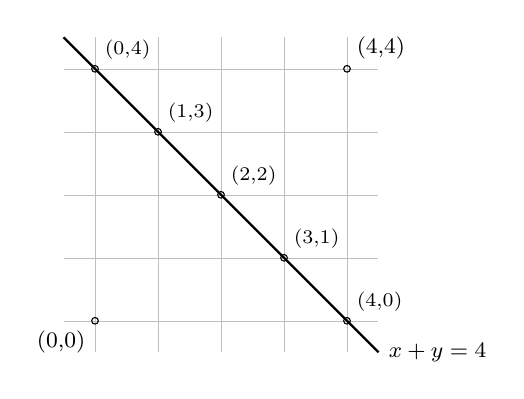
\begin{tikzpicture}[scale=0.8]
      \draw[very thin, color=gray!50] (-.5,-.5) grid (4.5, 4.5);
%       \foreach \x in {0,...,4}
%       \foreach \y in {0,...,4}
%       \fill (\x,\y) circle (1.5pt);
      \draw (0,0) circle (1.5pt) node[below left] {\footnotesize (0,0)} (4,4) circle (1.5pt) node[above right] {\footnotesize (4,4)};
      \draw[thick] (-.5, 4.5) -- (4.5, -.5) node[right]{\footnotesize $x + y = 4$};
      \draw (0,4) circle (1.5pt) node[above right]{\scriptsize (0,4)} (1,3) circle (1.5pt) node[above right]{\scriptsize (1,3)} (2,2) circle (1.5pt) node[above right]{\scriptsize (2,2)} (3,1) circle (1.5pt) node[above right]{\scriptsize (3,1)} (4,0) circle (1.5pt) node[above right]{\scriptsize (4,0)};
    \end{tikzpicture}
   \end{center}

     How many paths pass through $(0,n)$?  To get to that point, you must travel $n$ units, and $0$ of them are to the right, so there are ${n \choose 0}$ ways to get to $(0,n)$.  From $(0,n)$ to $(n,n)$ takes $n$ steps, and $0$ of them are up.  So there are ${n \choose 0}$ ways to get from $(0,n)$ to $(n,n)$.  Therefore there are ${n \choose 0}{n \choose 0}$ paths from $(0,0)$ to $(n,n)$ through the point $(0,n)$.

     What about through $(1,n-1)$.  There are ${n \choose 1}$ paths to get there ($n$ steps, 1 to the right) and ${n \choose 1}$ paths to complete the journey to $(n,n)$ ($n$ steps, $1$ up).  So there are ${n \choose 1}{n \choose 1}$ paths from $(0,0)$ to $(n,n)$ through $(1,n-1)$.

     In general, to get to $(n,n)$ through the point $(k,n-k)$ we have ${n \choose k}$ paths to the midpoint and then ${n \choose k}$ paths from the midpoint to $(n,n)$.  So there are ${n \choose k}{n \choose k}$ paths from $(0,0)$ to $(n,n)$ through $(k, n-k)$.

     All together then the total paths from $(0,0)$ to $(n,n)$ passing through exactly one of these midpoints is
     \[{n \choose 0}^2 + {n \choose 1}^2 + {n \choose 2}^2 + \cdots + {n \choose n}^2.\]
   \end{proof}
  \end{solution}
\end{example}



\end{document}

	\withanswers\documentclass[12pt]{article}

\usepackage{discrete}

\def\thetitle{Combinatorial Proofs} % will be put in the center header on the first page only.
\def\lefthead{Math 228 Notes} % will be put in the left header
\def\righthead{\thetitle} % will be put in the right header





\begin{document}
\newpage
\section{Combinatorial Proofs}\label{sec:comb-proofs}

\begin{activity}
\begin{questions}
\question The Stanley Cup is decided in a best of 7 tournament between two teams.  In how many ways can your team win?  Let's answer this question two ways:
\begin{parts}
  \part How many of the 7 games does your team need to win?  How many ways can this happen?
  \part What if the tournament goes all 7 games?  So you win the last game.  How many ways can the first 6 games go down?
  \part What if the tournament goes just 6 games?  How many ways can this happen?  What about 5 games?  4 games?
  \part What are the two different ways to compute the number of ways your team can win?  Write down an equation involving binary coefficients (that is, ${n \choose k}$'s).  What pattern in Pascal's triangle is this an example of?
\end{parts}
\question Generalize.  What if the rules changed and you played a best of $9$ tournament (5 wins required)?  What if you played an $n$ game tournament with $k$ wins required to be named champion?
\end{questions}

\end{activity}



\subsection{Patterns in Pascal's Triangle}\label{subsec:patternsPascal}

Have a look again at Pascal's triangle.  Forget for a moment where it comes from - just look at it as a mathematical object.  What do you notice?

\begin{center}
\noindent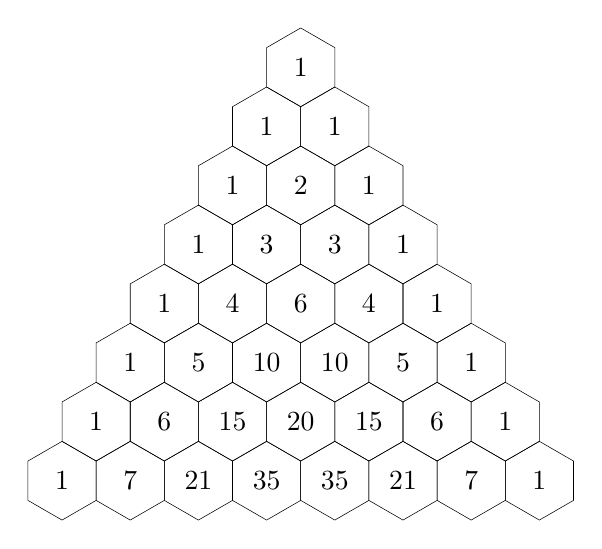
\begin{tikzpicture}
\def\r{.5}
\newcommand{\hexbox}[3]{
  \def\x{-cos{30}*\r*#1+cos{30}*#2*\r*2}
  \def\y{-\r*#1-sin{30}*\r*#1}
  \draw[very thin] (\x,\y) +(90:\r) -- +(30:\r) -- +(-30:\r) -- +(-90:\r) -- +(-150:\r) -- +(150:\r) -- cycle;
  \draw (\x,\y) node{ #3};
}


% Pascal's triangle
%put row of 1's down left side:
  \foreach \row in {0,...,7} {
    \hexbox{\row}{0}{ 1}
  }
%fill in the rest of the triangle:
  \foreach \row in {1,...,7} {
    \pgfmathsetmacro{\entry}{1};
    \foreach \col in {1,...,\row} {
      % iterative formula : val = precval * (row-col+1)/col
      % (+ 0.5 to bypass rounding errors)
     \pgfmathtruncatemacro{\entry}{\entry*((\row-\col+1)/\col)+0.5};
      \global\let\entry=\entry
      \ifnum \entry<100
	\hexbox{\row}{\col}{\entry}
      \else \ifnum \entry<1000
	\hexbox{\row}{\col}{\footnotesize \entry}
      \else \ifnum \entry<10000
	\hexbox{\row}{\col}{\footnotesize \entry}
	\else
	\hexbox{\row}{\col}{\scriptsize \entry}
	\fi
      \fi
      \fi
    }
  }
\end{tikzpicture}

\end{center}

There are lots of patterns hidden away in the triangle, enough to fill a reasonably sized book.  Here are just a few of the most obvious ones:
\begin{enumerate}
  \item The entries on the border of the triangle are all 1.
  \item Any entry not on the border is the sum of the two entries above it.
  \item The triangle is symmetric.  On any row, entries on the left side are mirrored on the right side.
  \item The sum of all entries on a given row is a power of 2. (You should check this!)
\end{enumerate}

We would like to state these observations in a more precise way, and then prove that they are correct.  Now each entry in Pascal's triangle is in fact a binomial coefficient.  The 1 on the very top of the triangle is ${0 \choose 0}$.  The next row (which we will call row 1, even though it is not the top-most row) consists of ${1 \choose 0}$ and ${1 \choose 1}$.  Row 4 (the row 1, 4, 6, 4, 1) consists of the binomial coefficients
\[{4 \choose 0} ~~ {4 \choose 1} ~~ {4 \choose 2} ~~ {4 \choose 3} ~~ {4 \choose 4}.\]
Given this description of the elements in Pascal's triangle, we can rewrite the above observations as follows:
\begin{enumerate}
  \item ${n \choose 0} = 1$ and ${n \choose n} = 1$.
  \item ${n \choose k} = {n-1 \choose k-1} + {n-1 \choose k}$.
  \item ${n \choose k} = {n \choose n-k}$.
  \item ${n\choose 0} + {n \choose 1} + {n \choose 2} + \cdots + {n \choose n} = 2^n$.
\end{enumerate}

Each of these are an example of a {\em binomial identity}\index{binomial identity}: an identity (i.e., equation) involving binomial coefficients.

Our goal is to establish these identities.  We wish to prove that they hold for all values of $n$ and $k$.  These proofs can be done in many ways.  One option would be to give algebraic proofs, using the formula for ${n \choose k}$:
\[{n \choose k} = \frac{n!}{(n-k)!\,k!}.\]
Here's how you might do that for the second identity above.

\begin{example}
  Give an algebraic proof for the binomial identity
  \[{n \choose k} = {n-1\choose k-1} + {n-1 \choose k}.\]
  \begin{proof}
    By the definition of ${n \choose k}$, we have
    \[{n-1 \choose k-1} = \frac{(n-1)!}{(n-1-(k-1))!(k-1)!} = \frac{(n-1)!}{(n-k)!(k-1)!} \hfill \mbox{ and } {n-1 \choose k} = \frac{(n-1)!}{(n-1-k)!k!}.\]
    Thus, starting with the right hand side of the equation we are trying to establish:
    \begin{align*}
      {n-1 \choose k-1} + {n-1 \choose k} & = \frac{(n-1)!}{(n-k)!(k-1)!}+ \frac{(n-1)!}{(n-1-k)!\,k!}\\
      & = \frac{(n-1)!k}{(n-k)!\,k!} + \frac{(n-1)!(n-k)}{(n-k)!\,k!}\\
      & = \frac{(n-1)!(k+n-k)}{(n-k)!\,k!} \\
      & = \frac{n!}{(n-k)!\, k!} \\
      & = {n \choose k}.
    \end{align*}
    The second line (where the common denominator is found) works because $k(k-1)! = k!$ and $(n-k)(n-k-1)! = (n-k)!$.
  \end{proof}

\end{example}

This is certainly a valid proof, but also is entirely useless.  Even if you understand the proof perfectly, it does not tell you {\em why} the identity is true.  A better approach would be to explain what ${n \choose k}$ {\em means} and then say why that is also what ${n-1 \choose k-1} + {n-1 \choose k}$ means.  Let's see how this works for the four identities we observed above.

\begin{example}
  Explain why ${n \choose 0} = 1$ and ${n \choose n} = 1$.
  \begin{solution}
    What do these binomial coefficients tell us? Well, ${n \choose 0}$ gives the number of ways to select 0 objects from a collection of $n$ objects.  There is only one way to do this, namely to not select any of the objects.  Thus ${n \choose 0} = 1$.  Similarly, ${n \choose n}$ gives the number of ways to select $n$ objects from a collection of $n$ objects.  There is only one way to do this: select all $n$ objects.  Thus ${n \choose n} = 1$.

    Alternatively, we know that ${n \choose 0}$ is the number of $n$-bit strings with weight 0.  There is only one such string, the string of all 0's.  So ${n \choose 0} = 1$.  Similarly ${n \choose n}$ is the number of $n$-bit strings with weight $n$.  There is only one string with this property, the string of all 1's.

    Another way: ${n \choose 0}$ gives the number of subsets of a set of size $n$ containing 0 elements.  There is only one such subset, the empty set.  ${n \choose n}$ gives the number of subsets containing $n$ elements.  The only such subset is the original set (of all elements).
  \end{solution}

\end{example}

\begin{example}
  Explain why ${n \choose k} = {n-1 \choose k-1} + {n-1 \choose k}$.
  \begin{solution}
    The easiest way to see this is to consider bit strings.  ${n \choose k}$ is the number of bit strings of length $n$ containing $k$ 1's.  Of all of these strings, some start with a 1 and the rest start with a 0.  First consider all the bit strings which start with a 1.  After the 1, there must be $n-1$ more bits (to get the total length up to $n$) and exactly $k-1$ of them must be 1's (as we already have one, and we need $k$ total).  How many strings are there like that?  There are exactly ${n-1 \choose k-1}$ such bit strings, so of all the length $n$ bit strings containing $k$ 1's, ${n-1 \choose k-1}$ of them start with a 1.  Similarly, there are ${n-1\choose k}$ which start with a 0 (we still need $n-1$ bits and now $k$ of them must be 1's).  Since there are ${n-1 \choose k}$ bit strings containing $n-1$ bits with $k$ 1's, that is the number of length $n$ bit strings with $k$ 1's which start with a 0.

    Another way: consider the question, how many ways can you select $k$ pizza toppings from a menu containing $n$ choices?  One way to do this is just ${n \choose k}$.  Another way to answer the same question is to first decide whether or not you want anchovies.  If you do want anchovies, you still need to pick $k-1$ toppings, now from just $n-1$ choices.  That can be done in ${n-1 \choose k-1}$ ways.  If you do not want anchovies, then you still need to select $k$ toppings from $n-1$ choices (the anchovies are out).  You can do that in ${n-1 \choose k}$ ways.  Since the choices with anchovies are disjoint from the choices without anchovies, the total choices are ${n-1 \choose k-1}+{n-1 \choose k}$.  But wait.  We answered the same question in two different ways, so the two answers must be the same.  Thus ${n \choose k} = {n-1\choose k-1} + {n-1 \choose k}$.

    You can also explain (prove) this identity by counting subsets, or even lattice paths.
  \end{solution}

\end{example}


\begin{example}
  Prove the binomial identity ${n \choose k} = {n \choose n-k}$.
  \begin{solution}
    Why is this true?  ${n \choose k}$ counts the number of ways to select $k$ things from $n$ choices.  On the other hand, ${n \choose n-k}$ counts the number of ways to select $n-k$ things from $n$ choices.  Are these really the same?  Well, what if instead of selecting the $n-k$ things you choose to exclude them.  How many ways are there to choose $n-k$ things to exclude from $n$ choices.  Clearly this is ${n \choose n-k}$ as well (it doesn't matter whether you include or exclude the things once you have chosen them).  And if you exclude $n-k$ things, then you are including the other $k$ things.  So the set of outcomes should be the same.

    Let's try the pizza counting example like we did above.  How many ways are there to pick $k$ toppings from a list of $n$ choices?  On the one hand, the answer is simply ${n \choose k}$.  Alternatively, you could make a list of all the toppings you don't want.  To end up with a pizza containing exactly $k$ toppings, you need to pick $n-k$ toppings to not put on the pizza.  You have ${n \choose n-k}$ choices for the toppings you don't want. Both of these ways give you a pizza with $k$ toppings, in fact all the ways to get a pizza with $k$ toppings.  Thus  these two answers must be the same: ${n \choose k} = {n \choose n-k}$.

    You can also prove (explain) this identity using bit strings, subsets, or lattice paths.  The bit string argument is nice: ${n \choose k}$ counts the number of bit strings of length $n$ with $k$ 1's.  This is also the number of bit string of length $n$ with $k$ 0's (just replace each 1 with a 0 and each 0 with a 1).  But if a string of length $n$ has $k$ 0's, it must have $n-k$ 1's.  And there are exactly ${n\choose n-k}$ strings of length $n$ with $n-k$ 1's.
  \end{solution}
\end{example}

\begin{example}
  Prove the binomial identity ${n\choose 0} + {n \choose 1} + {n\choose 2} + \cdots + {n \choose n} = 2^n$.
  \begin{solution}
    Let's do a ``pizza proof'' again.  We need to find a question about pizza toppings which has $2^n$ as the answer.  How about this: If a pizza joint offers $n$ toppings, how many pizzas can you build using any number of toppings from no toppings to all toppings, using each topping at most once?

    On one hand, the answer is $2^n$.  For each topping you can say ``yes'' or ``no,'' so you have two choices for each topping.

    On the other hand, divide the possible pizzas into disjoint groups: the pizzas with no toppings, the pizzas with one topping, the pizzas with two toppings, etc.  If we want no toppings, there is only one pizza like that (the empty pizza, if you will) but it would be better to think of that number as ${n \choose 0}$ since we choose 0 of the $n$ toppings.  How many pizzas have 1 topping?  We need to choose 1 of the $n$ toppings, so ${n \choose 1}$.  We have:
    \begin{itemize}
      \item[] Pizzas with 0 toppings: ${n \choose 0}$
      \item[] Pizzas with 1 topping: ${n \choose 1}$
      \item[] Pizzas with 2 toppings: ${n \choose 2}$
      \item[] \qquad $\vdots$
      \item[] Pizzas with $n$ toppings: ${n \choose n}$.
    \end{itemize}
    The total number of possible pizzas will be the sum of these, which is exactly the left hand side of the identity we are trying to prove.

    Again, we could have proved the identity using subsets, bit strings, or lattice paths (although the lattice path argument is a little tricky).
  \end{solution}

\end{example}

Hopefully this gives some idea of how explanatory proofs of binomial identities can go.  It is worth pointing out that sometimes more traditional proofs are also nice.\footnote{Most every binomial identity can be proved using mathematical induction, using the recursive definition for ${n \choose k}$.  We will discuss induction in \Cref{sec:induction}.}  For example, consider the following rather slick proof of the last identity.

Recall the binomial theorem:
\[(x + y)^n = {n \choose 0}x^n + {n \choose 1}x^{n-1}y + {n \choose 2}x^{n-2}y^2 + \cdots + {n \choose n-1}x\cdot y^n + {n \choose n}y^n.\]
Let $x = 1$ and $y = 1$.  We get:
\[(1 + 1)^n = {n \choose 0}1^n + {n \choose 1}1^{n-1}1 + {n \choose 2}1^{n-2}1^2 + \cdots + {n \choose n-1}1\cdot 1^n + {n \choose n}1^n.\]
Of course this simplifies to:
\[(2)^n = {n \choose 0} + {n \choose 1} + {n \choose 2} + \cdots + {n \choose n-1} + {n \choose n}.\]
Something fun to try: Let $x = 1$ and $y = 2$.  Neat huh?

\subsection{More Proofs}\label{subsec:moreProofs}

The explanatory proofs given in the above examples are typically called {\em combinatorial proofs}.  In general, to give a combinatorial proof for a binomial identity, say $A = B$ you do the following:
\begin{enumerate}
  \item Find a counting problem you will be able to answer in two ways.
  \item Explain why one answer to the counting problem is $A$.
  \item Explain why the other answer to the counting problem is $B$.
\end{enumerate}

Since both $A$ and $B$ are the answers to the same question, we must have $A = B$.

The tricky thing is coming up with the question.  This is not always obvious, but it gets easier the more counting problems you solve.  You will start to recognize types of answers as the answers to types of questions.  More often what will happen is you will be solving a counting problem and happen to think up two different ways of finding the answer.  Now you have a binomial identity and the proof is right there.  The proof \emph{is} the problem you just solved together with your two solutions.

For example, consider this counting question:

\begin{quote}
  How many 10-letter words use exactly four A's, three B's, two C's and one D?
\end{quote}

Let's try to solve this problem.  We have 10 spots for letters to go.  Four of those need to be A's.  We can pick the four A-spots in ${10 \choose 4}$ ways.  Now where can we put the B's?  Well there are only 6 spots left, we need to pick $3$ of them.  This can be done in ${6 \choose 3}$ ways.  The two C's need to go in two of the 3 remaining spots, so we have ${3 \choose 2}$ ways of doing that.  That leaves just one spot of the D, but we could write that 1 choice as ${1 \choose 1}$.  Thus the answer is:
\[{10 \choose 4}{6 \choose 3}{3 \choose 2}{1 \choose 1}.\]
But why stop there?  We can find the answer another way too.  First let's decide where to put the one D: we have 10 spots, we need to choose 1 of them, so this can be done in ${10 \choose 1}$ ways.  Next, choose one of the ${9 \choose 2}$ ways to place the two C's.  We now have $7$ spots left, and three of them need to be filled with B's.  There are ${7 \choose 3}$ ways to do this.  Finally the A's can be placed in ${4 \choose 4}$ (that is, only one) ways.  So another answer to the question is
\[{10 \choose 1}{9 \choose 2}{7 \choose 3}{4 \choose 4}.\]
Interesting.  This gives us the binomial identity:
\[{10 \choose 4}{6 \choose 3}{3 \choose 2}{1 \choose 1} = {10 \choose 1}{9 \choose 2}{7 \choose 3}{4 \choose 4}.\]
Here are a couple of other binomial identities with combinatorial proofs.

\begin{example}
  Prove the identity
  \[1 n + 2(n-1) + 3  (n-2) + \cdots + (n-1) 2 + n  1 = {n+2 \choose 3}.\]
  \begin{solution}
    To give a combinatorial proof we need to think up a question we can answer in two ways: one way needs to give the left-hand-side of the identity, the other way needs to be the right-hand-side of the identity.  Our clue to what question to ask comes from the right hand side: ${n+2 \choose 3}$ counts the number of ways to select 3 things from a group of $n+2$ things.  Let's name those things $1, 2, 3, \ldots, n+2$.  In other words, we want to find 3-element subsets of those numbers (since order should not matter, subsets are exactly the right thing to think about).  We will have to be a bit clever to explain why the left-hand-side also gives the number of these subsets.  Here's the proof.

    \begin{proof}
      Consider the question ``How many 3-element subsets are there of the set $\{1,2,3,\ldots, n+2\}$?''  We answer this in two ways:

      \underline{Answer 1}: We must select 3 elements from the collection of $n+2$ elements.  This can be done in ${n+2 \choose 3}$ ways.

      \underline{Answer 2}: Break this problem up into cases by what the middle number in the subset is.  Say each subset is $\{a,b,c\}$ written in increasing order.  We count the number of subsets for each distinct value of $b$.  The smallest possible value of $b$ is $2$, and the largest is $n+1$.

      When $b = 2$, there are $1 \cdot n$ subsets: 1 choice for $a$ and $n$ choices (3 through $n+2$) for $c$.

      When $b = 3$, there are $2 \cdot (n-1)$ subsets: 2 choices for $a$ and $n-1$ choices for $c$.

      When $b = 4$, there are $3 \cdot (n-2)$ subsets: 3 choices for $a$ and $n-2$ choices for $c$.

      And so on.  When $b = n+1$, there are $n$ choices for $a$ and only 1 choice for $c$, so $n \cdot 1$ subsets.

      Therefore the total number of subsets is \[1 n + 2 (n-1) + 3  (n-2) + \cdots + (n-1)2 + n  1.\]

      Since Answer 1 and Answer 2 are answers to the same question, they must be equal.  Therefore
      \[1 n + 2 (n-1) + 3  (n-2) + \cdots + (n-1) 2 + n  1 = {n+2 \choose 3}.\]

    \end{proof}

  \end{solution}

\end{example}


\begin{example}
  Prove the binomial identity
  \[{n \choose 0}^2 + {n \choose 1}^2 + {n \choose 2}^2 + \cdots + {n \choose n}^2 = {2n \choose n}.\]
  \begin{solution}
    We will give two different proofs of this fact.  The first will be very similar to the previous example (counting subsets).  The second proof is a little slicker, using lattice paths.

    \begin{proof}
      Consider the question: ``How many pizzas can you make using $n$ toppings when there are $2n$ toppings to choose from?''

      \underline{Answer 1}:  There are $2n$ toppings, from which you must choose $n$.  This can be done in ${2n \choose n}$ ways.

      \underline{Answer 2}: Divide the toppings into two groups of $n$ toppings (perhaps $n$ meats and $n$ veggies).  Any choice of $n$ toppings must include some number from the first group and some number from the second group.  Consider each possible number of meat toppings separately:

      0 meats: ${n \choose 0}{n \choose n}$, since you need to choose 0 of the $n$ meats and $n$ of the $n$ veggies.

      1 meat: ${n \choose 1}{n \choose n-1}$, since you need 1 of $n$ meats so $n-1$ of $n$ veggies.

      2 meats: ${n \choose 2}{n \choose n-2}$.  Choose 2 meats and the remaining $n-2$ toppings from the $n$ veggies.

      And so on.  The last case is $n$ meats, which can be done in ${n \choose n}{n \choose 0}$ ways.

      Thus the total number of pizzas possible is
      \[{n \choose 0}{n \choose n} + {n \choose 1}{n \choose n-1} + {n \choose 2}{n \choose n-2} + \cdots + {n \choose n}{n \choose 0}.\]
      This is not quite the left hand side \ldots yet.  Notice that ${n \choose n} = {n \choose 0}$ and ${n \choose n-1} = {n  \choose 1}$ and so on, by the symmetry formula.  Thus we do indeed get
      \[{n \choose 0}^2 + {n \choose 1}^2 + {n \choose 2}^2 + \cdots + {n \choose n}^2.\]
    \end{proof}

    Here's the second proof:

    \begin{proof}
      Consider the question: How many lattice paths are there from $(0,0)$ to $(n,n)$?

      \underline{Answer 1}: We must travel $2n$ units, and $n$ of them must be in the up direction.  Thus there are ${2n \choose n}$ paths.

      \underline{Answer 2}: Note that any path from $(0,0)$ to $(n,n)$ must cross the line $x + y = n$.  That is, any path must pass through exactly one of the points: $(0,n)$, $(1,n-1)$, $(2,n-2)$, \ldots, $(n, 0)$.  For example, this is what happens in the case $n = 4$:

    \begin{center}
    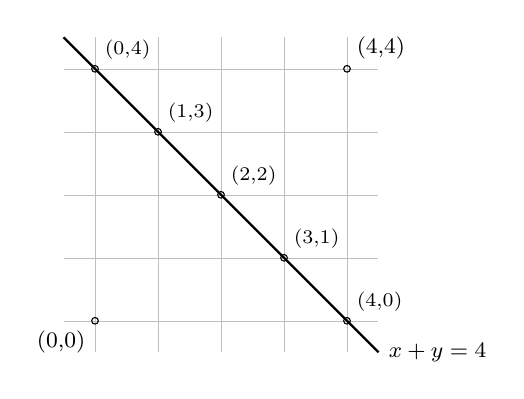
\begin{tikzpicture}[scale=0.8]
      \draw[very thin, color=gray!50] (-.5,-.5) grid (4.5, 4.5);
%       \foreach \x in {0,...,4}
%       \foreach \y in {0,...,4}
%       \fill (\x,\y) circle (1.5pt);
      \draw (0,0) circle (1.5pt) node[below left] {\footnotesize (0,0)} (4,4) circle (1.5pt) node[above right] {\footnotesize (4,4)};
      \draw[thick] (-.5, 4.5) -- (4.5, -.5) node[right]{\footnotesize $x + y = 4$};
      \draw (0,4) circle (1.5pt) node[above right]{\scriptsize (0,4)} (1,3) circle (1.5pt) node[above right]{\scriptsize (1,3)} (2,2) circle (1.5pt) node[above right]{\scriptsize (2,2)} (3,1) circle (1.5pt) node[above right]{\scriptsize (3,1)} (4,0) circle (1.5pt) node[above right]{\scriptsize (4,0)};
    \end{tikzpicture}
   \end{center}

     How many paths pass through $(0,n)$?  To get to that point, you must travel $n$ units, and $0$ of them are to the right, so there are ${n \choose 0}$ ways to get to $(0,n)$.  From $(0,n)$ to $(n,n)$ takes $n$ steps, and $0$ of them are up.  So there are ${n \choose 0}$ ways to get from $(0,n)$ to $(n,n)$.  Therefore there are ${n \choose 0}{n \choose 0}$ paths from $(0,0)$ to $(n,n)$ through the point $(0,n)$.

     What about through $(1,n-1)$.  There are ${n \choose 1}$ paths to get there ($n$ steps, 1 to the right) and ${n \choose 1}$ paths to complete the journey to $(n,n)$ ($n$ steps, $1$ up).  So there are ${n \choose 1}{n \choose 1}$ paths from $(0,0)$ to $(n,n)$ through $(1,n-1)$.

     In general, to get to $(n,n)$ through the point $(k,n-k)$ we have ${n \choose k}$ paths to the midpoint and then ${n \choose k}$ paths from the midpoint to $(n,n)$.  So there are ${n \choose k}{n \choose k}$ paths from $(0,0)$ to $(n,n)$ through $(k, n-k)$.

     All together then the total paths from $(0,0)$ to $(n,n)$ passing through exactly one of these midpoints is
     \[{n \choose 0}^2 + {n \choose 1}^2 + {n \choose 2}^2 + \cdots + {n \choose n}^2.\]
   \end{proof}
  \end{solution}
\end{example}



\end{document}


	\input{chapters/Counting-StarsAndBars}
	\withanswers\input{exercises/Counting-StarsAndBars}

	\documentclass[12pt]{article}

\usepackage{discrete}

\def\thetitle{Advanced Counting} % will be put in the center header on the first page only.
\def\lefthead{Math 228 Notes} % will be put in the left header
\def\righthead{\thetitle} % will be put in the right header




\begin{document}




\section{Advanced Counting Using PIE}\label{sec:advPIE}
\begin{activity}

\begin{questions}
\question You have 11 identical mini key-lime pies to give to 4 children.  However, you don't want any kid to get more than 3 pies.  How many ways can you distribute the pies?
\begin{parts}
\part How many ways are there to distribute the pies without any restriction?

\part Let's get rid of the ways that one or more kid gets too many pies.  How many ways are there to distribute the pies if Al gets too many pies?  What if Bruce gets too many?  Or Cat?  Or Dent?

\part What if two kids get too many pies?  How many ways can this happen?  Does it matter which two kids you pick to overfeed?

\part Is it possible that three kids get too many pies?  If so, how many ways can this happen?

\part How should you combine all the numbers you found above to answer the original question?

\end{parts}
\question Suppose now you have 13 pies and 7 children.  No child can have more than 2 pies.  How many ways can you distribute the pies?



\end{questions}
\end{activity}


Stars and bars allows us to count the number of ways to distribute 10 cookies to 3 kids and natural number solutions to $x+y+z = 11$, for example.  A relatively easy modification allows us to put a \emph{lower bound} restriction on these problems: perhaps each kid must get at least two cookies or $x,y,z \ge 2$.  This was done by first assigning each kid (or variable) 2 cookies (or units) and then distributing the rest using stars and bars.

What if we wanted an \emph{upper bound} restriction?  For example, we might insist that no kid gets more than 4 cookies or that $x, y, z \le 4$.  It turns out this is considerably harder, but still possible.  The idea is to count all the distributions and then remove those that violate the condition.  In other words, we must count the number of ways to distribute 11 cookies to 3 kids in which \emph{one or more} of the kids gets more than 4 cookies.  For any particular kid, this is not a problem; we do this using stars and bars.  But how to combine the number of ways for kid A, or B or C?  We must use the PIE.


The Principle of Inclusion/Exclusion (PIE) gives a method for finding the cardinality of the union of not necessarily disjoint sets.  We saw in \Cref{sec:PIE} how this works with three sets.  To find how many things are in \emph{one or more} of the sets $A$, $B$, and $C$, we should just add up the number of things in each of these sets.  However, if there is any overlap among the sets, those elements are counted multiple times.  So we subtract the things in each intersection of a pair of sets.  But doing this removes elements which are in all three sets once too often, so we need to add it back in.  In terms of cardinality of sets, we have
\[|A \cup B \cup C| = |A| + |B| + |C| - |A \cap B| - |A \cap C| - |B \cap C| + |A\cap B \cap C|.\]

\begin{example}
Three kids, Alberto, Bernadette, and Carlos, decide to share 11 cookies.  They wonder how many ways they could split the cookies up provided that none of them receive more than 4 cookies (someone receiving no cookies is for some reason acceptable to these kids).

\begin{solution}
Without the ``no more than 4'' restriction, the answer would be ${13 \choose 2}$, using 11 stars and 2 bars (separating the three kids).  Now count the number of ways that one or more of the kids violates the condition, i.e., gets at least 4 cookies.

Let $A$ be the set of outcomes in which Alberto gets more than 4 cookies.  Let $B$ be the set of outcomes in which Bernadette gets more than 4 cookies.  Let $C$ be the set of outcomes in which Carlos gets more than 4 cookies.  We then are looking (for the sake of subtraction) for the size of the set $A \cup B \cup C$.  Using PIE, we must find the sizes of $|A|$, $|B|$, $|C|$, $|A\cap B|$ and so on.  Here is what we find.

\begin{itemize}
\item[] $|A| = {8 \choose 2}$.  First give Alberto 5 cookies, then distribute the remaining 6 to the three kids without restrictions, using 6 stars and 2 bars.
\item[] $|B| = {8 \choose 2}$.  Just like above, only now Bernadette gets 5 cookies at the start.
\item[] $|C| = {8 \choose 2}$.  Carlos gets 5 cookies first.

\item[] $|A \cap B| = {3 \choose 2}$.  Give Alberto and Bernadette 5 cookies each, leaving 1 (star) to distribute to the three kids (2 bars).

\item[] $|A \cap C| = {3 \choose 2}$.  Alberto and Carlos get 5 cookies first.

\item[] $|B \cap C| = {3 \choose 2}$.  Bernadette and Carlos get 5 cookies first.

\item[] $|A \cap B \cap C| = 0$.  It is not possible for all three kids to get 4 or more cookies.
\end{itemize}

Combining all of these we see
\[|A \cup B \cup C| = {8 \choose 2} + {8 \choose 2} + {8 \choose 2} - {3 \choose 2} - {3 \choose 2} - {3 \choose 2} + 0 = 75.\]

Thus the answer to the original question is ${13 \choose 2} - 75 = 78 - 75 = 3$.  This makes sense now that we see it.  The only way to ensure that no kid gets more than 4 cookies is to give two kids 4 cookies and one kid 3; there are three choices for which kid that should be.  We could have found the answer much quicker through this observation, but the point of the example is to illustrate that PIE works!
\end{solution}
\end{example}


For four or more sets, we do not write down a formula for PIE.  Instead, we just think of the principle: add up all the elements in single sets, then subtract out things you counted twice (elements in the intersection of a {\em pair} of sets), then add back in elements you removed too often (elements in the intersection of groups of three sets), then take back out elements you added back in too often (elements in the intersection of groups of four sets), then add back in, take back out, add back in, etc.  This would be very difficult if it wasn't for the fact that in these problems, all the cardinalities of the single sets are equal, as are all the cardinalities of the intersections of two sets, and that of three sets, and so on.  Thus we can group all of these together and multiply by how many different combinations of 1, 2, 3,\ldots sets there are.


\begin{example}
How many ways can you distribute 10 cookies to 4 kids so that no kid gets more than 2 cookies?

\begin{solution}
To answer this, we will subtract all the outcomes in which a kid gets 3 or more cookies.  How many outcomes are there like that?  We can force kid A to eat 3 or more cookies by giving him 3 cookies before we start.  Doing so reduces the problem to one in which we have 7 cookies to give to 4 kids without any restrictions.  In that case, we have 7 stars (the 7 remaining cookies) and 3 bars (one less than the number of kids) so we can distribute the cookies in ${10 \choose 3}$ ways.  Of course we could choose any one of the 4 kids to give too many cookies, so it would appear that there are ${4 \choose 1}{10 \choose 3}$ ways to distribute the cookies giving too many to one kid.  But in fact, we have over counted.

We must get rid of the outcomes in which two kids have too many cookies.  There are ${4 \choose 2}$ ways to select 2 kids to give extra cookies.  It takes 6 cookies to do this, leaving only 4 cookies.  So we have 4 stars and still 3 bars.  The remaining 4 cookies can thus be distributed in ${7 \choose 3}$ ways (for each of the ${4 \choose 2}$ choices of which 2 kids to over-feed).

But now we have removed too much.  We must add back in all the ways to give too many cookies to three kids.  This uses 9 cookies, leaving only 1 to distribute to the 4 kids using stars and bars, which can be done in ${4 \choose 3}$ ways.  We must consider this outcome for every possible choice of which three kids we over-feed, and there are ${4 \choose 3}$ ways of selecting that set of 3 kids.

Next we would subtract all the ways to give four kids too many cookies, but in this case, that number is 0.

All together we get that the number of ways to distribute 10 cookies to 4 kids without giving any kid more than 2 cookies is:
\[{13 \choose 3} - \left[{4 \choose 1}{10 \choose 3} - {4 \choose 2}{7 \choose 3} + {4\choose 3}{4\choose 3}\right] = 286 - [480 - 210 + 16] = 0.\]
This makes sense: there is NO way to distribute 10 cookies to 4 kids and make sure that nobody gets more than 2.  It is slightly surprising that \[{13 \choose 3} = \left[{4 \choose 1}{10 \choose 3} - {4 \choose 2}{7 \choose 3} + {4\choose 3}{4\choose 3}\right]\] but since PIE works, this equality must hold.
\end{solution}
\end{example}

Just so you don't think that these problems always have easier solutions, consider the following example.

\begin{example}
Earlier we counted the number of solutions to the equation
\[x_1 + x_2 + x_3 + x_4 + x_5 = 13.\]

How many of those solutions have $0 \le x_i \le 3$ for each $x_i$?


\begin{solution}
 We must subtract off the number of solutions in which one or more of the variables has a value greater than 3.  We will need to use PIE because counting the number of solutions for which each of the five variables separately are greater than 3 counts solutions multiple times.  Here is what we get:
    \begin{itemize}
      \item Total solutions: ${17 \choose 4}$.
      \item Solutions where $x_1 > 3$: ${13 \choose 4}$.  Give $x_1$ 4 units first, then distribute the remaining 9 units to the 5 variables.
      \item Solutions where $x_1 > 3$ and $x_2 > 3$: ${9 \choose 4}$. After you give 4 units to $x_1$ and another 4 to $x_2$, you only have 5 units left to distribute.
      \item Solutions where $x_1 > 3$, $x_2 > 3$ and $x_3 > 3$: ${5 \choose 4}$.
      \item Solutions where $x_1 > 3$, $x_2 > 3$, $x_3 > 3$, and $x_4 > 3$: 0.
    \end{itemize}
    We also need to account for the fact that we could choose any of the five variables in the place of $x_1$ above, any pair of variables in the place of $x_1$ and $x_2$ and so on.  It is because of this that the double counting occurs, so we need to use PIE.  All together we have that the number of solutions with $0 \le x_i \le 3$ is
    \[{17 \choose 4} - \left[{5\choose 1}{13 \choose 4} - {5 \choose 2}{9 \choose 4} + {5 \choose 3}{5 \choose 4}\right] = 15.\]
  \end{solution}
\end{example}




\newpage
\subsection{Counting Derangements}\label{subsec:derangements}

\begin{activity}
For your senior prank, you decide to switch the nameplates on your favorite 5 professors' doors.  So that none of them feel left out, you want to make sure that all of the nameplates end up on the wrong door.  How many ways can this be accomplished?
\end{activity}


The advanced use of PIE has applications beyond stars and bars.  A {\em derangement}\index{derangement} of $n$ elements $\{1,2,3,\ldots, n\}$ is a permutation in which no element is fixed.  For example, there are $6$ permutations of the three elements $\{1,2,3\}$:
\[123 ~~ 132 ~~ 213 ~~ 231 ~~ 312 ~~ 321.\]
but most of these have one or more elements fixed: $123$ has all three elements fixed, $132$ has the first element fixed (1 is in its original first position), and so on.  In fact, the only derangements of three elements are
\[231 \mbox{  and  }312.\]
If we go up to 4 elements, there are 24 permutations (because we have 4 choices for the first element, 3 choices for the second, 2 choices for the third leaving only 1 choice for the last).  How many of these are derangements?  If you list out all 24 permutations and eliminate those which are not derangements, you will be left with just 9 derangements.  Let's see how we can get that number using PIE.

\begin{example}
  How many derangements are there of 4 elements?
  \begin{solution}
    We count all permutations, and subtract those which are not derangements.  There are $4! = 24$ permutations of 4 elements.  Now for a permutation to {\em not} be a derangement, at least one of the 4 elements must be fixed.  There are ${4 \choose 1}$ choices for which single element we fix.  Once fixed, we need to find a permutation of the other three elements. There are $3!$ permutations on 3 elements.  But now we have counted too many non-derangements, so we must subtract those permutations which fix two elements.  There are ${4 \choose 2}$ choices for which two elements we fix, and then for each pair, $2!$ permutations of the remaining elements.  But this subtracts too many, so add back in permutations which fix 3 elements, all ${4 \choose 3}1!$ of them.  Finally subtract the ${4 \choose 4}0!$ permutations (recall $0! = 1$) which fix all four elements.  All together we get that the number of derangements of 4 elements is:
    \[4! - \left[{4 \choose 1}3! - {4 \choose 2}2! + {4 \choose 3} 1! - {4 \choose 4}0!\right] = 24 - 15 = 9.\]

  \end{solution}

\end{example}

Of course we can use a similar formula to count the derangements on any number of elements.  However, the more elements we have, the longer the formula gets.  Here is another example.

\begin{example}
  Five gentlemen attend a party, leaving their hats at the door.  At the end of the party, they hastily grab hats on their way out.  How many different ways could this happen so that none of the gentlemen leave with their own hat?

  \begin{solution}
    We are counting derangements on 5 elements.  There are $5!$ ways for the gentlemen to grab hats in any order - but many of these permutations will result in someone getting their own hat.  So we subtract all the ways in which one or more of the men get their own hat.  In other words, we subtract the non-derangements. Doing so requires PIE.  Thus the answer is:

    \[5! - \left[{5 \choose 1}4! - {5 \choose 2}3! + {5 \choose 3}2! - {5 \choose 4}1! + {5 \choose 5}0!\right].\]
  \end{solution}

\end{example}


%\subsection*{Counting Surjections}
%
%




\end{document}

	\withanswers\documentclass[12pt]{article}

\usepackage{discrete}

\def\thetitle{Advanced Counting} % will be put in the center header on the first page only.
\def\lefthead{Math 228 Notes} % will be put in the left header
\def\righthead{\thetitle} % will be put in the right header




\begin{document}




\section{Advanced Counting Using PIE}\label{sec:advPIE}
\begin{activity}

\begin{questions}
\question You have 11 identical mini key-lime pies to give to 4 children.  However, you don't want any kid to get more than 3 pies.  How many ways can you distribute the pies?
\begin{parts}
\part How many ways are there to distribute the pies without any restriction?

\part Let's get rid of the ways that one or more kid gets too many pies.  How many ways are there to distribute the pies if Al gets too many pies?  What if Bruce gets too many?  Or Cat?  Or Dent?

\part What if two kids get too many pies?  How many ways can this happen?  Does it matter which two kids you pick to overfeed?

\part Is it possible that three kids get too many pies?  If so, how many ways can this happen?

\part How should you combine all the numbers you found above to answer the original question?

\end{parts}
\question Suppose now you have 13 pies and 7 children.  No child can have more than 2 pies.  How many ways can you distribute the pies?



\end{questions}
\end{activity}


Stars and bars allows us to count the number of ways to distribute 10 cookies to 3 kids and natural number solutions to $x+y+z = 11$, for example.  A relatively easy modification allows us to put a \emph{lower bound} restriction on these problems: perhaps each kid must get at least two cookies or $x,y,z \ge 2$.  This was done by first assigning each kid (or variable) 2 cookies (or units) and then distributing the rest using stars and bars.

What if we wanted an \emph{upper bound} restriction?  For example, we might insist that no kid gets more than 4 cookies or that $x, y, z \le 4$.  It turns out this is considerably harder, but still possible.  The idea is to count all the distributions and then remove those that violate the condition.  In other words, we must count the number of ways to distribute 11 cookies to 3 kids in which \emph{one or more} of the kids gets more than 4 cookies.  For any particular kid, this is not a problem; we do this using stars and bars.  But how to combine the number of ways for kid A, or B or C?  We must use the PIE.


The Principle of Inclusion/Exclusion (PIE) gives a method for finding the cardinality of the union of not necessarily disjoint sets.  We saw in \Cref{sec:PIE} how this works with three sets.  To find how many things are in \emph{one or more} of the sets $A$, $B$, and $C$, we should just add up the number of things in each of these sets.  However, if there is any overlap among the sets, those elements are counted multiple times.  So we subtract the things in each intersection of a pair of sets.  But doing this removes elements which are in all three sets once too often, so we need to add it back in.  In terms of cardinality of sets, we have
\[|A \cup B \cup C| = |A| + |B| + |C| - |A \cap B| - |A \cap C| - |B \cap C| + |A\cap B \cap C|.\]

\begin{example}
Three kids, Alberto, Bernadette, and Carlos, decide to share 11 cookies.  They wonder how many ways they could split the cookies up provided that none of them receive more than 4 cookies (someone receiving no cookies is for some reason acceptable to these kids).

\begin{solution}
Without the ``no more than 4'' restriction, the answer would be ${13 \choose 2}$, using 11 stars and 2 bars (separating the three kids).  Now count the number of ways that one or more of the kids violates the condition, i.e., gets at least 4 cookies.

Let $A$ be the set of outcomes in which Alberto gets more than 4 cookies.  Let $B$ be the set of outcomes in which Bernadette gets more than 4 cookies.  Let $C$ be the set of outcomes in which Carlos gets more than 4 cookies.  We then are looking (for the sake of subtraction) for the size of the set $A \cup B \cup C$.  Using PIE, we must find the sizes of $|A|$, $|B|$, $|C|$, $|A\cap B|$ and so on.  Here is what we find.

\begin{itemize}
\item[] $|A| = {8 \choose 2}$.  First give Alberto 5 cookies, then distribute the remaining 6 to the three kids without restrictions, using 6 stars and 2 bars.
\item[] $|B| = {8 \choose 2}$.  Just like above, only now Bernadette gets 5 cookies at the start.
\item[] $|C| = {8 \choose 2}$.  Carlos gets 5 cookies first.

\item[] $|A \cap B| = {3 \choose 2}$.  Give Alberto and Bernadette 5 cookies each, leaving 1 (star) to distribute to the three kids (2 bars).

\item[] $|A \cap C| = {3 \choose 2}$.  Alberto and Carlos get 5 cookies first.

\item[] $|B \cap C| = {3 \choose 2}$.  Bernadette and Carlos get 5 cookies first.

\item[] $|A \cap B \cap C| = 0$.  It is not possible for all three kids to get 4 or more cookies.
\end{itemize}

Combining all of these we see
\[|A \cup B \cup C| = {8 \choose 2} + {8 \choose 2} + {8 \choose 2} - {3 \choose 2} - {3 \choose 2} - {3 \choose 2} + 0 = 75.\]

Thus the answer to the original question is ${13 \choose 2} - 75 = 78 - 75 = 3$.  This makes sense now that we see it.  The only way to ensure that no kid gets more than 4 cookies is to give two kids 4 cookies and one kid 3; there are three choices for which kid that should be.  We could have found the answer much quicker through this observation, but the point of the example is to illustrate that PIE works!
\end{solution}
\end{example}


For four or more sets, we do not write down a formula for PIE.  Instead, we just think of the principle: add up all the elements in single sets, then subtract out things you counted twice (elements in the intersection of a {\em pair} of sets), then add back in elements you removed too often (elements in the intersection of groups of three sets), then take back out elements you added back in too often (elements in the intersection of groups of four sets), then add back in, take back out, add back in, etc.  This would be very difficult if it wasn't for the fact that in these problems, all the cardinalities of the single sets are equal, as are all the cardinalities of the intersections of two sets, and that of three sets, and so on.  Thus we can group all of these together and multiply by how many different combinations of 1, 2, 3,\ldots sets there are.


\begin{example}
How many ways can you distribute 10 cookies to 4 kids so that no kid gets more than 2 cookies?

\begin{solution}
To answer this, we will subtract all the outcomes in which a kid gets 3 or more cookies.  How many outcomes are there like that?  We can force kid A to eat 3 or more cookies by giving him 3 cookies before we start.  Doing so reduces the problem to one in which we have 7 cookies to give to 4 kids without any restrictions.  In that case, we have 7 stars (the 7 remaining cookies) and 3 bars (one less than the number of kids) so we can distribute the cookies in ${10 \choose 3}$ ways.  Of course we could choose any one of the 4 kids to give too many cookies, so it would appear that there are ${4 \choose 1}{10 \choose 3}$ ways to distribute the cookies giving too many to one kid.  But in fact, we have over counted.

We must get rid of the outcomes in which two kids have too many cookies.  There are ${4 \choose 2}$ ways to select 2 kids to give extra cookies.  It takes 6 cookies to do this, leaving only 4 cookies.  So we have 4 stars and still 3 bars.  The remaining 4 cookies can thus be distributed in ${7 \choose 3}$ ways (for each of the ${4 \choose 2}$ choices of which 2 kids to over-feed).

But now we have removed too much.  We must add back in all the ways to give too many cookies to three kids.  This uses 9 cookies, leaving only 1 to distribute to the 4 kids using stars and bars, which can be done in ${4 \choose 3}$ ways.  We must consider this outcome for every possible choice of which three kids we over-feed, and there are ${4 \choose 3}$ ways of selecting that set of 3 kids.

Next we would subtract all the ways to give four kids too many cookies, but in this case, that number is 0.

All together we get that the number of ways to distribute 10 cookies to 4 kids without giving any kid more than 2 cookies is:
\[{13 \choose 3} - \left[{4 \choose 1}{10 \choose 3} - {4 \choose 2}{7 \choose 3} + {4\choose 3}{4\choose 3}\right] = 286 - [480 - 210 + 16] = 0.\]
This makes sense: there is NO way to distribute 10 cookies to 4 kids and make sure that nobody gets more than 2.  It is slightly surprising that \[{13 \choose 3} = \left[{4 \choose 1}{10 \choose 3} - {4 \choose 2}{7 \choose 3} + {4\choose 3}{4\choose 3}\right]\] but since PIE works, this equality must hold.
\end{solution}
\end{example}

Just so you don't think that these problems always have easier solutions, consider the following example.

\begin{example}
Earlier we counted the number of solutions to the equation
\[x_1 + x_2 + x_3 + x_4 + x_5 = 13.\]

How many of those solutions have $0 \le x_i \le 3$ for each $x_i$?


\begin{solution}
 We must subtract off the number of solutions in which one or more of the variables has a value greater than 3.  We will need to use PIE because counting the number of solutions for which each of the five variables separately are greater than 3 counts solutions multiple times.  Here is what we get:
    \begin{itemize}
      \item Total solutions: ${17 \choose 4}$.
      \item Solutions where $x_1 > 3$: ${13 \choose 4}$.  Give $x_1$ 4 units first, then distribute the remaining 9 units to the 5 variables.
      \item Solutions where $x_1 > 3$ and $x_2 > 3$: ${9 \choose 4}$. After you give 4 units to $x_1$ and another 4 to $x_2$, you only have 5 units left to distribute.
      \item Solutions where $x_1 > 3$, $x_2 > 3$ and $x_3 > 3$: ${5 \choose 4}$.
      \item Solutions where $x_1 > 3$, $x_2 > 3$, $x_3 > 3$, and $x_4 > 3$: 0.
    \end{itemize}
    We also need to account for the fact that we could choose any of the five variables in the place of $x_1$ above, any pair of variables in the place of $x_1$ and $x_2$ and so on.  It is because of this that the double counting occurs, so we need to use PIE.  All together we have that the number of solutions with $0 \le x_i \le 3$ is
    \[{17 \choose 4} - \left[{5\choose 1}{13 \choose 4} - {5 \choose 2}{9 \choose 4} + {5 \choose 3}{5 \choose 4}\right] = 15.\]
  \end{solution}
\end{example}




\newpage
\subsection{Counting Derangements}\label{subsec:derangements}

\begin{activity}
For your senior prank, you decide to switch the nameplates on your favorite 5 professors' doors.  So that none of them feel left out, you want to make sure that all of the nameplates end up on the wrong door.  How many ways can this be accomplished?
\end{activity}


The advanced use of PIE has applications beyond stars and bars.  A {\em derangement}\index{derangement} of $n$ elements $\{1,2,3,\ldots, n\}$ is a permutation in which no element is fixed.  For example, there are $6$ permutations of the three elements $\{1,2,3\}$:
\[123 ~~ 132 ~~ 213 ~~ 231 ~~ 312 ~~ 321.\]
but most of these have one or more elements fixed: $123$ has all three elements fixed, $132$ has the first element fixed (1 is in its original first position), and so on.  In fact, the only derangements of three elements are
\[231 \mbox{  and  }312.\]
If we go up to 4 elements, there are 24 permutations (because we have 4 choices for the first element, 3 choices for the second, 2 choices for the third leaving only 1 choice for the last).  How many of these are derangements?  If you list out all 24 permutations and eliminate those which are not derangements, you will be left with just 9 derangements.  Let's see how we can get that number using PIE.

\begin{example}
  How many derangements are there of 4 elements?
  \begin{solution}
    We count all permutations, and subtract those which are not derangements.  There are $4! = 24$ permutations of 4 elements.  Now for a permutation to {\em not} be a derangement, at least one of the 4 elements must be fixed.  There are ${4 \choose 1}$ choices for which single element we fix.  Once fixed, we need to find a permutation of the other three elements. There are $3!$ permutations on 3 elements.  But now we have counted too many non-derangements, so we must subtract those permutations which fix two elements.  There are ${4 \choose 2}$ choices for which two elements we fix, and then for each pair, $2!$ permutations of the remaining elements.  But this subtracts too many, so add back in permutations which fix 3 elements, all ${4 \choose 3}1!$ of them.  Finally subtract the ${4 \choose 4}0!$ permutations (recall $0! = 1$) which fix all four elements.  All together we get that the number of derangements of 4 elements is:
    \[4! - \left[{4 \choose 1}3! - {4 \choose 2}2! + {4 \choose 3} 1! - {4 \choose 4}0!\right] = 24 - 15 = 9.\]

  \end{solution}

\end{example}

Of course we can use a similar formula to count the derangements on any number of elements.  However, the more elements we have, the longer the formula gets.  Here is another example.

\begin{example}
  Five gentlemen attend a party, leaving their hats at the door.  At the end of the party, they hastily grab hats on their way out.  How many different ways could this happen so that none of the gentlemen leave with their own hat?

  \begin{solution}
    We are counting derangements on 5 elements.  There are $5!$ ways for the gentlemen to grab hats in any order - but many of these permutations will result in someone getting their own hat.  So we subtract all the ways in which one or more of the men get their own hat.  In other words, we subtract the non-derangements. Doing so requires PIE.  Thus the answer is:

    \[5! - \left[{5 \choose 1}4! - {5 \choose 2}3! + {5 \choose 3}2! - {5 \choose 4}1! + {5 \choose 5}0!\right].\]
  \end{solution}

\end{example}


%\subsection*{Counting Surjections}
%
%




\end{document}


	\input{chapters/Counting-Functions}
	\withanswers\input{exercises/Counting-Functions}

	\input{chapters/Counting-Conclusion}
	\withanswers\input{exercises/Counting-Conclusion}
	\noanswers\starthwsol\input{homework/Counting}\finishhwsol


\chapter[Sequences]{Sequences}

	\input{chapters/Sequences-Intro}
	\withanswers\input{exercises/Sequences-Intro}

	\input{chapters/Sequences-ArithmeticGeometric}
	\withanswers\input{exercises/Sequences-ArithmeticGeometric}

	\input{chapters/Sequences-PolynomialFitting}
	\withanswers\input{exercises/Sequences-PolynomialFitting}

	\documentclass[12pt]{article}

\usepackage{discrete}

\def\thetitle{Sequences} % will be put in the center header on the first page only.
\def\lefthead{Math 228 Notes} % will be put in the left header
\def\righthead{\thetitle} % will be put in the right header

\begin{document}
\section{Solving Recurrence Relations}\label{sec:recurrence}

\begin{activity}
Consider the recurrence relation
\[a_n = 5a_{n-1} - 6a_{n-2}.\]

\begin{questions}
\question What sequence do you get if the initial conditions are $a_0 = 1$, $a_1 = 2$?  Give a closed formula for this sequence.
\question What sequence do you get if the initial conditions are $a_0 = 1$, $a_1 = 3$?  Give a closed formula.
\question What if $a_0 = 2$ and $a_1 = 5$?  Find a closed formula.
\end{questions}
\end{activity}

We have seen that it is often easier to find recursive definitions than closed formulas.  Lucky for us, there are a few techniques for converting recursive definitions to closed formulas.  Doing so is called \emph{solving a recurrence relation}.  Recall that the recurrence relation is a recursive definition without the initial conditions.  For example, the recurrence relation for the Fibonacci sequence\index{Fibonacci sequence} is $\gls{Fn} = F_{n-1} + F_{n-2}$.  (This, together with the initial conditions $F_0 = 0$ and $F_1 = 1$ give the entire recursive definition for the sequence.)

\begin{example}
  Find a recurrence relation and initial conditions for $1, 5, 17, 53, 161, 485\ldots$.
  \begin{solution}
    Finding the recurrence relation would be easier if we had some context for the problem (like the Tower of Hanoi, for example).  Alas, we have only the sequence.  Remember, the recurrence relation tells you how to get from previous terms to future terms.  What is going on here?  We could look at the differences between terms: $4, 12, 36, 108, \ldots$.  Notice that these are growing by a factor of 3.  Is the original sequence as well?  $1\cdot 3 = 3$, $5 \cdot 3 = 15$, $17 \cdot 3 = 51$ and so on.  It appears that we always end up with 2 less than the next term.  Aha!

    So $a_n = 3a_{n-1} + 2$ is our recurrence relation and the initial condition is $a_0 = 1$.
  \end{solution}

\end{example}


We are going to try to {\em solve} these recurrence relations.  By this we mean something very similar to solving differential equations: we want to find a function of $n$ (a closed formula) which satisfies the recurrence relation, as well as the initial condition.\footnote{Recurrence relations are sometimes called difference equations since they can describe the difference between terms and this highlights the relation to differential equations further.} Just like for differential equations, finding a solution might be tricky, but checking that the solution is correct is easy.

 \begin{example}
    Check that $a_n = 2^n + 1$ is a solution to the recurrence relation $a_n = 2a_{n-1} - 1$ with $a_1 = 3$.
    \begin{solution}
      First, it is easy to check the initial condition: $a_1$ should be $2^1 + 1$ according to our closed formula.  But $2^1 + 1 = 3$, which is what we want.  To check that our proposed solution satisfies the recurrence relation, try plugging it in.
      \[2a_{n-1} - 1 = 2(2^{n-1} + 1) - 1 = 2^n + 2 - 1 = 2^n +1 = a_n.\]
      That's what our recurrence relation says!  We have a solution.
    \end{solution}

 \end{example}


%We will consider three techniques for solving recurrence relations: Telescoping, Iteration and the Characteristic Root Technique.

Sometimes we can be clever and solve a recurrence relation by inspection.  We generate the sequence using the recurrence relation and keep track of what we are doing so that we can see how to jump to finding just the $a_n$ term.  Here are two examples of how you might do that.
%
%\subsection{Telescoping}

{\em Telescoping}\index{telescoping} refers to the phenomenon when many terms in a large sum cancel out - so the sum ``telescopes.''  For example:
\[(2 - 1) + (3 - 2) + (4 - 3) + \cdots + (100 - 99) + (101 - 100) = -1 + 101\]
because every third term looks like: $2 + -2 = 0$, and then $3 + -3 = 0$ and so on.

We can use this behavior to solve recurrence relations.  Here is an example.

\begin{example}
  Solve the recurrence relation $a_n = a_{n-1} + n$ with initial term $a_0 = 4$.

  \begin{solution}
    To get a feel for the recurrence relation, write out the first few terms of the sequence: $4, 5, 7, 10, 14, 19, \ldots$.  Look at the difference between terms.  $a_1 - a_0 = 1$ and $a_2 - a_1 = 2$ and so on.  The key thing here is that the difference between terms is $n$.  We can write this explicitly: $a_n - a_{n-1} = n$.  Of course, we could have arrived at this conclusion directly from the recurrence relation by subtracting $a_{n-1}$ from both sides.

    Now use this equation over and over again, changing $n$ each time:

    \begin{align*}
      a_1 - a_0 &= 1\\
      a_2 - a_1 &= 2\\
      a_3 - a_2 & = 3\\
      \vdots \quad & \quad \vdots \\
      a_n - a_{n-1} & = n.
    \end{align*}
  Add all these equations together.  On the right hand side, we get the sum $1 + 2 + 3 + \cdots + n$.  We already know this can be simplified to $\frac{n(n+1)}{2}$.  What happens on the left hand side?  We get
  \[(a_1 - a_0) + (a_2 - a_1) + (a_3 - a_2) + \cdots (a_{n-1} - a_{n-2})+ (a_n - a_{n-1}).\]
  This sum telescopes.  We are left with only the $-a_0$ from the first equation and the $a_n$ from the last equation.  Putting this all together we have $-a_0 + a_n = \frac{n(n+1)}{2}$ or $a_n = \frac{n(n+1)}{2} + a_0$.  But we know that $a_0 = 4$.  So the solution to the recurrence relation, subject to the initial condition is
  \[a_n = \frac{n(n+1)}{2} + 4.\]
  (Now that we know that, we should notice that the sequence is the result of adding 4 to each of the triangular numbers.)
  \end{solution}

\end{example}

The above example shows a way to solve recurrence relations of the form $a_n = a_{n-1} + f(n)$ where $\sum_{k = 1}^n f(k)$ has a known closed formula.  If you rewrite the recurrence relation as $a_n - a_{n-1} = f(n)$, and then add up all the different equations with $n$ ranging between 1 and $n$, the left hand side will always give you $a_n - a_0$.  The right hand side will be $\sum_{k = 1}^n f(k)$, which is why we need to know the closed formula for that sum.

However, telescoping will not help us with a recursion such as $a_n = 3a_{n-1} + 2$ since the left hand side will not telescope.  You will have $-3a_{n-1}$'s but only one $a_{n-1}$.  However, we can still be clever if we use {\em iteration}.
%We need another method for this.
%
%\subsection{Iteration}

We have already seen an example of iteration when we found the closed formula for arithmetic and geometric sequences.  The idea is, we {\em iterate}\index{iteration} the process of finding the next term, starting with the known initial condition, up until we have $a_n$.  Then we simplify.  In the arithmetic sequence example, we simplified by multiplying $d$ by the number of times we add it to $a$ when we get to $a_n$, to get from $a_n = a + d + d + d + \cdots + d$ to $a_n = a + dn$.

To see how this works, let's go through the same example we used for telescoping, but this time use iteration.



\begin{example}
  Use iteration to solve the recurrence relation $a_n = a_{n-1} + n$ with $a_0 = 4$.

  \begin{solution}
    Again, start by writing down the recurrence relation when $n = 1$.  This time, don't subtract the $a_{n-1}$ terms to the other side:
    \[a_1 = a_0 + 1.\]
    Now $a_2 = a_1 + 2$, but we know what $a_1$ is.  By substitution, we get
    \[a_2 = (a_0 + 1) + 2.\]
    Now go to $a_3 = a_2 + 3$, using our known value of $a_2$:
    \[a_3 = ((a_0 + 1) + 2) + 3.\]
    We notice a pattern.  Each time, we take the previous term and add the current index.  So
    \[a_n = ((((a_0 + 1) +2)+3)+\cdots + n-1) + n.\]
    Regrouping terms, we notice that $a_n$ is just $a_0$ plus the sum of the integers from $1$ to $n$.  So, since $a_0 = 4$,
    \[a_n = 4 + \frac{n(n+1)}{2}.\]
  \end{solution}

\end{example}

 Of course in this case we still needed to know formula for the sum of $1,\ldots,n$.  Let's try iteration with a sequence for which telescoping doesn't work.

 \begin{example}
   Solve the recurrence relation $a_n = 3a_{n-1} + 2$ subject to $a_0 = 1$.
   \begin{solution}
     Again, we iterate the recurrence relation, building up to the index $n$.
     \begin{align*}
      a_1 &= 3a_0 + 2\\
      a_2 &= 3(a_1) + 2 = 3(3a_0 + 2) + 2\\
      a_3 &= 3[a_2] + 2 = 3[3(3a_0 + 2) + 2] + 2\\
      \vdots & \qquad \vdots \qquad \qquad \vdots \\
      a_n &= 3(a_{n-1}) + 2 = 3(3(3(3\cdots(3a_0 + 2) + 2) + 2)\cdots + 2)+ 2.
     \end{align*}
	 It is difficult to see what is happening here because we have to distribute all those 3's.  Let' try again, this time simplifying a bit as we go.
	      \begin{align*}
      a_1 &= 3a_0 + 2\\
      a_2 &= 3(a_1) + 2 = 3(3a_0 + 2) + 2 = 3^2a_0 + 2\cdot 3 + 2\\
      a_3 &= 3[a_2] + 2 = 3[3^2a_0 + 2\cdot 3 + 2] + 2 = 3^3 a_0 + 2 \cdot 3^2 + 2 \cdot 3 + 2\\
      \vdots & \qquad\quad \vdots \hspace{2in} \vdots \\
      a_n &= 3(a_{n-1}) + 2 = 3(3^{n-1}a_0 + 2 \cdot 3^{n-2} + \cdots +2)+ 2\\
      & \qquad \qquad = 3^n a_0 + 2\cdot 3^{n-1} + 2 \cdot 3^{n-2} + \cdots + 2\cdot 3 + 2.
     \end{align*}
    Now we simplify.  $a_0 = 1$, so we have $3^n + (\cdots)$.  Note that all the other terms have a 2 in them.  In fact, we have a geometric sum with first term $2$ and common ratio $3$.  We have seen how to simplify $2 + 2\cdot 3 + 2 \cdot 3^2 + \cdots + 2\cdot 3^{n-1}$.  We get $\frac{2-2\cdot 3^n}{-2}$ which simplifies to $3^n - 1$.  Putting this together with the first $3^n$ term gives our closed formula:
    \[a_n = 2\cdot 3^n - 1.\]
   \end{solution}
 \end{example}


 Iteration can be messy, but when the recurrence relation only refers to one previous term (and maybe some function of $n$) it can work well.  However, trying to iterate a recurrence relation such as $a_n = 2 a_{n-1} + 3 a_{n-2}$ will be way too complicated.  We would need to keep track of two sets of previous terms, each of which were expressed by two previous terms, and so on.  The length of the formula would grow exponentially (double each time, in fact).  Luckily there happens to be a method for solving recurrence relations which works very well on relations like this.



\subsection{The Characteristic Root Technique}\index{characteristic roots}

Suppose we want to solve a recurrence relation expressed as a combination of the two previous terms, such as $a_n = a_{n-1} + 6a_{n-2}$. In other words, we want to find a function of $n$ which satisfies $a_n - a_{n-1} - 6a_{n-2} = 0$.  Now iteration is too complicated, but think just for a second what would happen if we {\em did} iterate.  In each step, we would, among other things, multiply a previous iteration by 6.   So our closed formula would include $6$ multiplied some number of times.  Thus it is reasonable to guess the solution will contain parts that look geometric.  Perhaps the solution will take the form $r^n$ for some constant $r$.

The nice thing is, we know how to check whether a formula is actually a solution to a recurrence relation: plug it in.  What happens if we plug in $r^n$ into the recursion above? We get  \[r^n - r^{n-1} - 6r^{n-2} = 0.\]
Now solve for $r$: \[r^{n-2}(r^2 - r - 6) = 0,\]
so by factoring, $r = -2$ or $r = 3$ (or $r = 0$, although this does not help us).  This tells us that $a_n = (-2)^n$ is a solution to the recurrence relation, as is $a_n = 3^n$.  Which one is correct?  They both are, unless we specify initial conditions.  Notice we could also have $a_n = (-2)^n + 3^n$.  Or $a_n = 7(-2)^n + 4\cdot 3^n$.  In fact, for any $a$ and $b$, $a_n = a(-2)^n + b 3^n$ is a solution (try plugging this into the recurrence relation).  To find the values of $a$ and $b$, use the initial conditions.

This points us in the direction of a more general technique for solving recurrence relations.  Notice we will always be able to factor out the $r^{n-2}$ as we did above.  So we really only care about the other part.  We call this other part the \emph{characteristic equation}\index{characteristic equation} for the recurrence relation.  We are interested in finding the roots of the characteristic equation, which are called (surprise) the \emph{characteristic roots}.

\clearpage
\begin{defbox}{Characteristic Roots\index{characteristic roots}}
 Given a recurrence relation $a_n + \alpha a_{n-1} + \beta a_{n-2} = 0$, the \emph{characteristic polynomial} is
 \[x^2 + \alpha x + \beta\]
 giving the {\em characteristic equation}:
 \[x^2 + \alpha x + \beta = 0.\]
 If $r_1$ and $r_2$ are two distinct roots of the characteristic polynomial (i.e, solutions to the characteristic equation), then the solution to the recurrence relation is
 \[a_n = ar_1^n + br_2^n,\]
 where $a$ and $b$ are constants determined by the initial conditions.
\end{defbox}

\begin{example}
  Solve the recurrence relation $a_n = 7a_{n-1} - 10 a_{n-2}$ with $a_0 = 2$ and $a_1 = 3$.
  \begin{solution}
   Rewrite the recurrence relation $a_n - 7a_{n-1} + 10a_{n-2} = 0$.  Now form the characteristic equation:
   \[x^2 - 7x + 10 = 0\]
   and solve for $x$:
   \[(x - 2) (x - 5) = 0\]
   so $x = 2$ and $x = 5$ are the characteristic roots.  We therefore know that the solution to the recurrence relation will have the form
   \[a_n = a 2^n + b 5^n.\]
   To find $a$ and $b$, plug in $n =0$ and $n = 1$ to get a system of two equations with two unknowns:
   \begin{align*}
    2 & = a 2^0 + b 5^0 = a + b\\
    3 & = a 2^1 + b 5^1 = 2a + 5b
   \end{align*}
  Solving this system gives $a = \frac{7}{3}$ and $b = -\frac{1}{3}$ so the solution to the recurrence relation is
  \[a_n = \frac{7}{3}2^n - \frac{1}{3} 3^n.\]
  \end{solution}

\end{example}

Perhaps the most famous recurrence relation is $F_n = F_{n-1} + F_{n-2}$, which together with the initial conditions $F_0 = 0$ and $F_1= 1$ defines the Fibonacci sequence\index{Fibonacci sequence}.  But notice that this is precisely the type of recurrence relation on which we can use the characteristic root technique.  When you do, the only thing that changes is that the characteristic equation does not factor, so you need to use the quadratic formula to find the characteristic roots.  In fact, doing so gives the third most famous irrational number, $\varphi$, the golden ratio.

Before leaving the characteristic root technique, we should think about what might happen when you solve the characteristic equation.  We have an example above in which the characteristic polynomial has two distinct roots.  These roots can be integers, or perhaps irrational numbers (requiring the quadratic formula to find them).  In these cases, we know what the solution to the recurrence relation looks like.

However, it is possible for the characteristic polynomial to only have one root.  This can happen if the characteristic polynomial factors as $(x - r)^2$.  It is still the case that $r^n$ would be a solution to the recurrence relation, but we won't be able to find solutions for all initial conditions using the general form $a_n = ar_1^n + br_2^n$, since we can't distinguish between $r_1^n$ and $r_2^n$.  We are in luck though:

\begin{defbox}{Characteristic Root Technique for Repeated Roots}
 Suppose the recurrence relation $a_n = \alpha a_{n-1} + \beta a_{n-2}$ has a characteristic polynomial with only one root $r$.  Then the solution to the recurrence relation is
 \[a_n = ar^n + bnr^n\]
 where $a$ and $b$ are constants determined by the initial conditions.
\end{defbox}

Notice the extra $n$ in $bnr^n$.  This allows us to solve for the constants $a$ and $b$ from the initial conditions.

\begin{example}
 Solve the recurrence relation $a_n = 6a_{n-1} - 9a_{n-2}$ with initial conditions $a_0 = 1$ and $a_1 = 4$.
 \begin{solution}
  The characteristic polynomial is $x^2 - 6x + 9$.  We solve the characteristic equation
  \[x^2 - 6x + 9 = 0\]
  by factoring:
  \[(x - 3)^2 = 0\]
  so $x =3$ is the only characteristic root.  Therefore we know that the solution to the recurrence relation has the form
  \[a_n = a 3^n + bn3^n\]
  for some constants $a$ and $b$.  Now use the initial conditions:
  \begin{align*}
   a_0 = 1 &= a 3^0 + b\cdot 0 \cdot 3^0 = a\\
   a_1 = 4 &= a\cdot 3 + b\cdot 1 \cdot3 = 3a + 3b.
  \end{align*}
  Since $a = 1$, we find that $b = \frac{1}{3}$.  Therefore the solution to the recurrence relation is
  \[a_n = 3^n + \frac{1}{3}n3^n.\]
 \end{solution}



\end{example}

 Although we will not consider examples more complicated than these, this characteristic root technique can be applied to much more complicated recurrence relations.  For example, $a_n = 2a_{n-1} + a_{n-2} - 3a_{n-3}$ has characteristic polynomial $x^3 - 2 x^2 - x + 3$.  Assuming you see how to factor such a degree 3 (or more) polynomial you can easily find the characteristic roots and as such solve the recurrence relation (the solution would look like $a_n = ar_1^n + br_2^n + cr_3^n$ if there were 3 distinct roots).  It is also possible to solve recurrence relations of the form $a_n = \alpha a_{n-1} + \beta a_{n-2} + C$ for some constant $C$.  It is also possible (and acceptable) for the characteristic roots to be complex numbers.



\begin{activity}
\begin{questions}

%\question Think back to the legend of the Tower of Hanoi. There was a great hall containing 3 pillars. The monks moved disks one at a time from one pillar to another, taking care not to place a larger disk on top of a smaller one.
%\begin{itemize}
%\item[(a)] Find a recursive function for the number of moves it takes to move \emph{n} disks.
%\vfill
%\item[(b)] Solve for a closed form using the Characteristic Root technique.
%\end{itemize}}
%\vfill

\question Think back to the magical candy machine at your neighborhood grocery store. Suppose that the first time a quarter is put into the machine 1 Skittle comes out. The second time, 4 Skittles, the third time 16 Skittles, the fourth time 64 Skittles, etc.
\begin{parts}
\part Find both a recursive and closed formula for how many Skittles the \emph{n}th customer gets.

\part Check your solution for the closed formula by solving the recurrence relation using the Characteristic Root technique.
\end{parts}

\question  You have access to $1 \times 1$ tiles which come in 2 different colors and $1\times 2$ tiles which come in 3 different colors.  We want to figure out how many different $1 \times n$ path designs we can make out of these tiles.
\begin{parts}
\part Find a recursive definition for the sequence $a_n$ of paths of length $n$.
\part Solve the recurrence relation using the Characteristic Root technique.
\end{parts}

\end{questions}
\end{activity}

\end{document}

	\withanswers\documentclass[12pt]{article}

\usepackage{discrete}

\def\thetitle{Sequences} % will be put in the center header on the first page only.
\def\lefthead{Math 228 Notes} % will be put in the left header
\def\righthead{\thetitle} % will be put in the right header

\begin{document}
\section{Solving Recurrence Relations}\label{sec:recurrence}

\begin{activity}
Consider the recurrence relation
\[a_n = 5a_{n-1} - 6a_{n-2}.\]

\begin{questions}
\question What sequence do you get if the initial conditions are $a_0 = 1$, $a_1 = 2$?  Give a closed formula for this sequence.
\question What sequence do you get if the initial conditions are $a_0 = 1$, $a_1 = 3$?  Give a closed formula.
\question What if $a_0 = 2$ and $a_1 = 5$?  Find a closed formula.
\end{questions}
\end{activity}

We have seen that it is often easier to find recursive definitions than closed formulas.  Lucky for us, there are a few techniques for converting recursive definitions to closed formulas.  Doing so is called \emph{solving a recurrence relation}.  Recall that the recurrence relation is a recursive definition without the initial conditions.  For example, the recurrence relation for the Fibonacci sequence\index{Fibonacci sequence} is $\gls{Fn} = F_{n-1} + F_{n-2}$.  (This, together with the initial conditions $F_0 = 0$ and $F_1 = 1$ give the entire recursive definition for the sequence.)

\begin{example}
  Find a recurrence relation and initial conditions for $1, 5, 17, 53, 161, 485\ldots$.
  \begin{solution}
    Finding the recurrence relation would be easier if we had some context for the problem (like the Tower of Hanoi, for example).  Alas, we have only the sequence.  Remember, the recurrence relation tells you how to get from previous terms to future terms.  What is going on here?  We could look at the differences between terms: $4, 12, 36, 108, \ldots$.  Notice that these are growing by a factor of 3.  Is the original sequence as well?  $1\cdot 3 = 3$, $5 \cdot 3 = 15$, $17 \cdot 3 = 51$ and so on.  It appears that we always end up with 2 less than the next term.  Aha!

    So $a_n = 3a_{n-1} + 2$ is our recurrence relation and the initial condition is $a_0 = 1$.
  \end{solution}

\end{example}


We are going to try to {\em solve} these recurrence relations.  By this we mean something very similar to solving differential equations: we want to find a function of $n$ (a closed formula) which satisfies the recurrence relation, as well as the initial condition.\footnote{Recurrence relations are sometimes called difference equations since they can describe the difference between terms and this highlights the relation to differential equations further.} Just like for differential equations, finding a solution might be tricky, but checking that the solution is correct is easy.

 \begin{example}
    Check that $a_n = 2^n + 1$ is a solution to the recurrence relation $a_n = 2a_{n-1} - 1$ with $a_1 = 3$.
    \begin{solution}
      First, it is easy to check the initial condition: $a_1$ should be $2^1 + 1$ according to our closed formula.  But $2^1 + 1 = 3$, which is what we want.  To check that our proposed solution satisfies the recurrence relation, try plugging it in.
      \[2a_{n-1} - 1 = 2(2^{n-1} + 1) - 1 = 2^n + 2 - 1 = 2^n +1 = a_n.\]
      That's what our recurrence relation says!  We have a solution.
    \end{solution}

 \end{example}


%We will consider three techniques for solving recurrence relations: Telescoping, Iteration and the Characteristic Root Technique.

Sometimes we can be clever and solve a recurrence relation by inspection.  We generate the sequence using the recurrence relation and keep track of what we are doing so that we can see how to jump to finding just the $a_n$ term.  Here are two examples of how you might do that.
%
%\subsection{Telescoping}

{\em Telescoping}\index{telescoping} refers to the phenomenon when many terms in a large sum cancel out - so the sum ``telescopes.''  For example:
\[(2 - 1) + (3 - 2) + (4 - 3) + \cdots + (100 - 99) + (101 - 100) = -1 + 101\]
because every third term looks like: $2 + -2 = 0$, and then $3 + -3 = 0$ and so on.

We can use this behavior to solve recurrence relations.  Here is an example.

\begin{example}
  Solve the recurrence relation $a_n = a_{n-1} + n$ with initial term $a_0 = 4$.

  \begin{solution}
    To get a feel for the recurrence relation, write out the first few terms of the sequence: $4, 5, 7, 10, 14, 19, \ldots$.  Look at the difference between terms.  $a_1 - a_0 = 1$ and $a_2 - a_1 = 2$ and so on.  The key thing here is that the difference between terms is $n$.  We can write this explicitly: $a_n - a_{n-1} = n$.  Of course, we could have arrived at this conclusion directly from the recurrence relation by subtracting $a_{n-1}$ from both sides.

    Now use this equation over and over again, changing $n$ each time:

    \begin{align*}
      a_1 - a_0 &= 1\\
      a_2 - a_1 &= 2\\
      a_3 - a_2 & = 3\\
      \vdots \quad & \quad \vdots \\
      a_n - a_{n-1} & = n.
    \end{align*}
  Add all these equations together.  On the right hand side, we get the sum $1 + 2 + 3 + \cdots + n$.  We already know this can be simplified to $\frac{n(n+1)}{2}$.  What happens on the left hand side?  We get
  \[(a_1 - a_0) + (a_2 - a_1) + (a_3 - a_2) + \cdots (a_{n-1} - a_{n-2})+ (a_n - a_{n-1}).\]
  This sum telescopes.  We are left with only the $-a_0$ from the first equation and the $a_n$ from the last equation.  Putting this all together we have $-a_0 + a_n = \frac{n(n+1)}{2}$ or $a_n = \frac{n(n+1)}{2} + a_0$.  But we know that $a_0 = 4$.  So the solution to the recurrence relation, subject to the initial condition is
  \[a_n = \frac{n(n+1)}{2} + 4.\]
  (Now that we know that, we should notice that the sequence is the result of adding 4 to each of the triangular numbers.)
  \end{solution}

\end{example}

The above example shows a way to solve recurrence relations of the form $a_n = a_{n-1} + f(n)$ where $\sum_{k = 1}^n f(k)$ has a known closed formula.  If you rewrite the recurrence relation as $a_n - a_{n-1} = f(n)$, and then add up all the different equations with $n$ ranging between 1 and $n$, the left hand side will always give you $a_n - a_0$.  The right hand side will be $\sum_{k = 1}^n f(k)$, which is why we need to know the closed formula for that sum.

However, telescoping will not help us with a recursion such as $a_n = 3a_{n-1} + 2$ since the left hand side will not telescope.  You will have $-3a_{n-1}$'s but only one $a_{n-1}$.  However, we can still be clever if we use {\em iteration}.
%We need another method for this.
%
%\subsection{Iteration}

We have already seen an example of iteration when we found the closed formula for arithmetic and geometric sequences.  The idea is, we {\em iterate}\index{iteration} the process of finding the next term, starting with the known initial condition, up until we have $a_n$.  Then we simplify.  In the arithmetic sequence example, we simplified by multiplying $d$ by the number of times we add it to $a$ when we get to $a_n$, to get from $a_n = a + d + d + d + \cdots + d$ to $a_n = a + dn$.

To see how this works, let's go through the same example we used for telescoping, but this time use iteration.



\begin{example}
  Use iteration to solve the recurrence relation $a_n = a_{n-1} + n$ with $a_0 = 4$.

  \begin{solution}
    Again, start by writing down the recurrence relation when $n = 1$.  This time, don't subtract the $a_{n-1}$ terms to the other side:
    \[a_1 = a_0 + 1.\]
    Now $a_2 = a_1 + 2$, but we know what $a_1$ is.  By substitution, we get
    \[a_2 = (a_0 + 1) + 2.\]
    Now go to $a_3 = a_2 + 3$, using our known value of $a_2$:
    \[a_3 = ((a_0 + 1) + 2) + 3.\]
    We notice a pattern.  Each time, we take the previous term and add the current index.  So
    \[a_n = ((((a_0 + 1) +2)+3)+\cdots + n-1) + n.\]
    Regrouping terms, we notice that $a_n$ is just $a_0$ plus the sum of the integers from $1$ to $n$.  So, since $a_0 = 4$,
    \[a_n = 4 + \frac{n(n+1)}{2}.\]
  \end{solution}

\end{example}

 Of course in this case we still needed to know formula for the sum of $1,\ldots,n$.  Let's try iteration with a sequence for which telescoping doesn't work.

 \begin{example}
   Solve the recurrence relation $a_n = 3a_{n-1} + 2$ subject to $a_0 = 1$.
   \begin{solution}
     Again, we iterate the recurrence relation, building up to the index $n$.
     \begin{align*}
      a_1 &= 3a_0 + 2\\
      a_2 &= 3(a_1) + 2 = 3(3a_0 + 2) + 2\\
      a_3 &= 3[a_2] + 2 = 3[3(3a_0 + 2) + 2] + 2\\
      \vdots & \qquad \vdots \qquad \qquad \vdots \\
      a_n &= 3(a_{n-1}) + 2 = 3(3(3(3\cdots(3a_0 + 2) + 2) + 2)\cdots + 2)+ 2.
     \end{align*}
	 It is difficult to see what is happening here because we have to distribute all those 3's.  Let' try again, this time simplifying a bit as we go.
	      \begin{align*}
      a_1 &= 3a_0 + 2\\
      a_2 &= 3(a_1) + 2 = 3(3a_0 + 2) + 2 = 3^2a_0 + 2\cdot 3 + 2\\
      a_3 &= 3[a_2] + 2 = 3[3^2a_0 + 2\cdot 3 + 2] + 2 = 3^3 a_0 + 2 \cdot 3^2 + 2 \cdot 3 + 2\\
      \vdots & \qquad\quad \vdots \hspace{2in} \vdots \\
      a_n &= 3(a_{n-1}) + 2 = 3(3^{n-1}a_0 + 2 \cdot 3^{n-2} + \cdots +2)+ 2\\
      & \qquad \qquad = 3^n a_0 + 2\cdot 3^{n-1} + 2 \cdot 3^{n-2} + \cdots + 2\cdot 3 + 2.
     \end{align*}
    Now we simplify.  $a_0 = 1$, so we have $3^n + (\cdots)$.  Note that all the other terms have a 2 in them.  In fact, we have a geometric sum with first term $2$ and common ratio $3$.  We have seen how to simplify $2 + 2\cdot 3 + 2 \cdot 3^2 + \cdots + 2\cdot 3^{n-1}$.  We get $\frac{2-2\cdot 3^n}{-2}$ which simplifies to $3^n - 1$.  Putting this together with the first $3^n$ term gives our closed formula:
    \[a_n = 2\cdot 3^n - 1.\]
   \end{solution}
 \end{example}


 Iteration can be messy, but when the recurrence relation only refers to one previous term (and maybe some function of $n$) it can work well.  However, trying to iterate a recurrence relation such as $a_n = 2 a_{n-1} + 3 a_{n-2}$ will be way too complicated.  We would need to keep track of two sets of previous terms, each of which were expressed by two previous terms, and so on.  The length of the formula would grow exponentially (double each time, in fact).  Luckily there happens to be a method for solving recurrence relations which works very well on relations like this.



\subsection{The Characteristic Root Technique}\index{characteristic roots}

Suppose we want to solve a recurrence relation expressed as a combination of the two previous terms, such as $a_n = a_{n-1} + 6a_{n-2}$. In other words, we want to find a function of $n$ which satisfies $a_n - a_{n-1} - 6a_{n-2} = 0$.  Now iteration is too complicated, but think just for a second what would happen if we {\em did} iterate.  In each step, we would, among other things, multiply a previous iteration by 6.   So our closed formula would include $6$ multiplied some number of times.  Thus it is reasonable to guess the solution will contain parts that look geometric.  Perhaps the solution will take the form $r^n$ for some constant $r$.

The nice thing is, we know how to check whether a formula is actually a solution to a recurrence relation: plug it in.  What happens if we plug in $r^n$ into the recursion above? We get  \[r^n - r^{n-1} - 6r^{n-2} = 0.\]
Now solve for $r$: \[r^{n-2}(r^2 - r - 6) = 0,\]
so by factoring, $r = -2$ or $r = 3$ (or $r = 0$, although this does not help us).  This tells us that $a_n = (-2)^n$ is a solution to the recurrence relation, as is $a_n = 3^n$.  Which one is correct?  They both are, unless we specify initial conditions.  Notice we could also have $a_n = (-2)^n + 3^n$.  Or $a_n = 7(-2)^n + 4\cdot 3^n$.  In fact, for any $a$ and $b$, $a_n = a(-2)^n + b 3^n$ is a solution (try plugging this into the recurrence relation).  To find the values of $a$ and $b$, use the initial conditions.

This points us in the direction of a more general technique for solving recurrence relations.  Notice we will always be able to factor out the $r^{n-2}$ as we did above.  So we really only care about the other part.  We call this other part the \emph{characteristic equation}\index{characteristic equation} for the recurrence relation.  We are interested in finding the roots of the characteristic equation, which are called (surprise) the \emph{characteristic roots}.

\clearpage
\begin{defbox}{Characteristic Roots\index{characteristic roots}}
 Given a recurrence relation $a_n + \alpha a_{n-1} + \beta a_{n-2} = 0$, the \emph{characteristic polynomial} is
 \[x^2 + \alpha x + \beta\]
 giving the {\em characteristic equation}:
 \[x^2 + \alpha x + \beta = 0.\]
 If $r_1$ and $r_2$ are two distinct roots of the characteristic polynomial (i.e, solutions to the characteristic equation), then the solution to the recurrence relation is
 \[a_n = ar_1^n + br_2^n,\]
 where $a$ and $b$ are constants determined by the initial conditions.
\end{defbox}

\begin{example}
  Solve the recurrence relation $a_n = 7a_{n-1} - 10 a_{n-2}$ with $a_0 = 2$ and $a_1 = 3$.
  \begin{solution}
   Rewrite the recurrence relation $a_n - 7a_{n-1} + 10a_{n-2} = 0$.  Now form the characteristic equation:
   \[x^2 - 7x + 10 = 0\]
   and solve for $x$:
   \[(x - 2) (x - 5) = 0\]
   so $x = 2$ and $x = 5$ are the characteristic roots.  We therefore know that the solution to the recurrence relation will have the form
   \[a_n = a 2^n + b 5^n.\]
   To find $a$ and $b$, plug in $n =0$ and $n = 1$ to get a system of two equations with two unknowns:
   \begin{align*}
    2 & = a 2^0 + b 5^0 = a + b\\
    3 & = a 2^1 + b 5^1 = 2a + 5b
   \end{align*}
  Solving this system gives $a = \frac{7}{3}$ and $b = -\frac{1}{3}$ so the solution to the recurrence relation is
  \[a_n = \frac{7}{3}2^n - \frac{1}{3} 3^n.\]
  \end{solution}

\end{example}

Perhaps the most famous recurrence relation is $F_n = F_{n-1} + F_{n-2}$, which together with the initial conditions $F_0 = 0$ and $F_1= 1$ defines the Fibonacci sequence\index{Fibonacci sequence}.  But notice that this is precisely the type of recurrence relation on which we can use the characteristic root technique.  When you do, the only thing that changes is that the characteristic equation does not factor, so you need to use the quadratic formula to find the characteristic roots.  In fact, doing so gives the third most famous irrational number, $\varphi$, the golden ratio.

Before leaving the characteristic root technique, we should think about what might happen when you solve the characteristic equation.  We have an example above in which the characteristic polynomial has two distinct roots.  These roots can be integers, or perhaps irrational numbers (requiring the quadratic formula to find them).  In these cases, we know what the solution to the recurrence relation looks like.

However, it is possible for the characteristic polynomial to only have one root.  This can happen if the characteristic polynomial factors as $(x - r)^2$.  It is still the case that $r^n$ would be a solution to the recurrence relation, but we won't be able to find solutions for all initial conditions using the general form $a_n = ar_1^n + br_2^n$, since we can't distinguish between $r_1^n$ and $r_2^n$.  We are in luck though:

\begin{defbox}{Characteristic Root Technique for Repeated Roots}
 Suppose the recurrence relation $a_n = \alpha a_{n-1} + \beta a_{n-2}$ has a characteristic polynomial with only one root $r$.  Then the solution to the recurrence relation is
 \[a_n = ar^n + bnr^n\]
 where $a$ and $b$ are constants determined by the initial conditions.
\end{defbox}

Notice the extra $n$ in $bnr^n$.  This allows us to solve for the constants $a$ and $b$ from the initial conditions.

\begin{example}
 Solve the recurrence relation $a_n = 6a_{n-1} - 9a_{n-2}$ with initial conditions $a_0 = 1$ and $a_1 = 4$.
 \begin{solution}
  The characteristic polynomial is $x^2 - 6x + 9$.  We solve the characteristic equation
  \[x^2 - 6x + 9 = 0\]
  by factoring:
  \[(x - 3)^2 = 0\]
  so $x =3$ is the only characteristic root.  Therefore we know that the solution to the recurrence relation has the form
  \[a_n = a 3^n + bn3^n\]
  for some constants $a$ and $b$.  Now use the initial conditions:
  \begin{align*}
   a_0 = 1 &= a 3^0 + b\cdot 0 \cdot 3^0 = a\\
   a_1 = 4 &= a\cdot 3 + b\cdot 1 \cdot3 = 3a + 3b.
  \end{align*}
  Since $a = 1$, we find that $b = \frac{1}{3}$.  Therefore the solution to the recurrence relation is
  \[a_n = 3^n + \frac{1}{3}n3^n.\]
 \end{solution}



\end{example}

 Although we will not consider examples more complicated than these, this characteristic root technique can be applied to much more complicated recurrence relations.  For example, $a_n = 2a_{n-1} + a_{n-2} - 3a_{n-3}$ has characteristic polynomial $x^3 - 2 x^2 - x + 3$.  Assuming you see how to factor such a degree 3 (or more) polynomial you can easily find the characteristic roots and as such solve the recurrence relation (the solution would look like $a_n = ar_1^n + br_2^n + cr_3^n$ if there were 3 distinct roots).  It is also possible to solve recurrence relations of the form $a_n = \alpha a_{n-1} + \beta a_{n-2} + C$ for some constant $C$.  It is also possible (and acceptable) for the characteristic roots to be complex numbers.



\begin{activity}
\begin{questions}

%\question Think back to the legend of the Tower of Hanoi. There was a great hall containing 3 pillars. The monks moved disks one at a time from one pillar to another, taking care not to place a larger disk on top of a smaller one.
%\begin{itemize}
%\item[(a)] Find a recursive function for the number of moves it takes to move \emph{n} disks.
%\vfill
%\item[(b)] Solve for a closed form using the Characteristic Root technique.
%\end{itemize}}
%\vfill

\question Think back to the magical candy machine at your neighborhood grocery store. Suppose that the first time a quarter is put into the machine 1 Skittle comes out. The second time, 4 Skittles, the third time 16 Skittles, the fourth time 64 Skittles, etc.
\begin{parts}
\part Find both a recursive and closed formula for how many Skittles the \emph{n}th customer gets.

\part Check your solution for the closed formula by solving the recurrence relation using the Characteristic Root technique.
\end{parts}

\question  You have access to $1 \times 1$ tiles which come in 2 different colors and $1\times 2$ tiles which come in 3 different colors.  We want to figure out how many different $1 \times n$ path designs we can make out of these tiles.
\begin{parts}
\part Find a recursive definition for the sequence $a_n$ of paths of length $n$.
\part Solve the recurrence relation using the Characteristic Root technique.
\end{parts}

\end{questions}
\end{activity}

\end{document}


	\input{chapters/Sequences-Induction}
	\withanswers\input{exercises/Sequences-Induction}

	\documentclass[12pt]{article}

\usepackage{discrete}

\def\thetitle{Sequences: Conclusion} % will be put in the center header on the first page only.
\def\lefthead{Math 228 Notes} % will be put in the left header
\def\righthead{\thetitle} % will be put in the right header




\begin{document}

\section{Chapter Summary}\label{sec:sequences-conc}

\begin{activity}
Each day your supply of magic chocolate covered espresso beans doubles (each one splits in half), but then you eat 5 of them.  You have 10 at the start of day 0.

\begin{questions}
\question Write out the first few terms of the sequence.  Then give a recursive definition for the sequence and explain how you know it is correct.
\question Prove, using induction, that the last digit of the number of beans you have on the $n$th day is always a 5 for all $n \ge 1$.
\question Find a closed formula for the $n$th term of the sequence and prove it is correct by induction.
\end{questions}

\end{activity}

In this chapter we explored sequences and mathematical induction.  At first these might not seem entirely related, but there is a link: recursive reasoning.  When we have many cases (maybe infinitely many), it is often easier to describe a particular case by saying how it relates to other cases, instead of describing it absolutely.  For sequences, we can describe the $n$th term in the sequence by saying how it is related to the \emph{previous} term.  When showing a statement involving the variable $n$ is true for all values of $n$, we can describe why the case for $n = k$ is true on the basis of why the case for $n = k-1$ is true.

While thinking of problems recursively is usually easer than thinking of them absolutely (at least after you get used to thinking in this way), our ultimate goal is to move beyond this recursive description.  For sequences, we want to find \emph{closed formulas} for the $n$th term of the sequence.  For proofs, we want to know the statement is actually true for a particular $n$ (not only under the assumption that the statement is true for the previous value of $n$). In this chapter we saw some methods for moving from recursive descriptions to absolute descriptions.

\begin{itemize}
\item If the terms of a sequence increase by a constant difference or constant ratio (these are both recursive descriptions), then the sequences are arithmetic or geometric, respectively, and we have closed formulas for each of these based on the initial terms and common difference or ratio.
\item If the terms of a sequence increase at a polynomial rate (that is, if the differences between terms form a sequence with a polynomial closed formula), then the sequence is itself given by a polynomial closed formula (of degree one more than the sequence of differences).
\item If the terms of a sequence increase at an exponential rate, then we expect the closed formula for the sequence to be exponential.  These sequences often have relatively nice recursive formulas, and the \emph{characteristic root technique} allows us to find the closed formula for these sequences.
\item If we want to prove that a statement is true for all values of $n$ (greater than some first small value), and we can describe why the statement being true for $n = k$ implies the statement is true for $n = k+1$, then the \emph{principle of mathematical induction} gives us that the statement is true for all values of $n$ (greater than the base case).
\end{itemize}

Throughout the chapter we tried to understand \emph{why} these facts listed above are true.  In part, that is what proofs, by induction or not, attempt to accomplish: they explain why mathematical truths are in fact truths.  As we develop our ability to reason about mathematics, it is a good idea to make sure that the methods of our reasoning are sound.  The branch of mathematics that deals with deciding whether reasoning is good or not is \emph{mathematical logic}, the subject of the next chapter.

\end{document}

	\withanswers\documentclass[12pt]{article}

\usepackage{discrete}

\def\thetitle{Sequences: Conclusion} % will be put in the center header on the first page only.
\def\lefthead{Math 228 Notes} % will be put in the left header
\def\righthead{\thetitle} % will be put in the right header




\begin{document}

\section{Chapter Summary}\label{sec:sequences-conc}

\begin{activity}
Each day your supply of magic chocolate covered espresso beans doubles (each one splits in half), but then you eat 5 of them.  You have 10 at the start of day 0.

\begin{questions}
\question Write out the first few terms of the sequence.  Then give a recursive definition for the sequence and explain how you know it is correct.
\question Prove, using induction, that the last digit of the number of beans you have on the $n$th day is always a 5 for all $n \ge 1$.
\question Find a closed formula for the $n$th term of the sequence and prove it is correct by induction.
\end{questions}

\end{activity}

In this chapter we explored sequences and mathematical induction.  At first these might not seem entirely related, but there is a link: recursive reasoning.  When we have many cases (maybe infinitely many), it is often easier to describe a particular case by saying how it relates to other cases, instead of describing it absolutely.  For sequences, we can describe the $n$th term in the sequence by saying how it is related to the \emph{previous} term.  When showing a statement involving the variable $n$ is true for all values of $n$, we can describe why the case for $n = k$ is true on the basis of why the case for $n = k-1$ is true.

While thinking of problems recursively is usually easer than thinking of them absolutely (at least after you get used to thinking in this way), our ultimate goal is to move beyond this recursive description.  For sequences, we want to find \emph{closed formulas} for the $n$th term of the sequence.  For proofs, we want to know the statement is actually true for a particular $n$ (not only under the assumption that the statement is true for the previous value of $n$). In this chapter we saw some methods for moving from recursive descriptions to absolute descriptions.

\begin{itemize}
\item If the terms of a sequence increase by a constant difference or constant ratio (these are both recursive descriptions), then the sequences are arithmetic or geometric, respectively, and we have closed formulas for each of these based on the initial terms and common difference or ratio.
\item If the terms of a sequence increase at a polynomial rate (that is, if the differences between terms form a sequence with a polynomial closed formula), then the sequence is itself given by a polynomial closed formula (of degree one more than the sequence of differences).
\item If the terms of a sequence increase at an exponential rate, then we expect the closed formula for the sequence to be exponential.  These sequences often have relatively nice recursive formulas, and the \emph{characteristic root technique} allows us to find the closed formula for these sequences.
\item If we want to prove that a statement is true for all values of $n$ (greater than some first small value), and we can describe why the statement being true for $n = k$ implies the statement is true for $n = k+1$, then the \emph{principle of mathematical induction} gives us that the statement is true for all values of $n$ (greater than the base case).
\end{itemize}

Throughout the chapter we tried to understand \emph{why} these facts listed above are true.  In part, that is what proofs, by induction or not, attempt to accomplish: they explain why mathematical truths are in fact truths.  As we develop our ability to reason about mathematics, it is a good idea to make sure that the methods of our reasoning are sound.  The branch of mathematics that deals with deciding whether reasoning is good or not is \emph{mathematical logic}, the subject of the next chapter.

\end{document}

	\noanswers\starthwsol\input{homework/Sequences}\finishhwsol


\chapter[Logic and Proofs]{Logic and Proofs}

	\input{chapters/Logic-Intro}
	\withanswers\input{exercises/Logic-Intro}

	\documentclass[12pt]{article}

\usepackage{discrete}

\def\thetitle{Mathematical Logic} % will be put in the center header on the first page only.
\def\lefthead{Math 228 Notes} % will be put in the left header
\def\righthead{Logic} % will be put in the right header


\begin{document}
\section{Propositional Logic}\label{sec:propositional}


\begin{activity}
After excavating for weeks, you finally arrive at the burial chamber.  The room is empty except for two large chests.  On each is carved a message (strangely in English).

\vskip 1em
\centerline{
\tikz{
    \node[shape=rectangle, draw=brown, thick, fill=brown!20!white, inner sep=5mm, minimum height=2cm, minimum width=4.5cm, text width=4.5cm, align=center] {\itshape If this chest is empty, then the other chest's message is true.};
}
\qquad\qquad
\tikz{
   \node[shape=rectangle, draw=brown, thick, fill=brown!20!white, inner sep=5mm, minimum height=2cm, minimum width=4.5cm, text width=4.5cm, align=center] {
        \itshape This chest is filled with treasure or the other chest contains deadly scorpions.
        };
}
}
\vskip 1em

\noindent You know exactly one of these messages is true.  What should you do?

\end{activity}


A proposition\index{proposition} is simply a statement.  Propositional logic studies the ways statements can interact with each other.  It is important to remember that propositional logic does not really care about the content of the statements.  For example, in terms of propositional logic, the claims, ``if the moon is made of cheese then basketballs are round,'' and ``if spiders have eight legs then Sam walks with a limp'' are exactly the same.  They are both statements of the form, ``if \textlangle something\textrangle, then \textlangle something else\textrangle.''

Here's a question: is it true that when playing Monopoly, if you get more doubles than any other player you will lose, or that if you lose you must have bought the most properties?  We will answer this question, and won't need to know anything about Monopoly.  Instead we will look at the logical form of the statement.  First though, let's back up and make sure we are very clear on some basics.

\begin{defbox}{Statements}
	A \emph{statement}\index{statement} is any declarative sentence which is either true or false.
\end{defbox}

\begin{example} These are statements:
	\begin{itemize}
		\item Telephone numbers in the USA have 10 digits.
		\item The moon is made of cheese.
		\item 42 is a perfect square.
		\item Every even number greater than 2 can be expressed as the sum of two primes.
	\end{itemize}
	And these are not:
  \begin{multicols}{2}
  	\begin{itemize}
		\item Would you like some cake?
		\item The sum of two squares.
		\item $1+3+5+7+\cdots+2n+1$.
		\item Go to your room!
		\item This sentence is false.\footnotemark
		\item That's what she said.
	\end{itemize}
  \end{multicols}
\end{example}
\footnotetext{This is a tricky one.  Remember, a sentence is only a statement if it is either true or false.  Here, the sentence is not false, for if it were, it would be true.  It is not true, for that would make it false.}


The reason the last sentence is not a statement is because it contains variables (``that'' and ``she'').  Unless those are specified, the sentence cannot be true or false, and as such not a statement.  Other examples of this: $x + 3 = 7$.  Depending on $x$, this is either true or false, but as it stands it it neither.

You can build more complicated statements out of simpler ones using {\em logical connectives}\index{connectives}.  For example, this is a statement:
\begin{quote}
Telephone numbers in the USA have 10 digits and 42 is a perfect square.
\end{quote}
Note that we can break this down into two smaller statements.  The two shorter statements are {\em connected} by an ``and.''  We will consider 5 connectives: ``and'' (Sam is a man and Chris is a woman), ``or'' (Sam is a man or Chris is a woman), ``if\ldots then\ldots'' (if Sam is a man, then Chris is a woman), ``if and only if'' (Sam is a man if and only if Chris is a woman), and ``not'' (Sam is not a man).

Since we rarely care about the content of the individual statements, we can replace them with variables.  By convention, we use capital letters in the middle of the alphabet for these {\em propositional} (or {\em sentential}) variables: \gls{PQRS}.  We also have symbols for the logical connectives: $\wedge$, $\vee$, $\imp$, $\iff$, $\neg$.

\begin{defbox}{Logical Connectives}
\begin{itemize}
 \item $P \gls{and} Q$ means  $P$ and $Q$, called a {\em conjunction}\index{conjunction}\index{connectives!and}.
\item $P \gls{or} Q$ means $P$ or $Q$, called a {\em disjunction}\index{disjunction}\index{connectives!or}.
\item $P \gls{imp} Q$ means if $P$ then $Q$, called an {\em implication} or {\em conditional}\index{implication}\index{conditional}\index{connectives!implies}\index{if\ldots then}.
\item $P \gls{iff} Q$ means $P$ if and only if $Q$, called a {\em biconditional}\index{biconditional}\index{connectives!if and only if}\index{if and only if}.
\item $\gls{not} P$ means not $P$, called a {\em negation}\index{negation}\index{connectives!not}.
\end{itemize}
\end{defbox}

The logical connectives allow us to construct longer statements out of simpler statements.  But the result is still a statement since it is either true or false.  The {\em truth value}\index{truth value} can be determined by the truth or falsity of the parts, depending on the connectives.


\begin{defbox}{Truth Conditions for Connectives}
\begin{itemize}
 \item $P \wedge Q$ is true when both $P$ and $Q$ are true
\item $P \vee Q$ is true when $P$ or $Q$ or both are true.
\item $P \imp Q$ is true when $P$ is false or $Q$ is true or both.
\item $P \iff Q$ is true when $P$ and $Q$ are both true, or both false.
\item $\neg P$ is true when $P$ is false.
\end{itemize}
\end{defbox}

These should be what you would expect, except perhaps for $P \imp Q$.  Consider the statement, ``if Bob gets a 90 on the final, then Bob will pass the class.''  This is definitely an implication: $P$ is the statement, ``Bob gets a 90 on the final,'' and $Q$ is the statement, ``Bob will pass the class.'' Suppose I made that statement to Bob.  In what circumstances would it be fair to call me a liar?  What if Bob really did get a 90 on the final, and he did pass the class?  Then I have not lied; my statement is true.  But if Bob did get a 90 on the final and did not pass the class, then I lied, making the statement false.  The tricky case is this: what if Bob did not get a 90 on the final?  Maybe he passes the class, maybe he doesn't.  Did I lie in either case?  I think not.  In these last two cases, $P$ was false, and the statement $P \imp Q$ was true.  In the first case, $Q$ was true, and so was $P \imp Q$.  So $P \imp Q$ is true when either $P$ is false or $Q$ is true.

Perhaps an easier way to look at it is this: $P \imp Q$
is {\em false} in only one case: if $P$ is true and $Q$ is false.  Otherwise, $P \imp Q$ is true.  Admittedly, there are times in English when this is not how ``if\ldots, then\ldots'' works.  However, in mathematics, we {\em define} the implication to work this way.


\subsection{Truth Tables\index{truth table}}

Our earlier question about Monopoly is to determine whether the following statement is true:
\begin{quote}
If you get more doubles than any other player then you will lose, or if you lose then you must have bought the most properties.
\end{quote}
In other words, we need to decide when the statement $(P \imp Q) \vee (Q \imp R)$ is true.  Using the rules above, we see that for this to be true, either $P \imp Q$ must be true or $Q \imp R$ must be true (or both).  Those are true if either $P$ is false or $Q$ is true (in the first case) and $Q$ is false or $R$ is true (in the second case).  So---yeah, it gets kind of messy.  Luckily, we can make a chart to keep track of all the possibilities.  Enter truth tables.  The idea is this: on each row, we list a possible combination of T's and F's (for true and false) for each of the sentential variables, and then mark down whether the statement in question is true or false in that case.  We do this for every possible combination of T's and F's.  Then we can clearly see in which cases the statement is true or false.  For complicated statements, we will first fill in values for each part of the statement, as a way of breaking up our task into smaller, more manageable pieces.

All you really need to know is the truth tables for each of the logical connectives.  Here they are:

\vskip 1ex
\begin{tabular}{c|c||c}
 $P$ & $Q$ & $P\wedge Q$ \\ \hline
 T & T & T\\
 T & F & F\\
 F & T & F\\
 F & F & F
\end{tabular}\hfill
\begin{tabular}{c|c||c}
 $P$ & $Q$ & $P\vee Q$ \\ \hline
 T & T & T\\
 T & F & T\\
 F & T & T\\
 F & F & F
\end{tabular}\hfill
\begin{tabular}{c|c||c}
 $P$ & $Q$ & $P\imp Q$ \\ \hline
 T & T & T\\
 T & F & F\\
 F & T & T\\
 F & F & T
\end{tabular}\hfill
\begin{tabular}{c|c||c}
 $P$ & $Q$ & $P\iff Q$ \\ \hline
 T & T & T\\
 T & F & F\\
 F & T & F\\
 F & F & T
\end{tabular}
\vskip 1ex

The truth table for negation looks like this:

\vskip 1ex
\centerline{
\begin{tabular}{c||c}
 $P$ & $\neg P$ \\ \hline
 T & F \\
 F & T\\
\end{tabular}
}
\vskip 1ex

None of these truth tables should come as a surprise; they are all just restating the definitions of the connectives.  Let's try another one.


\begin{example}
 Make a truth table for the statement $\neg P \vee Q$.

\begin{solution}
Note that this statement is not $\neg(P \vee Q)$, the negation belongs to $P$ alone.  Here is the truth table:

 \begin{center}
	 \begin{tabular}{c|c||c|c}
 $P$ & $Q$ & $\neg P$ & $\neg P \vee Q$ \\ \hline
 T & T & F & T\\
 T & F & F & F\\
 F & T & T & T\\
 F & F & T & T
\end{tabular}
\end{center}

We added a column for $\neg P$ to make filling out the last column easier.  The entries in the $\neg P$ column were determined by the entries in the $P$ column.  Then to fill in the final column, look only at the column for $Q$ and the column for $\neg P$ and use the rule for $\vee$.


\end{solution}

\end{example}

You might notice that the final column is identical to the final column in the truth table for $P \imp Q$.  Since we listed the possible values for $P$ and $Q$ in the same (in fact, standard) order, this says that $\neg P \vee Q$ and $P \imp Q$ are {\em logically equivalent}.

\begin{defbox}{Logical Equivalence}
Two (compound) statements $P$ and $Q$ are \emph{logically equivalent}\index{logical equivalence}  provided $P$ is true precisely when $Q$ is true.

To verify that two statements are logically equivalent, you can make a truth table for each and check whether the columns for the two statements are identical.
\end{defbox}



Now let's answer our question about monopoly:

\begin{example}
  Analyze the statement, ``if you get more doubles than any other player you will lose, or that if you lose you must have bought the most properties,'' using truth tables.

  \begin{solution}
    Represent the statement in symbols as $(P \imp Q) \vee (Q \imp R)$, where $P$ is the statement ``you get more doubles than any other player,'' $Q$ is the statement ``you will lose,'' and $R$ is the statement ``you must have bought the most properties.''  Now make a truth table.

    The truth table needs to contain 8 rows in order to account for every possible combination of truth and falsity among the three statements.  Here is the full truth table:

    \begin{center}
      \begin{tabular}{c|c|c||c|c|c}
        $P$ & $Q$ & $R$ & $P \imp Q$ & $Q \imp R$ & $(P \imp Q) \vee (Q \imp R)$ \\ \hline
        T & T & T & T & T & T \\
        T & T & F & T & F & T \\
        T & F & T & F & T & T \\
        T & F & F & F & T & T \\
        F & T & T & T & T & T \\
        F & T & F & T & F & T \\
        F & F & T & T & T & T \\
        F & F & F & T & T & T
      \end{tabular}
  \end{center}
    The first three columns are simply a systematic listing of all possible combinations of T and F for the three statements (do you see how you would list the 16 possible combinations for four statements?).  The next two columns are determined by the values of $P$, $Q$, and $R$ and the definition of implication.  Then, the last column is determined by the values in the previous two columns and the definition of $\vee$.  It is this final column we care about.

    Notice that in each of the eight possible cases, the statement in question is true.  So our statement about monopoly is true (regardless of how many properties you own, how many doubles you roll, or whether you win or lose).
  \end{solution}
\end{example}

The statement about monopoly is an example of a \emph{tautology}\index{tautology}, a statement which is true on the basis of its logical form alone.  Tautologies are always true but they don't tell us much about the world.  No knowledge about monopoly was required to determine that the statement was true.  In fact, it is equally true that ``If the moon is made of cheese, then Elvis is still alive, or if Elvis is still alive, then unicorns have 5 legs.''



\subsection{Deductions}

\begin{activity}
Holmes owns two suits: one blue and one brown.  He always wears either a blue suit or white socks.  Whenever he wears his blue suit and a blue shirt, he also wears a blue tie.  He never wears the blue suit unless he is also wearing either a blue shirt or white socks.  Whenever he wears white socks, he also wears a blue shirt.  Today, Holmes is wearing a gold tie.  What else is he wearing?\footnotemark

\end{activity}
\footnotetext{Adapted from \textit{Problem Solving Through Recreational Mathematics} by Averbach and Chein, Dover 1999.}

Earlier we claimed that the following was a valid argument:
\begin{quote}
 If Edith eats her vegetables, then she can have a cookie.  Edith ate her vegetables.  Therefore Edith gets a cookie.
\end{quote}

How do we know this is valid?  Let's look at the form of the statements.  Let $P$ denote ``Edith eats her vegetables'' and $Q$ denote ``Edith can have a cookie.''  The logical form of the argument is then:

\begin{center}
 \begin{tabular}{rc}
  & $P \imp Q$ \\
  & $P$ \\ \hline
  $\therefore$ & $Q$
 \end{tabular}
\end{center}

This is an example of a {\em deduction rule}\index{deduction rule}, an argument form which is always valid.  This one is a particularly famous rule called {\em modus ponens}\index{modus ponens@\textsl{modus ponens}}.  Are you convinced that it is a valid deduction rule?  If not, consider the following truth table:

\begin{center}
 \begin{tabular}{c|c||c}
  $P$ & $Q$ & $P\imp Q$ \\ \hline
  T & T & T \\
  T & F & F \\
  F & T & T \\
  F & F & T
 \end{tabular}
\end{center}

This is just the truth table for $P \imp Q$, but what matters here is that all the lines in the deduction rule have their own column in the truth table. Remember that an argument is valid provided the conclusion must be true given that the premises are true.  The premises in this case are $P \imp Q$ and $P$.  Which {\em rows} of the truth table correspond to both of these being true?  $P$ is true in the first two rows, and of those, only the first row has $P \imp Q$ true as well.   And low-and-behold, in this one case, $Q$ is also true.  So if $P\imp Q$ and $P$ are both true, we see that $Q$ must be true as well.

Here are a few more examples.

\begin{example}
 Show that
% \begin{center}
  \begin{tabular}{rc}
   & $P \imp Q$\\
   & $\neg P \imp Q$ \\ \hline
   $\therefore$ & $Q$
  \end{tabular}
% \end{center}
is a valid deduction rule.

\begin{solution}
 We make a truth table which contains all the lines of the argument form:
 \begin{center}
  \begin{tabular}{c|c||c|c|c}
   $P$ & $Q$ & $P\imp Q$ & $\neg P$ & $\neg P \imp Q$ \\ \hline
   T & T & T & F & T \\
   T & F & F & F & T \\
   F & T & T & T & T \\
   F & F & T & T & F
  \end{tabular}
 \end{center}
(we include a column for $\neg P$ just as a step to help getting the column for $\neg P \imp Q$).

Now look at all the rows for which both $P \imp Q$ and $\neg P \imp Q$ are true.  This happens only in rows 1 and 3.  Hey! In those rows $Q$ is true as well, so the argument form is valid (it is a valid deduction rule).
\end{solution}

\end{example}

\begin{example}
 Decide whether
% \begin{center}
  \begin{tabular}{rc}
   &  $(P \imp R) \vee (Q \imp R)$ \\ \hline
 $\therefore$  & $(P \vee Q) \imp R$
  \end{tabular}
%  \end{center}
is a valid deduction rule.
\begin{solution}
 Let's make a truth table containing both statements.

 \begin{center}
 \begin{tabular}{c|c|c||c|c|c|c|c}
  $P$ & $Q$ & $R$ & $P\vee Q$ & $P \imp R$ & $Q \imp R$ & $(P\vee Q) \imp R$ 	& $(P\imp R) \vee (Q \imp R)$ \\ \hline
  T   & T   & T   & T         & T          & T  	 & T 			& T \\
  T   & T   & F   & T         & F          & F 	 & F			& F \\
  T   & F   & T   & T         & T 	    & T 	 & T			& T \\
  T   & F   & F   & T		& F 	    & T 	 & F			& T \\
  F   & T   & T   & T 		& T 	    & T          & T			& T \\
  F   & T   & F   & T 		& T 	    & F          & F			& T \\
  F   & F   & T   & F 		& T 	    & T          & T			& T \\
  F   & F   & F   & F 		& T 	    & T          & T			& T \\

 \end{tabular}
  \end{center}

  Look at the fourth row.  In this case, $(P \imp R) \vee (Q \imp R)$ is true, but $(P \vee Q) \imp R$ is false.  Therefore the argument form is not valid (it is not a valid deduction rule).  The truth table tells us more: our premise is true when $P$ is true and $Q$ and $R$ are both false, but the conclusion is false in this case.  The same problem occurs when $Q$ is true and $P$ and $R$ are false (row 6).

  Notice that if we switch the premise and conclusion, then we do have a valid argument. Whenever $(P\vee Q) \imp R$ is true, so is $(P \imp R) \vee (Q \imp R)$.  Another way to say this is to state that the statement
  \[[(P \vee Q) \imp R] \imp [(P \imp R) \vee (Q \imp R)]\]
  is a tautology.
\end{solution}
\end{example}


\end{document}

	\withanswers\documentclass[12pt]{article}

\usepackage{discrete}

\def\thetitle{Mathematical Logic} % will be put in the center header on the first page only.
\def\lefthead{Math 228 Notes} % will be put in the left header
\def\righthead{Logic} % will be put in the right header


\begin{document}
\section{Propositional Logic}\label{sec:propositional}


\begin{activity}
After excavating for weeks, you finally arrive at the burial chamber.  The room is empty except for two large chests.  On each is carved a message (strangely in English).

\vskip 1em
\centerline{
\tikz{
    \node[shape=rectangle, draw=brown, thick, fill=brown!20!white, inner sep=5mm, minimum height=2cm, minimum width=4.5cm, text width=4.5cm, align=center] {\itshape If this chest is empty, then the other chest's message is true.};
}
\qquad\qquad
\tikz{
   \node[shape=rectangle, draw=brown, thick, fill=brown!20!white, inner sep=5mm, minimum height=2cm, minimum width=4.5cm, text width=4.5cm, align=center] {
        \itshape This chest is filled with treasure or the other chest contains deadly scorpions.
        };
}
}
\vskip 1em

\noindent You know exactly one of these messages is true.  What should you do?

\end{activity}


A proposition\index{proposition} is simply a statement.  Propositional logic studies the ways statements can interact with each other.  It is important to remember that propositional logic does not really care about the content of the statements.  For example, in terms of propositional logic, the claims, ``if the moon is made of cheese then basketballs are round,'' and ``if spiders have eight legs then Sam walks with a limp'' are exactly the same.  They are both statements of the form, ``if \textlangle something\textrangle, then \textlangle something else\textrangle.''

Here's a question: is it true that when playing Monopoly, if you get more doubles than any other player you will lose, or that if you lose you must have bought the most properties?  We will answer this question, and won't need to know anything about Monopoly.  Instead we will look at the logical form of the statement.  First though, let's back up and make sure we are very clear on some basics.

\begin{defbox}{Statements}
	A \emph{statement}\index{statement} is any declarative sentence which is either true or false.
\end{defbox}

\begin{example} These are statements:
	\begin{itemize}
		\item Telephone numbers in the USA have 10 digits.
		\item The moon is made of cheese.
		\item 42 is a perfect square.
		\item Every even number greater than 2 can be expressed as the sum of two primes.
	\end{itemize}
	And these are not:
  \begin{multicols}{2}
  	\begin{itemize}
		\item Would you like some cake?
		\item The sum of two squares.
		\item $1+3+5+7+\cdots+2n+1$.
		\item Go to your room!
		\item This sentence is false.\footnotemark
		\item That's what she said.
	\end{itemize}
  \end{multicols}
\end{example}
\footnotetext{This is a tricky one.  Remember, a sentence is only a statement if it is either true or false.  Here, the sentence is not false, for if it were, it would be true.  It is not true, for that would make it false.}


The reason the last sentence is not a statement is because it contains variables (``that'' and ``she'').  Unless those are specified, the sentence cannot be true or false, and as such not a statement.  Other examples of this: $x + 3 = 7$.  Depending on $x$, this is either true or false, but as it stands it it neither.

You can build more complicated statements out of simpler ones using {\em logical connectives}\index{connectives}.  For example, this is a statement:
\begin{quote}
Telephone numbers in the USA have 10 digits and 42 is a perfect square.
\end{quote}
Note that we can break this down into two smaller statements.  The two shorter statements are {\em connected} by an ``and.''  We will consider 5 connectives: ``and'' (Sam is a man and Chris is a woman), ``or'' (Sam is a man or Chris is a woman), ``if\ldots then\ldots'' (if Sam is a man, then Chris is a woman), ``if and only if'' (Sam is a man if and only if Chris is a woman), and ``not'' (Sam is not a man).

Since we rarely care about the content of the individual statements, we can replace them with variables.  By convention, we use capital letters in the middle of the alphabet for these {\em propositional} (or {\em sentential}) variables: \gls{PQRS}.  We also have symbols for the logical connectives: $\wedge$, $\vee$, $\imp$, $\iff$, $\neg$.

\begin{defbox}{Logical Connectives}
\begin{itemize}
 \item $P \gls{and} Q$ means  $P$ and $Q$, called a {\em conjunction}\index{conjunction}\index{connectives!and}.
\item $P \gls{or} Q$ means $P$ or $Q$, called a {\em disjunction}\index{disjunction}\index{connectives!or}.
\item $P \gls{imp} Q$ means if $P$ then $Q$, called an {\em implication} or {\em conditional}\index{implication}\index{conditional}\index{connectives!implies}\index{if\ldots then}.
\item $P \gls{iff} Q$ means $P$ if and only if $Q$, called a {\em biconditional}\index{biconditional}\index{connectives!if and only if}\index{if and only if}.
\item $\gls{not} P$ means not $P$, called a {\em negation}\index{negation}\index{connectives!not}.
\end{itemize}
\end{defbox}

The logical connectives allow us to construct longer statements out of simpler statements.  But the result is still a statement since it is either true or false.  The {\em truth value}\index{truth value} can be determined by the truth or falsity of the parts, depending on the connectives.


\begin{defbox}{Truth Conditions for Connectives}
\begin{itemize}
 \item $P \wedge Q$ is true when both $P$ and $Q$ are true
\item $P \vee Q$ is true when $P$ or $Q$ or both are true.
\item $P \imp Q$ is true when $P$ is false or $Q$ is true or both.
\item $P \iff Q$ is true when $P$ and $Q$ are both true, or both false.
\item $\neg P$ is true when $P$ is false.
\end{itemize}
\end{defbox}

These should be what you would expect, except perhaps for $P \imp Q$.  Consider the statement, ``if Bob gets a 90 on the final, then Bob will pass the class.''  This is definitely an implication: $P$ is the statement, ``Bob gets a 90 on the final,'' and $Q$ is the statement, ``Bob will pass the class.'' Suppose I made that statement to Bob.  In what circumstances would it be fair to call me a liar?  What if Bob really did get a 90 on the final, and he did pass the class?  Then I have not lied; my statement is true.  But if Bob did get a 90 on the final and did not pass the class, then I lied, making the statement false.  The tricky case is this: what if Bob did not get a 90 on the final?  Maybe he passes the class, maybe he doesn't.  Did I lie in either case?  I think not.  In these last two cases, $P$ was false, and the statement $P \imp Q$ was true.  In the first case, $Q$ was true, and so was $P \imp Q$.  So $P \imp Q$ is true when either $P$ is false or $Q$ is true.

Perhaps an easier way to look at it is this: $P \imp Q$
is {\em false} in only one case: if $P$ is true and $Q$ is false.  Otherwise, $P \imp Q$ is true.  Admittedly, there are times in English when this is not how ``if\ldots, then\ldots'' works.  However, in mathematics, we {\em define} the implication to work this way.


\subsection{Truth Tables\index{truth table}}

Our earlier question about Monopoly is to determine whether the following statement is true:
\begin{quote}
If you get more doubles than any other player then you will lose, or if you lose then you must have bought the most properties.
\end{quote}
In other words, we need to decide when the statement $(P \imp Q) \vee (Q \imp R)$ is true.  Using the rules above, we see that for this to be true, either $P \imp Q$ must be true or $Q \imp R$ must be true (or both).  Those are true if either $P$ is false or $Q$ is true (in the first case) and $Q$ is false or $R$ is true (in the second case).  So---yeah, it gets kind of messy.  Luckily, we can make a chart to keep track of all the possibilities.  Enter truth tables.  The idea is this: on each row, we list a possible combination of T's and F's (for true and false) for each of the sentential variables, and then mark down whether the statement in question is true or false in that case.  We do this for every possible combination of T's and F's.  Then we can clearly see in which cases the statement is true or false.  For complicated statements, we will first fill in values for each part of the statement, as a way of breaking up our task into smaller, more manageable pieces.

All you really need to know is the truth tables for each of the logical connectives.  Here they are:

\vskip 1ex
\begin{tabular}{c|c||c}
 $P$ & $Q$ & $P\wedge Q$ \\ \hline
 T & T & T\\
 T & F & F\\
 F & T & F\\
 F & F & F
\end{tabular}\hfill
\begin{tabular}{c|c||c}
 $P$ & $Q$ & $P\vee Q$ \\ \hline
 T & T & T\\
 T & F & T\\
 F & T & T\\
 F & F & F
\end{tabular}\hfill
\begin{tabular}{c|c||c}
 $P$ & $Q$ & $P\imp Q$ \\ \hline
 T & T & T\\
 T & F & F\\
 F & T & T\\
 F & F & T
\end{tabular}\hfill
\begin{tabular}{c|c||c}
 $P$ & $Q$ & $P\iff Q$ \\ \hline
 T & T & T\\
 T & F & F\\
 F & T & F\\
 F & F & T
\end{tabular}
\vskip 1ex

The truth table for negation looks like this:

\vskip 1ex
\centerline{
\begin{tabular}{c||c}
 $P$ & $\neg P$ \\ \hline
 T & F \\
 F & T\\
\end{tabular}
}
\vskip 1ex

None of these truth tables should come as a surprise; they are all just restating the definitions of the connectives.  Let's try another one.


\begin{example}
 Make a truth table for the statement $\neg P \vee Q$.

\begin{solution}
Note that this statement is not $\neg(P \vee Q)$, the negation belongs to $P$ alone.  Here is the truth table:

 \begin{center}
	 \begin{tabular}{c|c||c|c}
 $P$ & $Q$ & $\neg P$ & $\neg P \vee Q$ \\ \hline
 T & T & F & T\\
 T & F & F & F\\
 F & T & T & T\\
 F & F & T & T
\end{tabular}
\end{center}

We added a column for $\neg P$ to make filling out the last column easier.  The entries in the $\neg P$ column were determined by the entries in the $P$ column.  Then to fill in the final column, look only at the column for $Q$ and the column for $\neg P$ and use the rule for $\vee$.


\end{solution}

\end{example}

You might notice that the final column is identical to the final column in the truth table for $P \imp Q$.  Since we listed the possible values for $P$ and $Q$ in the same (in fact, standard) order, this says that $\neg P \vee Q$ and $P \imp Q$ are {\em logically equivalent}.

\begin{defbox}{Logical Equivalence}
Two (compound) statements $P$ and $Q$ are \emph{logically equivalent}\index{logical equivalence}  provided $P$ is true precisely when $Q$ is true.

To verify that two statements are logically equivalent, you can make a truth table for each and check whether the columns for the two statements are identical.
\end{defbox}



Now let's answer our question about monopoly:

\begin{example}
  Analyze the statement, ``if you get more doubles than any other player you will lose, or that if you lose you must have bought the most properties,'' using truth tables.

  \begin{solution}
    Represent the statement in symbols as $(P \imp Q) \vee (Q \imp R)$, where $P$ is the statement ``you get more doubles than any other player,'' $Q$ is the statement ``you will lose,'' and $R$ is the statement ``you must have bought the most properties.''  Now make a truth table.

    The truth table needs to contain 8 rows in order to account for every possible combination of truth and falsity among the three statements.  Here is the full truth table:

    \begin{center}
      \begin{tabular}{c|c|c||c|c|c}
        $P$ & $Q$ & $R$ & $P \imp Q$ & $Q \imp R$ & $(P \imp Q) \vee (Q \imp R)$ \\ \hline
        T & T & T & T & T & T \\
        T & T & F & T & F & T \\
        T & F & T & F & T & T \\
        T & F & F & F & T & T \\
        F & T & T & T & T & T \\
        F & T & F & T & F & T \\
        F & F & T & T & T & T \\
        F & F & F & T & T & T
      \end{tabular}
  \end{center}
    The first three columns are simply a systematic listing of all possible combinations of T and F for the three statements (do you see how you would list the 16 possible combinations for four statements?).  The next two columns are determined by the values of $P$, $Q$, and $R$ and the definition of implication.  Then, the last column is determined by the values in the previous two columns and the definition of $\vee$.  It is this final column we care about.

    Notice that in each of the eight possible cases, the statement in question is true.  So our statement about monopoly is true (regardless of how many properties you own, how many doubles you roll, or whether you win or lose).
  \end{solution}
\end{example}

The statement about monopoly is an example of a \emph{tautology}\index{tautology}, a statement which is true on the basis of its logical form alone.  Tautologies are always true but they don't tell us much about the world.  No knowledge about monopoly was required to determine that the statement was true.  In fact, it is equally true that ``If the moon is made of cheese, then Elvis is still alive, or if Elvis is still alive, then unicorns have 5 legs.''



\subsection{Deductions}

\begin{activity}
Holmes owns two suits: one blue and one brown.  He always wears either a blue suit or white socks.  Whenever he wears his blue suit and a blue shirt, he also wears a blue tie.  He never wears the blue suit unless he is also wearing either a blue shirt or white socks.  Whenever he wears white socks, he also wears a blue shirt.  Today, Holmes is wearing a gold tie.  What else is he wearing?\footnotemark

\end{activity}
\footnotetext{Adapted from \textit{Problem Solving Through Recreational Mathematics} by Averbach and Chein, Dover 1999.}

Earlier we claimed that the following was a valid argument:
\begin{quote}
 If Edith eats her vegetables, then she can have a cookie.  Edith ate her vegetables.  Therefore Edith gets a cookie.
\end{quote}

How do we know this is valid?  Let's look at the form of the statements.  Let $P$ denote ``Edith eats her vegetables'' and $Q$ denote ``Edith can have a cookie.''  The logical form of the argument is then:

\begin{center}
 \begin{tabular}{rc}
  & $P \imp Q$ \\
  & $P$ \\ \hline
  $\therefore$ & $Q$
 \end{tabular}
\end{center}

This is an example of a {\em deduction rule}\index{deduction rule}, an argument form which is always valid.  This one is a particularly famous rule called {\em modus ponens}\index{modus ponens@\textsl{modus ponens}}.  Are you convinced that it is a valid deduction rule?  If not, consider the following truth table:

\begin{center}
 \begin{tabular}{c|c||c}
  $P$ & $Q$ & $P\imp Q$ \\ \hline
  T & T & T \\
  T & F & F \\
  F & T & T \\
  F & F & T
 \end{tabular}
\end{center}

This is just the truth table for $P \imp Q$, but what matters here is that all the lines in the deduction rule have their own column in the truth table. Remember that an argument is valid provided the conclusion must be true given that the premises are true.  The premises in this case are $P \imp Q$ and $P$.  Which {\em rows} of the truth table correspond to both of these being true?  $P$ is true in the first two rows, and of those, only the first row has $P \imp Q$ true as well.   And low-and-behold, in this one case, $Q$ is also true.  So if $P\imp Q$ and $P$ are both true, we see that $Q$ must be true as well.

Here are a few more examples.

\begin{example}
 Show that
% \begin{center}
  \begin{tabular}{rc}
   & $P \imp Q$\\
   & $\neg P \imp Q$ \\ \hline
   $\therefore$ & $Q$
  \end{tabular}
% \end{center}
is a valid deduction rule.

\begin{solution}
 We make a truth table which contains all the lines of the argument form:
 \begin{center}
  \begin{tabular}{c|c||c|c|c}
   $P$ & $Q$ & $P\imp Q$ & $\neg P$ & $\neg P \imp Q$ \\ \hline
   T & T & T & F & T \\
   T & F & F & F & T \\
   F & T & T & T & T \\
   F & F & T & T & F
  \end{tabular}
 \end{center}
(we include a column for $\neg P$ just as a step to help getting the column for $\neg P \imp Q$).

Now look at all the rows for which both $P \imp Q$ and $\neg P \imp Q$ are true.  This happens only in rows 1 and 3.  Hey! In those rows $Q$ is true as well, so the argument form is valid (it is a valid deduction rule).
\end{solution}

\end{example}

\begin{example}
 Decide whether
% \begin{center}
  \begin{tabular}{rc}
   &  $(P \imp R) \vee (Q \imp R)$ \\ \hline
 $\therefore$  & $(P \vee Q) \imp R$
  \end{tabular}
%  \end{center}
is a valid deduction rule.
\begin{solution}
 Let's make a truth table containing both statements.

 \begin{center}
 \begin{tabular}{c|c|c||c|c|c|c|c}
  $P$ & $Q$ & $R$ & $P\vee Q$ & $P \imp R$ & $Q \imp R$ & $(P\vee Q) \imp R$ 	& $(P\imp R) \vee (Q \imp R)$ \\ \hline
  T   & T   & T   & T         & T          & T  	 & T 			& T \\
  T   & T   & F   & T         & F          & F 	 & F			& F \\
  T   & F   & T   & T         & T 	    & T 	 & T			& T \\
  T   & F   & F   & T		& F 	    & T 	 & F			& T \\
  F   & T   & T   & T 		& T 	    & T          & T			& T \\
  F   & T   & F   & T 		& T 	    & F          & F			& T \\
  F   & F   & T   & F 		& T 	    & T          & T			& T \\
  F   & F   & F   & F 		& T 	    & T          & T			& T \\

 \end{tabular}
  \end{center}

  Look at the fourth row.  In this case, $(P \imp R) \vee (Q \imp R)$ is true, but $(P \vee Q) \imp R$ is false.  Therefore the argument form is not valid (it is not a valid deduction rule).  The truth table tells us more: our premise is true when $P$ is true and $Q$ and $R$ are both false, but the conclusion is false in this case.  The same problem occurs when $Q$ is true and $P$ and $R$ are false (row 6).

  Notice that if we switch the premise and conclusion, then we do have a valid argument. Whenever $(P\vee Q) \imp R$ is true, so is $(P \imp R) \vee (Q \imp R)$.  Another way to say this is to state that the statement
  \[[(P \vee Q) \imp R] \imp [(P \imp R) \vee (Q \imp R)]\]
  is a tautology.
\end{solution}
\end{example}


\end{document}


	\input{chapters/Logic-Equivalence}
	\withanswers\input{exercises/Logic-Equivalence}

	\documentclass[12pt]{article}

\usepackage{discrete}

\def\thetitle{Mathematical Logic} % will be put in the center header on the first page only.
\def\lefthead{Math 228 Notes} % will be put in the left header
\def\righthead{Logic} % will be put in the right header


\begin{document}



\section{Quantifiers and Predicate Logic}\label{sec:quantifiers}


\begin{activity}
Consider the statement below.  Decide whether any are equivalent to each other, or whether any imply any others.

\begin{enumerate}
\item You can fool some people all of the time.
\item You can fool everyone some of the time.
\item You can always fool some people.
\item Sometimes you can fool everyone.
\end{enumerate}

\end{activity}

So far we have seen how statements can be combined with logical symbols.  This is helpful when trying to understand a complicated mathematical statement since you can determine under which conditions the complicated statement is true.  Additionally, we have been able to analyze the logical form of arguments to decide which arguments are valid and which are not.  However, the types of statements we have been able to make so far has be sorely limited.  For example, consider a classic argument:

\begin{center}
 All men are mortal.\\ Socrates is a man. \\
 Therefore, Socrates is mortal.
\end{center}

This is clearly a valid argument.  It is an example of a \emph{syllogism}\index{syllogism}.  Historically, the study of logic began with Aristotle who worked out all possible forms of syllogisms and decided which were valid and which were not.  We will not do that here.  However, this is an important example because it highlights a limitation of the propositional logic we have studied so far.  Can we use propositional logic to analyze the argument?

The trouble is that we don't have a way to translate ``all men are mortal.''  It looks like an implication: being a man implies you are mortal.  So maybe it is $P \imp Q$.  But what is $P$?  We could rephrase: ``if Socrates is a man, then Socrates is mortal.''  Now we have a valid argument form we have seen before.  But it is not quite the same.  (Suppose the argument was: all men are mortal, all mortals have hair, therefore all men have hair.  This is also valid and Socrates has nothing to do with it.)  Or perhaps we could go with, ``for every thing there is, if the thing is a man, then the thing is mortal.''  Looks promising, but we still can't let $P$ be ``the thing is a man'' because that is not a statement (``thing'' is a variable).

One way to sort this mess out is to introduce a new sort of logic called {\em predicate} logic.  This is the logic of properties.  Doing so will allow us to discuss how properties of various things are related.  Above, if a thing has the property of being a man, then it has the property of being mortal.  We can then {\em quantify} over what things we talk about.  In the example above, {\em all} things.

Another way to accomplish much of the same goal is to use set theory. We can talk about collections of things, for example the collection of all men and the collection of all mortal things.  We can then express ``all men are mortal'' by saying that the set of men is a subset of the set of mortals.  Then we claim that Socrates is a member of the set of men, so therefore is also a member of the set of mortals.

One last example to highlight these two different approaches before delving into details.  We all agree that all squares are rectangles.  The set theory approach would be to consider the set of squares and the set of rectangles, and point out that one is a subset of the other (the squares are a subset of the rectangles).  The predicate logic approach would be to consider the properties of ``being a square'' and of ``being a rectangle'' and assign these to predicates, say $S$ and $R$.  We would then say $\forall x (S(x) \imp R(x))$: for all things, if the thing is a square, then it is a rectangle.  So having the property of being a square implies having the property of being a rectangle.

%
%
%
%Consider the statement, ``for all integers $a$ and $b$, if $ab$ is even, then $a$ is even or $b$ is even.''  If we use propositional logic to analyze this statement, what should $P$ be?
%
%You might want to say $P$ is ``$ab$ is even'' so $Q$ can be ``$a$ is even'' and $R$ can be ``$b$ is even'' and say that the whole statement is therefore of the form $P \imp (Q \vee R)$.  This does not work!  One reason is that ``$ab$ is even'' is not a statement since it contains free variables, so it is not true or false (until the variables have values).  Another reason is that we have just lost the ``for all integers $a$ and $b$'' from our statement.  We can remedy both these problems using {\em Predicate Logic}.

\subsection{Predicates}

We can think of predicates\index{predicate} as properties of objects.  For example, consider the predicate $E$ which we will use to mean ``is even.''  Being even is a property of some numbers, so $E$ needs to be applied to something.  We will adopt the notation $E(x)$ to mean $x$ is even.  (Some books would write $Ex$ instead.)  Notice that if we put a number in for $x$, then this becomes a statement, and as such, can be true or false.  So $E(2)$ is true, and $E(3)$ is false.  A predicate is like a function with codomain equal to the set of truth values $\{T, F\}$.  On the other hand, $E(x)$ is not true or false, since we don't know what $x$ is.  If we have a variable floating around like that, we say the expression is merely a formula, and not a statement.

Since $E(2)$ is a statement (a proposition), we can apply propositional logic to it.  Consider
\[E(2) \wedge \neg E(3)\]
which is a true statement, because it is both the case that 2 is even and that 3 is not even.  What we have done here is capture the logical form (using connectives) of the statement ``2 is even and 3 is not'' as well as the mathematical content (using predicates).

Notice that we can only assert even-ness of a single number at a time.  That is to say, $E$ is a {\em one-place} predicate.  There are also predicates which assert a property of two or more numbers (or other objects) at the same time.  Consider the {\em two-place} predicate ``is less than.''  Perhaps we will use the variable $L$.  Now we can say $L(2,3)$, which is true because 2 is less than 3.  Of course we are already have a symbol for this: $2 < 3$.  However, what about ``divides evenly into'' as a predicate?  We can say $D(2,10)$ is true because 2 divides evenly into 10, while $D(3, 10)$ is false since there is a remainder when you divide 10 by 3.  Incidentally, there is a standard mathematical symbol for this: $2 | 10$ is read ``2 divides 10.''

Predicates can be as complicated and have as many places as we want or need.  For example, we could let $R(x,y,z,u,v,w)$ be the predicate asserting that $x$, $y$, $z$ are distinct natural numbers whose only common factor is $u$, the difference between $x$ and $y$ is $v$ and the difference between $y$ and $z$ is $w$.  This is a silly and most likely useless example, but it is an example of a predicate.  It is true of some ordered lists of six numbers (6-tuples), and false of others.  Additionally, predicates need not have anything to do with numbers: we could let $F(a,b,c,d)$ be the predicate that asserts that $a$ and $b$ are the only two children of mother $c$ and father $d$.

\subsection{Quantifiers}

Perhaps the most important reason to use predicate logic is that doing so allows for quantification.  We can now express statements like ``every natural number is either even or odd,'' and ``there is a natural number such that no number is less than it.''  Think back to Calculus and the Mean Value Theorem.  It states that for every function $f$ and every interval $(a, b)$, if $f$ is continuous on the interval $[a,b]$ and differentiable on the interval $(a,b)$, then there exists a number $c$ such that $a \le c \le b$ and $f'(c)(b - a) = f(b) - f(a)$.  Using the correct predicates and quantifiers, we could express this statement entirely in symbols.

There are two quantifiers we will be interested in: existential and universal.

\begin{defbox}{Quantifiers\index{quantifiers}}
  \begin{itemize}
    \item The existential quantifier is $\exists$ and is read ``there exists'' or ``there is.''  For example,\index{existential quantifier}\index{quantifiers!exists}
\[\exists x (x < 0)\]
asserts that there is a number less than 0.
\item The universal quantifier is $\forall$ and is read ``for all'' or ``every.''  For example,\index{universal quantifier}\index{quantifiers!for all}
\[\forall x (x \ge 0)\]
asserts that every number is greater than or equal to 0.
  \end{itemize}
\end{defbox}

  Are the statements $\exists x (x < 0)$ and $\forall x (x \ge 0)$ true?  Well, first notice that they cannot both be true.  In fact, they assert exactly the opposite of each other.  (Note that $x < y \iff \neg(x \ge y)$, although you might wonder what $x$ and $y$ are here, so it might be better to say $\forall x \forall y\left(x < y \iff \neg(x \ge y)\right)$.)  Which one is it though?  The answer depends entirely on our domain of discourse, the universe over which we quantify.  Usually, this universe is clear from the context.  If we are only discussing the natural numbers, then $\forall x \ldots$ means ``for every natural number $x \ldots$.''  On the other hand, in calculus we care about the real numbers, so it would mean ``for every real number $x \ldots$.''  If the context is not clear, we might write $\forall x \in \N\ldots$
  to mean ``for every natural number $x$\ldots.''  Of course, for the two statements above, the second is true of the natural numbers, the first is true for any universe which includes negative numbers, such as the integers.\footnote{Remember, we take the natural
numbers to be 0, 1, 2, 3, \ldots}

Some more examples: To say ``every natural number is either even or odd,'' we would write, using $E$ and $O$ as the predicates for even and odd respectively:
\[\forall x (E(x) \vee O(x)).\]
To say ``there is a number such that no number is less than it'' we would write:
\[ \exists x \forall y (y \ge x).\]
Actually, I did a little translation before I wrote that down.  The above statement would be literally read ``there is a number such that every number is greater than or equal to it.''  This of course amounts to the same thing.  However, if I wanted to have a literal translation, I could have also written:
\[ \exists x \neg \exists y (y < x).\]
Notice also that saying that there is a number for which no number is smaller is equivalent to saying that it is not the case that for every number there is a number smaller than it:
\[\neg \forall x \exists y (y < x).\]
That these three statements are equivalent is no coincidence.  To understand what is going on, we will need to better understand how quantification interacts with the logical connectives, specifically negation.

\subsection{Quantifiers and Connectives}

What does it mean to say that it is false that there is something that has a certain property?  Well, it means that everything does not have that property.  What does it mean for it to be false that everything has a certain property?  It means that there is something that doesn't have the property.  So in symbols, we have the following:

\begin{defbox}{Quantifiers and Negation}
\[\neg \forall x P(x) \mbox{ is equivalent to } \exists x \neg P(x).\]
\[\neg \exists x P(x)\mbox{ is equivalent to } \forall x \neg P(x).\]
\end{defbox}

In other words, to move a negation symbol past a quantifier, you must switch the quantifier. This can be done multiple times:
\[\neg \exists x \forall y \exists z P(x,y,z) \mbox{ is equivalent to } \forall x \exists y \forall z \neg P(x,y,z).\]
We also know how to move negation symbols through other connectives (using De Morgan's Laws) so it is always possible to rewrite a statement so that the only negation symbols that appear are right in front of a predicate.  This hints at the possibility of having a standard form for all predicate statements.  To get this, however, we must also understand how to move quantifiers \emph{through} connectives.

Before we get too excited, note that we only need to worry about two connectives: $\wedge$ and $\vee$.  This is because we can rewrite $p \imp q$ as $\neg p \vee q$ (they are logically equivalent) and $p \iff q$ as $(p \wedge q) \vee (\neg p \wedge \neg q)$ (also logically equivalent).

Consider an example to see what can happen:

\begin{example}
  Let $E$ be the predicate for being even, and $O$ for being odd.  Consider:
\[\exists x E(x) \wedge \exists x O(x),\]
which says that there is a number which is even and a number which is odd.  This is of course true.  However there is no number which is both even and odd, so
\[\exists x (E(x) \wedge O(x))\]
is false.  Note also that
\[\exists x (E(x) \vee O(x)),\]
while true, is not really the same thing -- if $O$ is instead the predicate for ``is less than 0'' then the original statement is false, but this new one is true (of the natural numbers).  Changing the quantifier also doesn't help:
\[\forall x (E(x) \wedge O(x))\]
is false.  So what can we do?

The problem is that in the original sentence, the variable $x$ is doing double duty.  We want to express the fact that there is an even number and an odd number.  But that even number is in no way related to that odd number.  So we might as well have said
\[ \exists x E(x) \wedge \exists y O(y).\]
Now we can move the quantifiers out:
\[\exists x \exists y (E(x) \wedge O(y)).\]
\end{example}

The same thing works with $\vee$ and for $\forall$ with either connective.  As long as there is no repeat in quantified variables we can move the quantifiers outside of conjunctions and disjunctions.

A warning though: you cannot do this for $\imp$, at least not directly.\footnote{We must be similarly careful with $\iff$.}  Let's see what happens.

\begin{example}
Consider
\[ \forall x P(x) \imp \exists y Q(y)\]
for some predicates $P$ and $Q$.  This sentence is \textbf{not} the same as
\[ \forall x \exists y (P(x) \imp Q(y)).\]
Remember that $P \imp Q$ is the same as $\neg P \vee Q$.  So the original sentence is really
\[\neg \forall x P(x) \vee \exists y Q(y).\]
Before we move the quantifiers out, we must move the $\forall x$ past the negation sign, which switches it to a $\exists x$:
\[\exists x \neg P(x) \vee \exists y Q(y).\]
Then we can finish by writing,
\[\exists x \exists y (\neg P(x) \vee Q(y))\]
or equivalently
\[\exists x \exists y (P(x) \imp Q(y)).\]
\end{example}

\newpage



% \section{Quantifiers and Predicate Logic}
%
% So far we have seen how statements can be combined with logical symbols.  This is helpful when trying to understand a complicated mathematical statement - you can determine under which conditions the complicated statement is true.  However, we often want to do more.  For example, we started our investigation of logic by considering a proof of the statement ``for all integers $a$ and $b$, if $ab$ is even, then $a$ is even or $b$ is even.''  If we use propositional logic to analyze this statement, what should $P$ be?
%
% You might want to say $P$ is ``$ab$ is even'' so $Q$ can be ``$a$ is even'' and $R$ can be ``$b$ is even'' and say that the whole statement is therefore of the form $P \imp (Q \vee R)$.  This does not work!  One reason is that ``$ab$ is even'' is not a statement - it contains free variables, so it is not true or false (until the variables have values).  Another reason is that we have just lost the ``for all integers $a$ and $b$'' from our statement.  We can remedy both these problems using {\em Predicate Logic}.
%
% \subsection{Predicates}
%
% We can think of predicates as properties of objects.  For example, consider the predicate $E$ which we will use to mean ``is even.''  Being even is a property of some numbers, so $E$ needs to be applied to something.  We will adopt the notation $E(x)$ to mean $x$ is even.  (Some books would write $Ex$ instead.)  Notice that if we put a number in for $x$, then this becomes a statement - and as such can be true or false.  So $E(2)$ is true, and $E(3)$ is false.  On the other hand $E(x)$ is not true or false, since we don't know what $x$ is.  If we have a variable floating around like that, we say the expression is merely a formula, and not a statement.
%
% Since $E(2)$ is a statement (a proposition), we can apply propositional logic to it.  Consider
% \[E(2) \wedge \neg E(3)\]
% which is a true statement, because it is both the case that 2 is even and that 3 is not even.  What we have done here is capture the logical form (using connectives) of the statement ``2 is even and 3 is not'' as well as the mathematical content (using predicates).
%
% Notice that we can only assert even-ness of a single number at a time.  That is to say, $E$ is a {\em one-place} predicate.  There are also predicates which assert a property of two or more numbers (or other objects) at the same time.  Consider the {\em two-place} predicate ``is less than.''  Perhaps we will use the variable $L$.  Now we can say $L(2,3)$, which is true because 2 is less than 3.  Of course we are already have a symbol for this: $2 < 3$.  However, what about ``divides evenly into'' as a predicate?  We can say $D(2,10)$ is true because 2 divides evenly into 10, while $D(3, 10)$ is false since there is a remainder when you divide 10 by 3.  Incidentally, there is a standard mathematical symbol for this: $2 | 10$ is read ``2 divides 10.''
%
% Predicates can be as complicated and have as many places as we want or need.  For example, we could $R(x,y,z,u,v,w)$ be the predicate asserting that $x$, $y$, $z$ are distinct natural numbers whose only common factor is $u$, the difference between $x$ and $y$ is $v$ and the difference between $y$ and $z$ is $w$.  This is a silly and most likely useless example, but it is an example of a predicate.  It is true of some ordered lists of six numbers (6-tuples), and false of others.  Additionally, predicates need not have anything to do with numbers: we could let $F(a,b,c,d)$ be the predicate that asserts that $a$ and $b$ are the only two children of mother $c$ and father $d$.
%
% \subsection*{Quantifiers}
%
% Perhaps the most important reason to use predicate logic is that doing so allows for quantification.  We can now express statements like ``ever natural number is either even or odd,'' and ``there is a natural number such that no number is less than it.''  Think back to Calculus and the Mean Value Theorem.  It states that for every function $f$ and every interval $(a, b)$, if $f$ is continuous on the interval $[a,b]$ and differentiable on the interval $(a,b)$, then there exists a number $c$ such that $a \le c \le b$ and $f'(c)(b - a) = f(b) - f(a)$.  Using the correct predicates and quantifiers, we could express this statement entirely in symbols.
%
% There are two quantifiers we will be interested in: existential and universal.
%
% \begin{defbox}{Quantifiers}
%   \begin{itemize}
%     \item The existential quantifier is $\exists$ and is read ``there exists'' or ``there is.''  For example,
% \[\exists x (x < 0)\]
% asserts that there is a number less than 0.
% \item The universal quantifier is $\forall$ and is read ``for all'' or ``every.''  For example,
% \[\forall x (x \ge 0)\]
% asserts that every number is greater than or equal to 0.
%   \end{itemize}
% \end{defbox}
%
%   Are these statements true?  Well, first notice that they cannot both be true.  In fact, they assert exactly the opposite of each other.  (Note that $x < y \iff \neg(x \ge y)$ -- although you might wonder what $x$ and $y$ are here, so it might be better to say $\forall x \forall y\left(x < y \iff \neg(x \ge y)\right)$.)  Which one is it though?  The answer depends entirely on our domain of discourse - the universe over which we quantify.  Usually, this universe is clear from the context.  If we are only discussing the natural numbers, then $\forall x \ldots$ means ``for every natural number $x \ldots$.''  On the other hand, in calculus we care about the real numbers, so it would mean ``for every real number $x \ldots$.''  If the context is not clear, we might right $\forall x \in \N\ldots$ to mean ``for every natural number $x\ldots$.''  Of course, for the two statements above, the second is true of the natural numbers, the first is true for any larger universe.\footnote{In this class we take the natural
% numbers to be 0, 1, 2, 3, \ldots}
%
% Some more examples: to say ``every natural number is either even or odd,'' we would write, using $E$ and $O$ as the predicates for even and odd respectively:
% \[\forall x (E(x) \vee O(x))\]
% To say ``there is a number such that no number is less than it'' we would write:
% \[ \exists x \forall y (y \ge x)\]
% Actually, I did a little translation before I wrote that down.  The above statement would be literally read ``there is a number such that every number is greater than or equal to it.''  This of course amounts to the same thing.  However, if I wanted to be exact, I could have also written:
% \[ \exists x \neg \exists y (y < x).\]
% Notice also that say that there is a number for which no number is smaller is equivalent to saying that it is not the case that for every number there is a number smaller than it:
% \[\neg \forall x \exists y (y < x).\]
% That these three statements are equivalent is no coincidence.  To understand what is going on, we will need to better understand how quantification interacts with the logical connectives, specifically negation.
%
% \subsection{Quantifiers and Connectives}
%
% What does it mean to say that it is false that there is something that has a certain property?  Well, it means that everything does not have that property.  What does it mean for it to be false that everything has a certain property?  It means that there is something that doesn't have the property.  So in symbols, we have the following
%
% \begin{defbox}{Quantifiers and Negation}
% \[\neg \forall x P(x) \mbox{ is equivalent to } \exists x \neg P(x)\]
% and
% \[\neg \exists x P(x)\mbox{ is equivalent to } \forall x \neg P(x).\]
% \end{defbox}
%
% In other words, to move a negation symbol past a quantifier, you must switch the quantifier. This can be done multiple times:
% \[\neg \exists x \forall y \exists z P(x,y,z) \mbox{ is equivalent to } \forall x \exists y \forall z \neg P(x,y,z).\]
% Now we also know how to move negation symbols through other connectives (using De Morgan's Laws) so it is always possible to rewrite a statement so that the only negation symbols that appear are right in front of a predicate.  This hints at the possibility of having a standard form for all predicate statements.  However, to get this we must also understand how to move quantifiers through connectives.
%
% Before we get too excited, let us note that we only need to worry about two connectives: $\wedge$ and $\vee$.  This is because we can rewrite $p \imp q$ as $\neg p \vee q$ (they are logically equivalent) and $p \iff q$ as $(p \wedge q) \vee (\neg p \wedge \neg q)$ (also logically equivalent).
%
% Let us consider an example to see what can happen.
%
% \begin{example}
%   Let $E$ be the predicate for being even, and $O$ for being odd.  Consider:
% \[\exists x E(x) \wedge \exists x O(x),\]
% which says that there is a number which is even and a number which is odd.  This is of course true.  However there is no number which is both even and odd, so
% \[\exists x (E(x) \wedge O(x))\]
% is false.  Note also that
% \[\exists x (E(x) \vee O(x))\]
% while true, is not really the same thing -- if $O$ is instead the predicate for ``is less than 0'' then the original statement is false, but this new one is true (of the natural numbers).  Changing the quantifier also doesn't help:
% \[\forall x (E(x) \wedge O(x)\]
% is false.  So what can we do?
%
% The problem is that in the original sentence, the variable $x$ is doing double duty.  We want to express the fact that there is an even number and an odd number.  But that even number is in no way related to that odd number.  So we might as well have said
% \[ \exists x E(x) \wedge \exists y O(y).\]
% Now we can move the quantifiers out:
% \[\exists x \exists y (E(x) \wedge O(y)).\]
% \end{example}
%
% The same thing works with $\vee$ and for both $\forall$ with either connective.  As long as there is no repeat in quantified variables we can move the quantifiers outside of conjunctions and disjunctions.
%
% A warning though: you cannot do this for $\imp$, at least not directly.\footnote{We must be similarly careful with $\iff$}  Let's see what happens.
%
% \begin{example}
% Consider
% \[ \forall x P(x) \imp \exists y Q(y)\]
% for some predicates $P$ and $Q$.  This sentence is {\bf not} the same as
% \[ \forall x \exists y (P(x) \imp Q(y)).\]
% Remember that $p \imp q$ is the same as $\neg p \vee q$.  So the original sentence is really
% \[\neg \forall x P(x) \vee \exists y Q(y).\]
% Before we move the quantifiers out, we must move the $\forall x$ past the negation sign, which switches it to a $\exists x$:
% \[\exists x \neg P(x) \vee \exists y Q(y).\]
% Then we can finish by writing,
% \[\exists x \exists y (\neg P(x) \vee Q(y))\]
% or equivalently
% \[\exists x \exists y (P(x) \imp Q(y)).\]
% \end{example}
%
%


%
% \subsection*{Practice}
% \begin{questions}
% \question Translate into symbols:
%  \begin{parts}
%   \part No number is both even and odd.
% \vfill
% \part One more than any even number is an odd number.
% \vfill
% \part There is prime number that is even.
% \vfill
% \part Between any two numbers there is a third number.
% \vfill
% \part There is no number between a number and one more than that number.
% \vfill
%  \end{parts}
%
% \question Translate into English:
% \begin{parts}
%  \part $\forall x (E(x) \imp E(x +2))$
% \vfill
% \part $\forall x \exists y (\sin(x) = y)$
% \vfill
%
% \part $\forall y \exists x (\sin(x) = y)$
% \vfill
% \part $\forall x \forall y (x^3 = y^3 \imp x = y)$
% \vfill
% \end{parts}
%
% \end{questions}
%
% \newpage
% \subsection*{Homework}
% \begin{questions}
%  \question Translate the following sentences into symbols.  You can use the predicates used above, or new ones, but say what they mean.
%  \begin{parts}
%   \part For any number, if it is not even, then it is odd.
% \part Every number is prime or composite.
% \part No even number greater than 2 is prime.
% \part There is a number which is greater than all other numbers.
% \part There is a least prime number.
%  \end{parts}
%
%
% \question Translate the following into English sentences.  The predicate $P(x)$ asserts that $x$ is prime.
% \begin{parts}
%  \part $\exists x (P(x) \wedge E(x))$
% \part $\forall x (P(x) \imp \neg P(2x))$
% \part $\forall x  (x = 1 \vee \exists y (P(y) \wedge y \le x))$
%  \part $\forall x \exists y (P(x) \imp (P(y) \wedge x < y))$
% \part $\forall x (E(x) \imp \exists y \exists z (P(y) \wedge P(z) \wedge x = y + z))$ (Bonus: is this true or false?)
% \end{parts}
%
%
%
% \question \textbf{Order of Quantifiers:} Does the order of quantifiers matter?  Sometimes it does.  Find a formula $\varphi$ such that $\forall x \exists y \varphi$ is true, but $\exists y \forall x \varphi$ is false.  Then find another formula $\psi$ such that $\forall x \exists y \psi$ is false, but $\exists y \forall x \psi$ is true.  (These {\em formulas} can be any predicate or multiple predicates combined with the logical connectives, containing the free variables $x$ and $y$.  An equation or inequality might work, and you might want to think about the English version of these before writing them down in symbols.)
%
% \question \textbf{Disorder of Quantifiers:} Although you cannot change the order of two quantifiers when one is universal and the other is existential, is there still a problem if both quantifiers are of the same type?  Explain why or why not.
%
% \end{questions}

% \section{From Proofs to Logic}
%
% One of the many fine reasons to study logic is to become better at reading and writing proofs.  Let's start by looking at a proof of a famous theorem a little more carefully:
%
% \begin{theorem}
%  There are infinitely many primes.
% \end{theorem}
%
% \begin{proof}
%  Suppose this were not the case - that there are only finitely many primes.  Then there must be a last, largest prime, call it $p$. Consider the number
%  \[N = p! + 1 = (p \cdot (p-1) \cdot \cdots 3\cdot 2 \cdot 1) + 1.\]
%  Now $N$ is certainly larger than $p$.  Also, $N$ is not divisible by any number less than or equal to $p$, since every number less than or equal to $p$ divides $p!$.  Thus the prime factorization of $N$ contains prime numbers (possibly just $N$ itself) all greater than $p$.  Therefor $p$ is not the largest prime, a contradiction.  Therefore there are infinitely many primes.
% \end{proof}
%
% This proof is an example of a {\em proof by contradiction} - one of the standard styles of mathematical proof.  First and foremost, the proof is an argument - a sequence of statements, the last of which is the {\em conclusion} which follows from the previous statements.  The argument is valid - the conclusion must be true if the premises are true.  Let's go through the proof line by line.
%
% \begin{enumerate}
%  \item Suppose there are only finitely many primes.
%
% \hfill{\em this is a premise - note the use of ``suppose''}
% \item  There must be a largest prime, call it $p$.
%
% \hfill{\em follows from line 1, by the definition of ``finitely many''}
% \item Let $N = p! + 1$.
%
% \hfill {\em basically just notation, although looking at $p! + 1$ is the key insight to the problem}
% \item $N$ is larger than $p$
%
% \hfill {\em by the definition of $p!$}
% \item $N$ is not divisible by any number less than or equal to $p$
%
% \hfill {\em by the definition of $p!$, $p!$ is divisible by each number less than or equal to $p$, so $p! + 1$ is not}
% \item The prime factorization of $N$ contains prime numbers greater than $p$
%
% \hfill {\em since $N$ is divisible by each prime number in the prime factorization of $N$, and by line 5.}
% \item Therefore $p$ is not the largest prime.
%
% \hfill {\em by line 6 - $N$ is divisible by a prime larger than $p$}
% \item This is a contradiction.
%
% \hfill {\em from line 2 and line 7: the largest prime is $p$ and there is a prime larger than $p$}
% \item Therefore there are infinitely many primes
%
% \hfill {\em from line 1 and line 8: our only premise lead to a contradiction, so the premise is false}
% \end{enumerate}
%
% We should say a bit more about the last line.  Up through line 8, we have a valid argument with the premise ``there are only finitely many primes'' and the conclusion ``there is a prime larger than the largest prime.''  This is a valid argument - each line follows from previous lines - so if the premises are true, then the conclusion {\em must} be true.  However, the conclusion is {\bf NOT} true - it is a contradiction, so necessarily false.  The only way out: the premise must be false.
%
%
% Here is another example.
%
% \begin{theorem}
%  For all integers $m$ and $n$, if $m\cdot n$ is even, then $m$ is even or $n$ is even.
% \end{theorem}
%
% \begin{proof}
%  Let $m$ and $n$ be integers, and assume $m$ and $n$ are odd.  Then $m = 2k +1$ for some integer $k$ and $n = 2l+1$ for some integer $l$.  Thus $m \cdot n = (2k+1)(2l+1) = 4kl+2k + 2l + 1$, which is odd.  Thus if $m \cdot n$ is even, then $m$ is even or $n$ is even.
% \end{proof}
%
% Now here is a line-by-line analysis of the proof.
%
% \begin{enumerate}
%  \item Let $m$ and $n$ be integers. \hfill{\em define variables}
% \item Assume $m$ and $n$ are odd. \hfill{\em premise}
% \item Then $m = 2k+1$ and $n = 2l+1$ for integers $k$ and $l$ \hfill{\em by definition of ``odd''}
% \item Thus $m \cdot n = (2k+1)(2l+1) = 4kl+2k + 2l + 1$. \hfill{\em by line 3 and arithmetic}
% \item So $m\cdot n$ is odd. \hfill{\em by line 4, $m \cdot n = 2(2kl + k + l) + 1$, which is odd}
% \item Thus if $m$ and $n$ are odd, then $m\cdot n$ is odd. \hfill{\em by lines 1 and 5}
% \item Therefore if $m\cdot n$ is even, then $m$ is even or $n$ is even. \hfill{\em by line 6}
% \end{enumerate}
%
% Do you see why line 7 follows from line 6?  It has nothing to do with properties of integers, being even or odd, or any sort of normal mathematics.  It is purely logic.  Line 7 is what we call the {\em contrapositive} of line 6.  Logically, a statement is true if and only if its contrapositive is true.
%
% Notice how the proofs above contain mathematical content as well as logical content.  When reading or writing proofs, it is helpful to identify which steps are logic-based and which are mathematics based.  The math can be very complicated, so it is important to have a firm grasp on the logic of a proof.  This is one reason we are starting with a study of logic.
%
%
% \section{From Logic to Proofs}
%
% Now we return to proofs.  Since part of a mathematical proof is the logical structure, the hope is that our study of logic will make at least that side easier.  Here are some examples.
%
% \begin{example} Prove: For all integers $n$, if $n$ is even, then $n^2$ is even.
%   \begin{proof}
%     Let $n$ be an arbitrary integer.  Suppose $n$ is even.  Then $n = 2k$ for some integer $k$.  Now $n^2 = (2k)^2 = 4k^2 = 2(2k^2)$.  Since $2k^2$ is an integer, $n^2$ is even.
%   \end{proof}
%   This is an example of a {\em direct} proof.  When proving an implication directly, you assume (suppose) the ``if...'' part (the hypothesis) and proceed to prove the ``then...'' part (the conclusion).  The statement is also a universal statement ($\forall n\ldots$).  We dealt with that by fixing an {\em arbitrary} integer.
% \end{example}
% Now, what is the contrapositive of our statement?  It is, ``for all integers $n$, if $n^2$ is not even, then $n$ is not even.''  Is this true?  Yes - but we don't need a new proof - the contrapositive of a true statement is always true.
%
% What about the converse?
%
% \begin{example}
%   Is the statement ``for all integers $n$, if $n^2$ is even, then $n$ is even'' true?
%   \begin{solution}
%     While the converse of a true statement need not be true, in this case it is.
%     \begin{proof}
%       We will prove the contrapositive: for all integers $n$ if $n$ is odd, then $n^2$ is odd.  Let $n$ be an arbitrary integers.  Suppose that $n$ is odd.  Then $n= 2k+1$ for some integer $k$.  Now $n^2 = (2k+1)^2 = 4k^2 + 4k + 1 = 2(2k^2 + 2k) + 1$.  Since $2k^2 + 2k$ is an integer, we see that $n^2$ is odd.  This completes the proof.
%     \end{proof}
%
%   \end{solution}
%
% \end{example}
%
% Notice we have now proved that if $n$ is even, then $n^2$ is even, as well as its converse, if $n^2$ is even then $n$ is even.  Thus we have actually proved that $n$ is even if and only if $n^2$ is even. This gives us a guide for how to prove biconditionals: prove both implications separately.
%
%
% Here is another example of how you might prove an implication:
%
%   \begin{example}
%   Prove: for all integers $a$ and $b$, if $a + b$ is odd, then $a$ is odd or $b$ is odd.   What is the converse?  Is it true?
%   \begin{solution}
%     First we prove the original implication by proving its contrapositive.
%     \begin{proof}
%       Let $a$ and $b$ be integers.  Assume that $a$ and $b$ are even.  Then $a = 2k$ and $b = 2l$ for some integers $k$ and $l$.  Now $a + b = 2k + 2l = 2(k+1)$.  Since $k + l$ is an integer, we see that $a + b$ is even, completing the proof.
%     \end{proof}
%     Note that we really did prove the contrapositive - we assumed that ``$a$ is odd or $b$ is odd'' was false, which is to say $a$ and $b$ are even.  Then we derived $a + b$ is even, which is to say that it is false that $a + b$ is odd.
%
%     The converse is the statement, ``for all integers $a$ and $b$, if $a$ is odd or $b$ is odd, then $a + b$ is odd.''  This is false!  How do we prove it is false?  We need to prove the negation of the converse.  Let's look at the symbols.  The converse is
%     \[\forall a \forall b ((O(a) \vee O(b)) \imp O(a+b))\]
%     We want to prove the negation:
%     \[\neg \forall a \forall b ((O(a) \vee O(b)) \imp O(a+b))\]
%     Simplify using the rules from the previous sections:
%     \[\exists a \exists b ((O(a) \vee O(b)) \wedge \neg O(a+b))\]
%     As the negation passed by the quantifiers, they changed from $\forall$ to $\exists$.  We then needed to take the negation of an implication, which is equivalent to asserting the if part and not the then part.
%
%     Now we know what to do.  To prove that the converse is false we need to find two integers $a$ and $b$ so that $a$ is odd or $b$ is odd, but $a+b$ is not odd (so even).  That's easy: 1 and 3.  (remember, or means one or the other or both).
%   \end{solution}
% \end{example}
%
%  We have seen how to prove some statements in the form of implications: either directly or by contrapositive.  Some statements aren't written as implications to begin with.
%
%  \begin{example}
%    Consider the statement, for every prime number $p$, either $p = 2$ or $p$ is odd.  We can rephrase this: for every prime number $p$, if $p \ne 2$, then $p$ is odd.  Now try to prove it.
%
%    \begin{proof}
%     Let $p$ be an arbitrary prime number.  Assume $p$ is not odd.  So $p$ is divisible by 2.  Since $p$ is prime, it must have exactly two divisors, and it has 2 as a divisor, so $p$ must be divisible by only 1 and 2.  Therefore $p = 2$.  This completes the proof (by contrapositive).
%    \end{proof}
%
%  \end{example}
%
%
%
% %   \item For example, let's try to prove that every prime number greater than 3 is either one more or one less than a multiple of 6.
% %
% %   \item Even though it doesn't look like it, this is really an implication: for every number $n > 3$, if $n$ is a prime, then either $n = 6k + 1$ or $n = 6k-1$ for some $k$.
% %
% %   \item How should we prove this?  First, let's think a bit why it might be true?
% %
% %   \item Let's try to prove the contrapositive.  That is, for every number $n$, if it is not the case that $n = 6k+1$ or $n = 6k-1$ for some $k$, then $n$ is not prime.
% %
% %   \item Simplifying further: for every number $n$, if $n \ne 6k+1$ and $n \ne 6k-1$ for any $k$, then $n$ is composite.
% %
% %   \begin{proof}
% %     Let $n$ be an integer greater than 3, and assume $n \ne 6k+1$ and $n \ne 6k-1$ for any integer $k$.  Then for some integer $k$, $n = 6k+2$, $n = 6k+3$ or $n = 6k+4$.
% %
% %     Case 1: $n = 6k+2$.  Then $n$ is even, so not prime.
% %
% %     Case 2: $n = 6k+3$.  Then $n$ is a multiple of 3, so not prime.
% %
% %     Case 3: $n = 6k+4$.  Then $n$ is even, so not prime.
% %
% %     So in any case, $n$ is not prime.
% %   \end{proof}
%
% There might be statements which really cannot be rephrased as implications.  For example, ``$\sqrt 2$ is irrational.''  In this case, it is hard to know where to start. What can we assume? Well, say we want to prove the statement $p$.  Now what if we could prove that $\neg p \imp q$ where $q$ was false?  If this implication is true, and $q$ is false, what can we say about $\neg p$?  It must be false as well - which makes $p$ true!
%
% This is why ``proof'' by contradiction works.  If we can prove that $\neg p$ leads to a contradiction, then the only conclusion is that $\neg p$ is false, so $p$ is true.  That's what we wanted to prove.
%
% Here are a couple examples of proofs by contradiction.
%
%   \begin{example}Prove that $\sqrt{2}$ is irrational.
%
%   \begin{proof}
% 	Suppose not.  Then $\sqrt 2$ is equal to a fraction $\frac{a}{b}$.  Without loss of generality, assume $\frac{a}{b}$ is in lowest terms.  So,
% 	\[2 = \frac{a^2}{b^2}\]
% 	\[2b^2 = a^2\]
% 	Thus $a^2$ is even, and as such $a$ is even.  So $a = 2k$ for some integer $k$, and $a^2 = 4k^2$.  We then have,
% 	\[2b^2 = 4k^2\]
% 	\[b^2 = 2k^2\]
% 	Thus $b^2$ is even, and as such $b$ is even.  Since $a$ is also even, we see that $\frac{a}{b}$ is not in lowest terms, a contradiction.  Thus $\sqrt 2$ is irrational.
% \end{proof}
%  \end{example}
%
%  \begin{example} Prove: there are no integers $x$ and $y$ such that $x^2  = 4y + 2$.
% \begin{proof}
% 	We proceed by contradiction.  So suppose there {\em are} integers $x$ and $y$ such that $x^2 = 4y + 2 = 2(2y + 1)$.  So $x^2$ is even.  We have seen that this implies that $x$ is even.  So $x = 2k$ for some integer $k$.  Then $x^2 = 4k^2$.  This in turn gives
% 	$2k^2 = (2y + 1)$.  But $2k^2$ is even, and $2y + 1$ is odd, so these cannot be equal.  Thus we have a contradiction, so there must not be any integers $x$ and $y$ such that $x^2 = 4y + 2$.
% \end{proof}
% \end{example}
%


\end{document}

	\withanswers\documentclass[12pt]{article}

\usepackage{discrete}

\def\thetitle{Mathematical Logic} % will be put in the center header on the first page only.
\def\lefthead{Math 228 Notes} % will be put in the left header
\def\righthead{Logic} % will be put in the right header


\begin{document}



\section{Quantifiers and Predicate Logic}\label{sec:quantifiers}


\begin{activity}
Consider the statement below.  Decide whether any are equivalent to each other, or whether any imply any others.

\begin{enumerate}
\item You can fool some people all of the time.
\item You can fool everyone some of the time.
\item You can always fool some people.
\item Sometimes you can fool everyone.
\end{enumerate}

\end{activity}

So far we have seen how statements can be combined with logical symbols.  This is helpful when trying to understand a complicated mathematical statement since you can determine under which conditions the complicated statement is true.  Additionally, we have been able to analyze the logical form of arguments to decide which arguments are valid and which are not.  However, the types of statements we have been able to make so far has be sorely limited.  For example, consider a classic argument:

\begin{center}
 All men are mortal.\\ Socrates is a man. \\
 Therefore, Socrates is mortal.
\end{center}

This is clearly a valid argument.  It is an example of a \emph{syllogism}\index{syllogism}.  Historically, the study of logic began with Aristotle who worked out all possible forms of syllogisms and decided which were valid and which were not.  We will not do that here.  However, this is an important example because it highlights a limitation of the propositional logic we have studied so far.  Can we use propositional logic to analyze the argument?

The trouble is that we don't have a way to translate ``all men are mortal.''  It looks like an implication: being a man implies you are mortal.  So maybe it is $P \imp Q$.  But what is $P$?  We could rephrase: ``if Socrates is a man, then Socrates is mortal.''  Now we have a valid argument form we have seen before.  But it is not quite the same.  (Suppose the argument was: all men are mortal, all mortals have hair, therefore all men have hair.  This is also valid and Socrates has nothing to do with it.)  Or perhaps we could go with, ``for every thing there is, if the thing is a man, then the thing is mortal.''  Looks promising, but we still can't let $P$ be ``the thing is a man'' because that is not a statement (``thing'' is a variable).

One way to sort this mess out is to introduce a new sort of logic called {\em predicate} logic.  This is the logic of properties.  Doing so will allow us to discuss how properties of various things are related.  Above, if a thing has the property of being a man, then it has the property of being mortal.  We can then {\em quantify} over what things we talk about.  In the example above, {\em all} things.

Another way to accomplish much of the same goal is to use set theory. We can talk about collections of things, for example the collection of all men and the collection of all mortal things.  We can then express ``all men are mortal'' by saying that the set of men is a subset of the set of mortals.  Then we claim that Socrates is a member of the set of men, so therefore is also a member of the set of mortals.

One last example to highlight these two different approaches before delving into details.  We all agree that all squares are rectangles.  The set theory approach would be to consider the set of squares and the set of rectangles, and point out that one is a subset of the other (the squares are a subset of the rectangles).  The predicate logic approach would be to consider the properties of ``being a square'' and of ``being a rectangle'' and assign these to predicates, say $S$ and $R$.  We would then say $\forall x (S(x) \imp R(x))$: for all things, if the thing is a square, then it is a rectangle.  So having the property of being a square implies having the property of being a rectangle.

%
%
%
%Consider the statement, ``for all integers $a$ and $b$, if $ab$ is even, then $a$ is even or $b$ is even.''  If we use propositional logic to analyze this statement, what should $P$ be?
%
%You might want to say $P$ is ``$ab$ is even'' so $Q$ can be ``$a$ is even'' and $R$ can be ``$b$ is even'' and say that the whole statement is therefore of the form $P \imp (Q \vee R)$.  This does not work!  One reason is that ``$ab$ is even'' is not a statement since it contains free variables, so it is not true or false (until the variables have values).  Another reason is that we have just lost the ``for all integers $a$ and $b$'' from our statement.  We can remedy both these problems using {\em Predicate Logic}.

\subsection{Predicates}

We can think of predicates\index{predicate} as properties of objects.  For example, consider the predicate $E$ which we will use to mean ``is even.''  Being even is a property of some numbers, so $E$ needs to be applied to something.  We will adopt the notation $E(x)$ to mean $x$ is even.  (Some books would write $Ex$ instead.)  Notice that if we put a number in for $x$, then this becomes a statement, and as such, can be true or false.  So $E(2)$ is true, and $E(3)$ is false.  A predicate is like a function with codomain equal to the set of truth values $\{T, F\}$.  On the other hand, $E(x)$ is not true or false, since we don't know what $x$ is.  If we have a variable floating around like that, we say the expression is merely a formula, and not a statement.

Since $E(2)$ is a statement (a proposition), we can apply propositional logic to it.  Consider
\[E(2) \wedge \neg E(3)\]
which is a true statement, because it is both the case that 2 is even and that 3 is not even.  What we have done here is capture the logical form (using connectives) of the statement ``2 is even and 3 is not'' as well as the mathematical content (using predicates).

Notice that we can only assert even-ness of a single number at a time.  That is to say, $E$ is a {\em one-place} predicate.  There are also predicates which assert a property of two or more numbers (or other objects) at the same time.  Consider the {\em two-place} predicate ``is less than.''  Perhaps we will use the variable $L$.  Now we can say $L(2,3)$, which is true because 2 is less than 3.  Of course we are already have a symbol for this: $2 < 3$.  However, what about ``divides evenly into'' as a predicate?  We can say $D(2,10)$ is true because 2 divides evenly into 10, while $D(3, 10)$ is false since there is a remainder when you divide 10 by 3.  Incidentally, there is a standard mathematical symbol for this: $2 | 10$ is read ``2 divides 10.''

Predicates can be as complicated and have as many places as we want or need.  For example, we could let $R(x,y,z,u,v,w)$ be the predicate asserting that $x$, $y$, $z$ are distinct natural numbers whose only common factor is $u$, the difference between $x$ and $y$ is $v$ and the difference between $y$ and $z$ is $w$.  This is a silly and most likely useless example, but it is an example of a predicate.  It is true of some ordered lists of six numbers (6-tuples), and false of others.  Additionally, predicates need not have anything to do with numbers: we could let $F(a,b,c,d)$ be the predicate that asserts that $a$ and $b$ are the only two children of mother $c$ and father $d$.

\subsection{Quantifiers}

Perhaps the most important reason to use predicate logic is that doing so allows for quantification.  We can now express statements like ``every natural number is either even or odd,'' and ``there is a natural number such that no number is less than it.''  Think back to Calculus and the Mean Value Theorem.  It states that for every function $f$ and every interval $(a, b)$, if $f$ is continuous on the interval $[a,b]$ and differentiable on the interval $(a,b)$, then there exists a number $c$ such that $a \le c \le b$ and $f'(c)(b - a) = f(b) - f(a)$.  Using the correct predicates and quantifiers, we could express this statement entirely in symbols.

There are two quantifiers we will be interested in: existential and universal.

\begin{defbox}{Quantifiers\index{quantifiers}}
  \begin{itemize}
    \item The existential quantifier is $\exists$ and is read ``there exists'' or ``there is.''  For example,\index{existential quantifier}\index{quantifiers!exists}
\[\exists x (x < 0)\]
asserts that there is a number less than 0.
\item The universal quantifier is $\forall$ and is read ``for all'' or ``every.''  For example,\index{universal quantifier}\index{quantifiers!for all}
\[\forall x (x \ge 0)\]
asserts that every number is greater than or equal to 0.
  \end{itemize}
\end{defbox}

  Are the statements $\exists x (x < 0)$ and $\forall x (x \ge 0)$ true?  Well, first notice that they cannot both be true.  In fact, they assert exactly the opposite of each other.  (Note that $x < y \iff \neg(x \ge y)$, although you might wonder what $x$ and $y$ are here, so it might be better to say $\forall x \forall y\left(x < y \iff \neg(x \ge y)\right)$.)  Which one is it though?  The answer depends entirely on our domain of discourse, the universe over which we quantify.  Usually, this universe is clear from the context.  If we are only discussing the natural numbers, then $\forall x \ldots$ means ``for every natural number $x \ldots$.''  On the other hand, in calculus we care about the real numbers, so it would mean ``for every real number $x \ldots$.''  If the context is not clear, we might write $\forall x \in \N\ldots$
  to mean ``for every natural number $x$\ldots.''  Of course, for the two statements above, the second is true of the natural numbers, the first is true for any universe which includes negative numbers, such as the integers.\footnote{Remember, we take the natural
numbers to be 0, 1, 2, 3, \ldots}

Some more examples: To say ``every natural number is either even or odd,'' we would write, using $E$ and $O$ as the predicates for even and odd respectively:
\[\forall x (E(x) \vee O(x)).\]
To say ``there is a number such that no number is less than it'' we would write:
\[ \exists x \forall y (y \ge x).\]
Actually, I did a little translation before I wrote that down.  The above statement would be literally read ``there is a number such that every number is greater than or equal to it.''  This of course amounts to the same thing.  However, if I wanted to have a literal translation, I could have also written:
\[ \exists x \neg \exists y (y < x).\]
Notice also that saying that there is a number for which no number is smaller is equivalent to saying that it is not the case that for every number there is a number smaller than it:
\[\neg \forall x \exists y (y < x).\]
That these three statements are equivalent is no coincidence.  To understand what is going on, we will need to better understand how quantification interacts with the logical connectives, specifically negation.

\subsection{Quantifiers and Connectives}

What does it mean to say that it is false that there is something that has a certain property?  Well, it means that everything does not have that property.  What does it mean for it to be false that everything has a certain property?  It means that there is something that doesn't have the property.  So in symbols, we have the following:

\begin{defbox}{Quantifiers and Negation}
\[\neg \forall x P(x) \mbox{ is equivalent to } \exists x \neg P(x).\]
\[\neg \exists x P(x)\mbox{ is equivalent to } \forall x \neg P(x).\]
\end{defbox}

In other words, to move a negation symbol past a quantifier, you must switch the quantifier. This can be done multiple times:
\[\neg \exists x \forall y \exists z P(x,y,z) \mbox{ is equivalent to } \forall x \exists y \forall z \neg P(x,y,z).\]
We also know how to move negation symbols through other connectives (using De Morgan's Laws) so it is always possible to rewrite a statement so that the only negation symbols that appear are right in front of a predicate.  This hints at the possibility of having a standard form for all predicate statements.  To get this, however, we must also understand how to move quantifiers \emph{through} connectives.

Before we get too excited, note that we only need to worry about two connectives: $\wedge$ and $\vee$.  This is because we can rewrite $p \imp q$ as $\neg p \vee q$ (they are logically equivalent) and $p \iff q$ as $(p \wedge q) \vee (\neg p \wedge \neg q)$ (also logically equivalent).

Consider an example to see what can happen:

\begin{example}
  Let $E$ be the predicate for being even, and $O$ for being odd.  Consider:
\[\exists x E(x) \wedge \exists x O(x),\]
which says that there is a number which is even and a number which is odd.  This is of course true.  However there is no number which is both even and odd, so
\[\exists x (E(x) \wedge O(x))\]
is false.  Note also that
\[\exists x (E(x) \vee O(x)),\]
while true, is not really the same thing -- if $O$ is instead the predicate for ``is less than 0'' then the original statement is false, but this new one is true (of the natural numbers).  Changing the quantifier also doesn't help:
\[\forall x (E(x) \wedge O(x))\]
is false.  So what can we do?

The problem is that in the original sentence, the variable $x$ is doing double duty.  We want to express the fact that there is an even number and an odd number.  But that even number is in no way related to that odd number.  So we might as well have said
\[ \exists x E(x) \wedge \exists y O(y).\]
Now we can move the quantifiers out:
\[\exists x \exists y (E(x) \wedge O(y)).\]
\end{example}

The same thing works with $\vee$ and for $\forall$ with either connective.  As long as there is no repeat in quantified variables we can move the quantifiers outside of conjunctions and disjunctions.

A warning though: you cannot do this for $\imp$, at least not directly.\footnote{We must be similarly careful with $\iff$.}  Let's see what happens.

\begin{example}
Consider
\[ \forall x P(x) \imp \exists y Q(y)\]
for some predicates $P$ and $Q$.  This sentence is \textbf{not} the same as
\[ \forall x \exists y (P(x) \imp Q(y)).\]
Remember that $P \imp Q$ is the same as $\neg P \vee Q$.  So the original sentence is really
\[\neg \forall x P(x) \vee \exists y Q(y).\]
Before we move the quantifiers out, we must move the $\forall x$ past the negation sign, which switches it to a $\exists x$:
\[\exists x \neg P(x) \vee \exists y Q(y).\]
Then we can finish by writing,
\[\exists x \exists y (\neg P(x) \vee Q(y))\]
or equivalently
\[\exists x \exists y (P(x) \imp Q(y)).\]
\end{example}

\newpage



% \section{Quantifiers and Predicate Logic}
%
% So far we have seen how statements can be combined with logical symbols.  This is helpful when trying to understand a complicated mathematical statement - you can determine under which conditions the complicated statement is true.  However, we often want to do more.  For example, we started our investigation of logic by considering a proof of the statement ``for all integers $a$ and $b$, if $ab$ is even, then $a$ is even or $b$ is even.''  If we use propositional logic to analyze this statement, what should $P$ be?
%
% You might want to say $P$ is ``$ab$ is even'' so $Q$ can be ``$a$ is even'' and $R$ can be ``$b$ is even'' and say that the whole statement is therefore of the form $P \imp (Q \vee R)$.  This does not work!  One reason is that ``$ab$ is even'' is not a statement - it contains free variables, so it is not true or false (until the variables have values).  Another reason is that we have just lost the ``for all integers $a$ and $b$'' from our statement.  We can remedy both these problems using {\em Predicate Logic}.
%
% \subsection{Predicates}
%
% We can think of predicates as properties of objects.  For example, consider the predicate $E$ which we will use to mean ``is even.''  Being even is a property of some numbers, so $E$ needs to be applied to something.  We will adopt the notation $E(x)$ to mean $x$ is even.  (Some books would write $Ex$ instead.)  Notice that if we put a number in for $x$, then this becomes a statement - and as such can be true or false.  So $E(2)$ is true, and $E(3)$ is false.  On the other hand $E(x)$ is not true or false, since we don't know what $x$ is.  If we have a variable floating around like that, we say the expression is merely a formula, and not a statement.
%
% Since $E(2)$ is a statement (a proposition), we can apply propositional logic to it.  Consider
% \[E(2) \wedge \neg E(3)\]
% which is a true statement, because it is both the case that 2 is even and that 3 is not even.  What we have done here is capture the logical form (using connectives) of the statement ``2 is even and 3 is not'' as well as the mathematical content (using predicates).
%
% Notice that we can only assert even-ness of a single number at a time.  That is to say, $E$ is a {\em one-place} predicate.  There are also predicates which assert a property of two or more numbers (or other objects) at the same time.  Consider the {\em two-place} predicate ``is less than.''  Perhaps we will use the variable $L$.  Now we can say $L(2,3)$, which is true because 2 is less than 3.  Of course we are already have a symbol for this: $2 < 3$.  However, what about ``divides evenly into'' as a predicate?  We can say $D(2,10)$ is true because 2 divides evenly into 10, while $D(3, 10)$ is false since there is a remainder when you divide 10 by 3.  Incidentally, there is a standard mathematical symbol for this: $2 | 10$ is read ``2 divides 10.''
%
% Predicates can be as complicated and have as many places as we want or need.  For example, we could $R(x,y,z,u,v,w)$ be the predicate asserting that $x$, $y$, $z$ are distinct natural numbers whose only common factor is $u$, the difference between $x$ and $y$ is $v$ and the difference between $y$ and $z$ is $w$.  This is a silly and most likely useless example, but it is an example of a predicate.  It is true of some ordered lists of six numbers (6-tuples), and false of others.  Additionally, predicates need not have anything to do with numbers: we could let $F(a,b,c,d)$ be the predicate that asserts that $a$ and $b$ are the only two children of mother $c$ and father $d$.
%
% \subsection*{Quantifiers}
%
% Perhaps the most important reason to use predicate logic is that doing so allows for quantification.  We can now express statements like ``ever natural number is either even or odd,'' and ``there is a natural number such that no number is less than it.''  Think back to Calculus and the Mean Value Theorem.  It states that for every function $f$ and every interval $(a, b)$, if $f$ is continuous on the interval $[a,b]$ and differentiable on the interval $(a,b)$, then there exists a number $c$ such that $a \le c \le b$ and $f'(c)(b - a) = f(b) - f(a)$.  Using the correct predicates and quantifiers, we could express this statement entirely in symbols.
%
% There are two quantifiers we will be interested in: existential and universal.
%
% \begin{defbox}{Quantifiers}
%   \begin{itemize}
%     \item The existential quantifier is $\exists$ and is read ``there exists'' or ``there is.''  For example,
% \[\exists x (x < 0)\]
% asserts that there is a number less than 0.
% \item The universal quantifier is $\forall$ and is read ``for all'' or ``every.''  For example,
% \[\forall x (x \ge 0)\]
% asserts that every number is greater than or equal to 0.
%   \end{itemize}
% \end{defbox}
%
%   Are these statements true?  Well, first notice that they cannot both be true.  In fact, they assert exactly the opposite of each other.  (Note that $x < y \iff \neg(x \ge y)$ -- although you might wonder what $x$ and $y$ are here, so it might be better to say $\forall x \forall y\left(x < y \iff \neg(x \ge y)\right)$.)  Which one is it though?  The answer depends entirely on our domain of discourse - the universe over which we quantify.  Usually, this universe is clear from the context.  If we are only discussing the natural numbers, then $\forall x \ldots$ means ``for every natural number $x \ldots$.''  On the other hand, in calculus we care about the real numbers, so it would mean ``for every real number $x \ldots$.''  If the context is not clear, we might right $\forall x \in \N\ldots$ to mean ``for every natural number $x\ldots$.''  Of course, for the two statements above, the second is true of the natural numbers, the first is true for any larger universe.\footnote{In this class we take the natural
% numbers to be 0, 1, 2, 3, \ldots}
%
% Some more examples: to say ``every natural number is either even or odd,'' we would write, using $E$ and $O$ as the predicates for even and odd respectively:
% \[\forall x (E(x) \vee O(x))\]
% To say ``there is a number such that no number is less than it'' we would write:
% \[ \exists x \forall y (y \ge x)\]
% Actually, I did a little translation before I wrote that down.  The above statement would be literally read ``there is a number such that every number is greater than or equal to it.''  This of course amounts to the same thing.  However, if I wanted to be exact, I could have also written:
% \[ \exists x \neg \exists y (y < x).\]
% Notice also that say that there is a number for which no number is smaller is equivalent to saying that it is not the case that for every number there is a number smaller than it:
% \[\neg \forall x \exists y (y < x).\]
% That these three statements are equivalent is no coincidence.  To understand what is going on, we will need to better understand how quantification interacts with the logical connectives, specifically negation.
%
% \subsection{Quantifiers and Connectives}
%
% What does it mean to say that it is false that there is something that has a certain property?  Well, it means that everything does not have that property.  What does it mean for it to be false that everything has a certain property?  It means that there is something that doesn't have the property.  So in symbols, we have the following
%
% \begin{defbox}{Quantifiers and Negation}
% \[\neg \forall x P(x) \mbox{ is equivalent to } \exists x \neg P(x)\]
% and
% \[\neg \exists x P(x)\mbox{ is equivalent to } \forall x \neg P(x).\]
% \end{defbox}
%
% In other words, to move a negation symbol past a quantifier, you must switch the quantifier. This can be done multiple times:
% \[\neg \exists x \forall y \exists z P(x,y,z) \mbox{ is equivalent to } \forall x \exists y \forall z \neg P(x,y,z).\]
% Now we also know how to move negation symbols through other connectives (using De Morgan's Laws) so it is always possible to rewrite a statement so that the only negation symbols that appear are right in front of a predicate.  This hints at the possibility of having a standard form for all predicate statements.  However, to get this we must also understand how to move quantifiers through connectives.
%
% Before we get too excited, let us note that we only need to worry about two connectives: $\wedge$ and $\vee$.  This is because we can rewrite $p \imp q$ as $\neg p \vee q$ (they are logically equivalent) and $p \iff q$ as $(p \wedge q) \vee (\neg p \wedge \neg q)$ (also logically equivalent).
%
% Let us consider an example to see what can happen.
%
% \begin{example}
%   Let $E$ be the predicate for being even, and $O$ for being odd.  Consider:
% \[\exists x E(x) \wedge \exists x O(x),\]
% which says that there is a number which is even and a number which is odd.  This is of course true.  However there is no number which is both even and odd, so
% \[\exists x (E(x) \wedge O(x))\]
% is false.  Note also that
% \[\exists x (E(x) \vee O(x))\]
% while true, is not really the same thing -- if $O$ is instead the predicate for ``is less than 0'' then the original statement is false, but this new one is true (of the natural numbers).  Changing the quantifier also doesn't help:
% \[\forall x (E(x) \wedge O(x)\]
% is false.  So what can we do?
%
% The problem is that in the original sentence, the variable $x$ is doing double duty.  We want to express the fact that there is an even number and an odd number.  But that even number is in no way related to that odd number.  So we might as well have said
% \[ \exists x E(x) \wedge \exists y O(y).\]
% Now we can move the quantifiers out:
% \[\exists x \exists y (E(x) \wedge O(y)).\]
% \end{example}
%
% The same thing works with $\vee$ and for both $\forall$ with either connective.  As long as there is no repeat in quantified variables we can move the quantifiers outside of conjunctions and disjunctions.
%
% A warning though: you cannot do this for $\imp$, at least not directly.\footnote{We must be similarly careful with $\iff$}  Let's see what happens.
%
% \begin{example}
% Consider
% \[ \forall x P(x) \imp \exists y Q(y)\]
% for some predicates $P$ and $Q$.  This sentence is {\bf not} the same as
% \[ \forall x \exists y (P(x) \imp Q(y)).\]
% Remember that $p \imp q$ is the same as $\neg p \vee q$.  So the original sentence is really
% \[\neg \forall x P(x) \vee \exists y Q(y).\]
% Before we move the quantifiers out, we must move the $\forall x$ past the negation sign, which switches it to a $\exists x$:
% \[\exists x \neg P(x) \vee \exists y Q(y).\]
% Then we can finish by writing,
% \[\exists x \exists y (\neg P(x) \vee Q(y))\]
% or equivalently
% \[\exists x \exists y (P(x) \imp Q(y)).\]
% \end{example}
%
%


%
% \subsection*{Practice}
% \begin{questions}
% \question Translate into symbols:
%  \begin{parts}
%   \part No number is both even and odd.
% \vfill
% \part One more than any even number is an odd number.
% \vfill
% \part There is prime number that is even.
% \vfill
% \part Between any two numbers there is a third number.
% \vfill
% \part There is no number between a number and one more than that number.
% \vfill
%  \end{parts}
%
% \question Translate into English:
% \begin{parts}
%  \part $\forall x (E(x) \imp E(x +2))$
% \vfill
% \part $\forall x \exists y (\sin(x) = y)$
% \vfill
%
% \part $\forall y \exists x (\sin(x) = y)$
% \vfill
% \part $\forall x \forall y (x^3 = y^3 \imp x = y)$
% \vfill
% \end{parts}
%
% \end{questions}
%
% \newpage
% \subsection*{Homework}
% \begin{questions}
%  \question Translate the following sentences into symbols.  You can use the predicates used above, or new ones, but say what they mean.
%  \begin{parts}
%   \part For any number, if it is not even, then it is odd.
% \part Every number is prime or composite.
% \part No even number greater than 2 is prime.
% \part There is a number which is greater than all other numbers.
% \part There is a least prime number.
%  \end{parts}
%
%
% \question Translate the following into English sentences.  The predicate $P(x)$ asserts that $x$ is prime.
% \begin{parts}
%  \part $\exists x (P(x) \wedge E(x))$
% \part $\forall x (P(x) \imp \neg P(2x))$
% \part $\forall x  (x = 1 \vee \exists y (P(y) \wedge y \le x))$
%  \part $\forall x \exists y (P(x) \imp (P(y) \wedge x < y))$
% \part $\forall x (E(x) \imp \exists y \exists z (P(y) \wedge P(z) \wedge x = y + z))$ (Bonus: is this true or false?)
% \end{parts}
%
%
%
% \question \textbf{Order of Quantifiers:} Does the order of quantifiers matter?  Sometimes it does.  Find a formula $\varphi$ such that $\forall x \exists y \varphi$ is true, but $\exists y \forall x \varphi$ is false.  Then find another formula $\psi$ such that $\forall x \exists y \psi$ is false, but $\exists y \forall x \psi$ is true.  (These {\em formulas} can be any predicate or multiple predicates combined with the logical connectives, containing the free variables $x$ and $y$.  An equation or inequality might work, and you might want to think about the English version of these before writing them down in symbols.)
%
% \question \textbf{Disorder of Quantifiers:} Although you cannot change the order of two quantifiers when one is universal and the other is existential, is there still a problem if both quantifiers are of the same type?  Explain why or why not.
%
% \end{questions}

% \section{From Proofs to Logic}
%
% One of the many fine reasons to study logic is to become better at reading and writing proofs.  Let's start by looking at a proof of a famous theorem a little more carefully:
%
% \begin{theorem}
%  There are infinitely many primes.
% \end{theorem}
%
% \begin{proof}
%  Suppose this were not the case - that there are only finitely many primes.  Then there must be a last, largest prime, call it $p$. Consider the number
%  \[N = p! + 1 = (p \cdot (p-1) \cdot \cdots 3\cdot 2 \cdot 1) + 1.\]
%  Now $N$ is certainly larger than $p$.  Also, $N$ is not divisible by any number less than or equal to $p$, since every number less than or equal to $p$ divides $p!$.  Thus the prime factorization of $N$ contains prime numbers (possibly just $N$ itself) all greater than $p$.  Therefor $p$ is not the largest prime, a contradiction.  Therefore there are infinitely many primes.
% \end{proof}
%
% This proof is an example of a {\em proof by contradiction} - one of the standard styles of mathematical proof.  First and foremost, the proof is an argument - a sequence of statements, the last of which is the {\em conclusion} which follows from the previous statements.  The argument is valid - the conclusion must be true if the premises are true.  Let's go through the proof line by line.
%
% \begin{enumerate}
%  \item Suppose there are only finitely many primes.
%
% \hfill{\em this is a premise - note the use of ``suppose''}
% \item  There must be a largest prime, call it $p$.
%
% \hfill{\em follows from line 1, by the definition of ``finitely many''}
% \item Let $N = p! + 1$.
%
% \hfill {\em basically just notation, although looking at $p! + 1$ is the key insight to the problem}
% \item $N$ is larger than $p$
%
% \hfill {\em by the definition of $p!$}
% \item $N$ is not divisible by any number less than or equal to $p$
%
% \hfill {\em by the definition of $p!$, $p!$ is divisible by each number less than or equal to $p$, so $p! + 1$ is not}
% \item The prime factorization of $N$ contains prime numbers greater than $p$
%
% \hfill {\em since $N$ is divisible by each prime number in the prime factorization of $N$, and by line 5.}
% \item Therefore $p$ is not the largest prime.
%
% \hfill {\em by line 6 - $N$ is divisible by a prime larger than $p$}
% \item This is a contradiction.
%
% \hfill {\em from line 2 and line 7: the largest prime is $p$ and there is a prime larger than $p$}
% \item Therefore there are infinitely many primes
%
% \hfill {\em from line 1 and line 8: our only premise lead to a contradiction, so the premise is false}
% \end{enumerate}
%
% We should say a bit more about the last line.  Up through line 8, we have a valid argument with the premise ``there are only finitely many primes'' and the conclusion ``there is a prime larger than the largest prime.''  This is a valid argument - each line follows from previous lines - so if the premises are true, then the conclusion {\em must} be true.  However, the conclusion is {\bf NOT} true - it is a contradiction, so necessarily false.  The only way out: the premise must be false.
%
%
% Here is another example.
%
% \begin{theorem}
%  For all integers $m$ and $n$, if $m\cdot n$ is even, then $m$ is even or $n$ is even.
% \end{theorem}
%
% \begin{proof}
%  Let $m$ and $n$ be integers, and assume $m$ and $n$ are odd.  Then $m = 2k +1$ for some integer $k$ and $n = 2l+1$ for some integer $l$.  Thus $m \cdot n = (2k+1)(2l+1) = 4kl+2k + 2l + 1$, which is odd.  Thus if $m \cdot n$ is even, then $m$ is even or $n$ is even.
% \end{proof}
%
% Now here is a line-by-line analysis of the proof.
%
% \begin{enumerate}
%  \item Let $m$ and $n$ be integers. \hfill{\em define variables}
% \item Assume $m$ and $n$ are odd. \hfill{\em premise}
% \item Then $m = 2k+1$ and $n = 2l+1$ for integers $k$ and $l$ \hfill{\em by definition of ``odd''}
% \item Thus $m \cdot n = (2k+1)(2l+1) = 4kl+2k + 2l + 1$. \hfill{\em by line 3 and arithmetic}
% \item So $m\cdot n$ is odd. \hfill{\em by line 4, $m \cdot n = 2(2kl + k + l) + 1$, which is odd}
% \item Thus if $m$ and $n$ are odd, then $m\cdot n$ is odd. \hfill{\em by lines 1 and 5}
% \item Therefore if $m\cdot n$ is even, then $m$ is even or $n$ is even. \hfill{\em by line 6}
% \end{enumerate}
%
% Do you see why line 7 follows from line 6?  It has nothing to do with properties of integers, being even or odd, or any sort of normal mathematics.  It is purely logic.  Line 7 is what we call the {\em contrapositive} of line 6.  Logically, a statement is true if and only if its contrapositive is true.
%
% Notice how the proofs above contain mathematical content as well as logical content.  When reading or writing proofs, it is helpful to identify which steps are logic-based and which are mathematics based.  The math can be very complicated, so it is important to have a firm grasp on the logic of a proof.  This is one reason we are starting with a study of logic.
%
%
% \section{From Logic to Proofs}
%
% Now we return to proofs.  Since part of a mathematical proof is the logical structure, the hope is that our study of logic will make at least that side easier.  Here are some examples.
%
% \begin{example} Prove: For all integers $n$, if $n$ is even, then $n^2$ is even.
%   \begin{proof}
%     Let $n$ be an arbitrary integer.  Suppose $n$ is even.  Then $n = 2k$ for some integer $k$.  Now $n^2 = (2k)^2 = 4k^2 = 2(2k^2)$.  Since $2k^2$ is an integer, $n^2$ is even.
%   \end{proof}
%   This is an example of a {\em direct} proof.  When proving an implication directly, you assume (suppose) the ``if...'' part (the hypothesis) and proceed to prove the ``then...'' part (the conclusion).  The statement is also a universal statement ($\forall n\ldots$).  We dealt with that by fixing an {\em arbitrary} integer.
% \end{example}
% Now, what is the contrapositive of our statement?  It is, ``for all integers $n$, if $n^2$ is not even, then $n$ is not even.''  Is this true?  Yes - but we don't need a new proof - the contrapositive of a true statement is always true.
%
% What about the converse?
%
% \begin{example}
%   Is the statement ``for all integers $n$, if $n^2$ is even, then $n$ is even'' true?
%   \begin{solution}
%     While the converse of a true statement need not be true, in this case it is.
%     \begin{proof}
%       We will prove the contrapositive: for all integers $n$ if $n$ is odd, then $n^2$ is odd.  Let $n$ be an arbitrary integers.  Suppose that $n$ is odd.  Then $n= 2k+1$ for some integer $k$.  Now $n^2 = (2k+1)^2 = 4k^2 + 4k + 1 = 2(2k^2 + 2k) + 1$.  Since $2k^2 + 2k$ is an integer, we see that $n^2$ is odd.  This completes the proof.
%     \end{proof}
%
%   \end{solution}
%
% \end{example}
%
% Notice we have now proved that if $n$ is even, then $n^2$ is even, as well as its converse, if $n^2$ is even then $n$ is even.  Thus we have actually proved that $n$ is even if and only if $n^2$ is even. This gives us a guide for how to prove biconditionals: prove both implications separately.
%
%
% Here is another example of how you might prove an implication:
%
%   \begin{example}
%   Prove: for all integers $a$ and $b$, if $a + b$ is odd, then $a$ is odd or $b$ is odd.   What is the converse?  Is it true?
%   \begin{solution}
%     First we prove the original implication by proving its contrapositive.
%     \begin{proof}
%       Let $a$ and $b$ be integers.  Assume that $a$ and $b$ are even.  Then $a = 2k$ and $b = 2l$ for some integers $k$ and $l$.  Now $a + b = 2k + 2l = 2(k+1)$.  Since $k + l$ is an integer, we see that $a + b$ is even, completing the proof.
%     \end{proof}
%     Note that we really did prove the contrapositive - we assumed that ``$a$ is odd or $b$ is odd'' was false, which is to say $a$ and $b$ are even.  Then we derived $a + b$ is even, which is to say that it is false that $a + b$ is odd.
%
%     The converse is the statement, ``for all integers $a$ and $b$, if $a$ is odd or $b$ is odd, then $a + b$ is odd.''  This is false!  How do we prove it is false?  We need to prove the negation of the converse.  Let's look at the symbols.  The converse is
%     \[\forall a \forall b ((O(a) \vee O(b)) \imp O(a+b))\]
%     We want to prove the negation:
%     \[\neg \forall a \forall b ((O(a) \vee O(b)) \imp O(a+b))\]
%     Simplify using the rules from the previous sections:
%     \[\exists a \exists b ((O(a) \vee O(b)) \wedge \neg O(a+b))\]
%     As the negation passed by the quantifiers, they changed from $\forall$ to $\exists$.  We then needed to take the negation of an implication, which is equivalent to asserting the if part and not the then part.
%
%     Now we know what to do.  To prove that the converse is false we need to find two integers $a$ and $b$ so that $a$ is odd or $b$ is odd, but $a+b$ is not odd (so even).  That's easy: 1 and 3.  (remember, or means one or the other or both).
%   \end{solution}
% \end{example}
%
%  We have seen how to prove some statements in the form of implications: either directly or by contrapositive.  Some statements aren't written as implications to begin with.
%
%  \begin{example}
%    Consider the statement, for every prime number $p$, either $p = 2$ or $p$ is odd.  We can rephrase this: for every prime number $p$, if $p \ne 2$, then $p$ is odd.  Now try to prove it.
%
%    \begin{proof}
%     Let $p$ be an arbitrary prime number.  Assume $p$ is not odd.  So $p$ is divisible by 2.  Since $p$ is prime, it must have exactly two divisors, and it has 2 as a divisor, so $p$ must be divisible by only 1 and 2.  Therefore $p = 2$.  This completes the proof (by contrapositive).
%    \end{proof}
%
%  \end{example}
%
%
%
% %   \item For example, let's try to prove that every prime number greater than 3 is either one more or one less than a multiple of 6.
% %
% %   \item Even though it doesn't look like it, this is really an implication: for every number $n > 3$, if $n$ is a prime, then either $n = 6k + 1$ or $n = 6k-1$ for some $k$.
% %
% %   \item How should we prove this?  First, let's think a bit why it might be true?
% %
% %   \item Let's try to prove the contrapositive.  That is, for every number $n$, if it is not the case that $n = 6k+1$ or $n = 6k-1$ for some $k$, then $n$ is not prime.
% %
% %   \item Simplifying further: for every number $n$, if $n \ne 6k+1$ and $n \ne 6k-1$ for any $k$, then $n$ is composite.
% %
% %   \begin{proof}
% %     Let $n$ be an integer greater than 3, and assume $n \ne 6k+1$ and $n \ne 6k-1$ for any integer $k$.  Then for some integer $k$, $n = 6k+2$, $n = 6k+3$ or $n = 6k+4$.
% %
% %     Case 1: $n = 6k+2$.  Then $n$ is even, so not prime.
% %
% %     Case 2: $n = 6k+3$.  Then $n$ is a multiple of 3, so not prime.
% %
% %     Case 3: $n = 6k+4$.  Then $n$ is even, so not prime.
% %
% %     So in any case, $n$ is not prime.
% %   \end{proof}
%
% There might be statements which really cannot be rephrased as implications.  For example, ``$\sqrt 2$ is irrational.''  In this case, it is hard to know where to start. What can we assume? Well, say we want to prove the statement $p$.  Now what if we could prove that $\neg p \imp q$ where $q$ was false?  If this implication is true, and $q$ is false, what can we say about $\neg p$?  It must be false as well - which makes $p$ true!
%
% This is why ``proof'' by contradiction works.  If we can prove that $\neg p$ leads to a contradiction, then the only conclusion is that $\neg p$ is false, so $p$ is true.  That's what we wanted to prove.
%
% Here are a couple examples of proofs by contradiction.
%
%   \begin{example}Prove that $\sqrt{2}$ is irrational.
%
%   \begin{proof}
% 	Suppose not.  Then $\sqrt 2$ is equal to a fraction $\frac{a}{b}$.  Without loss of generality, assume $\frac{a}{b}$ is in lowest terms.  So,
% 	\[2 = \frac{a^2}{b^2}\]
% 	\[2b^2 = a^2\]
% 	Thus $a^2$ is even, and as such $a$ is even.  So $a = 2k$ for some integer $k$, and $a^2 = 4k^2$.  We then have,
% 	\[2b^2 = 4k^2\]
% 	\[b^2 = 2k^2\]
% 	Thus $b^2$ is even, and as such $b$ is even.  Since $a$ is also even, we see that $\frac{a}{b}$ is not in lowest terms, a contradiction.  Thus $\sqrt 2$ is irrational.
% \end{proof}
%  \end{example}
%
%  \begin{example} Prove: there are no integers $x$ and $y$ such that $x^2  = 4y + 2$.
% \begin{proof}
% 	We proceed by contradiction.  So suppose there {\em are} integers $x$ and $y$ such that $x^2 = 4y + 2 = 2(2y + 1)$.  So $x^2$ is even.  We have seen that this implies that $x$ is even.  So $x = 2k$ for some integer $k$.  Then $x^2 = 4k^2$.  This in turn gives
% 	$2k^2 = (2y + 1)$.  But $2k^2$ is even, and $2y + 1$ is odd, so these cannot be equal.  Thus we have a contradiction, so there must not be any integers $x$ and $y$ such that $x^2 = 4y + 2$.
% \end{proof}
% \end{example}
%


\end{document}


	\documentclass[12pt]{article}

\usepackage{discrete}

\def\thetitle{Mathematical Logic} % will be put in the center header on the first page only.
\def\lefthead{Math 228 Notes} % will be put in the left header
\def\righthead{Logic} % will be put in the right header


\begin{document}
\section{Proofs}\label{sec:proofs}
\begin{activity}
Suppose you have a collection of 5-cent stamps and 8-cent stamps.  We saw earlier that it is possible to make any amount of postage greater than 27 cents using combinations of both these types of stamps.  But, let's ask some other questions:
\begin{questions}
\question What amounts of postage can you make if you only use an even number of both types of stamps? Prove your answer.
\vfill
\question Suppose you made an even amount of postage.  Prove that you used an even number of at least one of the types of stamps.
\vfill
\question Suppose you made exactly 72 cents of postage.  Prove that you used at least 6 of one type of stamp.
\vfill
\end{questions}

\end{activity}


Anyone who doesn't believe there is creativity in mathematics clearly has not tried to write proofs.  Finding a way to convince the world that a particular statement is necessarily true is a mighty undertaking and can often be quite challenging.  There is not a guaranteed path to success in the search for proofs.  For example, in the summer of 1742, a German mathematician by the name of Christian Goldbach wondered whether every even integer greater than 2 could be written as the sum of two primes.  Centuries later, we still don't have a proof of this apparent fact (computers have checked that ``Goldbach's Conjecture'' holds for all numbers less than $4\times 10^{18}$, which leaves only infinitely many more numbers to check).

Writing proofs is a bit of an art.  Like any art, to be truly great at it, you need some sort of inspiration, as well as some foundational technique.  Just as musicians can learn proper fingering, and painters can learn the proper way to hold a brush, we can look at the proper way to construct arguments.  A good place to start might be to study a classic.


 \begin{theorem}
  There are infinitely many primes.\index{prime numbers}
 \end{theorem}

 \begin{proof}
  Suppose this were not the case.  That is, suppose there are only finitely many primes.  Then there must be a last, largest prime, call it $p$. Consider the number
  \[N = p! + 1 = (p \cdot (p-1) \cdot \cdots 3\cdot 2 \cdot 1) + 1.\]
  Now $N$ is certainly larger than $p$.  Also, $N$ is not divisible by any number less than or equal to $p$, since every number less than or equal to $p$ divides $p!$.  Thus the prime factorization of $N$ contains prime numbers (possibly just $N$ itself) all greater than $p$.  So $p$ is not the largest prime, a contradiction.  Therefore there are infinitely many primes.
 \end{proof}

 This proof is an example of a {\em proof by contradiction}, one of the standard styles of mathematical proof.  First and foremost, the proof is an argument.  It contains sequence of statements, the last being the {\em conclusion} which follows from the previous statements.  The argument is valid so the conclusion must be true if the premises are true.  Let's go through the proof line by line.

 \begin{enumerate}
  \item Suppose there are only finitely many primes.

 \hfill{\em this is a premise.  Note the use of ``suppose.''}
 \item  There must be a largest prime, call it $p$.

 \hfill{\em follows from line 1, by the definition of ``finitely many.''}
 \item Let $N = p! + 1$.

 \hfill {\em basically just notation, although this is the inspired part of the proof; looking at $p! + 1$ is the key insight.}
 \item $N$ is larger than $p$.

 \hfill {\em by the definition of $p!$}
 \item $N$ is not divisible by any number less than or equal to $p$.

 \hfill {\em by definition, $p!$ is divisible by each number less than or equal to $p$, so $p! + 1$ is not.}
 \item The prime factorization of $N$ contains prime numbers greater than $p$.

 \hfill {\em since $N$ is divisible by each prime number in the prime factorization of $N$, and by line 5.}
 \item Therefore $p$ is not the largest prime.

 \hfill {\em by line 6, $N$ is divisible by a prime larger than $p$.}
 \item This is a contradiction.

 \hfill {\em from line 2 and line 7: the largest prime is $p$ and there is a prime larger than $p$.}
 \item Therefore there are infinitely many primes.

 \hfill {\em from line 1 and line 8: our only premise lead to a contradiction, so the premise is false.}
 \end{enumerate}

 We should say a bit more about the last line.  Up through line 8, we have a valid argument with the premise ``there are only finitely many primes'' and the conclusion ``there is a prime larger than the largest prime.''  This is a valid argument as each line follows from previous lines.  So if the premises are true, then the conclusion \emph{must} be true.  However, the conclusion is \textbf{NOT} true.  The only way out: the premise must be false.





 The sort of line-by-line analysis we did above is a great way to really understand what is going on.  Whenever you come across a proof in a textbook, you really should make sure you understand what each line is saying and why it is true.  Additionally, it is equally important to understand the overall structure of the proof.  This is where using tools from logic is helpful.  Luckily there are a relatively small number of standard proof styles that keep showing up again and again.  Being familiar with these can help understand proof, as well as give ideas of how to write your own.

 \subsection*{Direct Proof\index{direct proof}}

 The simplest (from a logic perspective) style of proof is a {\em direct proof}.  Often all that is required to prove something is a systematic explanation of what everything means.  Direct proofs are especially useful when proving implications.  The general format to prove $P \imp Q$ is this:

 \begin{quote}
 Assume $P$.  Explain, explain,\ldots, explain.  Therefore $Q$.
 \end{quote}

 Often we want to prove universal statements, perhaps of the form $\forall x (P(x) \imp Q(x))$.  Again, we will want to assume $P(x)$ is true and deduce $Q(x)$.  But what about the $x$?  We want this to work for {\em all} $x$.  We accomplish this by fixing $x$ to be an arbitrary element (of the sort we are interested in).

 Here are a few examples.  First, we will set up the proof structure for a direct proof, then fill in the details.

 \begin{example}
 	Prove: For all integers $n$, if $n$ is even, then $n^2$ is even.

 	\begin{solution}
	 	The format of the proof with be this: Let $n$ be an arbitrary integer.  Assume that $n$ is even.  Explain explain explain.  Therefore $n^2$ is even.

	 	To fill in the details, we will basically just explain what it means for $n$ to be even, and then see what that means for $n^2$.  Here is a complete proof.

 	   \begin{proof}
 	     Let $n$ be an arbitrary integer.  Suppose $n$ is even.  Then $n = 2k$ for some integer $k$.  Now $n^2 = (2k)^2 = 4k^2 = 2(2k^2)$.  Since $2k^2$ is an integer, $n^2$ is even.
 	   \end{proof}
 	\end{solution}
 \end{example}


\begin{example}
Prove: For all integers $a$, $b$, and $c$, if $a|b$ and $b|c$ then $a|c$.  Here $x|y$, read ``$x$ divides $y$'' means that $y$ is a multiple of $x$ (so $x$ will divide into $y$ without remainder).

\begin{solution}
Even before we know what the divides symbol means, we can set up a direct proof for this statement.  It will go something like this: Let $a$, $b$, and $c$ be arbitrary integers.  Assume that $a|b$ and $b|c$.  Dot dot dot.  Therefore $a|c$.

How do we connect the dots?  We need to say what our hypothesis ($a|b$ and $b|c$) really means and why this gives us what the conclusion ($a|c$) really means.  Another way to say that $a|b$ is to say that $b = ka$ for some integer $k$ (that is, that $b$ is a multiple of $a$).  What are we going for?  That $c = la$, for some integer $l$ (because we want $c$ to be a multiple of $a$).  Here is the complete proof.

\begin{proof}
Let $a$, $b$, and $c$ be integers.  Assume that $a|b$ and $b|c$.  In other words, $b$ is a multiple of $a$ and $c$ is a multiple of $b$.  So there are integers $k$ and $j$ such that $b = ka$ and $c = jb$.  Combining these (through substitution) we get that $c = jka$.  But $jk$ is an integer, so this says that $c$ is a multiple of $a$.  Therefore $a|c$.
\end{proof}
\end{solution}
\end{example}



\subsection*{Proof by Contrapositive\index{contrapositive!proof by}\index{proof by contrapositive}}

Recall that an implication $P \imp Q$ is logically equivalent to its contrapositive $\neg Q \imp \neg P$.  There are plenty of examples of statements which are hard to prove directly, but whose contrapositive can easily be proved directly.  This is all that proof by contrapositive does.  It gives a direct proof of the contrapositive of the implication.  This is enough because the contrapositive is logically equivalent to the original implication.

The skeleton of the proof of $P \imp Q$ by contrapositive will always look roughly like this:

\begin{quote}
Assume $\neg Q$.  Explain, explain, \ldots, explain.  Therefore $\neg P$.
\end{quote}

As before, if there are variables and quantifiers, we set them to be arbitrary elements of our domain.  Here are a couple examples.

 \begin{example}
   Is the statement ``for all integers $n$, if $n^2$ is even, then $n$ is even'' true?
   \begin{solution}
     This is the converse of the statement we proved above using a direct proof.  From trying a few examples, this statement definitely appears this is true.  So let's prove it.

     A direct proof of this statement would require fixing an arbitrary $n$ and assuming that $n^2$ is even.  But it is not at all clear how this would allow us to conclude anything about $n$.  Just because $n^2 = 2k$ does not in itself suggest how we could write $n$ as a multiple of 2.

     Try something else: write the contrapositive of the statement.  We get, for all integers $n$, if $n$ is odd then $n^2$ is odd.  This looks much more promising.  Our proof will look something like this:

     Let $n$ be an arbitrary integer.  Suppose that $n$ is not even.  This means that\ldots.  In other words\ldots.  But this is the same as saying \ldots.  Therefore $n^2$ is not even.

     Now we fill in the details.
     \begin{proof}
       We will prove the contrapositive.  Let $n$ be an arbitrary integer.  Suppose that $n$ is not even, and thus odd.  Then $n= 2k+1$ for some integer $k$.  Now $n^2 = (2k+1)^2 = 4k^2 + 4k + 1 = 2(2k^2 + 2k) + 1$.  Since $2k^2 + 2k$ is an integer, we see that $n^2$ is odd and therefore not even.
     \end{proof}
   \end{solution}
 \end{example}


  \begin{example}
   Prove: for all integers $a$ and $b$, if $a + b$ is odd, then $a$ is odd or $b$ is odd.
   \begin{solution}
     The problem with trying a direct proof is that it will be hard to separate $a$ and $b$ from knowing something about $a+b$.  On the other hand, if we know something about $a$ and $b$ separately, then combining them might give us information about $a+b$.  Our proof will have the following format:

     Let $a$ and $b$ be integers.  Assume that $a$ and $b$ are both even.  la la la.  Therefore $a+b$ is even.

     Now for a complete proof.
     \begin{proof}
       Let $a$ and $b$ be integers.  Assume that $a$ and $b$ are even.  Then $a = 2k$ and $b = 2l$ for some integers $k$ and $l$.  Now $a + b = 2k + 2l = 2(k+1)$.  Since $k + l$ is an integer, we see that $a + b$ is even, completing the proof.
     \end{proof}

     Note that our assumption that $a$ and $b$ are even is really the negation of $a$ or $b$ is odd.  We used De Morgan's law here.
   \end{solution}
 \end{example}


We have seen how to prove some statements in the form of implications: either directly or by contrapositive.  Some statements aren't written as implications to begin with.

  \begin{example}
    Consider the statement, for every prime number $p$, either $p = 2$ or $p$ is odd.  We can rephrase this: for every prime number $p$, if $p \ne 2$, then $p$ is odd.  Now try to prove it.

    \begin{proof}
     Let $p$ be an arbitrary prime number.  Assume $p$ is not odd.  So $p$ is divisible by 2.  Since $p$ is prime, it must have exactly two divisors, and it has 2 as a divisor, so $p$ must be divisible by only 1 and 2.  Therefore $p = 2$.  This completes the proof (by contrapositive).
    \end{proof}

  \end{example}




\subsection*{Proof by Contradiction\index{contradiction}\index{proof by contradiction}}

There might be statements which really cannot be rephrased as implications.  For example, ``$\sqrt 2$ is irrational.''  In this case, it is hard to know where to start. What can we assume? Well, say we want to prove the statement $P$.  What if we could prove that $\neg P \imp Q$ where $Q$ was false?  If this implication is true, and $Q$ is false, what can we say about $\neg P$?  It must be false as well, which makes $P$ true!

 This is why proof by contradiction works.  If we can prove that $\neg P$ leads to a contradiction, then the only conclusion is that $\neg P$ is false, so $P$ is true.  That's what we wanted to prove.  In other words, if it is impossible for $P$ to be false, $P$ must be true.

 Here are a couple examples of proofs by contradiction.

   \begin{example}Prove that $\sqrt{2}$ is irrational.

   \begin{proof}
 	Suppose not.  Then $\sqrt 2$ is equal to a fraction $\frac{a}{b}$.  Without loss of generality, assume $\frac{a}{b}$ is in lowest terms (otherwise reduce the fraction).  So,
 	\[2 = \frac{a^2}{b^2}\]
 	\[2b^2 = a^2\]
 	Thus $a^2$ is even, and as such $a$ is even.  So $a = 2k$ for some integer $k$, and $a^2 = 4k^2$.  We then have,
 	\[2b^2 = 4k^2\]
 	\[b^2 = 2k^2\]
 	Thus $b^2$ is even, and as such $b$ is even.  Since $a$ is also even, we see that $\frac{a}{b}$ is not in lowest terms, a contradiction.  Thus $\sqrt 2$ is irrational.
 \end{proof}
  \end{example}

\begin{example} Prove: there are no integers $x$ and $y$ such that $x^2  = 4y + 2$.
 \begin{proof}
 	We proceed by contradiction.  So suppose there {\em are} integers $x$ and $y$ such that $x^2 = 4y + 2 = 2(2y + 1)$.  So $x^2$ is even.  We have seen that this implies that $x$ is even.  So $x = 2k$ for some integer $k$.  Then $x^2 = 4k^2$.  This in turn gives
 	$2k^2 = (2y + 1)$.  But $2k^2$ is even, and $2y + 1$ is odd, so these cannot be equal.  Thus we have a contradiction, so there must not be any integers $x$ and $y$ such that $x^2 = 4y + 2$.
 \end{proof}
 \end{example}


\begin{example}
The Pigeonhole Principle\index{Pigeonhole principle}: if more than $n$ pigeons fly into $n$ pigeon holes, then at least one pigeon hole will contain at least two pigeons.  Prove this!

\begin{proof}
Suppose, contrary to stipulation, that each of the pigeon holes contain at most one pigeon.  Then at most, there will be $n$ pigeons.  But we assumed that there are more than $n$ pigeons, so this is impossible.  Thus there must be a pigeon hole with more than one pigeon.
\end{proof}

While we phrased this proof as a proof by contradiction, we could have also used a proof by contrapositive since our contradiction was simply the negation of the hypothesis.  Sometimes this will happen, in which case you can use either style of proof.  There are examples however where the contradiction occurs ``far away'' from the original statement.
\end{example}





\subsection*{Proof by (counter) Example\index{counterexample}}

It is almost NEVER okay to prove a statement with just an example.  Certainly none of the statements proved above can be proved through an example.  This is because in each of those cases we are trying to prove that something holds of \underline{all} integers.  We claim that $n^2$ being even implies that $n$ is even, {\em no matter what integer} $n$ we pick.  Showing that this works for $n = 4$ is not even close to enough.

This cannot be stressed enough.  If you are trying to prove a statement of the form $\forall x P(x)$, you absolutely CANNOT prove this with an example.\footnote{This is not to say that looking at examples is a waste of time.  Doing so will often give you an idea of how to write a proof.  But the examples do not belong in the proof.}

However, existential statements can be proven this way.  If we want to prove that there is an integer $n$ such that $n^2-n+41$ is not prime, all we need to do is find one.  This might seem like a silly thing to want to prove until you try a few values for $n$.

\begin{center}
\begin{tabular}{c|c|c|c|c|c|c|c}
$n$ & 1 & 2 & 3 & 4 & 5 & 6 & 7\\ \hline
$n^2 - n + 41$ & 41 & 43 & 47 & 53 & 61 & 71 & 83
 \end{tabular}
\end{center}

So far we have gotten only primes.  You might be tempted to conjecture, ``For all positive integers $n$, the number $n^2 - n + 41$ is prime.''  If you wanted to prove this, you would need to use a direct proof, a proof by contrapositive, or another style of proof, but certainly it is not enough to give even 7 examples.  In fact, we can prove this conjecture is {\em false} by proving its negation: ``There is a positive integer $n$ such that $n^2 - n + 41$ is not prime.''  Since this is an existential statement, it suffices to show that there does indeed exist such a number.

In fact, we can quickly see that $n = 41$ will give $41^2$ which is certainly not prime.  You might say that this is a counterexample to the conjecture that $n^2 - n + 41$ is always prime.  Since so many statements in mathematics are universal, making their negations existential, we can often prove that a statement is false (if it is) by providing a counterexample.

\begin{example}
     Above we proved, ``for all integers $a$ and $b$, if $a+b$ is odd, then $a$ is odd or $b$ is odd.''  Is the converse true?

     \begin{solution}
     The converse is the statement, ``for all integers $a$ and $b$, if $a$ is odd or $b$ is odd, then $a + b$ is odd.''  This is false!  How do we prove it is false?  We need to prove the negation of the converse.  Let's look at the symbols.  The converse is
          \[\forall a \forall b ((O(a) \vee O(b)) \imp O(a+b)).\]
          We want to prove the negation:
          \[\neg \forall a \forall b ((O(a) \vee O(b)) \imp O(a+b)).\]
          Simplify using the rules from the previous sections:
          \[\exists a \exists b ((O(a) \vee O(b)) \wedge \neg O(a+b)).\]
          As the negation passed by the quantifiers, they changed from $\forall$ to $\exists$.  We then needed to take the negation of an implication, which is equivalent to asserting the if part and not the then part.

          Now we know what to do.  To prove that the converse is false we need to find two integers $a$ and $b$ so that $a$ is odd or $b$ is odd, but $a+b$ is not odd (so even).  That's easy: 1 and 3.  (remember, ``or'' means one or the other or both).  Both of these are odd, but $1+3 = 4$ is not odd.
     \end{solution}

\end{example}



\subsection*{Proof by Cases\index{cases}\index{proof by cases}}

We could go on and on and on about different proof styles (we haven't even mentioned induction or combinatorial proofs here), but instead we will end with one final useful technique: proof by cases.  The idea is to prove that $P$ is true by proving that $Q \imp P$ and $\neg Q \imp P$ for some statement $Q$.  So no matter what, whether or not $Q$ is true, we know that $P$ is true.  In fact, we could generalize this.  Suppose we want to prove $P$.  We know that at least one of the statements $Q_1, Q_2, \ldots, Q_n$ are true.  If we can show that $Q_1 \imp P$ and $Q_2 \imp P$ and so on all the way to $Q_n \imp P$, then we can conclude $P$.  The key thing is that we want to be sure that one of our cases (the $Q_i$'s) must be true no matter what.

If that last paragraph was confusing, hopefully an example will make things better.

\begin{example}
Prove: for any integer $n$, the number $(n^3 -n)$ is even.

\begin{solution}
It is hard to know where to start this, because we don't know much of anything about $n$.  We might be able to prove that $n^3 - n$ is even if we knew that $n$ was even.  In fact, we could probably prove that $n^3-n$ was even if $n$ was odd.  But since $n$ must either be even or odd, this will be enough.  Here's the proof.

\begin{proof}
We consider two cases: if $n$ is even or if $n$ is odd.

\underline{Case 1}: $n$ is even.  Then $n = 2k$ for some integer $k$.  This give
\begin{align*}
n^3 - n & = 8k^3 - 2k \\
& = 2(4k^2 - k),
\end{align*}
 and since $4k^2 - k$ is an integer, this says that $n^3-n$ is even.

 \underline{Case 2}: $n$ is odd.  Then $n = 2k+1$ for some integer $k$.  This gives
 \begin{align*}
 n^3 - n & = (2k+1)^3 - (2k+1) \\
 & = 8k^3 + 6k^2 + 6k + 1 - 2k - 1 \\
 & = 2(4k^3 + 3k^2 + 2k),
 \end{align*}
  and since $4k^3 + 3k^2 + 2k$ is an integer, we see that $n^3 - n$ is even again.

  Since $n^3 - n$ is even in both exhaustive cases, we see that $n^3 - n$ is indeed always even.
\end{proof}
\end{solution}


\end{example}



\end{document}

	\withanswers\documentclass[12pt]{article}

\usepackage{discrete}

\def\thetitle{Mathematical Logic} % will be put in the center header on the first page only.
\def\lefthead{Math 228 Notes} % will be put in the left header
\def\righthead{Logic} % will be put in the right header


\begin{document}
\section{Proofs}\label{sec:proofs}
\begin{activity}
Suppose you have a collection of 5-cent stamps and 8-cent stamps.  We saw earlier that it is possible to make any amount of postage greater than 27 cents using combinations of both these types of stamps.  But, let's ask some other questions:
\begin{questions}
\question What amounts of postage can you make if you only use an even number of both types of stamps? Prove your answer.
\vfill
\question Suppose you made an even amount of postage.  Prove that you used an even number of at least one of the types of stamps.
\vfill
\question Suppose you made exactly 72 cents of postage.  Prove that you used at least 6 of one type of stamp.
\vfill
\end{questions}

\end{activity}


Anyone who doesn't believe there is creativity in mathematics clearly has not tried to write proofs.  Finding a way to convince the world that a particular statement is necessarily true is a mighty undertaking and can often be quite challenging.  There is not a guaranteed path to success in the search for proofs.  For example, in the summer of 1742, a German mathematician by the name of Christian Goldbach wondered whether every even integer greater than 2 could be written as the sum of two primes.  Centuries later, we still don't have a proof of this apparent fact (computers have checked that ``Goldbach's Conjecture'' holds for all numbers less than $4\times 10^{18}$, which leaves only infinitely many more numbers to check).

Writing proofs is a bit of an art.  Like any art, to be truly great at it, you need some sort of inspiration, as well as some foundational technique.  Just as musicians can learn proper fingering, and painters can learn the proper way to hold a brush, we can look at the proper way to construct arguments.  A good place to start might be to study a classic.


 \begin{theorem}
  There are infinitely many primes.\index{prime numbers}
 \end{theorem}

 \begin{proof}
  Suppose this were not the case.  That is, suppose there are only finitely many primes.  Then there must be a last, largest prime, call it $p$. Consider the number
  \[N = p! + 1 = (p \cdot (p-1) \cdot \cdots 3\cdot 2 \cdot 1) + 1.\]
  Now $N$ is certainly larger than $p$.  Also, $N$ is not divisible by any number less than or equal to $p$, since every number less than or equal to $p$ divides $p!$.  Thus the prime factorization of $N$ contains prime numbers (possibly just $N$ itself) all greater than $p$.  So $p$ is not the largest prime, a contradiction.  Therefore there are infinitely many primes.
 \end{proof}

 This proof is an example of a {\em proof by contradiction}, one of the standard styles of mathematical proof.  First and foremost, the proof is an argument.  It contains sequence of statements, the last being the {\em conclusion} which follows from the previous statements.  The argument is valid so the conclusion must be true if the premises are true.  Let's go through the proof line by line.

 \begin{enumerate}
  \item Suppose there are only finitely many primes.

 \hfill{\em this is a premise.  Note the use of ``suppose.''}
 \item  There must be a largest prime, call it $p$.

 \hfill{\em follows from line 1, by the definition of ``finitely many.''}
 \item Let $N = p! + 1$.

 \hfill {\em basically just notation, although this is the inspired part of the proof; looking at $p! + 1$ is the key insight.}
 \item $N$ is larger than $p$.

 \hfill {\em by the definition of $p!$}
 \item $N$ is not divisible by any number less than or equal to $p$.

 \hfill {\em by definition, $p!$ is divisible by each number less than or equal to $p$, so $p! + 1$ is not.}
 \item The prime factorization of $N$ contains prime numbers greater than $p$.

 \hfill {\em since $N$ is divisible by each prime number in the prime factorization of $N$, and by line 5.}
 \item Therefore $p$ is not the largest prime.

 \hfill {\em by line 6, $N$ is divisible by a prime larger than $p$.}
 \item This is a contradiction.

 \hfill {\em from line 2 and line 7: the largest prime is $p$ and there is a prime larger than $p$.}
 \item Therefore there are infinitely many primes.

 \hfill {\em from line 1 and line 8: our only premise lead to a contradiction, so the premise is false.}
 \end{enumerate}

 We should say a bit more about the last line.  Up through line 8, we have a valid argument with the premise ``there are only finitely many primes'' and the conclusion ``there is a prime larger than the largest prime.''  This is a valid argument as each line follows from previous lines.  So if the premises are true, then the conclusion \emph{must} be true.  However, the conclusion is \textbf{NOT} true.  The only way out: the premise must be false.





 The sort of line-by-line analysis we did above is a great way to really understand what is going on.  Whenever you come across a proof in a textbook, you really should make sure you understand what each line is saying and why it is true.  Additionally, it is equally important to understand the overall structure of the proof.  This is where using tools from logic is helpful.  Luckily there are a relatively small number of standard proof styles that keep showing up again and again.  Being familiar with these can help understand proof, as well as give ideas of how to write your own.

 \subsection*{Direct Proof\index{direct proof}}

 The simplest (from a logic perspective) style of proof is a {\em direct proof}.  Often all that is required to prove something is a systematic explanation of what everything means.  Direct proofs are especially useful when proving implications.  The general format to prove $P \imp Q$ is this:

 \begin{quote}
 Assume $P$.  Explain, explain,\ldots, explain.  Therefore $Q$.
 \end{quote}

 Often we want to prove universal statements, perhaps of the form $\forall x (P(x) \imp Q(x))$.  Again, we will want to assume $P(x)$ is true and deduce $Q(x)$.  But what about the $x$?  We want this to work for {\em all} $x$.  We accomplish this by fixing $x$ to be an arbitrary element (of the sort we are interested in).

 Here are a few examples.  First, we will set up the proof structure for a direct proof, then fill in the details.

 \begin{example}
 	Prove: For all integers $n$, if $n$ is even, then $n^2$ is even.

 	\begin{solution}
	 	The format of the proof with be this: Let $n$ be an arbitrary integer.  Assume that $n$ is even.  Explain explain explain.  Therefore $n^2$ is even.

	 	To fill in the details, we will basically just explain what it means for $n$ to be even, and then see what that means for $n^2$.  Here is a complete proof.

 	   \begin{proof}
 	     Let $n$ be an arbitrary integer.  Suppose $n$ is even.  Then $n = 2k$ for some integer $k$.  Now $n^2 = (2k)^2 = 4k^2 = 2(2k^2)$.  Since $2k^2$ is an integer, $n^2$ is even.
 	   \end{proof}
 	\end{solution}
 \end{example}


\begin{example}
Prove: For all integers $a$, $b$, and $c$, if $a|b$ and $b|c$ then $a|c$.  Here $x|y$, read ``$x$ divides $y$'' means that $y$ is a multiple of $x$ (so $x$ will divide into $y$ without remainder).

\begin{solution}
Even before we know what the divides symbol means, we can set up a direct proof for this statement.  It will go something like this: Let $a$, $b$, and $c$ be arbitrary integers.  Assume that $a|b$ and $b|c$.  Dot dot dot.  Therefore $a|c$.

How do we connect the dots?  We need to say what our hypothesis ($a|b$ and $b|c$) really means and why this gives us what the conclusion ($a|c$) really means.  Another way to say that $a|b$ is to say that $b = ka$ for some integer $k$ (that is, that $b$ is a multiple of $a$).  What are we going for?  That $c = la$, for some integer $l$ (because we want $c$ to be a multiple of $a$).  Here is the complete proof.

\begin{proof}
Let $a$, $b$, and $c$ be integers.  Assume that $a|b$ and $b|c$.  In other words, $b$ is a multiple of $a$ and $c$ is a multiple of $b$.  So there are integers $k$ and $j$ such that $b = ka$ and $c = jb$.  Combining these (through substitution) we get that $c = jka$.  But $jk$ is an integer, so this says that $c$ is a multiple of $a$.  Therefore $a|c$.
\end{proof}
\end{solution}
\end{example}



\subsection*{Proof by Contrapositive\index{contrapositive!proof by}\index{proof by contrapositive}}

Recall that an implication $P \imp Q$ is logically equivalent to its contrapositive $\neg Q \imp \neg P$.  There are plenty of examples of statements which are hard to prove directly, but whose contrapositive can easily be proved directly.  This is all that proof by contrapositive does.  It gives a direct proof of the contrapositive of the implication.  This is enough because the contrapositive is logically equivalent to the original implication.

The skeleton of the proof of $P \imp Q$ by contrapositive will always look roughly like this:

\begin{quote}
Assume $\neg Q$.  Explain, explain, \ldots, explain.  Therefore $\neg P$.
\end{quote}

As before, if there are variables and quantifiers, we set them to be arbitrary elements of our domain.  Here are a couple examples.

 \begin{example}
   Is the statement ``for all integers $n$, if $n^2$ is even, then $n$ is even'' true?
   \begin{solution}
     This is the converse of the statement we proved above using a direct proof.  From trying a few examples, this statement definitely appears this is true.  So let's prove it.

     A direct proof of this statement would require fixing an arbitrary $n$ and assuming that $n^2$ is even.  But it is not at all clear how this would allow us to conclude anything about $n$.  Just because $n^2 = 2k$ does not in itself suggest how we could write $n$ as a multiple of 2.

     Try something else: write the contrapositive of the statement.  We get, for all integers $n$, if $n$ is odd then $n^2$ is odd.  This looks much more promising.  Our proof will look something like this:

     Let $n$ be an arbitrary integer.  Suppose that $n$ is not even.  This means that\ldots.  In other words\ldots.  But this is the same as saying \ldots.  Therefore $n^2$ is not even.

     Now we fill in the details.
     \begin{proof}
       We will prove the contrapositive.  Let $n$ be an arbitrary integer.  Suppose that $n$ is not even, and thus odd.  Then $n= 2k+1$ for some integer $k$.  Now $n^2 = (2k+1)^2 = 4k^2 + 4k + 1 = 2(2k^2 + 2k) + 1$.  Since $2k^2 + 2k$ is an integer, we see that $n^2$ is odd and therefore not even.
     \end{proof}
   \end{solution}
 \end{example}


  \begin{example}
   Prove: for all integers $a$ and $b$, if $a + b$ is odd, then $a$ is odd or $b$ is odd.
   \begin{solution}
     The problem with trying a direct proof is that it will be hard to separate $a$ and $b$ from knowing something about $a+b$.  On the other hand, if we know something about $a$ and $b$ separately, then combining them might give us information about $a+b$.  Our proof will have the following format:

     Let $a$ and $b$ be integers.  Assume that $a$ and $b$ are both even.  la la la.  Therefore $a+b$ is even.

     Now for a complete proof.
     \begin{proof}
       Let $a$ and $b$ be integers.  Assume that $a$ and $b$ are even.  Then $a = 2k$ and $b = 2l$ for some integers $k$ and $l$.  Now $a + b = 2k + 2l = 2(k+1)$.  Since $k + l$ is an integer, we see that $a + b$ is even, completing the proof.
     \end{proof}

     Note that our assumption that $a$ and $b$ are even is really the negation of $a$ or $b$ is odd.  We used De Morgan's law here.
   \end{solution}
 \end{example}


We have seen how to prove some statements in the form of implications: either directly or by contrapositive.  Some statements aren't written as implications to begin with.

  \begin{example}
    Consider the statement, for every prime number $p$, either $p = 2$ or $p$ is odd.  We can rephrase this: for every prime number $p$, if $p \ne 2$, then $p$ is odd.  Now try to prove it.

    \begin{proof}
     Let $p$ be an arbitrary prime number.  Assume $p$ is not odd.  So $p$ is divisible by 2.  Since $p$ is prime, it must have exactly two divisors, and it has 2 as a divisor, so $p$ must be divisible by only 1 and 2.  Therefore $p = 2$.  This completes the proof (by contrapositive).
    \end{proof}

  \end{example}




\subsection*{Proof by Contradiction\index{contradiction}\index{proof by contradiction}}

There might be statements which really cannot be rephrased as implications.  For example, ``$\sqrt 2$ is irrational.''  In this case, it is hard to know where to start. What can we assume? Well, say we want to prove the statement $P$.  What if we could prove that $\neg P \imp Q$ where $Q$ was false?  If this implication is true, and $Q$ is false, what can we say about $\neg P$?  It must be false as well, which makes $P$ true!

 This is why proof by contradiction works.  If we can prove that $\neg P$ leads to a contradiction, then the only conclusion is that $\neg P$ is false, so $P$ is true.  That's what we wanted to prove.  In other words, if it is impossible for $P$ to be false, $P$ must be true.

 Here are a couple examples of proofs by contradiction.

   \begin{example}Prove that $\sqrt{2}$ is irrational.

   \begin{proof}
 	Suppose not.  Then $\sqrt 2$ is equal to a fraction $\frac{a}{b}$.  Without loss of generality, assume $\frac{a}{b}$ is in lowest terms (otherwise reduce the fraction).  So,
 	\[2 = \frac{a^2}{b^2}\]
 	\[2b^2 = a^2\]
 	Thus $a^2$ is even, and as such $a$ is even.  So $a = 2k$ for some integer $k$, and $a^2 = 4k^2$.  We then have,
 	\[2b^2 = 4k^2\]
 	\[b^2 = 2k^2\]
 	Thus $b^2$ is even, and as such $b$ is even.  Since $a$ is also even, we see that $\frac{a}{b}$ is not in lowest terms, a contradiction.  Thus $\sqrt 2$ is irrational.
 \end{proof}
  \end{example}

\begin{example} Prove: there are no integers $x$ and $y$ such that $x^2  = 4y + 2$.
 \begin{proof}
 	We proceed by contradiction.  So suppose there {\em are} integers $x$ and $y$ such that $x^2 = 4y + 2 = 2(2y + 1)$.  So $x^2$ is even.  We have seen that this implies that $x$ is even.  So $x = 2k$ for some integer $k$.  Then $x^2 = 4k^2$.  This in turn gives
 	$2k^2 = (2y + 1)$.  But $2k^2$ is even, and $2y + 1$ is odd, so these cannot be equal.  Thus we have a contradiction, so there must not be any integers $x$ and $y$ such that $x^2 = 4y + 2$.
 \end{proof}
 \end{example}


\begin{example}
The Pigeonhole Principle\index{Pigeonhole principle}: if more than $n$ pigeons fly into $n$ pigeon holes, then at least one pigeon hole will contain at least two pigeons.  Prove this!

\begin{proof}
Suppose, contrary to stipulation, that each of the pigeon holes contain at most one pigeon.  Then at most, there will be $n$ pigeons.  But we assumed that there are more than $n$ pigeons, so this is impossible.  Thus there must be a pigeon hole with more than one pigeon.
\end{proof}

While we phrased this proof as a proof by contradiction, we could have also used a proof by contrapositive since our contradiction was simply the negation of the hypothesis.  Sometimes this will happen, in which case you can use either style of proof.  There are examples however where the contradiction occurs ``far away'' from the original statement.
\end{example}





\subsection*{Proof by (counter) Example\index{counterexample}}

It is almost NEVER okay to prove a statement with just an example.  Certainly none of the statements proved above can be proved through an example.  This is because in each of those cases we are trying to prove that something holds of \underline{all} integers.  We claim that $n^2$ being even implies that $n$ is even, {\em no matter what integer} $n$ we pick.  Showing that this works for $n = 4$ is not even close to enough.

This cannot be stressed enough.  If you are trying to prove a statement of the form $\forall x P(x)$, you absolutely CANNOT prove this with an example.\footnote{This is not to say that looking at examples is a waste of time.  Doing so will often give you an idea of how to write a proof.  But the examples do not belong in the proof.}

However, existential statements can be proven this way.  If we want to prove that there is an integer $n$ such that $n^2-n+41$ is not prime, all we need to do is find one.  This might seem like a silly thing to want to prove until you try a few values for $n$.

\begin{center}
\begin{tabular}{c|c|c|c|c|c|c|c}
$n$ & 1 & 2 & 3 & 4 & 5 & 6 & 7\\ \hline
$n^2 - n + 41$ & 41 & 43 & 47 & 53 & 61 & 71 & 83
 \end{tabular}
\end{center}

So far we have gotten only primes.  You might be tempted to conjecture, ``For all positive integers $n$, the number $n^2 - n + 41$ is prime.''  If you wanted to prove this, you would need to use a direct proof, a proof by contrapositive, or another style of proof, but certainly it is not enough to give even 7 examples.  In fact, we can prove this conjecture is {\em false} by proving its negation: ``There is a positive integer $n$ such that $n^2 - n + 41$ is not prime.''  Since this is an existential statement, it suffices to show that there does indeed exist such a number.

In fact, we can quickly see that $n = 41$ will give $41^2$ which is certainly not prime.  You might say that this is a counterexample to the conjecture that $n^2 - n + 41$ is always prime.  Since so many statements in mathematics are universal, making their negations existential, we can often prove that a statement is false (if it is) by providing a counterexample.

\begin{example}
     Above we proved, ``for all integers $a$ and $b$, if $a+b$ is odd, then $a$ is odd or $b$ is odd.''  Is the converse true?

     \begin{solution}
     The converse is the statement, ``for all integers $a$ and $b$, if $a$ is odd or $b$ is odd, then $a + b$ is odd.''  This is false!  How do we prove it is false?  We need to prove the negation of the converse.  Let's look at the symbols.  The converse is
          \[\forall a \forall b ((O(a) \vee O(b)) \imp O(a+b)).\]
          We want to prove the negation:
          \[\neg \forall a \forall b ((O(a) \vee O(b)) \imp O(a+b)).\]
          Simplify using the rules from the previous sections:
          \[\exists a \exists b ((O(a) \vee O(b)) \wedge \neg O(a+b)).\]
          As the negation passed by the quantifiers, they changed from $\forall$ to $\exists$.  We then needed to take the negation of an implication, which is equivalent to asserting the if part and not the then part.

          Now we know what to do.  To prove that the converse is false we need to find two integers $a$ and $b$ so that $a$ is odd or $b$ is odd, but $a+b$ is not odd (so even).  That's easy: 1 and 3.  (remember, ``or'' means one or the other or both).  Both of these are odd, but $1+3 = 4$ is not odd.
     \end{solution}

\end{example}



\subsection*{Proof by Cases\index{cases}\index{proof by cases}}

We could go on and on and on about different proof styles (we haven't even mentioned induction or combinatorial proofs here), but instead we will end with one final useful technique: proof by cases.  The idea is to prove that $P$ is true by proving that $Q \imp P$ and $\neg Q \imp P$ for some statement $Q$.  So no matter what, whether or not $Q$ is true, we know that $P$ is true.  In fact, we could generalize this.  Suppose we want to prove $P$.  We know that at least one of the statements $Q_1, Q_2, \ldots, Q_n$ are true.  If we can show that $Q_1 \imp P$ and $Q_2 \imp P$ and so on all the way to $Q_n \imp P$, then we can conclude $P$.  The key thing is that we want to be sure that one of our cases (the $Q_i$'s) must be true no matter what.

If that last paragraph was confusing, hopefully an example will make things better.

\begin{example}
Prove: for any integer $n$, the number $(n^3 -n)$ is even.

\begin{solution}
It is hard to know where to start this, because we don't know much of anything about $n$.  We might be able to prove that $n^3 - n$ is even if we knew that $n$ was even.  In fact, we could probably prove that $n^3-n$ was even if $n$ was odd.  But since $n$ must either be even or odd, this will be enough.  Here's the proof.

\begin{proof}
We consider two cases: if $n$ is even or if $n$ is odd.

\underline{Case 1}: $n$ is even.  Then $n = 2k$ for some integer $k$.  This give
\begin{align*}
n^3 - n & = 8k^3 - 2k \\
& = 2(4k^2 - k),
\end{align*}
 and since $4k^2 - k$ is an integer, this says that $n^3-n$ is even.

 \underline{Case 2}: $n$ is odd.  Then $n = 2k+1$ for some integer $k$.  This gives
 \begin{align*}
 n^3 - n & = (2k+1)^3 - (2k+1) \\
 & = 8k^3 + 6k^2 + 6k + 1 - 2k - 1 \\
 & = 2(4k^3 + 3k^2 + 2k),
 \end{align*}
  and since $4k^3 + 3k^2 + 2k$ is an integer, we see that $n^3 - n$ is even again.

  Since $n^3 - n$ is even in both exhaustive cases, we see that $n^3 - n$ is indeed always even.
\end{proof}
\end{solution}


\end{example}



\end{document}


	\documentclass[12pt]{article}

\usepackage{discrete}

\def\thetitle{Logic: Conclusion} % will be put in the center header on the first page only.
\def\lefthead{Math 228 Notes} % will be put in the left header
\def\righthead{\thetitle} % will be put in the right header




\begin{document}

\section{Chapter Summary}\label{sec:logic-conc}

We have considered logic both as its own sub-discipline of mathematics, and as a means to help us better understand and write proofs.  In either view, we noticed that mathematical statements have a particular logical form, and analyzing that form can help make sense of the statement.

At the most basic level, a statement might combine simpler statements using \emph{logical connectives}.  We often make use of variables, and \emph{quantify} over those variables.  How to resolve the truth or falsity of a statement based on these connectives and quantifiers is what logic is all about.  From this, we can decide whether two statements are logically equivalent or if one or more statements (logically) imply another.

When writing proofs (in any area of mathematics) our goal is to explain why a mathematical statement is true.  Thus it is vital that our argument implies the truth of the statement.  To be sure of this, we first must know what it means for the statement to be true, as well as ensure that the statements that make up the proof correctly imply the conclusion.  A firm understanding of logic is required to check whether a proof is correct.

There is, however, another reason that understanding logic can be helpful.  Understanding the logical structure of a statement often gives clues as how to write a proof of the statement.

This is not to say that writing proofs is always straight forward.  Consider again the \emph{Goldbach conjecture}:\index{Goldbach conjecture}

\begin{quote}
Every even number greater than 2 can be written as the sum of two primes.
\end{quote}

We are not going to try to prove the statement here, but we can at least say what a proof might look like, based on the logical form of the statement.  Perhaps we should write the statement in an equivalent way which better highlights the quantifiers and connectives:

\begin{quote}
For all integers $n$, if $n$ is even and greater than 2, then there exists integers $p$ and $q$ such that $p$ and $q$ are prime and $n = p+q$.
\end{quote}

What would a direct proof look like?  Since the statement starts with a universal quantifier, we would start by, ``Let $n$ be an arbitrary integer."  The rest of the statement is an implication.  In a direct proof we assume the ``if'' part, so the next line would be, ``Assume $n$ is greater than 2 and is even.''  I have no idea what comes next, but eventually, we would need to find two prime numbers $p$ and $q$ (depending on $n$) and explain how we know that $n = p+q$.

Or maybe we try a proof by contradiction.  To do this, we first assume the negation of the statement we want to prove.  What is the negation?  From what we have studied we should be able to see that it is,

\begin{quote}
There is an integer $n$ such that $n$ is even and greater than $2$, but for all integers $p$ and $q$, either $p$ or $q$ is not prime or $n \ne p+q$.
\end{quote}

Could this statement be true?  A proof by contradiction would start by assuming it was and eventually conclude with a contradiction, proving that our assumption of truth was incorrect.  And if you can find such a contradiction, you will have proved the most famous open problem in mathematics.  Good luck.
\end{document}

	\withanswers\documentclass[12pt]{article}

\usepackage{discrete}

\def\thetitle{Logic: Conclusion} % will be put in the center header on the first page only.
\def\lefthead{Math 228 Notes} % will be put in the left header
\def\righthead{\thetitle} % will be put in the right header




\begin{document}

\section{Chapter Summary}\label{sec:logic-conc}

We have considered logic both as its own sub-discipline of mathematics, and as a means to help us better understand and write proofs.  In either view, we noticed that mathematical statements have a particular logical form, and analyzing that form can help make sense of the statement.

At the most basic level, a statement might combine simpler statements using \emph{logical connectives}.  We often make use of variables, and \emph{quantify} over those variables.  How to resolve the truth or falsity of a statement based on these connectives and quantifiers is what logic is all about.  From this, we can decide whether two statements are logically equivalent or if one or more statements (logically) imply another.

When writing proofs (in any area of mathematics) our goal is to explain why a mathematical statement is true.  Thus it is vital that our argument implies the truth of the statement.  To be sure of this, we first must know what it means for the statement to be true, as well as ensure that the statements that make up the proof correctly imply the conclusion.  A firm understanding of logic is required to check whether a proof is correct.

There is, however, another reason that understanding logic can be helpful.  Understanding the logical structure of a statement often gives clues as how to write a proof of the statement.

This is not to say that writing proofs is always straight forward.  Consider again the \emph{Goldbach conjecture}:\index{Goldbach conjecture}

\begin{quote}
Every even number greater than 2 can be written as the sum of two primes.
\end{quote}

We are not going to try to prove the statement here, but we can at least say what a proof might look like, based on the logical form of the statement.  Perhaps we should write the statement in an equivalent way which better highlights the quantifiers and connectives:

\begin{quote}
For all integers $n$, if $n$ is even and greater than 2, then there exists integers $p$ and $q$ such that $p$ and $q$ are prime and $n = p+q$.
\end{quote}

What would a direct proof look like?  Since the statement starts with a universal quantifier, we would start by, ``Let $n$ be an arbitrary integer."  The rest of the statement is an implication.  In a direct proof we assume the ``if'' part, so the next line would be, ``Assume $n$ is greater than 2 and is even.''  I have no idea what comes next, but eventually, we would need to find two prime numbers $p$ and $q$ (depending on $n$) and explain how we know that $n = p+q$.

Or maybe we try a proof by contradiction.  To do this, we first assume the negation of the statement we want to prove.  What is the negation?  From what we have studied we should be able to see that it is,

\begin{quote}
There is an integer $n$ such that $n$ is even and greater than $2$, but for all integers $p$ and $q$, either $p$ or $q$ is not prime or $n \ne p+q$.
\end{quote}

Could this statement be true?  A proof by contradiction would start by assuming it was and eventually conclude with a contradiction, proving that our assumption of truth was incorrect.  And if you can find such a contradiction, you will have proved the most famous open problem in mathematics.  Good luck.
\end{document}

	\noanswers\starthwsol\input{homework/Logic}\finishhwsol

\chapter[Graph Theory]{Graph Theory}

	\input{chapters/GraphTheory-Intro}
	\withanswers\input{exercises/GraphTheory-Intro}

	\documentclass[12pt]{article}

\usepackage{discrete}

\def\thetitle{Introduction to Graph Theory} % will be put in the center header on the first page only.
\def\lefthead{Math 228 Notes} % will be put in the left header
\def\righthead{\thetitle} % will be put in the right header



\begin{document}


\newpage
\section{Planar Graphs}\label{sec:planar}


\begin{activity}
When a connected graph can be drawn without any edges crossing, it is called {\em planar}.  When a planar graph is drawn in this way, it divides the plane into regions called {\em faces}.
\begin{questions}
\question Draw, if possible, two different planar graphs with the same number of vertices, edges, and faces.
\question Draw, if possible, two different planar graphs with the same number of vertices and edges, but a different number of faces.
\end{questions}
\end{activity}

When is it possible to draw a graph so that none of the edges cross? If this \emph{is} possible, we say the graph is \emph{planar}\index{planar} (since you can draw it on the \emph{plane}).

Notice that the definition of planar includes the phrase ``it is possible to.''  This means that even if a graph does not look like it is planar, it still might be.  Perhaps you can redraw it in a way in which no edges cross.  For example, this is a planar graph:

\begin{center}

    \begin{tikzpicture}[scale=.7, xscale=1.5]
 \draw (-1, 0) \v -- (-.5,2) \v -- (0,0) \v -- (.5, 2) \v -- (1,0) \v -- (-.5,2) (.5,2) -- (-1,0);
  \end{tikzpicture}
\end{center}

That is because we can redraw it like this:

\begin{center}
    \begin{tikzpicture}[scale=.7, xscale=1.5]
     \draw (-1, 0) \v -- (-.5,2) \v -- (0,0) \v -- (1.5, -1) \v -- (1,0) \v -- (-.5,2) (1.5,-1) -- (-1,0);
  \end{tikzpicture}
\end{center}

The graphs are the same, so if one is planar, the other must be too.  However, the original drawing of the graph was not a {\em planar representation} of the graph.

When a planar graph is drawn without edges crossing, the edges and vertices of the graph divide the plane into regions.  We will call each region a {\em face}\index{faces}.  The graph above has 3 faces (yes, we \textbf{do} include the ``outside'' region as a face).  The number of faces does not change no matter how you draw the graph (as long as you do so without the edges crossing), so it makes sense to ascribe the number of faces as a property of the planar graph.

\underline{A warning}: you can only count faces when the graph is drawn in a planar way.  For example, consider these two representations of the same graph:

\begin{center}
 ~ \hfill
  \begin{tikzpicture}
    \draw (45:1) \v -- (135:1) \v -- (225:1) \v -- (315:1) \v -- (45:1) -- (225:1) (135:1) -- (315:1);
  \end{tikzpicture}
  \hfill
  \begin{tikzpicture}
    \draw (45:1) \v -- (135:1) \v -- (225:1) \v -- (315:1) \v -- (45:1) -- (225:1);
    \draw (135:1) .. controls (70:2) and (20:2) .. (315:1);
  \end{tikzpicture}
  \hfill ~
\end{center}

If you try to count faces using the graph on the left, you might say there are 5 faces (including the outside).  But drawing the graph with a planar representation shows that in fact there are only 4 faces.



There is a connection between the number of vertices ($v$), the number of edges ($e$) and the number of faces ($f$) in any connected planar graph.  This relationship is called Euler's formula.

\begin{defbox}{Euler's Formula for Planar Graphs\index{Euler's formula}}
For any (connected) planar graph with $v$ vertices, $e$ edges and $f$ faces, we have
\[v-e + f = 2\]
\end{defbox}

Why is Euler's formula true?  One way to convince yourself of its validity is to draw a planar graph step by step.  Start with the graph $P_2$:

\begin{center}
  \begin{tikzpicture}
    \draw (-.5,-.5) \v -- (.5,.5)\v;
  \end{tikzpicture}
\end{center}

Any connected graph (besides just a single isolated vertex) must contain this subgraph.  Now build up to your graph by adding edges and vertices.  Each step will consist of either adding a new vertex connected by a new edge to part of your graph (so creating a new ``spike'') or by connecting two vertices already in the graph with a new edge (completing a circuit).

\begin{center}
  ~ \hfill
  \begin{tikzpicture}
    \draw (-1, 0) \v -- (-1,2) \v -- (1,2) \v -- (1,0) \v -- (-1,2);
    \draw[dashed] (1,2) -- (2,1) \v;
  \end{tikzpicture}
  \hfill
  \begin{tikzpicture}
    \draw (-1, 0) \v -- (-1,2) \v -- (1,2) \v -- (1,0) \v -- (-1,2);
    \draw[dashed] (1,0) -- (-1,0);
  \end{tikzpicture}
  \hfill ~
\end{center}

What do these ``moves'' do?  When adding the spike, the number of edges increases by 1, the number of vertices increases by one, and the number of faces remains the same.  But this means that $v - e + f$ does not change.  Completing a circuit adds one edge, adds one face, and keeps the number of vertices the same.  So again, $v - e + f$ does not change.

Since we can build any graph using a combination of these two moves, and doing so never changes the quantity $v - e + f$, that quantity will be the same for all graphs.  But notice that our starting graph $P_2$ has $v = 2$, $e = 1$ and $f = 1$, so $v - e + f = 2$.  This argument is essentially a proof by induction.  A good exercises would be to rewrite it as a formal induction proof.

\subsection{Non-planar Graphs}

\begin{activity}
\begin{questions}
\question For the complete graphs $K_n$, we would like to be able to say something about the number of vertices, edges, and (if the graph is planar) faces. Let's first consider $K_3$
\begin{parts}
\part How many vertices does $K_3$ have? How many edges?

\part If $K_3$ is planar, how many faces should it have?

\end{parts}
\question Repeat parts (a) and (b) from question 1 for $K_4$

\question Repeat parts (a) and (b) from question 1 for $K_5$

\question Repeat parts (a) and (b) from question 1 for $K_{23}$


\question What about complete bipartite graphs?  How many vertices, edges, and faces (if it were planar) does $K_{7,4}$ have?

\question For which values of $m$ and $n$ are $K_n$ and $K_{m,n}$ planar?
\end{questions}
\end{activity}


Not all graphs are planar.  If there are too many edges and too few vertices, then some of the edges will need to intersect.  The first time this happens is in $K_5$.

\begin{center}
  \begin{tikzpicture} % K_5
    \foreach \x in {0,...,4}
    \draw (\x*72+18:1) \v -- (\x*72+90:1) -- (\x*72-54:1);
  \end{tikzpicture}
\end{center}

If you try to redraw this without edges crossing, you quickly get into trouble.  There seems to be one edge too many.  In fact, we can prove that no matter how you draw it, $K_5$ will always have edges crossing.

\begin{theorem}
  $K_5$ is not planar.
\end{theorem}

\begin{proof}
  The proof is by contradiction.  So assume that $K_5$ is planar.  Then the graph must satisfy Euler's formula for planar graphs.  $K_5$ has 5 vertices and 10 edges, so we get
  \[5 - 10 + f = 2\]
  which says that if the graph is drawn without any edges crossing, there would be $f = 7$ faces.

  Now consider how many edges surround each face.  Each face must be surrounded by at least 3 edges.  Let $B$ be the total number of {\em boundaries} around all the faces in the graph.  Thus we have that $B \ge 3f$.  But also $B = 2e$, since each edge is used as a boundary exactly twice.  Putting this together we get
  \[3f \le 2e\]
  But this is impossible, since we have already determined that $f = 7$ and $e = 10$, and $21 \not\le 20$.  This is a contradiction so in fact $K_5$ is not planar.
\end{proof}

The other simplest graph which is not planar is $K_{3,3}$
    \begin{center}
      \begin{tikzpicture}[yscale=1.2]
        \draw (-1,1) \v -- (-1,0)\v  -- (0,1) \v -- (0,0) \v -- (1,1) \v -- (1,0) \v -- (0,1) -- (-1,0) -- (1,1) (1,0) -- (-1,1) -- (0,0);
      \end{tikzpicture}
    \end{center}

Proving that $K_{3,3}$ is not planar answers the houses and utilities puzzle: it is not possible to connect each of three houses to each of three utilities without the lines crossing.

\begin{theorem}
  $K_{3,3}$ is not planar.
\end{theorem}

\begin{proof}
  Again, we proceed by contradiction.  Suppose $K_{3,3}$ were planar.  Then by Euler's formula there will be 5 faces, since $v = 6$, $e = 9$, and $6 - 9 + f = 2$.

  How many boundaries surround these 5 faces?  Let $B$ be this number.  Since each edge is used as a boundary twice, we have $B = 2e$.  Also, $B \ge 4f$ since each face is surrounded by 4 or more boundaries.  We know this is true because $K_{3,3}$ is bipartite, so does not contain any 3-edge cycles.  Thus
  \[4f \le 2e.\]
  But this would say that $20 \le 18$, which is clearly false.  Thus $K_{3,3}$ is not planar.
\end{proof}

Note the similarities and differences in these proofs.  Both are proofs by contradiction, and both start with using Euler's formula to derive the (supposed) number of faces in the graph.  Then we find a relationship between the number of faces and the number of edges based on how many edges surround each face.  This is the only difference.  In the proof for $K_5$, we got $3f \le 2e$ and for $K_{3,3}$ we go $4f \le 2e$.  The coefficient of $f$ is the key.  It is the smallest number of edges which could surround any face.  If some number of edges surround a face, then these edges form a cycle.  So that number is the size of the smallest cycle in the graph.

In general, if we let $g$ be the size of the smallest cycle in a graph ($g$ stands for {\em girth}\index{girth}, which is the technical term for this) then for any planar graph we have $gf \le 2e$.  When this disagrees with Euler's formula, we know for sure that the graph cannot be planar.

\subsection{Polyhedra}
\begin{activity}
A cube\index{cube} is an example of a convex polyhedron.  It contains 6 identical squares for its faces, 8 vertices, and 12 edges.  The cube is a \emph{regular polyhedron} (also known as a \emph{Platonic solid}\index{Platonic solids}) because each face is an identical regular polygon and each vertex joins an equal number of faces.

There are exactly four other regular polyhedra: the tetrahedron, octahedron, dodecahedron, and icosahedron with 4, 8, 12 and 20 faces respectively.  How many vertices and edges do each of these have?
\end{activity}

Another area of mathematics where you might have heard the terms ``vertex,'' ``edge,'' and ``face'' is geometry.  A \emph{polyhedron}\index{polyhedron} is a geometric solid made up of flat polygonal faces joined at edges and vertices.  We are especially interested in \emph{convex}\index{convex} polyhedra, which means that any line segment connecting two points on the interior of the polyhedron must be entirely contained inside the polyhedron.\footnote{An alternative definition for convex is that the internal angle formed by any two faces must be less than $180\deg$.}


Notice that since $8 - 12 + 6 = 2$, the vertices, edges and faces of a cube satisfy Euler's formula for planar graphs.  This is not a coincidence.  We can represent a cube as a planar graph by projecting the vertices and edges onto the plane.  One such projection looks like this:

\begin{center}
\begin{tikzpicture}
\foreach \ang in {45, 135, 225, 315} {
\draw (\ang:.4) \v -- (\ang:1) \v -- (\ang+90:1) (\ang:.4) -- (\ang+90:.4);
}
\end{tikzpicture}
\end{center}

In fact, \underline{every} convex polyhedron can be projected onto the plane without edges crossing.  Think of placing the polyhedron inside a sphere, with a light at the center of the sphere.  The edges and vertices of the polyhedron cast a shadow onto the interior of the sphere.  You can then cut a hole in the sphere in the middle of one of the projected faces and ``stretch'' the sphere to lay down flat on the plane.  The face that was punctured becomes the ``outside'' face of the planar graph.

The point is, we can apply what we know about graphs (in particular planar graphs) to convex polyhedra.  Since every convex polyhedron can be represented as a planar graph, we see that Euler's formula for planar graphs holds for all convex polyhedra as well.  We also can apply the same sort of reasoning we use for graphs in other contexts to convex polyhedra.  For example, we know that there is no convex polyhedron with 11 vertices all of degree 3, as this would make 33/2 edges.

\begin{example}
Is there a convex polyhedron consisting of three triangles and six pentagons?  What about three triangles, six pentagons and five heptagons (7-sided polygons)?

\begin{solution}
How many edges would such polyhedra have?  For the first proposed polyhedron, the triangles would contribute a total of 9 edges, and the pentagons would contribute 30.  However, this counts each edge twice (as each edge borders exactly two faces), giving 39/2 edges, an impossibility.  There is no such polyhedron.

The second polyhedron does not have this obstacle. The extra 35 edges contributed by the heptagons give a total of 74/2 = 37 edges.  So far so good.  Now how many vertices does this supposed polyhedron have?  We can use Euler's formula.  There are 14 faces, so we have $v - 37 + 14 = 2$ or equivalently $v = 25$.  But now use the vertices to count the edges again.  Each vertex must have degree \emph{at least} three (that is, each vertex joins at least three faces), so the sum of the degrees is at least 75.  Since the sum of the degrees must be exactly twice the number of edges, this says that there are strictly more than 37 edges.  Again, there is no such polyhedron.
\end{solution}
\end{example}


To conclude this application of planar graphs, consider the regular polyhedra.  Above we claimed there are only five.  How do we know this is true?  We can prove it using graph theory.

\begin{theorem}
There are exactly five regular polyhedra.
\end{theorem}


\begin{proof}
Recall that a regular polyhedron has all of its faces identical regular polygons, and that each vertex has the same degree.   Consider the cases, broken up by what the regular polygon might be.

\textbf{Case 1}: Each face is a triangle.  Let $f$ be the number of faces.  There are then $3f/2$ edges.  Using Euler's formula we have $v - 3f/2 + f = 2$ so $v = 2 + f/2$.  Now each vertex has the same degree, say $k$.  So the number of edges is also $kv/2$.  Putting this together gives \[e = \frac{3f}{2} = \frac{k(2+f/2)}{2}\] which says
\[k = \frac{6f}{4+f}\]
We need $k$ and $f$ to both be positive integers.  Note that $\frac{6f}{4+f}$ is an increasing function for positive $f$, and has a horizontal asymptote at 6.  Thus the only possible values for $k$ are 3, 4, and 5.  Each of these are possible.  To get $k = 3$, we need $f = 4$ (this is the tetrahedron)\index{tetrahedron}.  For $k = 4$ we take $f = 8$ (the octahedron)\index{octahedron}.  For $k = 5$ take $f = 20$ (the icosahedron)\index{icosahedron}.  Thus there are exactly three regular polyhedra with triangles for faces.

\textbf{Case 2}: Each face is a square.  Now we have $e = 4f/2 = 2f$.  Using Euler's formula we get $v = 2 + f$, and counting edges using the degree $k$ of each vertex gives us
\[e = 2f = \frac{k(2+f)}{2}\]
Solving for $k$ gives
\[k = \frac{4f}{2+f} = \frac{8f}{4+2f}\]
This is again an increasing function, but this time the horizontal asymptote is at $k = 4$, so the only possible value that $k$ could take is 3.  This produces 6 faces, and we have a cube.  There is only one regular polyhedron with square faces.

\textbf{Case 3}: Each face is a pentagon.  We perform the same calculation as above, this time getting $e = 5f/2$ so $v = 2 + 3f/2$.  Then
\[e = \frac{5f}{2} = \frac{k(2+3f/2)}{2}\]
so
\[k = \frac{10f}{4+3f}\]
Now the horizontal asymptote is at $\frac{10}{3}$.  This is less than 4, so we can only hope of making $k = 3$.  We can do so by using 12 pentagons, getting the dodecahedron\index{dodecahedron}.  This is the only regular polyhedron with pentagons as faces.

\textbf{Case 4}: Each face is an $n$-gon with $n \ge 6$.  Following the same procedure as above, we deduce that
\[k = \frac{2nf}{4+(n-2)f}\]
which will be increasing to a horizontal asymptote of $\frac{2n}{n-2}$.  When $n = 6$, this asymptote is at $k = 3$.  Any larger value of $n$ will give an even smaller asymptote.  Therefore no regular polyhedra exist with faces larger than pentagons.\footnote{Notice that you can tile the plane with hexagons.  This is an infinite planar graph; each vertex has degree 3.  These infinitely many hexagons correspond to the limit as $f \to \infty$ to make $k = 3$.}
\end{proof}



\end{document}

	\withanswers\documentclass[12pt]{article}

\usepackage{discrete}

\def\thetitle{Introduction to Graph Theory} % will be put in the center header on the first page only.
\def\lefthead{Math 228 Notes} % will be put in the left header
\def\righthead{\thetitle} % will be put in the right header



\begin{document}


\newpage
\section{Planar Graphs}\label{sec:planar}


\begin{activity}
When a connected graph can be drawn without any edges crossing, it is called {\em planar}.  When a planar graph is drawn in this way, it divides the plane into regions called {\em faces}.
\begin{questions}
\question Draw, if possible, two different planar graphs with the same number of vertices, edges, and faces.
\question Draw, if possible, two different planar graphs with the same number of vertices and edges, but a different number of faces.
\end{questions}
\end{activity}

When is it possible to draw a graph so that none of the edges cross? If this \emph{is} possible, we say the graph is \emph{planar}\index{planar} (since you can draw it on the \emph{plane}).

Notice that the definition of planar includes the phrase ``it is possible to.''  This means that even if a graph does not look like it is planar, it still might be.  Perhaps you can redraw it in a way in which no edges cross.  For example, this is a planar graph:

\begin{center}

    \begin{tikzpicture}[scale=.7, xscale=1.5]
 \draw (-1, 0) \v -- (-.5,2) \v -- (0,0) \v -- (.5, 2) \v -- (1,0) \v -- (-.5,2) (.5,2) -- (-1,0);
  \end{tikzpicture}
\end{center}

That is because we can redraw it like this:

\begin{center}
    \begin{tikzpicture}[scale=.7, xscale=1.5]
     \draw (-1, 0) \v -- (-.5,2) \v -- (0,0) \v -- (1.5, -1) \v -- (1,0) \v -- (-.5,2) (1.5,-1) -- (-1,0);
  \end{tikzpicture}
\end{center}

The graphs are the same, so if one is planar, the other must be too.  However, the original drawing of the graph was not a {\em planar representation} of the graph.

When a planar graph is drawn without edges crossing, the edges and vertices of the graph divide the plane into regions.  We will call each region a {\em face}\index{faces}.  The graph above has 3 faces (yes, we \textbf{do} include the ``outside'' region as a face).  The number of faces does not change no matter how you draw the graph (as long as you do so without the edges crossing), so it makes sense to ascribe the number of faces as a property of the planar graph.

\underline{A warning}: you can only count faces when the graph is drawn in a planar way.  For example, consider these two representations of the same graph:

\begin{center}
 ~ \hfill
  \begin{tikzpicture}
    \draw (45:1) \v -- (135:1) \v -- (225:1) \v -- (315:1) \v -- (45:1) -- (225:1) (135:1) -- (315:1);
  \end{tikzpicture}
  \hfill
  \begin{tikzpicture}
    \draw (45:1) \v -- (135:1) \v -- (225:1) \v -- (315:1) \v -- (45:1) -- (225:1);
    \draw (135:1) .. controls (70:2) and (20:2) .. (315:1);
  \end{tikzpicture}
  \hfill ~
\end{center}

If you try to count faces using the graph on the left, you might say there are 5 faces (including the outside).  But drawing the graph with a planar representation shows that in fact there are only 4 faces.



There is a connection between the number of vertices ($v$), the number of edges ($e$) and the number of faces ($f$) in any connected planar graph.  This relationship is called Euler's formula.

\begin{defbox}{Euler's Formula for Planar Graphs\index{Euler's formula}}
For any (connected) planar graph with $v$ vertices, $e$ edges and $f$ faces, we have
\[v-e + f = 2\]
\end{defbox}

Why is Euler's formula true?  One way to convince yourself of its validity is to draw a planar graph step by step.  Start with the graph $P_2$:

\begin{center}
  \begin{tikzpicture}
    \draw (-.5,-.5) \v -- (.5,.5)\v;
  \end{tikzpicture}
\end{center}

Any connected graph (besides just a single isolated vertex) must contain this subgraph.  Now build up to your graph by adding edges and vertices.  Each step will consist of either adding a new vertex connected by a new edge to part of your graph (so creating a new ``spike'') or by connecting two vertices already in the graph with a new edge (completing a circuit).

\begin{center}
  ~ \hfill
  \begin{tikzpicture}
    \draw (-1, 0) \v -- (-1,2) \v -- (1,2) \v -- (1,0) \v -- (-1,2);
    \draw[dashed] (1,2) -- (2,1) \v;
  \end{tikzpicture}
  \hfill
  \begin{tikzpicture}
    \draw (-1, 0) \v -- (-1,2) \v -- (1,2) \v -- (1,0) \v -- (-1,2);
    \draw[dashed] (1,0) -- (-1,0);
  \end{tikzpicture}
  \hfill ~
\end{center}

What do these ``moves'' do?  When adding the spike, the number of edges increases by 1, the number of vertices increases by one, and the number of faces remains the same.  But this means that $v - e + f$ does not change.  Completing a circuit adds one edge, adds one face, and keeps the number of vertices the same.  So again, $v - e + f$ does not change.

Since we can build any graph using a combination of these two moves, and doing so never changes the quantity $v - e + f$, that quantity will be the same for all graphs.  But notice that our starting graph $P_2$ has $v = 2$, $e = 1$ and $f = 1$, so $v - e + f = 2$.  This argument is essentially a proof by induction.  A good exercises would be to rewrite it as a formal induction proof.

\subsection{Non-planar Graphs}

\begin{activity}
\begin{questions}
\question For the complete graphs $K_n$, we would like to be able to say something about the number of vertices, edges, and (if the graph is planar) faces. Let's first consider $K_3$
\begin{parts}
\part How many vertices does $K_3$ have? How many edges?

\part If $K_3$ is planar, how many faces should it have?

\end{parts}
\question Repeat parts (a) and (b) from question 1 for $K_4$

\question Repeat parts (a) and (b) from question 1 for $K_5$

\question Repeat parts (a) and (b) from question 1 for $K_{23}$


\question What about complete bipartite graphs?  How many vertices, edges, and faces (if it were planar) does $K_{7,4}$ have?

\question For which values of $m$ and $n$ are $K_n$ and $K_{m,n}$ planar?
\end{questions}
\end{activity}


Not all graphs are planar.  If there are too many edges and too few vertices, then some of the edges will need to intersect.  The first time this happens is in $K_5$.

\begin{center}
  \begin{tikzpicture} % K_5
    \foreach \x in {0,...,4}
    \draw (\x*72+18:1) \v -- (\x*72+90:1) -- (\x*72-54:1);
  \end{tikzpicture}
\end{center}

If you try to redraw this without edges crossing, you quickly get into trouble.  There seems to be one edge too many.  In fact, we can prove that no matter how you draw it, $K_5$ will always have edges crossing.

\begin{theorem}
  $K_5$ is not planar.
\end{theorem}

\begin{proof}
  The proof is by contradiction.  So assume that $K_5$ is planar.  Then the graph must satisfy Euler's formula for planar graphs.  $K_5$ has 5 vertices and 10 edges, so we get
  \[5 - 10 + f = 2\]
  which says that if the graph is drawn without any edges crossing, there would be $f = 7$ faces.

  Now consider how many edges surround each face.  Each face must be surrounded by at least 3 edges.  Let $B$ be the total number of {\em boundaries} around all the faces in the graph.  Thus we have that $B \ge 3f$.  But also $B = 2e$, since each edge is used as a boundary exactly twice.  Putting this together we get
  \[3f \le 2e\]
  But this is impossible, since we have already determined that $f = 7$ and $e = 10$, and $21 \not\le 20$.  This is a contradiction so in fact $K_5$ is not planar.
\end{proof}

The other simplest graph which is not planar is $K_{3,3}$
    \begin{center}
      \begin{tikzpicture}[yscale=1.2]
        \draw (-1,1) \v -- (-1,0)\v  -- (0,1) \v -- (0,0) \v -- (1,1) \v -- (1,0) \v -- (0,1) -- (-1,0) -- (1,1) (1,0) -- (-1,1) -- (0,0);
      \end{tikzpicture}
    \end{center}

Proving that $K_{3,3}$ is not planar answers the houses and utilities puzzle: it is not possible to connect each of three houses to each of three utilities without the lines crossing.

\begin{theorem}
  $K_{3,3}$ is not planar.
\end{theorem}

\begin{proof}
  Again, we proceed by contradiction.  Suppose $K_{3,3}$ were planar.  Then by Euler's formula there will be 5 faces, since $v = 6$, $e = 9$, and $6 - 9 + f = 2$.

  How many boundaries surround these 5 faces?  Let $B$ be this number.  Since each edge is used as a boundary twice, we have $B = 2e$.  Also, $B \ge 4f$ since each face is surrounded by 4 or more boundaries.  We know this is true because $K_{3,3}$ is bipartite, so does not contain any 3-edge cycles.  Thus
  \[4f \le 2e.\]
  But this would say that $20 \le 18$, which is clearly false.  Thus $K_{3,3}$ is not planar.
\end{proof}

Note the similarities and differences in these proofs.  Both are proofs by contradiction, and both start with using Euler's formula to derive the (supposed) number of faces in the graph.  Then we find a relationship between the number of faces and the number of edges based on how many edges surround each face.  This is the only difference.  In the proof for $K_5$, we got $3f \le 2e$ and for $K_{3,3}$ we go $4f \le 2e$.  The coefficient of $f$ is the key.  It is the smallest number of edges which could surround any face.  If some number of edges surround a face, then these edges form a cycle.  So that number is the size of the smallest cycle in the graph.

In general, if we let $g$ be the size of the smallest cycle in a graph ($g$ stands for {\em girth}\index{girth}, which is the technical term for this) then for any planar graph we have $gf \le 2e$.  When this disagrees with Euler's formula, we know for sure that the graph cannot be planar.

\subsection{Polyhedra}
\begin{activity}
A cube\index{cube} is an example of a convex polyhedron.  It contains 6 identical squares for its faces, 8 vertices, and 12 edges.  The cube is a \emph{regular polyhedron} (also known as a \emph{Platonic solid}\index{Platonic solids}) because each face is an identical regular polygon and each vertex joins an equal number of faces.

There are exactly four other regular polyhedra: the tetrahedron, octahedron, dodecahedron, and icosahedron with 4, 8, 12 and 20 faces respectively.  How many vertices and edges do each of these have?
\end{activity}

Another area of mathematics where you might have heard the terms ``vertex,'' ``edge,'' and ``face'' is geometry.  A \emph{polyhedron}\index{polyhedron} is a geometric solid made up of flat polygonal faces joined at edges and vertices.  We are especially interested in \emph{convex}\index{convex} polyhedra, which means that any line segment connecting two points on the interior of the polyhedron must be entirely contained inside the polyhedron.\footnote{An alternative definition for convex is that the internal angle formed by any two faces must be less than $180\deg$.}


Notice that since $8 - 12 + 6 = 2$, the vertices, edges and faces of a cube satisfy Euler's formula for planar graphs.  This is not a coincidence.  We can represent a cube as a planar graph by projecting the vertices and edges onto the plane.  One such projection looks like this:

\begin{center}
\begin{tikzpicture}
\foreach \ang in {45, 135, 225, 315} {
\draw (\ang:.4) \v -- (\ang:1) \v -- (\ang+90:1) (\ang:.4) -- (\ang+90:.4);
}
\end{tikzpicture}
\end{center}

In fact, \underline{every} convex polyhedron can be projected onto the plane without edges crossing.  Think of placing the polyhedron inside a sphere, with a light at the center of the sphere.  The edges and vertices of the polyhedron cast a shadow onto the interior of the sphere.  You can then cut a hole in the sphere in the middle of one of the projected faces and ``stretch'' the sphere to lay down flat on the plane.  The face that was punctured becomes the ``outside'' face of the planar graph.

The point is, we can apply what we know about graphs (in particular planar graphs) to convex polyhedra.  Since every convex polyhedron can be represented as a planar graph, we see that Euler's formula for planar graphs holds for all convex polyhedra as well.  We also can apply the same sort of reasoning we use for graphs in other contexts to convex polyhedra.  For example, we know that there is no convex polyhedron with 11 vertices all of degree 3, as this would make 33/2 edges.

\begin{example}
Is there a convex polyhedron consisting of three triangles and six pentagons?  What about three triangles, six pentagons and five heptagons (7-sided polygons)?

\begin{solution}
How many edges would such polyhedra have?  For the first proposed polyhedron, the triangles would contribute a total of 9 edges, and the pentagons would contribute 30.  However, this counts each edge twice (as each edge borders exactly two faces), giving 39/2 edges, an impossibility.  There is no such polyhedron.

The second polyhedron does not have this obstacle. The extra 35 edges contributed by the heptagons give a total of 74/2 = 37 edges.  So far so good.  Now how many vertices does this supposed polyhedron have?  We can use Euler's formula.  There are 14 faces, so we have $v - 37 + 14 = 2$ or equivalently $v = 25$.  But now use the vertices to count the edges again.  Each vertex must have degree \emph{at least} three (that is, each vertex joins at least three faces), so the sum of the degrees is at least 75.  Since the sum of the degrees must be exactly twice the number of edges, this says that there are strictly more than 37 edges.  Again, there is no such polyhedron.
\end{solution}
\end{example}


To conclude this application of planar graphs, consider the regular polyhedra.  Above we claimed there are only five.  How do we know this is true?  We can prove it using graph theory.

\begin{theorem}
There are exactly five regular polyhedra.
\end{theorem}


\begin{proof}
Recall that a regular polyhedron has all of its faces identical regular polygons, and that each vertex has the same degree.   Consider the cases, broken up by what the regular polygon might be.

\textbf{Case 1}: Each face is a triangle.  Let $f$ be the number of faces.  There are then $3f/2$ edges.  Using Euler's formula we have $v - 3f/2 + f = 2$ so $v = 2 + f/2$.  Now each vertex has the same degree, say $k$.  So the number of edges is also $kv/2$.  Putting this together gives \[e = \frac{3f}{2} = \frac{k(2+f/2)}{2}\] which says
\[k = \frac{6f}{4+f}\]
We need $k$ and $f$ to both be positive integers.  Note that $\frac{6f}{4+f}$ is an increasing function for positive $f$, and has a horizontal asymptote at 6.  Thus the only possible values for $k$ are 3, 4, and 5.  Each of these are possible.  To get $k = 3$, we need $f = 4$ (this is the tetrahedron)\index{tetrahedron}.  For $k = 4$ we take $f = 8$ (the octahedron)\index{octahedron}.  For $k = 5$ take $f = 20$ (the icosahedron)\index{icosahedron}.  Thus there are exactly three regular polyhedra with triangles for faces.

\textbf{Case 2}: Each face is a square.  Now we have $e = 4f/2 = 2f$.  Using Euler's formula we get $v = 2 + f$, and counting edges using the degree $k$ of each vertex gives us
\[e = 2f = \frac{k(2+f)}{2}\]
Solving for $k$ gives
\[k = \frac{4f}{2+f} = \frac{8f}{4+2f}\]
This is again an increasing function, but this time the horizontal asymptote is at $k = 4$, so the only possible value that $k$ could take is 3.  This produces 6 faces, and we have a cube.  There is only one regular polyhedron with square faces.

\textbf{Case 3}: Each face is a pentagon.  We perform the same calculation as above, this time getting $e = 5f/2$ so $v = 2 + 3f/2$.  Then
\[e = \frac{5f}{2} = \frac{k(2+3f/2)}{2}\]
so
\[k = \frac{10f}{4+3f}\]
Now the horizontal asymptote is at $\frac{10}{3}$.  This is less than 4, so we can only hope of making $k = 3$.  We can do so by using 12 pentagons, getting the dodecahedron\index{dodecahedron}.  This is the only regular polyhedron with pentagons as faces.

\textbf{Case 4}: Each face is an $n$-gon with $n \ge 6$.  Following the same procedure as above, we deduce that
\[k = \frac{2nf}{4+(n-2)f}\]
which will be increasing to a horizontal asymptote of $\frac{2n}{n-2}$.  When $n = 6$, this asymptote is at $k = 3$.  Any larger value of $n$ will give an even smaller asymptote.  Therefore no regular polyhedra exist with faces larger than pentagons.\footnote{Notice that you can tile the plane with hexagons.  This is an infinite planar graph; each vertex has degree 3.  These infinitely many hexagons correspond to the limit as $f \to \infty$ to make $k = 3$.}
\end{proof}



\end{document}


	\documentclass[12pt]{article}

\usepackage{discrete}

\def\thetitle{Introduction to Graph Theory} % will be put in the center header on the first page only.
\def\lefthead{Math 228 Notes} % will be put in the left header
\def\righthead{\thetitle} % will be put in the right header



\begin{document}


\section{Coloring}\label{sec:coloring}

\begin{activity}
Mapmakers in the fictional land of Euleria have drawn the borders of the various dukedoms of the land.  To make the map pretty, they wish to color each region.  Adjacent regions must be colored differently, but it is perfectly fine to color two distant regions with the same color.  What is the fewest colors the mapmakers can use and still accomplish this task?

\begin{center}
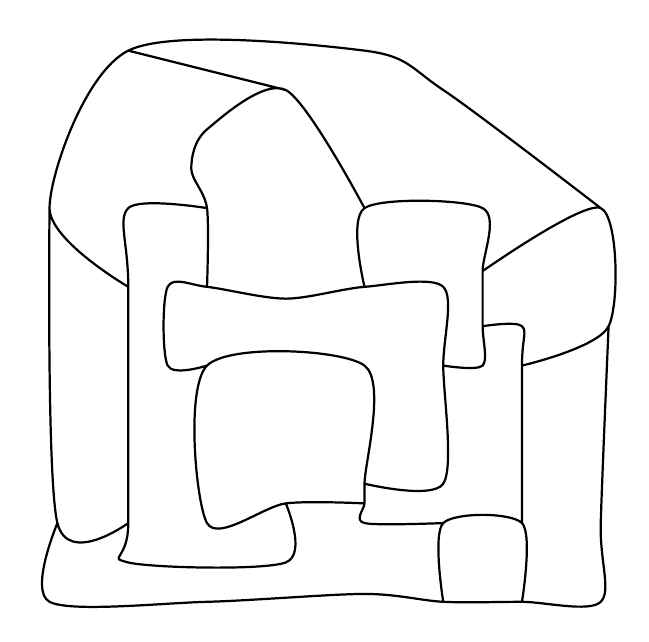
\begin{tikzpicture}
\draw[thick]
	plot [smooth] coordinates {(0.1,1) (0,0) (2,0) (4,0.1) (5,0) (6,0) (7,0) (7,1) (7.1,3.5)}
	plot [smooth] coordinates {(1,1) (0.1,1) (0,5)}
	plot [smooth] coordinates {(2,5) (1,5) (1,4) (1,1) (1,.5) (3,.5) (3,1.25)}
	plot [smooth] coordinates {(5,0) (5,1) (6,1) (6,0)}
	plot [smooth] coordinates {(6,1) (6,3) (6,3.5) (5.5,3.5)}
	plot [smooth] coordinates {(5,1) (4,1) (4,1.25) (4,1.5) (4,3) (2,3) (2,1) (3,1.25) (4,1.25)}
	plot [smooth] coordinates {(4,1.5) (5,1.5) (5,3) (5,4) (4,4) (3,3.85) (2,4) (1.5,4) (1.5,3) (2,3)}
	plot [smooth] coordinates {(5,3) (5.5,3) (5.5,3.5) (5.5, 4.2) (5.5,5) (4,5) (4,4)}
	plot [smooth] coordinates {(6,3) (7.1, 3.5) (7,5) (5.5,4.2)}
	plot [smooth] coordinates {(7,5) (5,6.5) (4,7) (1,7) (0,5) (1,4)}
	plot [smooth] coordinates {(2,4) (2,5) (1.8,5.5) (2,6) (3,6.5) (4,5)}
	plot [smooth] coordinates {(1,7) (3,6.5)};
\end{tikzpicture}
\end{center}

\end{activity}

Perhaps the most famous graph theory problem is how to color maps.

\begin{quote}
 Given any map of countries, states, counties, etc., how many colors are needed to color each region on the map so that neighboring regions are colored differently?
\end{quote}

Actual map makers usually use around seven colors.  For one thing, they require watery regions to be a specific color, and with a lot of colors it is easier to find a permissible coloring.  We want to know whether there is a smaller palette that will work for any map.

How is this related to graph theory?  Well, if we place a vertex in the center of each region (say in the capital of each state) and then connect two vertices if their states share a border, we get a graph.  Coloring regions on the map corresponds to coloring the vertices of the graph.  Since neighboring regions cannot be colored the same, our graph cannot have vertices colored the same when those vertices are adjacent.

In general, given any graph $G$, a coloring of the vertices is called (not surprisingly) a \emph{vertex coloring}\index{vertex coloring}\index{coloring}.  If the vertex coloring has the property that adjacent vertices are colored differently, then the coloring is called \emph{proper}.  Every graph has a proper vertex coloring.  For example, you could color every vertex with a different color.  But often you can do better.  The smallest number of colors needed to get a proper vertex coloring is called the \emph{chromatic number}\index{chromatic number} of the graph, written \gls{chiG}.

\begin{example}
  Find the chromatic number of the graphs below.
  \begin{center}
    \hfill
    \begin{tikzpicture}
      \foreach \x in {0,...,6}
      \draw  (\x*60:1) \v -- (\x*60+60:1) -- (\x*60+180:1) -- cycle;
    \end{tikzpicture}
    \hfill
    \begin{tikzpicture}[yscale=.8]
      \draw  (-1,0) \v -- (0,0) \v -- (1,0) \v -- (.5,1) \v -- (0,0) -- (-.5,1) \v -- (0,2) \v -- (.5,1) -- (-.5,1) -- (-1,0);
    \end{tikzpicture}
    \hfill
    \begin{tikzpicture}[yscale=.8, xscale=1.5]
 \draw  (-1, 0) \v -- (-.5,2) \v -- (0,0) \v -- (.5, 2) \v -- (1,0) \v -- (-.5,2) (.5,2) -- (-1,0);
  \end{tikzpicture}
  \hfill ~
  \end{center}

\begin{solution}
  The graph on the left is $K_6$.  The only way to properly color the graph is to give every vertex a different color (since every vertex is adjacent to every other vertex).  Thus the chromatic number is 6.

  The middle graph can be properly colored with just 3 colors (Red, Blue, and Green).  For example:

  \begin{center}
        \begin{tikzpicture}[yscale=.8]
      \draw  (-1,0) \vb{R} -- (0,0) \vb{B} -- (1,0) \vb{G} -- (.5,1) \vr{R} -- (0,0) -- (-.5,1) \vl{G} -- (0,2) \va{B} -- (.5,1) -- (-.5,1) -- (-1,0);
    \end{tikzpicture}
  \end{center}

  There is no way to color it with just two colors, since there are three vertices mutually adjacent (i.e., a triangle).  Thus the chromatic number is 3.

  The graph on the right is just $K_{2,3}$.  As with all bipartite graphs, this graph has chromatic number 2.   Color the vertices on the top row red and the vertices on the bottom row blue.
\end{solution}

\end{example}

It appears that there is no limit to how large chromatic numbers can get.  It should not come as a surprise that $K_n$ has chromatic number $n$.  So how could there possibly be an answer to the original map coloring question?  If the chromatic number of graph can be arbitrarily large, then it seems like there would be no upper bound to the number of colors needed for any map.  But there is.

The key observation is that while it is true that for any number $n$, there is a graph with chromatic number $n$, only some graphs arrive as representations of maps.  If you convert a map to a graph, the edges between vertices correspond to borders between the countries.  So you should be able to connect vertices in such a way where the edges do not cross.  In other words, the graphs representing maps are all {\em planar}!

So the question is, what is the largest chromatic number of any planar graph?  The answer is one of the best known theorems of mathematics:

\begin{theorem}[The Four Color Theorem\index{Four Color Theorem}]
If $G$ is a planar graph, then the chromatic number of $G$ is less than or equal to 4.  Thus any map can be properly colored with 4 or fewer colors.
\end{theorem}

We will not prove this theorem.  Really.  Even though the theorem is easy to state and understand, the proof is not.  In fact, there is currently no ``easy'' known proof of the theorem.  The current best proof still requires powerful computers to check an {\em unavoidable set} of  633 {\em reducible configurations}.  The idea is that every graph must contain one of these reducible configurations (this fact also needs to be checked by a computer) and that reducible configurations can, in fact, be colored in 4 or fewer colors.


\subsection{Coloring in General}
\begin{activity}
The math department plans to offer 10 classes next semester.  Some classes cannot run at the same time (perhaps they are taught by the same professor, or are required for seniors).

\begin{center}
\begin{tabular}{cl}
\textbf{Class:} & \textbf{Conflicts with:} \\ \hline
A & D I \\
B & D I J \\
C & E F I \\
D & A B F \\
E & H I\\
F & I\\
G & J \\
H & E I J\\
I & A B C E F H \\
J & B G H
\end{tabular}
\end{center}

How many different time slots are needed to teach these classes (and which should be taught at the same time)?  More importantly, how could we use graph coloring to answer this question?
\end{activity}


Cartography is certainly not the only application of graph coloring.  There are plenty of situations in which you might wish partition the objects in question so that related objects are not in the same set.  For example, you might wish to store chemicals safely.  To avoid explosions, certain pairs of chemicals should not be stored in the same room.  By coloring a graph (with vertices representing chemicals and edges representing potential negative interactions), you can determine the smallest number of rooms needed to store the chemicals.

Here is a further example:

\begin{example}
Radio stations broadcast their signal at certain frequencies.  However, there are a limited number of frequencies to choose from, so nationwide many stations use the same frequency.  This works because the stations are far enough apart that their signals will not interfere; no one radio could pick them up at the same time.

Suppose 10 new radio stations are to be set up in a currently unpopulated (by radio stations) region.  The radio stations that are close enough to each other to cause interference are recorded in the table below.  What is the fewest number of frequencies the stations could use.

\centerline{\begin{tabular}{c|c|c|c|c|c|c|c|c|c|c|}
 & {\tiny KQEA}&{\tiny KQEB}&{\tiny KQEC}&{\tiny KQED}&{\tiny KQEE}&{\tiny KQEF}&{\tiny KQEG}&{\tiny  KQEH}&{\tiny  KQEI}&{\tiny KQEJ } \\ \hline
{\tiny KQEA }&      &      &   x  &      &      &   x  &   x  &      &      &  x   \\ \hline
{\tiny KQEB }&      &      &   x  &   x  &      &      &      &      &      &      \\ \hline
{\tiny KQEC }&   x  &      &      &      &      &   x  &   x  &      &      &  x   \\ \hline
{\tiny KQED }&      &  x   &      &      &  x   &  x   &      &  x   &      &      \\ \hline
{\tiny KQEE }&      &      &      &  x   &      &      &      &      &  x   &      \\ \hline
{\tiny KQEF }&  x   &      &  x   &  x   &      &      &   x  &      &      &  x   \\ \hline
{\tiny KQEG }&  x   &      &  x   &      &      &  x   &      &      &      &  x   \\ \hline
{\tiny KQEH }&      &      &      &  x   &      &      &      &      &  x   &      \\ \hline
{\tiny KQEI }&      &      &      &      &  x   &      &      &  x   &      &  x   \\ \hline
{\tiny KQEJ }&  x   &      &  x   &      &      &  x   &   x  &      &  x   &      \\ \hline
\end{tabular}}

\begin{solution}
Represent the problem as a graph with vertices as the stations and edges when two stations are close enough to cause interference.  We are looking for the chromatic number of the graph.  Vertices that are colored identically represent stations that can have the same frequency.

This graph has chromatic number 5.  A proper 5-coloring is shown on the right.  Notice that the graph contains a copy of the complete graph $K_5$ so no fewer than 5 colors can be used.

\begin{center}
\begin{tikzpicture}[scale=.9]
\coordinate (A) at (90:2);
\coordinate (B) at (90-36:2);
\coordinate (C) at (90-2*36:2);
\coordinate (D) at (90-3*36:2);
\coordinate (E) at (90-4*36:2);
\coordinate (F) at (90-5*36:2);
\coordinate (G) at (90-6*36:2);
\coordinate (H) at (90-7*36:2);
\coordinate (I) at (90-8*36:2);
\coordinate (J) at (90-9*36:2);

\draw (A) -- (F) -- (D) -- (H) -- (I) (G) -- (J) -- (C) -- (F) (C) -- (G) -- (A) -- (J);

\draw (A) \va{\tiny KQEA} -- (C) \vr{\tiny KQEC} -- (B) \va{\tiny KQEB} -- (D) \vr{\tiny KQED} -- (E) \vb{\tiny KQEE} -- (I) \vl{\tiny KQEI} -- (J) \va{\tiny KQEJ} -- (F) \vb{\tiny KQEF} -- (G) \vl{\tiny KQEG} (H) \vl{\tiny KQEH};
\end{tikzpicture}
\qquad \qquad
\begin{tikzpicture}[scale=.9]
\coordinate (A) at (90:2);
\coordinate (B) at (90-36:2);
\coordinate (C) at (90-2*36:2);
\coordinate (D) at (90-3*36:2);
\coordinate (E) at (90-4*36:2);
\coordinate (F) at (90-5*36:2);
\coordinate (G) at (90-6*36:2);
\coordinate (H) at (90-7*36:2);
\coordinate (I) at (90-8*36:2);
\coordinate (J) at (90-9*36:2);

\draw (A) -- (F) -- (D) -- (H) -- (I) (G) -- (J) -- (C) -- (F) (C) -- (G) -- (A) -- (J);
\draw[line width=1.25pt] (A) -- (C) -- (F) -- (G) -- (J) -- (A) -- (F) -- (J) -- (C) -- (G) -- (A);

\draw (A) \va{\tiny R} -- (C) \vr{\tiny B} -- (B) \va{\tiny G} -- (D) \vr{\tiny B} -- (E) \vb{\tiny G} -- (I) \vl{\tiny B} -- (J) \va{\tiny P} -- (F) \vb{\tiny G} -- (G) \vl{\tiny Y} (H) \vl{\tiny R};
\end{tikzpicture}

\end{center}

\end{solution}
\end{example}

%\begin{example}
%Your high school chemistry teacher is getting a new lab.  She will need cabinets to store various chemicals.  To avoid explosions, it is important that some pairs of chemicals are definitely not stored in the same cabinet.   What is the fewest number of cabinets the chemist can use to store these chemicals?
%
%\begin{solution}
%
%\end{solution}
%\end{example}

In the example above, the chromatic number was 5, but this is not a counter-example to the Four Color Theorem, since the graph representing the radio stations is not planar.  It would be nice to have some quick way to find the chromatic number of a (possibly non-planar) graph.  It turns out nobody knows whether an efficient algorithm for computing chromatic numbers exists.

While we might not be able to find the exact chromatic number of graph easily, we can often give a reasonable range for the chromatic number.  In other words, we can give upper and lower bounds for chromatic number.

This is actually not very difficult: for every graph $G$, the chromatic number of $G$ is at least 1 and at most the number of vertices of $G$.

What?  You want \emph{better} bounds on the chromatic number?  Well you are in luck.

A \emph{clique}\index{clique} in a graph is a set of vertices all of which are pairwise adjacent.  In other words, a clique of size $n$ is just a copy of the complete graph $K_n$.  We define the \emph{clique number} of a graph to be the largest $n$ for which the graph contains a clique of size $n$.  Any clique of size $n$ cannot be colored with fewer than $n$ colors, so we have a nice lower bound:

\begin{theorem}
The chromatic number of a graph $G$ is at least the clique number of $G$.
\end{theorem}

There are times when the chromatic number of $G$ is \emph{equal} to the clique number.  These graphs have a special name -- they are called \emph{perfect}\index{perfect graph}.  If you know that a graph is perfect, then finding the chromatic number is simply a matter of searching for the largest clique.\footnote{There are special classes of graphs which can be proved to be perfect.  One such class is the set of \emph{chordal} graphs, which have the property that every cycle in the graph contains a \emph{chord} -- an edge between two vertices in of the cycle which are not adjacent in the cycle.}  However, not all graphs are perfect.

For an upper bound, we can improve on ``the number of vertices'' by looking to the degrees of vertices.  Let \gls{deltaG} be the largest degree of any vertex in the graph $G$.  One reasonable guess for an upper bound on the chromatic number is $\chi(G) \le \Delta(G) + 1$.  Why is this reasonable?  Starting with any vertex, it together with all of its neighbors can always be colored in $\Delta(G) + 1$ colors, since at most we are talking about $\Delta(G) + 1$ vertices in this set.  Now fan out!  At any point, if you consider an already colored vertex, some of its neighbors might be colored, some might not.  But no matter what, that vertex and its neighbors could all be colored distinctly, since there are at most $\Delta(G)$ neighbors, plus the one vertex being considered.

In fact, there are examples of graphs for which $\chi(G) = \Delta(G) + 1$.  For any $n$, the complete graph $K_n$ has chromatic number $n$, but $\Delta(K_n) = n-1$ (since every vertex is adjacent to every \emph{other} vertex).  Additionally, any \emph{odd} cycle will have chromatic number 3, but the degree of every vertex in a cycle is 2.  It turns out that these are the only two types of examples where we get equality, a result known as Brooks' Theorem.

\begin{theorem}[Brooks' Theorem\index{Brooks' Theorem}]
Any graph $G$ with maximal degree $\Delta(G)$ satisfies $\chi(G) \le \Delta(G)$, unless $G$ is a complete graph or an odd cycle, in which case $\chi(G) = \Delta(G) + 1$.
\end{theorem}

The proof of this theorem is \emph{just} complicated enough that we will not present it here (although you are asked to prove a special case in the exercises).  The adventurous reader is encouraged to find a book on graph theory for suggestions on how to prove the theorem.



%\begin{activity}
%A \emph{proper vertex coloring} of a graph is a coloring in which no two adjacent vertices are colored the same color.  The \emph{chromatic number} of a graph is the smallest number of colors needed for a proper coloring of the graph.
%
%For each graph below, find a proper coloring and determine the chromatic number of the graph.  As you are working on these colorings, think about the following ideas:
%\begin{enumerate}
%\item Before I even start coloring the graph, can I come up with an upper bound on the number of colors I will need (a bound that is better than simply the total number of vertices in the graph)?
%
%\item Before I even start coloring the graph, can I come up with a lower bound on the number of colors I will need (a bound that is better than simply 2)?
%
%\item Once you have colored the graph, make sure that you check your coloring with your tablemates to try to determine if you used the minimal number of colors.  Talk with each other about reasons why you couldn't have used fewer colors than you did.
%
%\item For each graph, try to identify if it is a type of graph that we've talked about before (i.e.\ does it have a special name or special properties).  If the graph is a named graph, try to see if you can generalize the ideas you used in your coloring of this graph to other graphs of that same type.
%\end{enumerate}
%
%ADD GRAPHS!
%
%\end{activity}\todo{Replace this with a map coloring question}



\subsection{Coloring Edges}


The chromatic number of a graph tells us about coloring vertices, but we could also ask about coloring edges.  Just like with vertex coloring, we might insist that edges that are adjacent must be colored differently.  Here, we are thinking of two edges as being adjacent if they are incident to the same vertex.  The least number of colors required to properly color the edges of a graph $G$ is called the \emph{chromatic index}\index{chromatic index} of $G$, written \gls{chiindG}.

\begin{example}
Six friends decide to spend the afternoon playing chess.  Everyone will play everyone else once.  They have plenty of chess sets but nobody wants to play more than one game at a time.  Games will last an hour (thanks to their handy chess clocks).  How many hours will the tournament last?

\begin{solution}
Represent each player with a vertex and put an edge between two players if they will play each other.  In this case, we get the graph $K_6$:

\begin{center}
\begin{tikzpicture}
\foreach \x in {0,...,5}{

	\foreach \y in {1,...,5}{
	 \draw (\x*60:1) -- (\x*60+\y*60:1);
	}
\draw (\x*60:1) \v;
}
\end{tikzpicture}
\end{center}

We must color the edges; each color represents a different hour.  Since different edges incident to the same vertex will be colored differently, no player will be playing two different games (edges) at the same time.  Thus we need to know the chromatic index of $K_6$.

Notice that for sure $\chi'(K_6) \ge 5$, since there is a vertex of degree 5. It turns out 5 colors is enough (go find such a coloring).  Therefore the friends will play for 5 hours.
\end{solution}
\end{example}

Interestingly, if one of the friends in the above example left, the remaining 5 chess-letes would still need 5 hours: the chromatic index of $K_5$ is also 5.

In general, what can we say about chromatic index?  Certainly $\chi'(G) \ge \Delta(G)$.  But how much higher could it be?  Only a little higher.

\begin{theorem}[Vizing's Theorem\index{Vizing's Theorem}]
For any graph $G$, the chromatic index $\chi'(G)$ is either $\Delta(G)$ or $\Delta(G) + 1$.
\end{theorem}

At first this theorem makes it seem like chromatic index might not be very interesting.  However, deciding which case a graph is in is not always easy.  Graphs for which $\chi'(G) = \Delta(G)$ are called \emph{class 1}, while the others are called \emph{class 2}. Bipartite graphs always satisfy $\chi'(G) = \Delta(G)$, so are class 1 (this was proved by K\"onig in 1916, decades before Vizing proved his theorem in 1964).  In 1965 Vizing proved that all planar graphs with $\Delta(G) \ge 8$ are of class 1, but this does not hold for all planar graphs with $2 \le \Delta(G) \le 5$.  Vizing conjectured that all planar graphs with $\Delta(G) = 6$ or $\Delta(G) = 7$ are class 1; the $\Delta(G) = 7$ case was proved in 2001 by Sanders and Zhao; the $\Delta(G) = 6$ case is still open.


There is another interesting way we might consider coloring edges, quite different from what we have discussed so far.  What if we colored every edge of a graph either red or blue.  Can we do so without, say, creating a \emph{monochromatic}\index{monochromatic} triangle (i.e., an all red or all blue triangle)?  Certainly for some graphs the answer is yes. Try doing so for $K_4$.  What about $K_5$?  $K_6$?  How far can we go?

The answer to the above problem is known and is a fun problem to do as an exercise.  We could extend the question in a variety of ways.  What if we had three colors?  What if we were trying to avoid other graphs.  The surprising fact is that very little is known about these questions.  For example, we know that you need to go up to $K_{17}$ in order to force a monochromatic triangle using three colors, but nobody knows how big you need to go with more colors.  Similarly, we know that using two colors $K_{18}$ is the smallest graph that forces a monochromatic copy of $K_4$, but the best we have to force a monochromatic $K_{5}$ is a range, somewhere from $K_{43}$ to $K_{49}$.  If you are interested in these sorts of questions, this area of graph theory is called Ramsey theory\index{Ramsey theory}.  Check it out.


\end{document}

	\withanswers\documentclass[12pt]{article}

\usepackage{discrete}

\def\thetitle{Introduction to Graph Theory} % will be put in the center header on the first page only.
\def\lefthead{Math 228 Notes} % will be put in the left header
\def\righthead{\thetitle} % will be put in the right header



\begin{document}


\section{Coloring}\label{sec:coloring}

\begin{activity}
Mapmakers in the fictional land of Euleria have drawn the borders of the various dukedoms of the land.  To make the map pretty, they wish to color each region.  Adjacent regions must be colored differently, but it is perfectly fine to color two distant regions with the same color.  What is the fewest colors the mapmakers can use and still accomplish this task?

\begin{center}
\begin{tikzpicture}
\draw[thick]
	plot [smooth] coordinates {(0.1,1) (0,0) (2,0) (4,0.1) (5,0) (6,0) (7,0) (7,1) (7.1,3.5)}
	plot [smooth] coordinates {(1,1) (0.1,1) (0,5)}
	plot [smooth] coordinates {(2,5) (1,5) (1,4) (1,1) (1,.5) (3,.5) (3,1.25)}
	plot [smooth] coordinates {(5,0) (5,1) (6,1) (6,0)}
	plot [smooth] coordinates {(6,1) (6,3) (6,3.5) (5.5,3.5)}
	plot [smooth] coordinates {(5,1) (4,1) (4,1.25) (4,1.5) (4,3) (2,3) (2,1) (3,1.25) (4,1.25)}
	plot [smooth] coordinates {(4,1.5) (5,1.5) (5,3) (5,4) (4,4) (3,3.85) (2,4) (1.5,4) (1.5,3) (2,3)}
	plot [smooth] coordinates {(5,3) (5.5,3) (5.5,3.5) (5.5, 4.2) (5.5,5) (4,5) (4,4)}
	plot [smooth] coordinates {(6,3) (7.1, 3.5) (7,5) (5.5,4.2)}
	plot [smooth] coordinates {(7,5) (5,6.5) (4,7) (1,7) (0,5) (1,4)}
	plot [smooth] coordinates {(2,4) (2,5) (1.8,5.5) (2,6) (3,6.5) (4,5)}
	plot [smooth] coordinates {(1,7) (3,6.5)};
\end{tikzpicture}
\end{center}

\end{activity}

Perhaps the most famous graph theory problem is how to color maps.

\begin{quote}
 Given any map of countries, states, counties, etc., how many colors are needed to color each region on the map so that neighboring regions are colored differently?
\end{quote}

Actual map makers usually use around seven colors.  For one thing, they require watery regions to be a specific color, and with a lot of colors it is easier to find a permissible coloring.  We want to know whether there is a smaller palette that will work for any map.

How is this related to graph theory?  Well, if we place a vertex in the center of each region (say in the capital of each state) and then connect two vertices if their states share a border, we get a graph.  Coloring regions on the map corresponds to coloring the vertices of the graph.  Since neighboring regions cannot be colored the same, our graph cannot have vertices colored the same when those vertices are adjacent.

In general, given any graph $G$, a coloring of the vertices is called (not surprisingly) a \emph{vertex coloring}\index{vertex coloring}\index{coloring}.  If the vertex coloring has the property that adjacent vertices are colored differently, then the coloring is called \emph{proper}.  Every graph has a proper vertex coloring.  For example, you could color every vertex with a different color.  But often you can do better.  The smallest number of colors needed to get a proper vertex coloring is called the \emph{chromatic number}\index{chromatic number} of the graph, written \gls{chiG}.

\begin{example}
  Find the chromatic number of the graphs below.
  \begin{center}
    \hfill
    \begin{tikzpicture}
      \foreach \x in {0,...,6}
      \draw  (\x*60:1) \v -- (\x*60+60:1) -- (\x*60+180:1) -- cycle;
    \end{tikzpicture}
    \hfill
    \begin{tikzpicture}[yscale=.8]
      \draw  (-1,0) \v -- (0,0) \v -- (1,0) \v -- (.5,1) \v -- (0,0) -- (-.5,1) \v -- (0,2) \v -- (.5,1) -- (-.5,1) -- (-1,0);
    \end{tikzpicture}
    \hfill
    \begin{tikzpicture}[yscale=.8, xscale=1.5]
 \draw  (-1, 0) \v -- (-.5,2) \v -- (0,0) \v -- (.5, 2) \v -- (1,0) \v -- (-.5,2) (.5,2) -- (-1,0);
  \end{tikzpicture}
  \hfill ~
  \end{center}

\begin{solution}
  The graph on the left is $K_6$.  The only way to properly color the graph is to give every vertex a different color (since every vertex is adjacent to every other vertex).  Thus the chromatic number is 6.

  The middle graph can be properly colored with just 3 colors (Red, Blue, and Green).  For example:

  \begin{center}
        \begin{tikzpicture}[yscale=.8]
      \draw  (-1,0) \vb{R} -- (0,0) \vb{B} -- (1,0) \vb{G} -- (.5,1) \vr{R} -- (0,0) -- (-.5,1) \vl{G} -- (0,2) \va{B} -- (.5,1) -- (-.5,1) -- (-1,0);
    \end{tikzpicture}
  \end{center}

  There is no way to color it with just two colors, since there are three vertices mutually adjacent (i.e., a triangle).  Thus the chromatic number is 3.

  The graph on the right is just $K_{2,3}$.  As with all bipartite graphs, this graph has chromatic number 2.   Color the vertices on the top row red and the vertices on the bottom row blue.
\end{solution}

\end{example}

It appears that there is no limit to how large chromatic numbers can get.  It should not come as a surprise that $K_n$ has chromatic number $n$.  So how could there possibly be an answer to the original map coloring question?  If the chromatic number of graph can be arbitrarily large, then it seems like there would be no upper bound to the number of colors needed for any map.  But there is.

The key observation is that while it is true that for any number $n$, there is a graph with chromatic number $n$, only some graphs arrive as representations of maps.  If you convert a map to a graph, the edges between vertices correspond to borders between the countries.  So you should be able to connect vertices in such a way where the edges do not cross.  In other words, the graphs representing maps are all {\em planar}!

So the question is, what is the largest chromatic number of any planar graph?  The answer is one of the best known theorems of mathematics:

\begin{theorem}[The Four Color Theorem\index{Four Color Theorem}]
If $G$ is a planar graph, then the chromatic number of $G$ is less than or equal to 4.  Thus any map can be properly colored with 4 or fewer colors.
\end{theorem}

We will not prove this theorem.  Really.  Even though the theorem is easy to state and understand, the proof is not.  In fact, there is currently no ``easy'' known proof of the theorem.  The current best proof still requires powerful computers to check an {\em unavoidable set} of  633 {\em reducible configurations}.  The idea is that every graph must contain one of these reducible configurations (this fact also needs to be checked by a computer) and that reducible configurations can, in fact, be colored in 4 or fewer colors.


\subsection{Coloring in General}
\begin{activity}
The math department plans to offer 10 classes next semester.  Some classes cannot run at the same time (perhaps they are taught by the same professor, or are required for seniors).

\begin{center}
\begin{tabular}{cl}
\textbf{Class:} & \textbf{Conflicts with:} \\ \hline
A & D I \\
B & D I J \\
C & E F I \\
D & A B F \\
E & H I\\
F & I\\
G & J \\
H & E I J\\
I & A B C E F H \\
J & B G H
\end{tabular}
\end{center}

How many different time slots are needed to teach these classes (and which should be taught at the same time)?  More importantly, how could we use graph coloring to answer this question?
\end{activity}


Cartography is certainly not the only application of graph coloring.  There are plenty of situations in which you might wish partition the objects in question so that related objects are not in the same set.  For example, you might wish to store chemicals safely.  To avoid explosions, certain pairs of chemicals should not be stored in the same room.  By coloring a graph (with vertices representing chemicals and edges representing potential negative interactions), you can determine the smallest number of rooms needed to store the chemicals.

Here is a further example:

\begin{example}
Radio stations broadcast their signal at certain frequencies.  However, there are a limited number of frequencies to choose from, so nationwide many stations use the same frequency.  This works because the stations are far enough apart that their signals will not interfere; no one radio could pick them up at the same time.

Suppose 10 new radio stations are to be set up in a currently unpopulated (by radio stations) region.  The radio stations that are close enough to each other to cause interference are recorded in the table below.  What is the fewest number of frequencies the stations could use.

\centerline{\begin{tabular}{c|c|c|c|c|c|c|c|c|c|c|}
 & {\tiny KQEA}&{\tiny KQEB}&{\tiny KQEC}&{\tiny KQED}&{\tiny KQEE}&{\tiny KQEF}&{\tiny KQEG}&{\tiny  KQEH}&{\tiny  KQEI}&{\tiny KQEJ } \\ \hline
{\tiny KQEA }&      &      &   x  &      &      &   x  &   x  &      &      &  x   \\ \hline
{\tiny KQEB }&      &      &   x  &   x  &      &      &      &      &      &      \\ \hline
{\tiny KQEC }&   x  &      &      &      &      &   x  &   x  &      &      &  x   \\ \hline
{\tiny KQED }&      &  x   &      &      &  x   &  x   &      &  x   &      &      \\ \hline
{\tiny KQEE }&      &      &      &  x   &      &      &      &      &  x   &      \\ \hline
{\tiny KQEF }&  x   &      &  x   &  x   &      &      &   x  &      &      &  x   \\ \hline
{\tiny KQEG }&  x   &      &  x   &      &      &  x   &      &      &      &  x   \\ \hline
{\tiny KQEH }&      &      &      &  x   &      &      &      &      &  x   &      \\ \hline
{\tiny KQEI }&      &      &      &      &  x   &      &      &  x   &      &  x   \\ \hline
{\tiny KQEJ }&  x   &      &  x   &      &      &  x   &   x  &      &  x   &      \\ \hline
\end{tabular}}

\begin{solution}
Represent the problem as a graph with vertices as the stations and edges when two stations are close enough to cause interference.  We are looking for the chromatic number of the graph.  Vertices that are colored identically represent stations that can have the same frequency.

This graph has chromatic number 5.  A proper 5-coloring is shown on the right.  Notice that the graph contains a copy of the complete graph $K_5$ so no fewer than 5 colors can be used.

\begin{center}
\begin{tikzpicture}[scale=.9]
\coordinate (A) at (90:2);
\coordinate (B) at (90-36:2);
\coordinate (C) at (90-2*36:2);
\coordinate (D) at (90-3*36:2);
\coordinate (E) at (90-4*36:2);
\coordinate (F) at (90-5*36:2);
\coordinate (G) at (90-6*36:2);
\coordinate (H) at (90-7*36:2);
\coordinate (I) at (90-8*36:2);
\coordinate (J) at (90-9*36:2);

\draw (A) -- (F) -- (D) -- (H) -- (I) (G) -- (J) -- (C) -- (F) (C) -- (G) -- (A) -- (J);

\draw (A) \va{\tiny KQEA} -- (C) \vr{\tiny KQEC} -- (B) \va{\tiny KQEB} -- (D) \vr{\tiny KQED} -- (E) \vb{\tiny KQEE} -- (I) \vl{\tiny KQEI} -- (J) \va{\tiny KQEJ} -- (F) \vb{\tiny KQEF} -- (G) \vl{\tiny KQEG} (H) \vl{\tiny KQEH};
\end{tikzpicture}
\qquad \qquad
\begin{tikzpicture}[scale=.9]
\coordinate (A) at (90:2);
\coordinate (B) at (90-36:2);
\coordinate (C) at (90-2*36:2);
\coordinate (D) at (90-3*36:2);
\coordinate (E) at (90-4*36:2);
\coordinate (F) at (90-5*36:2);
\coordinate (G) at (90-6*36:2);
\coordinate (H) at (90-7*36:2);
\coordinate (I) at (90-8*36:2);
\coordinate (J) at (90-9*36:2);

\draw (A) -- (F) -- (D) -- (H) -- (I) (G) -- (J) -- (C) -- (F) (C) -- (G) -- (A) -- (J);
\draw[line width=1.25pt] (A) -- (C) -- (F) -- (G) -- (J) -- (A) -- (F) -- (J) -- (C) -- (G) -- (A);

\draw (A) \va{\tiny R} -- (C) \vr{\tiny B} -- (B) \va{\tiny G} -- (D) \vr{\tiny B} -- (E) \vb{\tiny G} -- (I) \vl{\tiny B} -- (J) \va{\tiny P} -- (F) \vb{\tiny G} -- (G) \vl{\tiny Y} (H) \vl{\tiny R};
\end{tikzpicture}

\end{center}

\end{solution}
\end{example}

%\begin{example}
%Your high school chemistry teacher is getting a new lab.  She will need cabinets to store various chemicals.  To avoid explosions, it is important that some pairs of chemicals are definitely not stored in the same cabinet.   What is the fewest number of cabinets the chemist can use to store these chemicals?
%
%\begin{solution}
%
%\end{solution}
%\end{example}

In the example above, the chromatic number was 5, but this is not a counter-example to the Four Color Theorem, since the graph representing the radio stations is not planar.  It would be nice to have some quick way to find the chromatic number of a (possibly non-planar) graph.  It turns out nobody knows whether an efficient algorithm for computing chromatic numbers exists.

While we might not be able to find the exact chromatic number of graph easily, we can often give a reasonable range for the chromatic number.  In other words, we can give upper and lower bounds for chromatic number.

This is actually not very difficult: for every graph $G$, the chromatic number of $G$ is at least 1 and at most the number of vertices of $G$.

What?  You want \emph{better} bounds on the chromatic number?  Well you are in luck.

A \emph{clique}\index{clique} in a graph is a set of vertices all of which are pairwise adjacent.  In other words, a clique of size $n$ is just a copy of the complete graph $K_n$.  We define the \emph{clique number} of a graph to be the largest $n$ for which the graph contains a clique of size $n$.  Any clique of size $n$ cannot be colored with fewer than $n$ colors, so we have a nice lower bound:

\begin{theorem}
The chromatic number of a graph $G$ is at least the clique number of $G$.
\end{theorem}

There are times when the chromatic number of $G$ is \emph{equal} to the clique number.  These graphs have a special name -- they are called \emph{perfect}\index{perfect graph}.  If you know that a graph is perfect, then finding the chromatic number is simply a matter of searching for the largest clique.\footnote{There are special classes of graphs which can be proved to be perfect.  One such class is the set of \emph{chordal} graphs, which have the property that every cycle in the graph contains a \emph{chord} -- an edge between two vertices in of the cycle which are not adjacent in the cycle.}  However, not all graphs are perfect.

For an upper bound, we can improve on ``the number of vertices'' by looking to the degrees of vertices.  Let \gls{deltaG} be the largest degree of any vertex in the graph $G$.  One reasonable guess for an upper bound on the chromatic number is $\chi(G) \le \Delta(G) + 1$.  Why is this reasonable?  Starting with any vertex, it together with all of its neighbors can always be colored in $\Delta(G) + 1$ colors, since at most we are talking about $\Delta(G) + 1$ vertices in this set.  Now fan out!  At any point, if you consider an already colored vertex, some of its neighbors might be colored, some might not.  But no matter what, that vertex and its neighbors could all be colored distinctly, since there are at most $\Delta(G)$ neighbors, plus the one vertex being considered.

In fact, there are examples of graphs for which $\chi(G) = \Delta(G) + 1$.  For any $n$, the complete graph $K_n$ has chromatic number $n$, but $\Delta(K_n) = n-1$ (since every vertex is adjacent to every \emph{other} vertex).  Additionally, any \emph{odd} cycle will have chromatic number 3, but the degree of every vertex in a cycle is 2.  It turns out that these are the only two types of examples where we get equality, a result known as Brooks' Theorem.

\begin{theorem}[Brooks' Theorem\index{Brooks' Theorem}]
Any graph $G$ with maximal degree $\Delta(G)$ satisfies $\chi(G) \le \Delta(G)$, unless $G$ is a complete graph or an odd cycle, in which case $\chi(G) = \Delta(G) + 1$.
\end{theorem}

The proof of this theorem is \emph{just} complicated enough that we will not present it here (although you are asked to prove a special case in the exercises).  The adventurous reader is encouraged to find a book on graph theory for suggestions on how to prove the theorem.



%\begin{activity}
%A \emph{proper vertex coloring} of a graph is a coloring in which no two adjacent vertices are colored the same color.  The \emph{chromatic number} of a graph is the smallest number of colors needed for a proper coloring of the graph.
%
%For each graph below, find a proper coloring and determine the chromatic number of the graph.  As you are working on these colorings, think about the following ideas:
%\begin{enumerate}
%\item Before I even start coloring the graph, can I come up with an upper bound on the number of colors I will need (a bound that is better than simply the total number of vertices in the graph)?
%
%\item Before I even start coloring the graph, can I come up with a lower bound on the number of colors I will need (a bound that is better than simply 2)?
%
%\item Once you have colored the graph, make sure that you check your coloring with your tablemates to try to determine if you used the minimal number of colors.  Talk with each other about reasons why you couldn't have used fewer colors than you did.
%
%\item For each graph, try to identify if it is a type of graph that we've talked about before (i.e.\ does it have a special name or special properties).  If the graph is a named graph, try to see if you can generalize the ideas you used in your coloring of this graph to other graphs of that same type.
%\end{enumerate}
%
%ADD GRAPHS!
%
%\end{activity}\todo{Replace this with a map coloring question}



\subsection{Coloring Edges}


The chromatic number of a graph tells us about coloring vertices, but we could also ask about coloring edges.  Just like with vertex coloring, we might insist that edges that are adjacent must be colored differently.  Here, we are thinking of two edges as being adjacent if they are incident to the same vertex.  The least number of colors required to properly color the edges of a graph $G$ is called the \emph{chromatic index}\index{chromatic index} of $G$, written \gls{chiindG}.

\begin{example}
Six friends decide to spend the afternoon playing chess.  Everyone will play everyone else once.  They have plenty of chess sets but nobody wants to play more than one game at a time.  Games will last an hour (thanks to their handy chess clocks).  How many hours will the tournament last?

\begin{solution}
Represent each player with a vertex and put an edge between two players if they will play each other.  In this case, we get the graph $K_6$:

\begin{center}
\begin{tikzpicture}
\foreach \x in {0,...,5}{

	\foreach \y in {1,...,5}{
	 \draw (\x*60:1) -- (\x*60+\y*60:1);
	}
\draw (\x*60:1) \v;
}
\end{tikzpicture}
\end{center}

We must color the edges; each color represents a different hour.  Since different edges incident to the same vertex will be colored differently, no player will be playing two different games (edges) at the same time.  Thus we need to know the chromatic index of $K_6$.

Notice that for sure $\chi'(K_6) \ge 5$, since there is a vertex of degree 5. It turns out 5 colors is enough (go find such a coloring).  Therefore the friends will play for 5 hours.
\end{solution}
\end{example}

Interestingly, if one of the friends in the above example left, the remaining 5 chess-letes would still need 5 hours: the chromatic index of $K_5$ is also 5.

In general, what can we say about chromatic index?  Certainly $\chi'(G) \ge \Delta(G)$.  But how much higher could it be?  Only a little higher.

\begin{theorem}[Vizing's Theorem\index{Vizing's Theorem}]
For any graph $G$, the chromatic index $\chi'(G)$ is either $\Delta(G)$ or $\Delta(G) + 1$.
\end{theorem}

At first this theorem makes it seem like chromatic index might not be very interesting.  However, deciding which case a graph is in is not always easy.  Graphs for which $\chi'(G) = \Delta(G)$ are called \emph{class 1}, while the others are called \emph{class 2}. Bipartite graphs always satisfy $\chi'(G) = \Delta(G)$, so are class 1 (this was proved by K\"onig in 1916, decades before Vizing proved his theorem in 1964).  In 1965 Vizing proved that all planar graphs with $\Delta(G) \ge 8$ are of class 1, but this does not hold for all planar graphs with $2 \le \Delta(G) \le 5$.  Vizing conjectured that all planar graphs with $\Delta(G) = 6$ or $\Delta(G) = 7$ are class 1; the $\Delta(G) = 7$ case was proved in 2001 by Sanders and Zhao; the $\Delta(G) = 6$ case is still open.


There is another interesting way we might consider coloring edges, quite different from what we have discussed so far.  What if we colored every edge of a graph either red or blue.  Can we do so without, say, creating a \emph{monochromatic}\index{monochromatic} triangle (i.e., an all red or all blue triangle)?  Certainly for some graphs the answer is yes. Try doing so for $K_4$.  What about $K_5$?  $K_6$?  How far can we go?

The answer to the above problem is known and is a fun problem to do as an exercise.  We could extend the question in a variety of ways.  What if we had three colors?  What if we were trying to avoid other graphs.  The surprising fact is that very little is known about these questions.  For example, we know that you need to go up to $K_{17}$ in order to force a monochromatic triangle using three colors, but nobody knows how big you need to go with more colors.  Similarly, we know that using two colors $K_{18}$ is the smallest graph that forces a monochromatic copy of $K_4$, but the best we have to force a monochromatic $K_{5}$ is a range, somewhere from $K_{43}$ to $K_{49}$.  If you are interested in these sorts of questions, this area of graph theory is called Ramsey theory\index{Ramsey theory}.  Check it out.


\end{document}


	\documentclass[12pt]{article}

\usepackage{discrete}

\def\thetitle{Introduction to Graph Theory} % will be put in the center header on the first page only.
\def\lefthead{Math 228 Notes} % will be put in the left header
\def\righthead{\thetitle} % will be put in the right header



\begin{document}

%Eventually I should change this language over to Euler ``tours'' to be more current.

\section{Euler Paths and Circuits}\label{sec:paths}



\begin{activity}
\noindent An Euler path, in a graph or multigraph, is a path which uses every edge exactly once.  An Euler circuit is an Euler path which starts and stops at the same vertex.  Our goal is to find a quick way to check whether a graph (or multigraph) has an Euler path or circuit.

\begin{questions}
\question Which of the graphs below have Euler paths?  Which have Euler circuits?


\begin{center}
 \begin{tikzpicture}[scale=0.9]
  \draw (-1,0) \v -- (1,0)\v -- (1,2) \v -- (-1, 2) \v -- (-1,0) -- (1,2) (-1,2) -- (1,0) (0,1) \v;
  \draw (-1,2) -- (0,3) \v -- (1,2);
\end{tikzpicture}
\hfill
 \begin{tikzpicture}[scale=0.9]
  \draw (-1,0) \v -- (1,0)\v -- (1,2) \v -- (-1, 2) \v -- (-1,0) -- (1,2) (-1,2) -- (1,0) (0,1) \v;
\end{tikzpicture}
\hfill
 \begin{tikzpicture}[scale=0.9]
  \draw (-1,0) \v -- (1,0)\v -- (1,2) \v -- (-1, 2) \v -- (-1,0) -- (1,2) (-1,2) -- (1,0) (0,1) \v;
  \draw (-1,0) -- (-2,1) \v -- (-1,2) (1,2) -- (2,1) \v -- (1,0);
\end{tikzpicture}
\hfill
\begin{tikzpicture}[yscale=.45]
 \draw (-1,-2) \v to [out=120, in=240] (-1,0) \v to [out=120, in=240] (-1,2) \v to [out=300, in=60] (-1,0) to [out=300, in=60] (-1,-2);
  \draw (1,0) \v -- (-1,2) (-1,0) -- (1,0) -- (-1,-2);
  \end{tikzpicture}

\end{center}



%\question What is the smallest number of bridges you must add to K\"onigsberg to get an Euler path?  What about an Euler circuit?
%
%\begin{center}
% \begin{tikzpicture}[yscale=.5, scale=1]
% \draw[thick] (-1,-2) \v to [out=120, in=240] (-1,0) \v to [out=120, in=240] (-1,2) \v to [out=300, in=60] (-1,0) to [out=300, in=60] (-1,-2);
%  \draw[thick] (1,0) \v -- (-1,2) (-1,0) -- (1,0) -- (-1,-2);
%  \end{tikzpicture}
%\end{center}




\question List the degrees of each vertex of the graphs above.  Is there a connection between degrees and the existence of Euler paths and circuits?

%\begin{center}
% \begin{tikzpicture}
%  \draw[thick] (-1,0) \v -- (1,0)\v -- (1,2) \v -- (-1, 2) \v -- (-1,0) -- (1,2) (-1,2) -- (1,0) (0,1) \v;
%  \draw[thick] (-1,2) -- (0,3) \v -- (1,2);
%\end{tikzpicture}
%\hfill
% \begin{tikzpicture}
%  \draw[thick] (-1,0) \v -- (1,0)\v -- (1,2) \v -- (-1, 2) \v -- (-1,0) -- (1,2) (-1,2) -- (1,0) (0,1) \v;
%\end{tikzpicture}
%\hfill
% \begin{tikzpicture}
%  \draw[thick] (-1,0) \v -- (1,0)\v -- (1,2) \v -- (-1, 2) \v -- (-1,0) -- (1,2) (-1,2) -- (1,0) (0,1) \v;
%  \draw[thick] (-1,0) -- (-2,1) \v -- (-1,2) (1,2) -- (2,1) \v -- (1,0);
%\end{tikzpicture}
%\hfill
%\begin{tikzpicture}[yscale=.5]
% \draw[thick] (-1,-2) \v to [out=120, in=240] (-1,0) \v to [out=120, in=240] (-1,2) \v to [out=300, in=60] (-1,0) to [out=300, in=60] (-1,-2);
%  \draw[thick] (1,0) \v -- (-1,2) (-1,0) -- (1,0) -- (-1,-2);
%  \end{tikzpicture}
%
%\end{center}
%


\question Is it possible for a graph with a degree 1 vertex to have an Euler circuit?  If so, draw one.  If not, explain why not.  What about an Euler path?


\question What if every vertex of the graph has degree 2.  Is there an Euler path?  An Euler circuit?  Draw some graphs.


\question Below is {\em part} of a graph.  Even though you can only see some of the vertices, can you deduce whether the graph will have an Euler path or circuit?

\begin{center}
 \begin{tikzpicture}[scale=0.9]
  \draw (-2,0) \v -- (0,1) \v -- (2,0) \v;
  \draw (-2,0) -- (-2.5, -.5) (-2,0) -- (-2, -.5) (-2,0) -- (-1.5,-.5);
  \draw[dashed] (-2.5, -.5) -- (-3, -1) (-2,-.5) -- (-2,-1) (-1.5,-.5) -- (-1,-1);
    \draw (2,0) -- (2.5, -.5) (2,0) -- (2, -.5) (2,0) -- (1.5,-.5);
  \draw[dashed] (2.5, -.5) -- (3, -1) (2,-.5) -- (2,-1) (1.5,-.5) -- (1,-1);
    \draw (0,1) -- (-.25, 0) (0,1) -- (0, 0) (0,1) -- (.25,0);
  \draw[dashed] (-.25, 0) -- (-.5, -1) (0,0) -- (0,-1) (.25,0) -- (.5,-1);
 \end{tikzpicture}

\end{center}
\end{questions}
\end{activity}



If we start at a vertex and trace along edges to get to other vertices, we create a {\em path} on the graph.  If the path travels along every edge exactly once, then the path is called an {\em Euler path} (or {\em Eulerian path}).  If, in addition, the starting and ending vertices are the same (so you trace along every edge exactly once and end up where you started), then the path is called an {\em Euler circuit}.  Of course if a graph is not connected, there is no hope of finding such a path or circuit.  For the rest of this section, assume all the graphs discussed are connected.

The bridges of K\"onigsberg problem is really a question about the existence of Euler paths.  There will be a route that crosses every bridge exactly once if and only if the graph below has an Euler path:

\centerline{\begin{tikzpicture}[scale=1, yscale=.5]
 \draw (-1,-2) \v to [out=120, in=240] (-1,0) \v to [out=120, in=240] (-1,2) \v to [out=300, in=60] (-1,0) to [out=300, in=60] (-1,-2);
  \draw (1,0) \v -- (-1,2) (-1,0) -- (1,0) -- (-1,-2);
  \end{tikzpicture}}

This graph is small enough that we could actually check every possible path and in doing so convince ourselves that there is no Euler path (let alone an Euler circuit).  On small graphs which do have an Euler path, it is usually not difficult to find one.  Our goal is to find a quick way to check whether a graph has an Euler path or circuit, even if the graph is quite large.

One way to guarantee that a graph does {\em not} have an Euler circuit is to include a ``spike,'' a vertex of degree 1.

\begin{center}
 \begin{tikzpicture}
  \draw (-1,0) \v -- (0,1) \v -- (1,0) \v -- cycle;
  \draw (0,1) -- (1,1) \v node[below right]{$a$};
 \end{tikzpicture}
\end{center}

The vertex $a$ has degree 1, and if you try to make an Euler circuit, you see that you will get stuck at the vertex.  It is a dead end.  That is, unless you start there.  But then there is no way to return, so there is no hope of finding an Euler circuit.  There is however an Euler path.  It starts at the vertex $a$, then loops around the triangle.  You will end at the vertex of degree 3.

You run into a similar problem whenever you have a vertex of any odd degree.  If you start at such a vertex, you will not be able to end there (after traversing every edge exactly once).  After using one edge to leave the starting vertex, you will be left with an even number of edges emanating from the vertex.  Half of these could be used for returning to the vertex, the other half for leaving.  So you return, then leave.  Return, then leave.  The only way to use up all the edges is to use the last one by leaving the vertex.  On the other hand, if you have a vertex with odd degree that you do not start a path at, then you will eventually get stuck at that vertex.  The path will use pairs of edges incident to the vertex to arrive and leave again.  Eventually all but one of these edges will be used up, leaving only an edge to arrive by, and none to leave again.

What all this says is that if a graph has an Euler path and two vertices with odd degree, then the Euler path must start at one of the odd degree vertices and end at the other.  In such a situation, every other vertex {\em must} have an even degree since we need an equal number of edges to get to those vertices as to leave them.  How could we have an Euler circuit?  The graph could not have any odd degree vertex as an Euler path would have to start there or end there, but not both.  Thus for a graph to have an Euler circuit, all vertices must have even degree.

The converse is also true: if all the vertices of a graph have even degree, then the graph has an Euler circuit, and if there are exactly two vertices with odd degree, the graph has an Euler path.  To prove this is a little tricky, but the basic idea is that you will never get stuck because there is an ``outbound'' edge for every ``inbound'' edge at every vertex.  If you try to make an Euler path and miss some edges, you will always be able to ``splice in'' a circuit using the edges you previously missed.

\begin{defbox}{Euler Paths and Circuits}
\begin{itemize}
 \item A graph has an Euler circuit if and only if the degree of every vertex is even.
 \item A graph has an Euler path if and only if there are at most two vertices with odd degree.
\end{itemize}

\end{defbox}

Since the bridges of K\"onigsberg graph has all four vertices with odd degree, there is no Euler path through the graph.

\subsection{Hamilton Paths}

Suppose you wanted to tour K\"onigsberg in such a way where you visit each land mass (the two islands and both banks) exactly once.  This can be done.  In graph theory terms, we are asking whether there is a path which visits every vertex exactly once.  Such a path is called a {\em Hamilton path} (or Hamiltonian path)\index{Hamilton path}.  It appears that finding Hamilton paths would be easier because graphs often have more edges than vertices, so there are fewer requirements to be met.  However, nobody knows whether this is true.  There is no known simple test for whether a graph has a Hamilton path.  For small graphs this is not a problem, but as the size of the graph grows, it gets harder and harder to check wither there is a Hamilton path.  In fact, this is an example of a question which as far as we know is too difficult for computers to solve; it is an example of a problem which is NP-complete\index{NP-complete}.



\end{document}

	\withanswers\documentclass[12pt]{article}

\usepackage{discrete}

\def\thetitle{Introduction to Graph Theory} % will be put in the center header on the first page only.
\def\lefthead{Math 228 Notes} % will be put in the left header
\def\righthead{\thetitle} % will be put in the right header



\begin{document}

%Eventually I should change this language over to Euler ``tours'' to be more current.

\section{Euler Paths and Circuits}\label{sec:paths}



\begin{activity}
\noindent An Euler path, in a graph or multigraph, is a path which uses every edge exactly once.  An Euler circuit is an Euler path which starts and stops at the same vertex.  Our goal is to find a quick way to check whether a graph (or multigraph) has an Euler path or circuit.

\begin{questions}
\question Which of the graphs below have Euler paths?  Which have Euler circuits?


\begin{center}
 \begin{tikzpicture}[scale=0.9]
  \draw (-1,0) \v -- (1,0)\v -- (1,2) \v -- (-1, 2) \v -- (-1,0) -- (1,2) (-1,2) -- (1,0) (0,1) \v;
  \draw (-1,2) -- (0,3) \v -- (1,2);
\end{tikzpicture}
\hfill
 \begin{tikzpicture}[scale=0.9]
  \draw (-1,0) \v -- (1,0)\v -- (1,2) \v -- (-1, 2) \v -- (-1,0) -- (1,2) (-1,2) -- (1,0) (0,1) \v;
\end{tikzpicture}
\hfill
 \begin{tikzpicture}[scale=0.9]
  \draw (-1,0) \v -- (1,0)\v -- (1,2) \v -- (-1, 2) \v -- (-1,0) -- (1,2) (-1,2) -- (1,0) (0,1) \v;
  \draw (-1,0) -- (-2,1) \v -- (-1,2) (1,2) -- (2,1) \v -- (1,0);
\end{tikzpicture}
\hfill
\begin{tikzpicture}[yscale=.45]
 \draw (-1,-2) \v to [out=120, in=240] (-1,0) \v to [out=120, in=240] (-1,2) \v to [out=300, in=60] (-1,0) to [out=300, in=60] (-1,-2);
  \draw (1,0) \v -- (-1,2) (-1,0) -- (1,0) -- (-1,-2);
  \end{tikzpicture}

\end{center}



%\question What is the smallest number of bridges you must add to K\"onigsberg to get an Euler path?  What about an Euler circuit?
%
%\begin{center}
% \begin{tikzpicture}[yscale=.5, scale=1]
% \draw[thick] (-1,-2) \v to [out=120, in=240] (-1,0) \v to [out=120, in=240] (-1,2) \v to [out=300, in=60] (-1,0) to [out=300, in=60] (-1,-2);
%  \draw[thick] (1,0) \v -- (-1,2) (-1,0) -- (1,0) -- (-1,-2);
%  \end{tikzpicture}
%\end{center}




\question List the degrees of each vertex of the graphs above.  Is there a connection between degrees and the existence of Euler paths and circuits?

%\begin{center}
% \begin{tikzpicture}
%  \draw[thick] (-1,0) \v -- (1,0)\v -- (1,2) \v -- (-1, 2) \v -- (-1,0) -- (1,2) (-1,2) -- (1,0) (0,1) \v;
%  \draw[thick] (-1,2) -- (0,3) \v -- (1,2);
%\end{tikzpicture}
%\hfill
% \begin{tikzpicture}
%  \draw[thick] (-1,0) \v -- (1,0)\v -- (1,2) \v -- (-1, 2) \v -- (-1,0) -- (1,2) (-1,2) -- (1,0) (0,1) \v;
%\end{tikzpicture}
%\hfill
% \begin{tikzpicture}
%  \draw[thick] (-1,0) \v -- (1,0)\v -- (1,2) \v -- (-1, 2) \v -- (-1,0) -- (1,2) (-1,2) -- (1,0) (0,1) \v;
%  \draw[thick] (-1,0) -- (-2,1) \v -- (-1,2) (1,2) -- (2,1) \v -- (1,0);
%\end{tikzpicture}
%\hfill
%\begin{tikzpicture}[yscale=.5]
% \draw[thick] (-1,-2) \v to [out=120, in=240] (-1,0) \v to [out=120, in=240] (-1,2) \v to [out=300, in=60] (-1,0) to [out=300, in=60] (-1,-2);
%  \draw[thick] (1,0) \v -- (-1,2) (-1,0) -- (1,0) -- (-1,-2);
%  \end{tikzpicture}
%
%\end{center}
%


\question Is it possible for a graph with a degree 1 vertex to have an Euler circuit?  If so, draw one.  If not, explain why not.  What about an Euler path?


\question What if every vertex of the graph has degree 2.  Is there an Euler path?  An Euler circuit?  Draw some graphs.


\question Below is {\em part} of a graph.  Even though you can only see some of the vertices, can you deduce whether the graph will have an Euler path or circuit?

\begin{center}
 \begin{tikzpicture}[scale=0.9]
  \draw (-2,0) \v -- (0,1) \v -- (2,0) \v;
  \draw (-2,0) -- (-2.5, -.5) (-2,0) -- (-2, -.5) (-2,0) -- (-1.5,-.5);
  \draw[dashed] (-2.5, -.5) -- (-3, -1) (-2,-.5) -- (-2,-1) (-1.5,-.5) -- (-1,-1);
    \draw (2,0) -- (2.5, -.5) (2,0) -- (2, -.5) (2,0) -- (1.5,-.5);
  \draw[dashed] (2.5, -.5) -- (3, -1) (2,-.5) -- (2,-1) (1.5,-.5) -- (1,-1);
    \draw (0,1) -- (-.25, 0) (0,1) -- (0, 0) (0,1) -- (.25,0);
  \draw[dashed] (-.25, 0) -- (-.5, -1) (0,0) -- (0,-1) (.25,0) -- (.5,-1);
 \end{tikzpicture}

\end{center}
\end{questions}
\end{activity}



If we start at a vertex and trace along edges to get to other vertices, we create a {\em path} on the graph.  If the path travels along every edge exactly once, then the path is called an {\em Euler path} (or {\em Eulerian path}).  If, in addition, the starting and ending vertices are the same (so you trace along every edge exactly once and end up where you started), then the path is called an {\em Euler circuit}.  Of course if a graph is not connected, there is no hope of finding such a path or circuit.  For the rest of this section, assume all the graphs discussed are connected.

The bridges of K\"onigsberg problem is really a question about the existence of Euler paths.  There will be a route that crosses every bridge exactly once if and only if the graph below has an Euler path:

\centerline{\begin{tikzpicture}[scale=1, yscale=.5]
 \draw (-1,-2) \v to [out=120, in=240] (-1,0) \v to [out=120, in=240] (-1,2) \v to [out=300, in=60] (-1,0) to [out=300, in=60] (-1,-2);
  \draw (1,0) \v -- (-1,2) (-1,0) -- (1,0) -- (-1,-2);
  \end{tikzpicture}}

This graph is small enough that we could actually check every possible path and in doing so convince ourselves that there is no Euler path (let alone an Euler circuit).  On small graphs which do have an Euler path, it is usually not difficult to find one.  Our goal is to find a quick way to check whether a graph has an Euler path or circuit, even if the graph is quite large.

One way to guarantee that a graph does {\em not} have an Euler circuit is to include a ``spike,'' a vertex of degree 1.

\begin{center}
 \begin{tikzpicture}
  \draw (-1,0) \v -- (0,1) \v -- (1,0) \v -- cycle;
  \draw (0,1) -- (1,1) \v node[below right]{$a$};
 \end{tikzpicture}
\end{center}

The vertex $a$ has degree 1, and if you try to make an Euler circuit, you see that you will get stuck at the vertex.  It is a dead end.  That is, unless you start there.  But then there is no way to return, so there is no hope of finding an Euler circuit.  There is however an Euler path.  It starts at the vertex $a$, then loops around the triangle.  You will end at the vertex of degree 3.

You run into a similar problem whenever you have a vertex of any odd degree.  If you start at such a vertex, you will not be able to end there (after traversing every edge exactly once).  After using one edge to leave the starting vertex, you will be left with an even number of edges emanating from the vertex.  Half of these could be used for returning to the vertex, the other half for leaving.  So you return, then leave.  Return, then leave.  The only way to use up all the edges is to use the last one by leaving the vertex.  On the other hand, if you have a vertex with odd degree that you do not start a path at, then you will eventually get stuck at that vertex.  The path will use pairs of edges incident to the vertex to arrive and leave again.  Eventually all but one of these edges will be used up, leaving only an edge to arrive by, and none to leave again.

What all this says is that if a graph has an Euler path and two vertices with odd degree, then the Euler path must start at one of the odd degree vertices and end at the other.  In such a situation, every other vertex {\em must} have an even degree since we need an equal number of edges to get to those vertices as to leave them.  How could we have an Euler circuit?  The graph could not have any odd degree vertex as an Euler path would have to start there or end there, but not both.  Thus for a graph to have an Euler circuit, all vertices must have even degree.

The converse is also true: if all the vertices of a graph have even degree, then the graph has an Euler circuit, and if there are exactly two vertices with odd degree, the graph has an Euler path.  To prove this is a little tricky, but the basic idea is that you will never get stuck because there is an ``outbound'' edge for every ``inbound'' edge at every vertex.  If you try to make an Euler path and miss some edges, you will always be able to ``splice in'' a circuit using the edges you previously missed.

\begin{defbox}{Euler Paths and Circuits}
\begin{itemize}
 \item A graph has an Euler circuit if and only if the degree of every vertex is even.
 \item A graph has an Euler path if and only if there are at most two vertices with odd degree.
\end{itemize}

\end{defbox}

Since the bridges of K\"onigsberg graph has all four vertices with odd degree, there is no Euler path through the graph.

\subsection{Hamilton Paths}

Suppose you wanted to tour K\"onigsberg in such a way where you visit each land mass (the two islands and both banks) exactly once.  This can be done.  In graph theory terms, we are asking whether there is a path which visits every vertex exactly once.  Such a path is called a {\em Hamilton path} (or Hamiltonian path)\index{Hamilton path}.  It appears that finding Hamilton paths would be easier because graphs often have more edges than vertices, so there are fewer requirements to be met.  However, nobody knows whether this is true.  There is no known simple test for whether a graph has a Hamilton path.  For small graphs this is not a problem, but as the size of the graph grows, it gets harder and harder to check wither there is a Hamilton path.  In fact, this is an example of a question which as far as we know is too difficult for computers to solve; it is an example of a problem which is NP-complete\index{NP-complete}.



\end{document}


	\documentclass[12pt]{article}

\usepackage{discrete}

\def\thetitle{Introduction to Graph Theory} % will be put in the center header on the first page only.
\def\lefthead{Math 228 Notes} % will be put in the left header
\def\righthead{\thetitle} % will be put in the right header



\begin{document}


\section{Matching in Bipartite Graphs}\label{sec:matchings}

\begin{activity}
\noindent Given a bipartite graph, a {\em matching} is a subset of the edges for which every vertex belongs to exactly one of the edges.  Our goal in this activity is to discover some criterion for when a bipartite graph has a matching.

\begin{questions}
\question Does the graph below contain a matching?  If so, find one.

\begin{center}
\begin{tikzpicture}
\foreach \x in {0,...,5} {
 \coordinate (a\x) at (\x,0);
 \coordinate (b\x) at (\x,2);
 \draw (a\x) \v (b\x) \v;
 }
\draw (a0) -- (b0) (a0) -- (b1) (a0) -- (b5);
\draw (a1) -- (b0) (a1) -- (b3);
\draw (a2) -- (b1) (a2) -- (b2) (a2) -- (b3);
\draw (a3) -- (b0) (a3) -- (b5);
\draw (a4) -- (b2) (a4) -- (b3) (a4) -- (b4) (a4) -- (b5);
\draw (a5) -- (b4);
\end{tikzpicture}
\end{center}


\question Not all bipartite graphs have matchings.  Draw as many fundamentally different examples of bipartite graphs which do NOT have matchings.  Your goal is to find all the possible obstructions to a graph having a matching.  Write down the {\em necessary} conditions for a graph to have a matching (that is, fill in the blank: If a graph has a matching, then \underline{\hspace{1in}}).  Then ask yourself whether these conditions are sufficient (is it true that if \underline{\hspace{1in}}, then the graph has a matching?).




\end{questions}

\end{activity}


We conclude with one more example of a graph theory problem to illustrate the variety and vastness of the subject.

Suppose you have a (not necessarily complete) bipartite graph $G$.  This will consist of two sets of vertices $A$ and $B$ with some edges connecting some vertices of $A$ to some vertices in $B$ (but of course, no edges between two vertices both in $A$ or both in $B$).  A {\em matching of $A$}\index{matching} is a subset of the edges for which each vertex of $A$ belongs to exactly one edge of the subset, and no vertex in $B$ belongs to more than one edge in the subset.  In practice we will assume that $|A| = |B|$ (the two sets have the same number of vertices) so this says that every vertex in the graph belongs to exactly one edge in the matching.

Some context might make this easier to understand.  Think of the vertices in $A$ as representing students in a class, and the vertices in $B$ as representing presentation topics.  We put an edge from a vertex  $a \in A$ to a vertex $b \in B$ if student $a$ would like to present on topic $b$.  Of course, some students would want to present on more than one topic, so their vertex would have degree greater than 1.  As the teacher, you want to assign each student their own unique topic.  Thus you want to find a matching of $A$: you pick some subset of the edges so that each student gets matched up with exactly one topic, and no topic gets matched to two students.\footnote{The standard example for matchings used to be the {\em marriage problem} in which $A$ consisted of the men in the town, $B$ the women, and an edge represented a marriage that was agreeable to both parties.  A matching then represented a way for the town elders to marry off everyone in the town, no polygamy allowed.  We have chosen a more progressive context for the sake of political correctness.}

The question is: when does a bipartite graph contain a matching of $A$?  To begin to answer this question, consider what could prevent the graph from containing a matching.  This will not necessarily tell us a condition when the graph {\em does} have a matching, but at least it is a start.

One way $G$ could not have a matching is if there is a vertex in $A$ not adjacent to any vertex in $B$ (so having degree 0).  What else?  What if two students both like the same one topic, and no others?  Then after assigning that one topic to the first student, there is nothing left for the second student to like, so it is very much as if the second student has degree 0.  Or what if three students like only two topics between them.  Again, after assigning one student a topic, we reduce this down to the previous case of two students liking only one topic.  We can continue this way with more and more students.\todo{write exercise asking for a proof by induction for this}

It should be clear at this point that if there is every a group of $n$ students who as a group like $n-1$ or fewer topics, then no matching is possible.  This is true for any value of $n$, and any group of $n$ students.

To make this more graph-theoretic, say you have a set $S \subseteq A$ of vertices.  Define \gls{nofs} to be the set of all the \emph{neighbors}\index{neighbors} of vertices in $S$.  That is, $N(S)$ contains all the vertices (in $B$) which are adjacent to at least one of the vertices in $S$.  (In the student/topic graph, $N(S)$ is the set of topics liked by the students of $S$.)  Our discussion above can be summarized as follows:

\begin{defbox}{Matching Condition\index{matching condition}}
If a bipartite graph $G = \{A, B\}$ has a matching of $A$, then
\[|N(S)| \ge |S|\]
for all $S \subseteq A$.
\end{defbox}

Is the converse true?  Suppose $G$ satisfies the matching condition $|N(S)| \ge |S|$ for all $S \subseteq A$ (every set of vertices has at least as many neighbors than vertices in the set).  Does that mean that there is a matching?  Surprisingly, yes.  The obvious necessary condition is also sufficient.\footnote{This happens often in graph theory.  If you can avoid the obvious counter-examples, you often get what you want.}  This is a theorem first proved by Philip Hall in 1935.\footnote{There is also an infinite version of the theorem which was proved by Marshal Hall, Jr.  The name is a coincidence though as the two Halls are not related.}

\begin{theorem}[Hall's Marriage Theorem\index{Hall's Marriage Theorem}]
Let $G$ be a bipartite graph with sets $A$ and $B$.  Then $G$ has a matching of $A$ if and only if
\[|N(S)| \ge |S|\]
for all $S \subseteq A$.
\end{theorem}

There are quite a few different proofs of this theorem -- a quick internet search will get you started.

In addition to its application to marriage and student presentation topics, matchings have applications all over the place.  We conclude with one such example.

\begin{example}
Suppose you deal 52 regular playing cards into 13 piles of 4 cards each.  Prove that you can always select one card from each pile to get one of each of the 13 card values Ace, 2, 3, \ldots, 10, Jack, Queen, and King.

\begin{solution}
	Doing this directly would be difficult, but we can use the matching condition to help.  Construct a graph $G$ with 13 vertices in the set $A$, each representing one of the 13 card values, and 13 vertices in the set $B$, each representing one of the 13 piles.  Draw an edge between a vertex $a \in A$ to a vertex $b \in B$ if a card with value $a$ is in the pile $b$.  Notice that we are just looking for a matching of $A$; each value needs to be found in the piles exactly once.

	We will have a matching if the matching condition holds.  Given any set of card values (a set $S \subseteq A$) we must show that $|N(S)| \ge |S|$.  That is, the number of piles that contain those values is at least the number of different values. But what if it wasn't?  Say $|S| = k$.  If $|N(S)| < k$, then we would have fewer than $4k$ different cards in those piles (since each pile contains 4 cards).  But there are $4k$ cards with the $k$ different values, so at least one of these cards must be in another pile, a contradiction.  Thus the matching condition holds, so there is a matching, as required.
\end{solution}

\end{example}


\todo[inline]{Make this activity into an exercise, or homework problem?}
\begin{activity}
\noindent The two richest families in Westeros have decided to enter into an alliance by marriage.  The first family has 10 sons, the second has 10 girls.  The ages of the kids in the two families match up.   To avoid impropriety, the families insist that each child must marry someone either their own age, or someone one position younger or older.  In fact, the graph representing agreeable marriages looks like this:

\begin{center}
\begin{tikzpicture}
\foreach \x in {0,...,9} {
 \coordinate (a\x) at (\x,0);
 \coordinate (b\x) at (\x,2);
 \draw (a\x) \v -- (b\x) \v;
 }
\draw (a0) -- (b1) -- (a2) -- (b3) -- (a4) -- (b5) -- (a6) -- (b7) -- (a8) -- (b9);
\draw (b0) -- (a1) -- (b2) -- (a3) -- (b4) -- (a5) -- (b6) -- (a7) -- (b8) -- (a9);

\end{tikzpicture}
\end{center}

The question: how many different acceptable marriage arrangements which marry off all 20 children are possible?

\begin{questions}
\question How many marriage arrangements are possible if we insist that there are exactly 6 boys marry girls not their own age?


\question Could you generalize the previous answer to arrive at the total number of marriage arrangements?



\question How do you know you are correct?  Try counting in a different way.  Look at smaller family sizes and get a sequence.



\question Can you give a recurrence relation that fits the problem?




\end{questions}


\end{activity}

\end{document}

	\withanswers\documentclass[12pt]{article}

\usepackage{discrete}

\def\thetitle{Introduction to Graph Theory} % will be put in the center header on the first page only.
\def\lefthead{Math 228 Notes} % will be put in the left header
\def\righthead{\thetitle} % will be put in the right header



\begin{document}


\section{Matching in Bipartite Graphs}\label{sec:matchings}

\begin{activity}
\noindent Given a bipartite graph, a {\em matching} is a subset of the edges for which every vertex belongs to exactly one of the edges.  Our goal in this activity is to discover some criterion for when a bipartite graph has a matching.

\begin{questions}
\question Does the graph below contain a matching?  If so, find one.

\begin{center}
\begin{tikzpicture}
\foreach \x in {0,...,5} {
 \coordinate (a\x) at (\x,0);
 \coordinate (b\x) at (\x,2);
 \draw (a\x) \v (b\x) \v;
 }
\draw (a0) -- (b0) (a0) -- (b1) (a0) -- (b5);
\draw (a1) -- (b0) (a1) -- (b3);
\draw (a2) -- (b1) (a2) -- (b2) (a2) -- (b3);
\draw (a3) -- (b0) (a3) -- (b5);
\draw (a4) -- (b2) (a4) -- (b3) (a4) -- (b4) (a4) -- (b5);
\draw (a5) -- (b4);
\end{tikzpicture}
\end{center}


\question Not all bipartite graphs have matchings.  Draw as many fundamentally different examples of bipartite graphs which do NOT have matchings.  Your goal is to find all the possible obstructions to a graph having a matching.  Write down the {\em necessary} conditions for a graph to have a matching (that is, fill in the blank: If a graph has a matching, then \underline{\hspace{1in}}).  Then ask yourself whether these conditions are sufficient (is it true that if \underline{\hspace{1in}}, then the graph has a matching?).




\end{questions}

\end{activity}


We conclude with one more example of a graph theory problem to illustrate the variety and vastness of the subject.

Suppose you have a (not necessarily complete) bipartite graph $G$.  This will consist of two sets of vertices $A$ and $B$ with some edges connecting some vertices of $A$ to some vertices in $B$ (but of course, no edges between two vertices both in $A$ or both in $B$).  A {\em matching of $A$}\index{matching} is a subset of the edges for which each vertex of $A$ belongs to exactly one edge of the subset, and no vertex in $B$ belongs to more than one edge in the subset.  In practice we will assume that $|A| = |B|$ (the two sets have the same number of vertices) so this says that every vertex in the graph belongs to exactly one edge in the matching.

Some context might make this easier to understand.  Think of the vertices in $A$ as representing students in a class, and the vertices in $B$ as representing presentation topics.  We put an edge from a vertex  $a \in A$ to a vertex $b \in B$ if student $a$ would like to present on topic $b$.  Of course, some students would want to present on more than one topic, so their vertex would have degree greater than 1.  As the teacher, you want to assign each student their own unique topic.  Thus you want to find a matching of $A$: you pick some subset of the edges so that each student gets matched up with exactly one topic, and no topic gets matched to two students.\footnote{The standard example for matchings used to be the {\em marriage problem} in which $A$ consisted of the men in the town, $B$ the women, and an edge represented a marriage that was agreeable to both parties.  A matching then represented a way for the town elders to marry off everyone in the town, no polygamy allowed.  We have chosen a more progressive context for the sake of political correctness.}

The question is: when does a bipartite graph contain a matching of $A$?  To begin to answer this question, consider what could prevent the graph from containing a matching.  This will not necessarily tell us a condition when the graph {\em does} have a matching, but at least it is a start.

One way $G$ could not have a matching is if there is a vertex in $A$ not adjacent to any vertex in $B$ (so having degree 0).  What else?  What if two students both like the same one topic, and no others?  Then after assigning that one topic to the first student, there is nothing left for the second student to like, so it is very much as if the second student has degree 0.  Or what if three students like only two topics between them.  Again, after assigning one student a topic, we reduce this down to the previous case of two students liking only one topic.  We can continue this way with more and more students.\todo{write exercise asking for a proof by induction for this}

It should be clear at this point that if there is every a group of $n$ students who as a group like $n-1$ or fewer topics, then no matching is possible.  This is true for any value of $n$, and any group of $n$ students.

To make this more graph-theoretic, say you have a set $S \subseteq A$ of vertices.  Define \gls{nofs} to be the set of all the \emph{neighbors}\index{neighbors} of vertices in $S$.  That is, $N(S)$ contains all the vertices (in $B$) which are adjacent to at least one of the vertices in $S$.  (In the student/topic graph, $N(S)$ is the set of topics liked by the students of $S$.)  Our discussion above can be summarized as follows:

\begin{defbox}{Matching Condition\index{matching condition}}
If a bipartite graph $G = \{A, B\}$ has a matching of $A$, then
\[|N(S)| \ge |S|\]
for all $S \subseteq A$.
\end{defbox}

Is the converse true?  Suppose $G$ satisfies the matching condition $|N(S)| \ge |S|$ for all $S \subseteq A$ (every set of vertices has at least as many neighbors than vertices in the set).  Does that mean that there is a matching?  Surprisingly, yes.  The obvious necessary condition is also sufficient.\footnote{This happens often in graph theory.  If you can avoid the obvious counter-examples, you often get what you want.}  This is a theorem first proved by Philip Hall in 1935.\footnote{There is also an infinite version of the theorem which was proved by Marshal Hall, Jr.  The name is a coincidence though as the two Halls are not related.}

\begin{theorem}[Hall's Marriage Theorem\index{Hall's Marriage Theorem}]
Let $G$ be a bipartite graph with sets $A$ and $B$.  Then $G$ has a matching of $A$ if and only if
\[|N(S)| \ge |S|\]
for all $S \subseteq A$.
\end{theorem}

There are quite a few different proofs of this theorem -- a quick internet search will get you started.

In addition to its application to marriage and student presentation topics, matchings have applications all over the place.  We conclude with one such example.

\begin{example}
Suppose you deal 52 regular playing cards into 13 piles of 4 cards each.  Prove that you can always select one card from each pile to get one of each of the 13 card values Ace, 2, 3, \ldots, 10, Jack, Queen, and King.

\begin{solution}
	Doing this directly would be difficult, but we can use the matching condition to help.  Construct a graph $G$ with 13 vertices in the set $A$, each representing one of the 13 card values, and 13 vertices in the set $B$, each representing one of the 13 piles.  Draw an edge between a vertex $a \in A$ to a vertex $b \in B$ if a card with value $a$ is in the pile $b$.  Notice that we are just looking for a matching of $A$; each value needs to be found in the piles exactly once.

	We will have a matching if the matching condition holds.  Given any set of card values (a set $S \subseteq A$) we must show that $|N(S)| \ge |S|$.  That is, the number of piles that contain those values is at least the number of different values. But what if it wasn't?  Say $|S| = k$.  If $|N(S)| < k$, then we would have fewer than $4k$ different cards in those piles (since each pile contains 4 cards).  But there are $4k$ cards with the $k$ different values, so at least one of these cards must be in another pile, a contradiction.  Thus the matching condition holds, so there is a matching, as required.
\end{solution}

\end{example}


\todo[inline]{Make this activity into an exercise, or homework problem?}
\begin{activity}
\noindent The two richest families in Westeros have decided to enter into an alliance by marriage.  The first family has 10 sons, the second has 10 girls.  The ages of the kids in the two families match up.   To avoid impropriety, the families insist that each child must marry someone either their own age, or someone one position younger or older.  In fact, the graph representing agreeable marriages looks like this:

\begin{center}
\begin{tikzpicture}
\foreach \x in {0,...,9} {
 \coordinate (a\x) at (\x,0);
 \coordinate (b\x) at (\x,2);
 \draw (a\x) \v -- (b\x) \v;
 }
\draw (a0) -- (b1) -- (a2) -- (b3) -- (a4) -- (b5) -- (a6) -- (b7) -- (a8) -- (b9);
\draw (b0) -- (a1) -- (b2) -- (a3) -- (b4) -- (a5) -- (b6) -- (a7) -- (b8) -- (a9);

\end{tikzpicture}
\end{center}

The question: how many different acceptable marriage arrangements which marry off all 20 children are possible?

\begin{questions}
\question How many marriage arrangements are possible if we insist that there are exactly 6 boys marry girls not their own age?


\question Could you generalize the previous answer to arrive at the total number of marriage arrangements?



\question How do you know you are correct?  Try counting in a different way.  Look at smaller family sizes and get a sequence.



\question Can you give a recurrence relation that fits the problem?




\end{questions}


\end{activity}

\end{document}


	\documentclass[12pt]{article}

\usepackage{discrete}

\def\thetitle{Graph Theory: Conclusion} % will be put in the center header on the first page only.
\def\lefthead{Math 228 Notes} % will be put in the left header
\def\righthead{\thetitle} % will be put in the right header




\begin{document}

\section{Chapter Summary}\label{sec:gt-conc}

Hopefully this chapter has given you some sense for the wide variety of graph theory topics as well as why these studies are interesting.  There are many more interesting areas to consider and the list is increasing all the time; graph theory is an active area of mathematical research.

One reason graph theory is such a rich area of study is that it deals with such a fundamental concept: any pair of objects can either be related or not related.  What the objects are and what ``related'' means varies on context, and this leads to many applications of graph theory to science and other areas of math.  The objects can be countries, and two countries can be related if they share a border.  The objects could be land masses which are related if there is a bridge between them.  The objects could be websites which are related if there is a link from one to the other.  Or we can be completely abstract: the objects are vertices which are related if their is an edge between them.

What question we ask about the graph depends on the application, but often leads to deeper, general and abstract questions worth studying in their own right.  Here is a short summary of the types of questions we have considered:

\begin{itemize}
\item Can the graph be drawn in the plane without edges crossing?  If so, how many regions does this drawing divide the plane into?
\item Is it possible to color the vertices of the graph so that related vertices have different colors using a small number of colors?  How many colors are needed?
\item Is it possible to trace over every edge of a graph exactly once without lifting up your pencil?  What other sorts of ``paths'' might a graph posses?
\item Can you find subgraphs with certain properties?  For example, when does a (bipartite) graph contain a subgraph in which all vertices are only related to one other vertex?
\end{itemize}

Not surprisingly, these questions are often related to each other.  For example, the chromatic number of a graph cannot be greater than 4 when the graph is planar.  Whether the graph has an Euler path depends on how many vertices each vertex is adjacent to (and whether those numbers are always even or not).  Even the existence of matchings in bipartite graphs can be proved using paths.





\end{document}

	\withanswers\documentclass[12pt]{article}

\usepackage{discrete}

\def\thetitle{Graph Theory: Conclusion} % will be put in the center header on the first page only.
\def\lefthead{Math 228 Notes} % will be put in the left header
\def\righthead{\thetitle} % will be put in the right header




\begin{document}

\section{Chapter Summary}\label{sec:gt-conc}

Hopefully this chapter has given you some sense for the wide variety of graph theory topics as well as why these studies are interesting.  There are many more interesting areas to consider and the list is increasing all the time; graph theory is an active area of mathematical research.

One reason graph theory is such a rich area of study is that it deals with such a fundamental concept: any pair of objects can either be related or not related.  What the objects are and what ``related'' means varies on context, and this leads to many applications of graph theory to science and other areas of math.  The objects can be countries, and two countries can be related if they share a border.  The objects could be land masses which are related if there is a bridge between them.  The objects could be websites which are related if there is a link from one to the other.  Or we can be completely abstract: the objects are vertices which are related if their is an edge between them.

What question we ask about the graph depends on the application, but often leads to deeper, general and abstract questions worth studying in their own right.  Here is a short summary of the types of questions we have considered:

\begin{itemize}
\item Can the graph be drawn in the plane without edges crossing?  If so, how many regions does this drawing divide the plane into?
\item Is it possible to color the vertices of the graph so that related vertices have different colors using a small number of colors?  How many colors are needed?
\item Is it possible to trace over every edge of a graph exactly once without lifting up your pencil?  What other sorts of ``paths'' might a graph posses?
\item Can you find subgraphs with certain properties?  For example, when does a (bipartite) graph contain a subgraph in which all vertices are only related to one other vertex?
\end{itemize}

Not surprisingly, these questions are often related to each other.  For example, the chromatic number of a graph cannot be greater than 4 when the graph is planar.  Whether the graph has an Euler path depends on how many vertices each vertex is adjacent to (and whether those numbers are always even or not).  Even the existence of matchings in bipartite graphs can be proved using paths.





\end{document}

	\noanswers\starthwsol\input{homework/GraphTheory}\finishhwsol



\appendix

\chapter{Additional Topics}
	\input{chapters/GeneratingFunctions}
	\withanswers\input{exercises/GeneratingFunctions}
	\input{chapters/NumberTheory}
	\withanswers\input{exercises/NumberTheory}


% Done with exercises.  Get ready to print answers:
\Closesolutionfile{\ansfilename}

\chapter{Solutions to Exercises}
\input{\ansfilename}



\backmatter

\printindex


\printnoidxglossary[type=symbols,style=myglosses, nogroupskip=true, sort=def]


\addcontentsline{toc}{chapter}{List of Symbols}

\listoftodos

\end{document}
